\documentclass[]{yorkThesis}  % Define class
\usepackage[utf8]{inputenc}	% Input encoding
\usepackage{amsmath}	% Maths symbols
\usepackage{amsfonts}	% Maths fonts
\usepackage{amssymb}	% More maths stuff
\usepackage{bm}	% bold math symbols
\usepackage{graphicx}	% Allows for embedded graphics
\usepackage{epstopdf}
\usepackage[compress]{cite}	% Allows for the use of a bibliography, and automatically handles things like numbering
\usepackage{tabu}
% \usepackage[hidelinks]{hyperref}	% Allows for embedded clickable
\usepackage[hidelinks,pagebackref]{hyperref}	% Allows for embedded clickable and back reference at the page where the reference was used
\usepackage{xcolor}   % allows for highlighted text
\usepackage{soul}   % allows for highlighted text
\usepackage{caption}   % allows subfigures
\usepackage{subcaption}   % allows subfigures
%links


% Title
\title{Thesis title}
% Author
\author{Fabio Federici}
% Dept - required for front page. Do not put "Department of" as York do not allow it
\dept{Physics} 
% Supervisor - Not required for the document
\supervisor{Dr Bruce Lipschultz \\ Dr Matthew L Reinke}
% Date - leave blank to put todays date, or write in a specific date.  This should be the month and year of first submission
\submitdate{Month Year}
% Linespacing - 1.25 is somewhat conservative, most would opt for 1.5
\linespread{1.5}



% This is where the actual content is created
\begin{document}

% Create title page (uses spacing fonts outlined in the class file yorkThesis.cls)
\titlePage
% Start the abstract page
\abstract
% Add abstract to the list of contents (university requirement)
\phantomsection
\addcontentsline{toc}{chapter}{Abstract}
% Text for abstract goes here
This is my Abstract

% Create contents page
\contents

% Acknowledments section
\acknowledgments
\phantomsection
acknowledgments here

% Declaration - explicitly say that your thesis is your own work.  Some text is generated automatically from the class file.  Anything else can be added below
\declaration
%You can add some stuff here but you don't have to if you haven't got anything you need to specifically declare, the required input is included automatically.

% % Main Matter % %
% The general document structure is detailed by the graduate research school on the website under "Format your Thesis"
% Labels allow you to link sections of your thesis together with hyperlinks within the PDF


\pagestyle{headings}
\chapter{Introduction}\label{chapter1}



%\graphicspath{./Chapters/appendix1/figs/}


In this section I will describe the background and the current status of the fusion energy research related to this PhD thesis.
\section{Fusion energy} \label{Fusion_energy}

In a fusion reaction two light nuclei fuse and a heavier nucleus is generated. The energy released in the reaction depends on how strongly protons and neutrons are bound in the nucleus of reactant and products. This strength is expressed by the average binding energy per nucleon, that is the energy necessary to decompose one nucleus over the number of nucleons. The energy released by the nuclear reaction is given by the difference of the total binding energy in the products minus the reactant. \autoref{fig:binding_energy} shows that it is possible to obtain energy in two ways: fusion and fission. In fusion, the lighter the reactant the larger the energy released.

\begin{figure}[!ht]
	\centering
	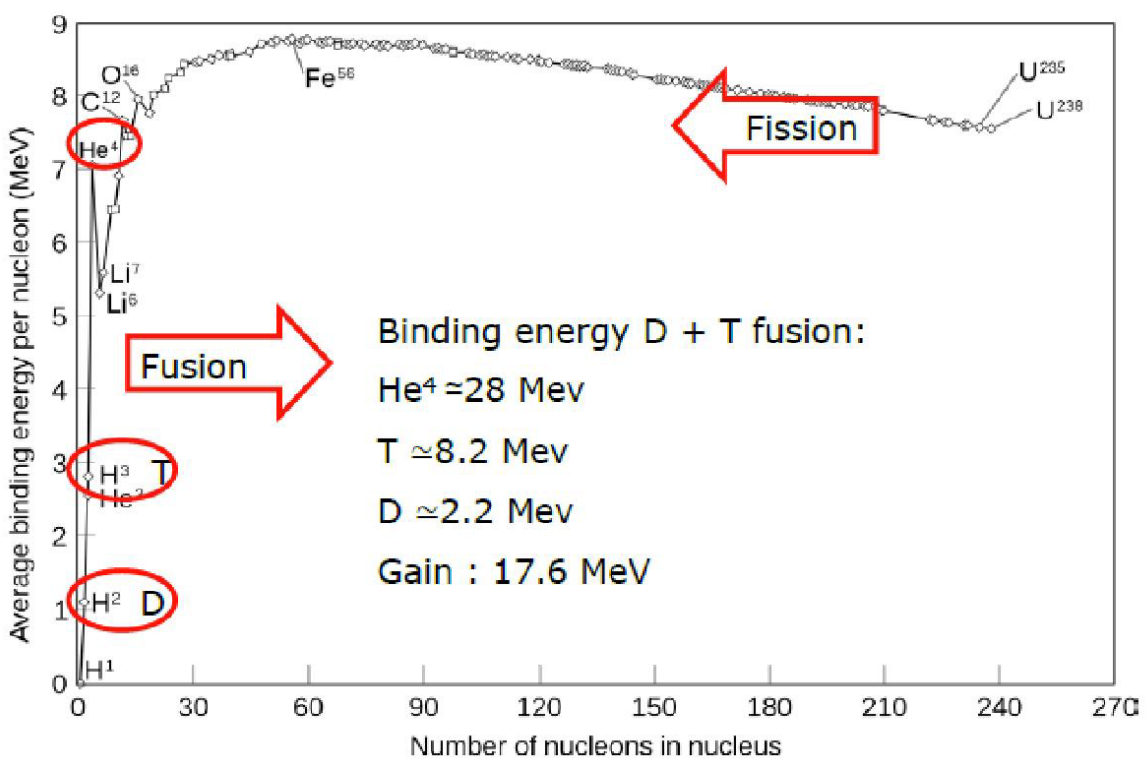
\includegraphics[width=\linewidth]{Chapters/chapter1/figs/binding energy.PNG}
	\caption{Average binding energy per nucleon \cite{YanNingNaulinVolkerWanBaonianXu2014}}
	\label{fig:binding_energy}
\end{figure}

Another factor to consider in comparing different fusion reactions is the likelihood of the reaction to happen. This is characterised by the fusion cross section, that depends on the kinetic energy of the incident particle. Considering an ensemble of particles this kinetic energy translate in temperature. The lower the temperature for which the cross section reaches its peak the easier to achieve fusion.
For this and other reasons the reaction that is the main focus of current research is the fusion of deuterium and tritium to helium: \cite{Miley1974}

\begin{equation}
{ }^2_1 D+ { }^3_1T \leftarrow { }^4_2He+{ }^1_0n
\label{eq:fuse}
\end{equation}

In this reaction are released 3.5MeV in kinetic energy of the alpha particle and 14.1MeV in the neutron. Tritium is not available in nature because it is radioactive with a short half life, so it must be produced. It is foreseen to produce it using the neutron released in reaction \ref{eq:fuse} in the reactions \ref{eq:fuse1} and \ref{eq:fuse2}

\begin{equation}
{}^{6}Li + n \leftarrow {}^{4}He +T +4.78MeV
\label{eq:fuse1}
\end{equation}

\begin{equation}
{}^{7}Li + n \leftarrow {}^{4}He +T +n +2.47MeV
\label{eq:fuse2}
\end{equation}

The initial fuels in this cycle then are deuterium and lithium, both widely available in nature.

\section{Plasma confinement}
%\hl{triple product, H mode, SOL, ELMs}

The temperatures that are relevant for fusion application are measured in keV, that correspond to millions of °C. At these temperatures matter is in the state of plasma, meaning that atoms are ionised and nuclei and electrons can move freely. These temperatures are of the same order of magnitude of the centre of the Sun. No material can withstand them so special techniques must be adopted to confine the reactant long enough for a significant fraction to fuse. The most important figure of merit of the achieved confinement is the fusion triple product, related to Lawson criteria, that returns the minimum product of plasma density, temperature and confinement time to achieve ignition (\autoref{eq:fuse3}). Ignition is the condition when the fusion power output is sufficient to maintain a constant temperature against all losses without external heating.

\begin{equation}
{n_e} {\tau }_{E} T_e  >=  5\cdot{10}^{21}{ m }^{ -3 }skeV
\label{eq:fuse3}
\end{equation}

The most viable way to maintain this environment is expected to be
through magnetic confinement, and specifically the tokamak (Magnetic Confinement Fusion, MCF).
In MCF the fuel is confined in plasma state thanks to its behaviour when exposed to electromagnetic fields. Every electrically charged particle is subject to Lorentz force:


\begin{equation}
F = q ( E+ vxB )
\label{eq:lorentz}
\end{equation}

In the presence of a magnetic field the particle gyrate with a circular motion in the direction perpendicular to field lines and is unperturbed in the parallel direction. In a tokamak the plasma is arranged in a doughnut shape, closely surrounded by two main set of coils: the toroidal field coils that generate the toroidal magnetic field and the central solenoid that with a time varying current induces a current through the plasma that generates the poloidal magnetic field. The toroidal geometry cause drifts in the plasma that would cause it to quickly reach the walls and cool down. To stabilise the plasma and shape it as requested other coils have to be added.\cite{Chen1974} The magnetic field generated in this way is composed of concentric flux surfaces that expand to the coils. The final configuration is outlined in \autoref{fig:mcf}. Shown in pink is a magnetic surface, that is the set of all the positions a particle can assume when streaming unimpeded following magnetic field line. JET is currently the largest tokamak and has achieved triple products higher than $10^{21} m^{-3}skeV$ in 1997 \cite{Gormezano1998} and recently the record for fusion energy produced of 59MJ. \cite{Gibney2022}

\begin{figure}[!ht]
	\centering
	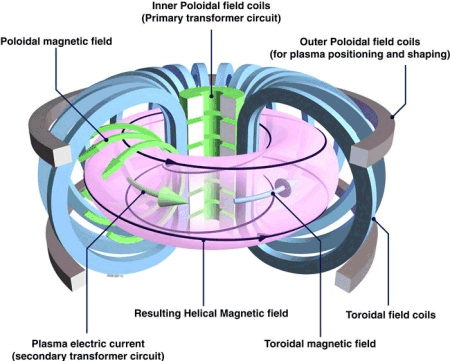
\includegraphics[width=0.7\linewidth]{Chapters/chapter1/figs/mcf.png}
	\caption{Schematic of the main components of a tokamak \cite{CulhamCentreforFusionEnergy2018}}
	\label{fig:mcf}
\end{figure}

The plasma can move freely along the field lines and slowly across it, so in time it drifts from the centre toward the wall via cross field transport caused by collisions and turbulence. One of the important evolutions of the tokamak design is to add a coil parallel to the plasma with a current in the opposite direction. This changes the magnetic configuration in such a way that the core of the plasma is not any more in direct contact with a solid limiter. The first magnetic surface that crosses solid surfaces from the core is referred as Last Closed Flux Surface (LCFS) or separatrix and where the poloidal field goes to zero is the x-point. The separatrix crosses the solid surfaces in well defined regions, called divertor targets. The plasma that escapes from the core (which state is usually referred to as "upstream") reaches the separatrix and then follows the magnetic field around the core and reaches the targets. In this way the core is shielded from the impurities generated by the plasma/surface interaction and can efficiently expel the fusion products. This motion along field lines is much faster than across and it is associated with a layer out of the LCFS called Scrape-Off Layer (SOL). The time a particle needs to cross the plasma from the centre and reach the wall defines the confinement time.

\section{H-mode}
A way to limit cross field transport in the core region and move towards ignition is to operate in the so called H mode. This regime is reached when the energy flux across the separatrix is increased over a threshold that depends on the discharge conditions.\cite{Ryter1998} The physics behind the specific value of the L-H threshold is still not fully understood, but its effect is to induce a transport barrier at the edge of the core plasma. This barrier strongly reduces the anomalous transport due to turbulence in a thin region around the core, allowing for a better energy and particle confinement there. One drawback of the H-mode is that it causes cycles of accumulation of energy in the core that is then released (up to 10\% of the core plasma thermal energy\cite{Zohm1996}) in sub ms bursts of hot plasma. These so called Edge Localised Modes (ELMs) cause a temporary increase of particle and thermal flux on the target of 2-3 orders of magnitude, that is expected to not to be tolerable in a large tokamak.\cite{Jachmich2011} The transport barrier is also very effective in confining impurities and fusion products in the plasma core.\cite{Putterich2011} This leads to a dilution of the fusion fuel and a possible radiative collapse of the plasma. ELMs are beneficial in this context as they provide a mechanism to transport impurities across the transport barrier.\cite{Leonard2014}

Various solutions to the ELMs problem have been put forward, in the form of different operational regimes where the instabilities that cause the ELMs are prevented or limited, but usually comport some degree of degradation of the confinement properties typical of the ordinary ELMy scenario, or a limitation of the operational space. Another solution is to 
cause intentionally more frequent and smaller events that can release part of the accumulated energy and particles in a more controlled and gradual manner.\cite{Leonard2014}

In order to sustain the H-mode a certain amount of power must cross the separatrix, otherwise the H-L back transition can occur. This constitutes a lower bound to the heat and particles that need to be dissipated from the separatrix to the target.

\section{The exhaust problem}
%\hl{thin SOL, melting/erosion}

The issue that arises with the divertor configuration is that the SOL is  very narrow, of the order of mm\cite{Faitsch2021,Silvagni2020}, and all the exhaust heat is delivered to a small area of the target. For ITER, a fusion device in construction in France that will be a step closer to a power production device, this heat is in the order of $GW/m^2$.\cite{Kuang2020} The widely used maximum power that can be removed from a surface with current technologies is $10-20MW/m^2$.\cite{Pitts2019,Lipschultz2018} If the heat to the target is not mitigated this will pose a serious limitation on its lifetime and the amount of impurities reaching the plasma, making impossible profitable operations. 
Sputtering is the phenomenon of emission of one or multiple atoms from a solid surface caused by interaction with an ion. This happens even for heat fluxes much lower than what is required for melting the surface.\cite{Wiesen2017a} There are various types of possible interactions but, as a whole, larger the energy of the ion larger number of atoms are sputtered from the surface. The local interaction of the plasma with a solid surface creates a sheath where the ions are accelerated towards the surface, exacerbating sputtering. The flow velocity at the sheath entrance amounts to $v_{se} \geq \sqrt{\frac{kT_e + \gamma kT_i}{m_i}}$ with $m_i$ the ion mass $k$ the Boltzmann constant, $\gamma=5/3$, $T_e$ and $T_i$ electron and ion temperature respectively, higher than the plasma sound speed $c_s \approx \sqrt{\frac{2kT}{m_i}}$. The sputtered atoms can end in the plasma, polluting it, or be redeposited to the target, changing its composition and properties. Sputtering can be so severe to be the main limiting factor of the lifetime of the plasma facing components.

\section{Divertor shaping}
%\hl{total/poloidal flux expansion}

The heat and particle flux can be reduced by tilting the target with respect to the separatrix, by locally reducing the magnetic field, thus spreading the heat on a larger surface and by moving the strike points to a larger radii to spread the heat on a larger surface.
Under investigation are different divertor designs (see some on \autoref{fig:divertor_geometry}) with the purpose, among others, to ease the thermal burden on the target

\begin{figure}[!ht]
	\centering
	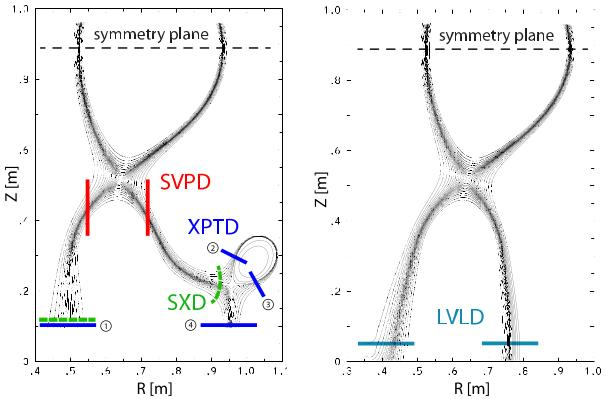
\includegraphics[width=0.8\linewidth]{Chapters/chapter1/figs/divertor geometry.jpg}
	\caption{Example of different divertor configurations. Left:Standard Vertical Plate Divertor (SVPD), Super-X Divertor (SXD) and X-point Divertor (XPTD). Right: Long Vertical Leg Divertor (LVLD) \cite{Umansky2017}}
	\label{fig:divertor_geometry}
\end{figure}

The above mentioned effects combined lead to a reduction of the heat flux density around 20 times for a tokamak of SVPD divertor type like will be on ITER, still short of another 10 times reduction needed to respect the $10-20MW/m^2$ limit. The divertor configuration introduces an asymmetry in the toroidal geometry due to the two targets located at different radii. In terms of energy and particle redistribution in the SOL the inner target will receive a higher ion flux and lower energy flux compared to the outer one. As it will become clear later, on the inner target this causes stronger recycling and eases the thermal load, while the outer target is normally subjected to more severe conditions. [\cite{Potzel2014} and references there therein]

\section{Radiative dissipation scenario}\label{Radiative dissipation scenario}
%\hl{energy removal --> radiative scenario, impurities}

Another way to decrease the heat flux to the target is to induce radiation in the SOL.
Radiation occurs naturally in plasmas and it depends greatly on temperature and density of each specie. When an atom is not yet fully ionised the electronic levels can be excited by collision and de-excite emitting a photon. The ionised atoms can recombine with free electrons and release a photon too. The energies at which these effects are more likely correspond to the peaks in the curves in \autoref{fig:loss_curve}. If the temperature is so high that atoms are fully ionised the only radiative mechanism is Bremsstrahlung radiation, that is much less efficient. This corresponds to the monotonic increasing right part of the curves in \autoref{fig:loss_curve}.

\begin{figure}[!ht]
	\centering
	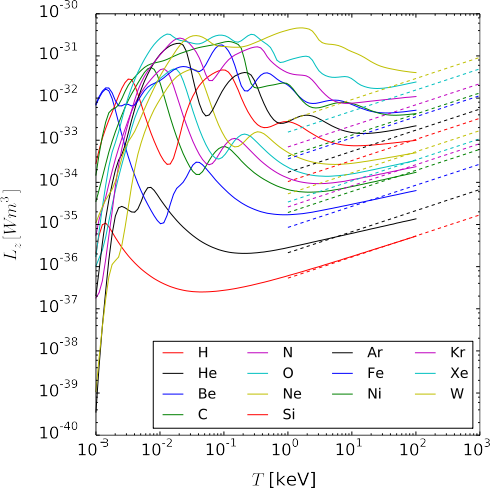
\includegraphics[width=0.7\linewidth]{Chapters/chapter1/figs/loss curve.png}
	\caption{Loss function data from the ADAS data base (solid lines) for the different elements \cite{Lux2015}}
	\label{fig:loss_curve}
\end{figure}

At the temperatures of interest in the SOL (100s of eV\cite{Pacher2011}) hydrogen is fully ionised and radiates weakly. With the addition of impurities sputtered from the wall or specifically seeded in the discharge the energy can be transferred from the plasma to the impurities and then radiated. This mechanism can be exploited to dissipate a significant amount of power from the core and edge of the plasma, but also the SOL. This regime is referred to as the radiative scenario.


\section{Detachment}\label{Detachment}
%\hl{particle removal -> recycling, detachment}

At low upstream densities the plasma that enters the SOL can flow relatively unimpeded towards the target. The temperature in the SOL is about constant and the particle flux is limited only by the sheath condition (e.g. "sheath-limited"). By increasing the core and SOL density plasma heat flux conductivity decreases (e.g. "conduction limited"), leading to negative gradients of the temperature and positive of the density, with an almost uniform pressure. The heat flux to the target is the sum of the component parallel to field lines $q_{par}$, the orthogonal one $q_{ort}$ and a component given by the energy released with recombination $q_{rec}$, given by  \autoref{eq:detachment}.

\begin{equation}
\begin{aligned}
{ q } _{ par } =& { n } _{ e,t } { c } _{ s } {  \gamma  } _{ sh }{ k } _{ B }{ T } _{ e,t } \; \alpha \; { p } _{ e,t }{{ T } _{ e,t }}^{0.5 } \\
{ q } _{ ort } =& { q } _{ par } \left( \frac {{ B } _{ p }} {{  B  }_{ \phi  }}   \right) _{ t} \; \alpha \; { p } _{ e,t }{{ T } _{ e,t }}^{0.5 } \\
{ q } _{ rec } =& { n } _{ e,t } { c } _{ s } {  E  } _{ pot } \; \alpha \; { p } _{ e,t }{{ T } _{ e,t }}^{-0.5 }
\end{aligned}
\label{eq:detachment}
\end{equation}

where $\gamma_{sh}$ is the heat sheath transmission factor, $n_{e,t}$ and $T_{e,t}$ are the electron density and temperature in front of the target, $c_s$ is the sound speed, $B_p$ and $B_{\Phi}$ are the poloidal and toroidal magnetic field and $E_{pot} \approx 15.8 eV$ is the potential energy released per ion when recombining to neutral deuterium molecules on the target plate. \cite{Reimold2015} The temperature cannot be indefinitely reduced because of operational limits like the Greenwld limit.\cite{Greenwald1988} Moreover, a reduction of the temperature does not alone guarantees a decrease of the heat flux.  One possible solution to achieve it is to cause gradients of temperature and pressure along the field lines in the SOL. This should be done in such a way to minimize the impact on the core plasma.

A way to achieve this is to induce plasma detachment. This phenomenon has been observed in a series of tokamaks [\cite{Reimold2015} and references therein] and can be induced by impurity seeding or fuelling. In Alcator C-Mod \cite{Lipschultz2007} and AUG \cite{Kallenbach2015a} it was shown to significantly reduce target heat flux in conditions scalable to burning plasmas like ITER.

In an attached regime the plasma streams through the SOL and reaches the target. At the target the charged particles recombine and become neutrals. They are generated in an excited state therefore a strong radiation at the strike points. The neutrals are not bound by magnetic fields, and can move freely until they collide with other neutrals or particles from the plasma. A neutral can then re-ionise and stream along field lines, returning to the target or entering the plasma again. This process is called recycling and the region of the leg where it occurs the ionisation or recycling region.

If the density in the SOL is high enough the neutrals generated at the surface by the plasma will interact mainly in the SOL and the plasma will loose part of its energy and momentum on its way to the target via radiation and transport.\cite{Leonard2018} To further increase the energy loss low Z impurities like Nitrogen can be seeded in the SOL: they will ionise only partially, radiating efficiently at higher temperature than hydrogen or helium. The lower the temperature the higher the energetic ionisation cost. This because lower temperature means smaller progressive excitation by collisions of the bound electron up to ionisation with radiative losses in the process, instead of a single higher energetic collision directly to ionisation. This causes even more radiative cooling. In most cases, and especially if the divertor is baffled like in the Mega Ampere Spherical Tokamak Upgrade (MAST-U) tokamak, allowing for a higher neutral density inside, the volumetric ionisation source from neutrals constitute the main source of ions for the target flux.\cite{Krasheninnikov2016,Krasheninnikov2017a,Lipschultz1999} This is referred to as high recycling, where the recycling region constitutes a self-contained system that is supplied from upstream mainly of energy. This is believed to be one of the most important difference between tokamak divertors and linear machines, where the main source of ions is usually the plasma source upstream. Simulations for the linear machine Pilot-PSI, characterised by a very high density, show that ionisation could account for up to a third of the plasma source, but this in a region very close to the source itself.\cite{Jesko2018,Hayashi2016}

From detachment experiments it is observed that the particle flux to the target increases with increasing core density. Increasing further the density or impurity seeding the particle flux reaches a maximum and then decreases. This is called rollover and corresponds with the onset of detachment. Other metrics for the detachment offset have been used, as the decrease of the target temperature below a certain threshold\cite{Stangeby2000,Goldston2017}, but the Langmuir probe constitute a direct and simple measurement, hence their widespread use. Pushing the process forward the particle flux decrease and saturates. In the case the plasma could loose all its kinetic energy, or temperature, it still maintains the energy associated with its creation, the ionisation and dissociation energy, $15.8eV$. In a DEMO scale device this residual energy flux would be still high enough to exceed the $10-20 MWm^{-2}$ limit on the target. \cite{Krasheninnikov2017a} To reduce it even further the temperature must drop below $1eV$ to trigger volumetric recombination. This is accompanied by a strong radiation increase from where volumetric recombination occurs. The particle flux drop can continue up to the point that the measured plasma temperature at the target reaches a minimum and the radiating region (radiation front) recedes upstream along the field lines.\cite{Krasheninnikov1999} at different stages in this process different fronts will in turn detach from the target line the ionisation and thermal front.\cite{Hutchinson1994,Loarte1998,Lipschultz2016} The fronts movement comes from the balance between the power and particles entering the SOL with dissipation by radiation and interaction with recycling neutrals.


% \section{Atomic and molecular processes}
% \hl{
%             1. attached $->$ hot $->$ atomic physics
%             2. detached $->$ cold $->$ atomic and molecular physics}


\section{The x-point radiator}\label{The x-point radiator}
%\hl{extreme end of detachment before MARFE, increased radiated power}

When a discharge, both L-mode and H-mode, is close to the detachment threshold in a tokamak with a conventional divertor configuration and the impurity or core density is increased, 4 stages of detachment are defined as per the description in \cite{Reimold2015,Potzel2014} (here with detachment is intended the particle flux roll over and deviation from the attached case scaling, see \autoref{Analytic models}).

\begin{enumerate}
    \item Onset of detachment: the inner target detaches inter-EMLs (even due to recycling and without impurity seeding), the outer target is attached
    \item Fluctuating state: radiative fluctuations in the kHz appear at the X-point, inner target detaches inter-EMLs
    \item Partial detachment at outer target: inner target always detached, outer target detached inter-ELMs, strong radiation at the X-point, fluctuations frequency decrease to ELMs scale, ELMs amplitude decrease.
    \item Complete detachment: inner and outer target always detached, sporadic ELMs, radiator moves from X-point further into the confined plasma
\end{enumerate}

For this type of discharge the radiator close to the X-point appears when detachment starts at the inner target, while it is only enhanced by the detachment on the outer target. Because the parameter of interest is the reduction of thermal flux on the outer target a feature that will always be present in reactor relevant conditions is a strong radiator located close to the X-point.

If the density is further increased, the radiator can move either vertically upwards entering the core\cite{Bernert2021} or move along the inner separatrix up to the midplane and enter the core from there.\cite{Lipschultz1984} In both cases a degradation of the confinement properties is observed.

\section{Effect of X-point radiator}\label{Effect of X-point radiator}
%\hl{poloidal asymmetry, pedestal flattening, loss confinement}


The X-point radiator (XPR)\cite{Bernert2021} or X-point MARFE\cite{Kallenbach2015a} is a region of steep temperature gradient, where the temperature goes from that of the hot upstream plasma from the core to the cold region where ion / neutral interactions dominate. The presence of such a thing at or inside the separatrix can lead to confinement degradation. In this context what is referred as confinement H98 is the ratio of the actual energy confinement time $\tau_{th}$ over a reference. The reference is a confinement time from a scaling law obtained fitting the confinement time of many tokamak experiments in a certain operating mode. For ELMy H-mode the scaling law mostly used is the ITER Physics Basis (IPB) 98(y,2).\cite{Doyle2007} For L-mode the ITERL-97P scaling can be used. \cite{Kaye1997} The scalings are given by \autoref{eq:h98y2} and \ref{eq:l97}. For spherical tokamaks an H-mode \cite{Kaye2006} and MAST L-mode \cite{Kaye2021} scaling are given in \autoref{eq:HST}, \ref{eq:LST} respectively.


\begin{equation}
{ H }_{ 98 }={\tau }_{ th }/{\tau }_{ th,98y2 } \; , \; {\tau }_{ th,98y2 }=0.0562 {{ I }_{ P }}^{ 0.93} {{ B }_{ t }}^{ 0.15} {{ n }_{ 19 }}^{ 0.41} {{ P }_{ L }}^{ -0.69} {{ R }_{  }}^{ 1.97} {{ \varepsilon  }_{  }}^{ 0.58} {{ \kappa  }_{ a }}^{ 0.78} {{ M }_{  }}^{ 0.19}
\label{eq:h98y2}
\end{equation}

\begin{equation}
{ L }_{ 97 }={\tau }_{ th }/{\tau }_{ th,97P } \; , \; {\tau }_{ th,97P }=0.037 {{ I }_{ P }}^{ 0.74} {{ B }_{ t }}^{ 0.2} {{ n }_{ 19 }}^{ 0.24} {{ P }_{ L }}^{ -0.75} {{ R }_{  }}^{ 1.69} {{ \varepsilon  }_{  }}^{ 0.31} {{ \kappa  }_{ a }}^{ 0.67} {{ M }_{  }}^{ 0.26}
\label{eq:l97}
\end{equation}


\begin{equation}
{ H }_{ ST }={\tau }_{ th }/{\tau }_{ th,HST } \; , \; {\tau }_{ th,HST }=0.066 {{ I }_{ P }}^{ 0.53} {{ B }_{ t }}^{ 1.05} {{ n }_{ 19 }}^{ 0.65} {{ P }_{ heat }}^{ -0.58} {{ R }_{  }}^{ 2.66} {{ \kappa  }_{ a }}^{ 0.78}
\label{eq:HST}
\end{equation}

\begin{equation}
{ L }_{ ST }={\tau }_{ th }/{\tau }_{ th,LST } \; , \; {\tau }_{ th,LST }=0.153 {{ I }_{ P }}^{ 1.01} {{ B }_{ t }}^{ 0.7} {{ n }_{ 19 }}^{ -0.07} {{ P }_{ L }}^{ -0.37}
\label{eq:LST}
\end{equation}

With $I_P$ plasma current in $MA$, $B_t$ toroidal magnetic field in $T$, $n^{19}$ averaged electron density in units of $10^{19} \#/m^3$, $P_L=P-dW/dt$ power loss in $MW$ with $P$ heating power and $W$ stored energy, $R$ major radius, $a$ minor radious, $\varepsilon=a/R$ inverse aspect ratio, $\kappa _a$ elongation, $M$ ion mass number in $amu$.
It is possible to calculate the energy confinement time from magnetic coils measurements and the energy transferred to the plasma as heating ($P_{heat}$). $\tau_{th}$ is defined by 

\begin{equation}
\begin{split}
\frac {dW} {dt}={P}_{heat} - \frac {W} {\tau }_{ th } \; , \; W=\frac { 3} {2} \langle p \rangle V \; , \; \langle p \rangle = \frac {{ \mu }_{ 0 } {{ I }_{ p }}^{ 2 } { \beta }_{ p }} { 8 {\pi}^{2} {a}^{2}  } \\ {\beta }_{ p } = \langle \frac { n {k}_{B} T} { {{B}_{p}}^{2} /(2 {\mu}_{0}) } \rangle \; , \; {P }_{ heat }={ P }_{ ohmic }+{ P }_{ NBI }+{ P }_{ RF }
\label{eq:tau}
\end{split}
\end{equation}


With $V$ plasma volume, $\langle p \rangle$ volume-averaged plasma kinetic pressure, ${{ \beta }_{ p }}$ poloidal beta, $B_p$ poloidal magnetic field, $a$ minor radius, $P_{ohmic}$, $P_{NBI}$, $P_{RF}$, power transferred to the plasma by ohmic heating, neutral beam injector and radio frequency respectively. \cite{SalarElahi2010,Fallis2013} The confinement loss is usually done comparing before and after the appearance of the X-point radiator, or with a series of discharges in similar conditions but without and without X-point radiator.
The confinement degradation can be due to the direct cooling caused by the cold region (e.g. poloidal temperature gradients to drive power to that location \cite{Lipschultz1998} ) or to easier penetration of impurities in the core [\cite{Lipschultz2016} and references therein]. The degradation significantly affects the outer part of the core region with significant reduction of temperature, pressure and an increase of density. \cite{Kallenbach2015a}  It was found on some experiments that the inner core (ratio of poloidal magnetic flux over poloidal magnetic flux at the separatrix $ \rho _{pol}<0,8-0,5 $) is only marginally effected. [\cite{Reinke2013} and reference therein] It is therefore suggested that the gradients lost on the pedestal region could be recovered in a portion of plasma $0,8< \rho _{pol}<0,95$. \cite{Reimold2015}

The X-point radiator will also have the effect of radiating a substantial fraction ($75-90\%$ of the heating power achieved \cite{Bernert2017}) of the total $ \alpha $ particles / heating power out of the separatrix and could cause the H-L transition. This is anyway not a major risk for ITER and larger machines, because the power crossing the separatrix is expected to be significantly larger that the threshold requirement. It has been in fact considered to seed a higher-Z impurity in the plasma to enhance core radiation (radiative mantle) and lower the power needed to be exhausted through the separatrix to about the minimum for the L-H transition. Then a lower-Z impurity will be fed to radiate in the divertor. [\cite{Kallenbach2015a,Reinke2013} and reference therein]


There are two active areas of research to limit confinement losses with XPR.

One is in trying to achieve detachment but not allow the radiator moving all the way to the X-point and cause confinement degradation. The main difficulty in achieving this is that, for standard divertor geometries the operational window of any given control parameter to move the radiator from target to X-point is very narrow. Considerable effort has been put forward to find a predictive model. An early attempt is the two point model, a 1D model where the conditions outside the separatrix and at the target are correlated adopting some approximations on the heat and particle transport.\cite{HOBBS1966,Hobbs1967,Mahdavi1981,Keilhacker1982,Harbour1984,Lackner1984,Stangeby2001} The thermal front model proposed by Lipschultz \cite{Lipschultz2016} is an improved 1D model that, balancing input / output power on the thermal front (edge of the radiator toward the core), tries to identify the operational window of a control parameter and its stability for given plasma / magnetic configuration. This model finds that for all the control variables analysed the operational window widens for increasing ratio of X-point over target magnetic field $B_x/B_t$ and ratio of the connection length between X-point and target over upstream and target $z_X/L$. It is also found that increasing connection length should lower the detachment upstream density threshold. Stability analysis indicates that for decreasing $z_X/L$ there is an increasing minimum Bx/Bt for a stable solution.\cite{Lipschultz2016}

This puts additional emphasis on research on different divertor designs. TCV in Switzerland and MAST-U in UK are the best suited for this type of investigations due to the flexibility of their divertor geometry. Recent data from TCV seems to prove that the sensitivity on control parameters decreases with flux expansion (larger operational window) but didn’t verify the threshold dependence on connection length. \cite{Theiler2017}

A second strategy is to live with the radiator located at the X-point (it’s further apart from the target, ELMs have to burn through more divertor volume before reaching the target) and try to understand and minimize the loss of confinement in the core. The reality of present conventional tokamaks is that the X-point radiator always appears if full detachment from the target is pursued, with different flavours depending on the seeded impurity as it can be seen in \autoref{fig:xprs}.

\begin{figure}[!ht]
	\centering
	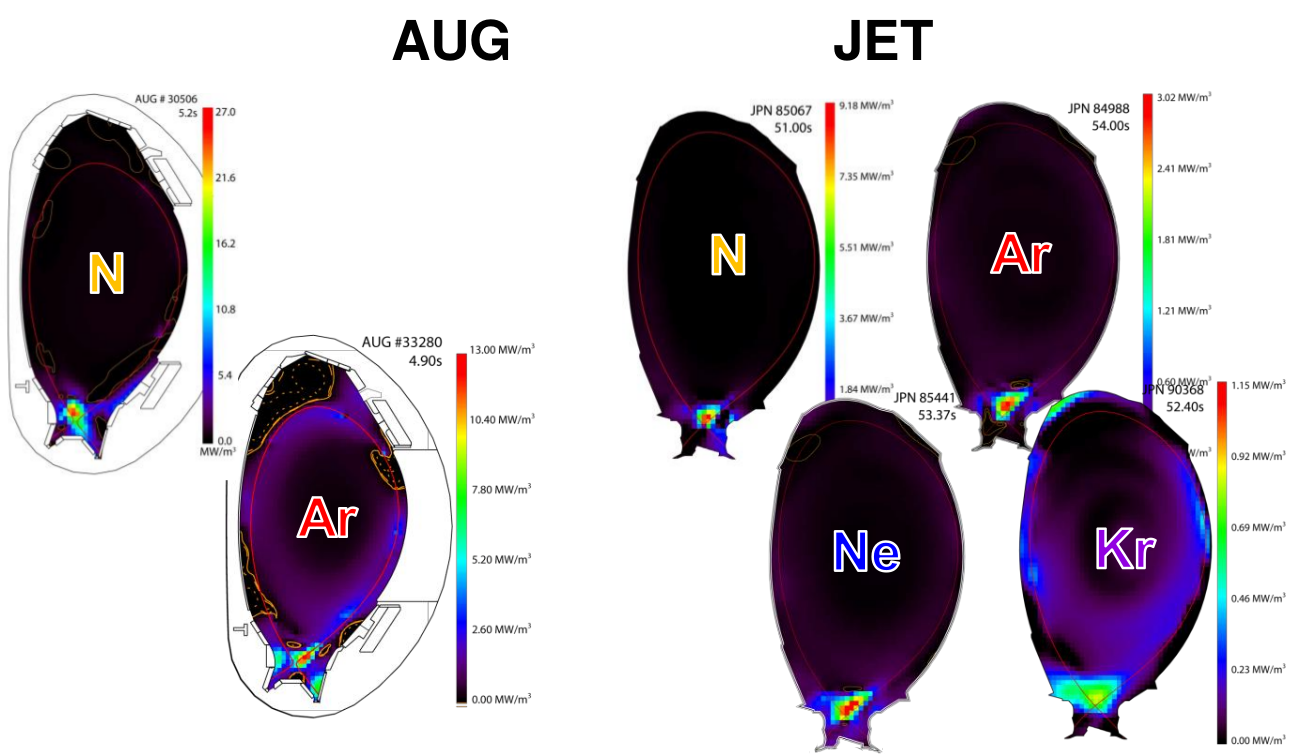
\includegraphics[width=\linewidth]{Chapters/chapter1/figs/xprs.png}
	\caption{Different radiation profiles with clear presence of X-point radiator for different impurities
	\cite{Wiesen2017}}
	\label{fig:xprs}
\end{figure}

The X-point radiator cannot be idealised as easily as the thermal front of detachment, because it is much more related to core and edge dynamics. Modeling its behaviour requires the use of codes that accounts for all atomic interactions, drifts, etc. like SOLPS-ITER, EDGE2D-EIRENE, SOLEDGE2D-EIRENE [\cite{Wiesen2017a} and references therein]. The presence of the radiator significantly affects temperature, pressure and density distribution, especially in the pedestal, therefore it is likely to have an effect on the current distribution and MHD activity.
In the last years a large effort has been put forward in the characterisation of the behaviour of the X-point radiator and its macroscopic effects on the core / edge. This has been done mostly in conventional geometry tokamaks, both with metal and carbon wall.


\section{ELMs and XPR}
Another important feature of the XPR is the reduction in amplitude of ELMs. This can be attributed to the fact that the energy associated with the ELM first heats up the XPR and then moves toward the target. If the neutral density between X-point and target, and in the radiator itself, is high enough it could be possible to avoid ELMs to “burn through” the detachment front and to reach the target altogether. \cite{Krasheninnikov2016} This can be further improved by some divertor configurations like the super-x divertor with a long outer leg, in that the ELM has more time to interact the cold gas and dissipate some of its energy. The burn through is a complex phenomena because of the short time scale (hundreds of $\mu s$), complex geometry and complex interactions between the core plasma being expelled by the ELM and the neutrals. Simplified simulations have been carried out to study the dynamic of the burn through in MAST-U showing a significant reduction of the peak target heat flux compared to empirical scalings.\cite{Smith2020,Smith2020a}


\section{Analytic models}\label{Analytic models}

In order to qualify and characterise the evolution of detachment it is useful to build approximate analytical models for the properties of interest, like particle and power fluxes, depending of the upstream plasma conditions. The most widely model is the two point model (2PM) and its variations.\cite{HOBBS1966,Hobbs1967,Mahdavi1981,Keilhacker1982,Harbour1984,Lackner1984,Stangeby2001} In it the complex 3D geometry of the SOL is translated to a simpler 1D system as shown in \autoref{fig:2PM}.

\begin{figure}[!ht]
	\centering
	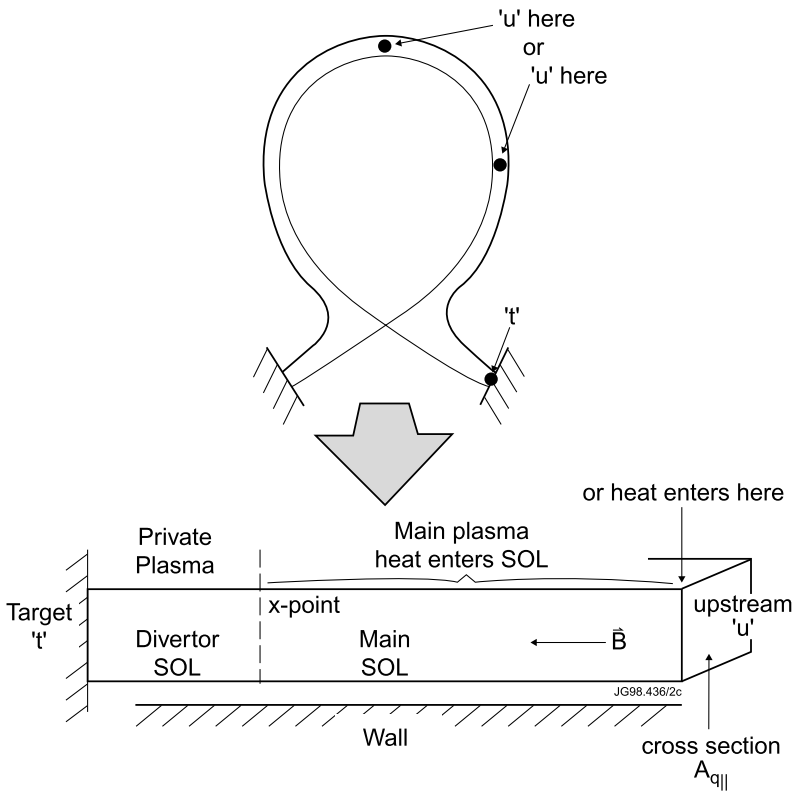
\includegraphics[trim={0 0 0 0},clip,width=0.65\linewidth]{Chapters/chapter1/figs/2PM.png}
	\caption{Schematic of how the poloidal SOL geometry can be straightened into a 1D one. The model is weakly sensitive to the location of the upstream location, assuming gradients are weak far from the divertor.\cite{Verhaegh2018} Adapted from \cite{Harrison2011} and the JET image database.}
	\label{fig:2PM}
\end{figure}

Then a series of assumptions are done:
\begin{itemize}
    \item There are no power losses along the SOL, excluding all radiated power losses.
    \item Ionisation does not affect the energy and flow profile.
    \item Heat is transported only via parallel heat conduction.
    \item Plasma pressure is considered constant in the entire SOL.
    \item Quasi neutrality and same temperature for electrons and ions ($n_e = n_i = n$, $T_e = T_i = T$).
    \item All the power to the SOL is transferred at the upstream location.
\end{itemize}

At the target surface the presence of the sheath accelerate the ions to the sound speed, so the local pressure given by the static and dynamic component $p_t$ is

\begin{equation}
p_{t} = p_{static} + p_{dynamic} = 2n_{t} k T_{t} + n_{t} m_i {{c_s}_t}^2
\label{eq:2pm1}
\end{equation}

Upstream the velocity component to the pressure is negligible so $p_u \approx 2 n_u k T_u$ so considering the pressure is uniform this returns the first equation of the 2PM

\begin{equation}
2 n_u k T_u = 2n_{t} k T_{t} + 2n_{t} k T_{t} \rightarrow n_u T_u = 2n_{t}T_{t}
\label{eq:2pm2}
\end{equation}

Since no volumetric power loss is considered the heat transferred to the SOL streams freely to the target, and it is determined by the sheath as

\begin{equation}
q_{\parallel} =  \gamma n_t k T_t {c_s}_t = \gamma n_t \sqrt{\frac{2(kT_t)^3}{m_i}}
\label{eq:2pm3}
\end{equation}
returning the second equation of the 2PM.

This heat is carried to the target via conduction. In order to calculate it, one should consider that the parallel heat conductivity for charged particles self-collisions can be written as ${v_{th}}_s mfp_s \approx {{v_{th}}_s}^2/{\nu_s}$ with ${v_{th}}_s$ the unidirectional thermal velocity of the species $s$, $mfp_s$ the self-collision mean free path and $\nu_s$ the self-collision frequency. ${v_{th}}_s$ is given by $\sqrt{8kT_s/{m_s}}$ while $\nu_s$ is proportional to $n_s/\sqrt{m_s T_s^3}$. The heat conductivity is then proportional to $ {T_s}^{5/2} / {m_s}^{1/2}$. This indicates that, given the mass difference, electrons dominate the conduction heat transfer, and that there is a strong dependency on the temperature. The heat flux can then finally be written as per \autoref{eq:2pm4a} where the electron parallel heat conductivity coefficient $\kappa$ is of the order of 2000.\cite{Stangeby2001}

\begin{equation}
q_{\parallel} = -\kappa T^{5/2} \frac{dT}{ds_{\parallel}}
\label{eq:2pm4a}
\end{equation}

This equation can be integrated from upstream to target (amounting to the connection length $L$), and considering that $q_{\parallel}$ is constant one can obtain the last equation of the 2PM model

\begin{equation}
{T_u}^{7/2} = {T_t}^{7/2} + \frac{7 q_{\parallel} L}{2 \kappa}
\label{eq:2pm4}
\end{equation}

Assuming fixed $q_{\parallel}, L, \gamma, m_i$ \autoref{eq:2pm2}, \ref{eq:2pm3} and \ref{eq:2pm4} contain 4 unknowns ($n_t, n_u, T_t, T_u$) and can be used to numerically solve for 3 when one is known or measured. If one assumes $T_u >> T_t$ as it is the case in the conduction limited regime, \autoref{eq:2pm4} can be further simplified neglecting $T_t$ and the 2PM reduces to

\begin{equation}
\begin{aligned}
T_t =& \frac{{q_{\parallel}}^2}{{n_u}^2 {T_u}^2} \; \frac{2m_i}{\gamma^2} \\
n_t =& \frac{{n_u}^3 {T_u}^3}{{q_{\parallel}}^2} \; \frac{\gamma^2}{4m_i} \\
T_u =& \left( \frac{7 q_{\parallel} L}{2 \kappa} \right)^{2/7}
\end{aligned}
\label{eq:2pm5}
\end{equation}

The target particle flux can finally be calculated as the heat flux over the energy released by each particle (neglecting the energy from surface recombination) from \autoref{eq:2pm3} as per \autoref{eq:2pm6} (the arrow refers to the further simplification as per \autoref{eq:2pm5}).

\begin{equation}
\Gamma_t = \frac{q_{\parallel}}{\gamma T_t} =  n_t \sqrt{\frac{2kT_t}{m_i}} \rightarrow \frac{{n_u}^2 {T_u}^2}{q_{\parallel}} \; \frac{\gamma^2}{2m_i}
\label{eq:2pm6}
\end{equation}
This correlation is the one that have been used in the literature to find detachment. The particle flux from Langmuir probes and the expectation from this scaling roughly match for an attached target. Increasing the upstream density further the particle flux plateaus then starts to decrease, deviating from the expected trend. This can be quantified in the Degree of Detachment (DoD) given by the ratio of the two quantities.\cite{Stangeby2001,Loarte1998}

This simple model can then be improved by including more of the true physics of the divertor and SOL like: volumetric power and momentum losses due to interactions with neutrals, volumetric radiated power losses, variation in $q_{\parallel}$ and pressure along field lines, sharp transition regions from x-point to target (e.g. ionisation / density / radiation front), magnetic configuration, etc.\cite{Stangeby2001,Cowley2022,Reinke2017,Lipschultz2016} This increase of sophistication allows, depending on the model, to also study the conditions along the leg, to investigate the relevance of different phenomena and the stability of the fronts movement. The fronts stability is particularly important because, as detached scenarios are more and more expected to provide the volumetric dissipation required for the target survival, it is paramount to be able to control their location. It has also been demonstrated that the threshold for rollover is proportional to a certain value of the ratio $ \frac {q_{rec}} {p_{up}}$ ($q_{rec}$ is the specific energy flux into the hydrogen recycling region). \cite{Krasheninnikov1999,Krasheninnikov2016,Stangeby2018}

Of relevance for the present work is that the depth of detachment increases with upstream density. This will be used to characterise density ramps in MAST-U during the first experimental campaign (MU01).

\section{Goals and objectives of the thesis}

The main objective of this work is to understanding of the radiation distribution on MAST-U and its relation to detachment. This is achieved with the design, implementation, calibration, validation and use of  the new infra-red video bolometer diagnostic in MAST-U. As it will be shown in detail in \autoref{chapter2}, the diagnostic is based of previous work on NSTX-U\cite{VanEden2016} and Alcator C-Mod\cite{Reinke2018a} and its goal is to measure the radiation distribution in the lower section of MAST-U with particular emphasis on the x-point region.

Significant work was necessary to design the system and to balance the strength of the signal with the desire to maximize spatial resolution (see \autoref{MAST-U IRVB design}). For this, new and accurate ray tracing methods were used in order to accurately determine the intensity of the radiation from the plasma on the diagnostic.

Once the diagnostic was built it was necessary to calibrate it, in order to convert the data to a from related to the power radiated by the plasma (see \autoref{System calibration}). This was done characterising all parts of the diagnostic and by finally verifying its accuracy compared to a known source. Once installed on MAST-U the orientation and the field of view was verified using features of the plasma, obtaining good agreement with the original design.

Finally the data from MAST-U is collected and analysed (see \autoref{MU01 Line integrated results}). The changes of line integrated brightness in different region of the plasma correlated well with the progress of detachment. The measurements match observations from other diagnostics that observe the total radiated power (resistive bolometry system), albeit being negatively effected by imperfections in the sensing element and a signal from the NBIs unrelated to the radiated power effecting part of the field of view.

In parallel to the hardware development an effort was undertaken to develop inversion routines capable to tomographically invert the line integrated brightness to emissivity (see \autoref{Inversion techniques}). Different methods were tested and a probabilistic approach was adopted to take into account the uncertainties arising from the different parts of the system.

The results show, for the first time in a spherical tokamak, the changes of radiation distribution in relation with detachment with high spatial resolution (see \autoref{MU01 tomographycally inverted results}). The movement of the radiation in the inner and outer leg can be compared with literature\cite{Reimold2015,Potzel2014,Lipschultz1984,Bernert2021} and it is found that the progression is similar to expectations in L-mode, while it wasn't in the H-mode discharges examined. This could be due to the H-mode scenario being not fully developed during the first experimental campaign of MAST-U. The progress of detachment in L-mode is compared to measurements from other diagnostics. The particle flux on the outer target is observed to consistently roll-over after the radiation is detached on the inner target and at the same time as the outer target radiatively detaches.
The radiated power in the core region scales well with measurements from the resistive bolometry system while the total power radiated in the super-x chamber is used in conjunction with measurements of the hydrogen and carbon line emission to confirm recent results on the processes involved with detachment\cite{Verhaegh2022} and the importance of molecular assisted reactions as intermediate step between electron impact ionisation and electron-ion recombination.

A secondary goal of this work, developed thanks to a collaboration with the DIFFER institute, The Netherlands,is understanding the behaviour of ELM-like pulses during detachment and the role of atomic and molecular processes. This was achieved conducting a series of experiments on the linear plasma machine Magnum-PSI, and upgrading the existing optical emission spectrometer to operate intra-shot measurements, as detailed in \autoref{chapter3}.

Conditions similar to the end of a target in a tokamak were reproduces, changing the neutral pressure to cause the target to transition from attached to detached. Superimposed to this steady state regime ELM-like pulses are recreated with a dedicated power supply system. These are a sudden increase of the plasma temperature and density such that the heat flux increase transiently by 1 order of magnitude. Time and spatially resolved measurements are taken with different diagnostics to understand the burn through process. This is difficult to do in a tokamak because of the poor diagnostic access and reproducibility, which are instead the strength of a linear plasma machine.

Direct measurement from a fast camera observing tangentially the burn through process and an infrared camera observing the target are used to determine that, when the neutral pressure is sufficiently high, the ELM-like pulse is prevented from effecting the target and the plasma is dissipated in the volume instead.

The measurements from the optical emission spectrometer were used in conjunction with other diagnostics to build a Bayesian algorithm capable of inferring the most likely properties of the plasma poloidally and temporally resolved. This is used to show, similarly to what done in the study on MAST-U, the importance of molecular assisted reactions. molecular processes are important in the exchange of potential energy, while less so in radiating the energy from the ELM-like pulse. It is also found that for some conditions the volumetric ionisation source is more important than the plasma input from the source, making this conditions closer than other linear machines to what observed in tokamaks.


% \subsection{XPR/radiation front location and confinement (maybe the dataset is not there)}
% find limit where confinement is not compromised, correlation between confinement and XPR/radiation location
% \subsection{poloidal (toroidal?) divertor after XPR}
% radiation spreading over all the separatrix, trasforming it into a limiter for the plasma.
% \hl{I never observed this, is it worth mentioning?}
% \subsection{XPR/detachment and power balance}
% radiator location vs radiated power
% \subsection{radiation front location and analytic models}
% DOD vs radiator location, radiation front range/stability vs prediction
% % \subsection{detachment and configuration (CD/SXD)}
% % radiated power vs configuration (against predictions)
% \subsection{radiation location and other metric of detachment}
% radiator location vs MWI/LP compared to expectations, ionisation/MAR/recombination region (Kevin work)
% % \subsection{XPR and ELMs}
% % ELMs burn through/impact on LP and IR vs detachment/radiation front location
% % \subsection{Cyd Cowley paper}
% % hysteresis in inner leg detachment
% \subsection{ELMs baffled in linear machine}
% Magnum work, it is possible to prevent ELMs to reach the target with target pressure
% \subsection{atomic vs molecular effects during ELMs burn through in deep detachment in linear machine}








\chapter{MASTU activities}\label{chapter2}

\section{Motivation}\label{Motivation IRVB}
% \hl{detachment, power balance, radiation front location, XPR literature on MAST-U}

\fbox{\begin{minipage}{\linewidth}%{15em}
Parts of this chapter have been adopted from:

F. Federici, M. L. Reinke, B. Lipschultz, A. J. Thornton, J. R. Harrison, J. J. Lovell, and M. Bernert. Design and implementation of a prototype infrared video bolometer (IRVB) in MAST Upgrade. \emph{Review of Scientific Instruments}, 2023.
\end{minipage}}
\\

As explained in \autoref{chapter1} the location of the radiating regions can have a significant impact on the core plasma.\cite{Reimold2015}. It is important, therefore, to well characterise the power balance and radiated power profile in current machines to understand the stability and performance of strongly radiating plasmas and support predictions for future devices. 
Key diagnostics are bolometers that usually operate by exposing a thin foil to plasma radiation and by monitoring its temperature. The subject of this chapter is a prototype infrared video bolometer (IRVB) installed on MAST-U to study x-point and divertor radiation.
The IRVB concept has previously been demonstrated on tokamaks (Alcator C-Mod\cite{Reinke2018a}, HL-2A\cite{Gao2013}, JT-60U\cite{Peterson2007}, KSTAR\cite{Jang2018,Peterson2018}) and stellarators (LHD\cite{Peterson2000,PETERSON2010}, Heliotron J\cite{Miyashita2021}) and its basic operating principles are well known. A thin foil is exposed to the plasma radiation through a pinhole aperture so that each point of the foil corresponds to a different line of sight (LOS). The foil heats up according to the radiation it receives and the change in foil temperature is measured via an infrared camera. The advantage, relative to discrete resistive bolometer sensors\cite{Mast1991}, lies in the very large number of LOS accessible with a single IRVB device and the capability to image very large or small portions of the plasma based on foil and pinhole relative position. The foil is also a completely passive component, potentially better resistant to neutron irradiation therefore more reactor relevant, than in a resistive bolometer, where on the foil is glued the active resistors used to measure its temperature. The downsides are that the physics of thermal diffusion needs to be considered which introduces a limit in the time resolution of the diagnostic. 
The IRVB technique is not new, but the current application in MAST-U represents the first successful implementation on a spherical tokamak. Additionally, in most cases, the IRVB is tuned to image the core plasma, while in this case the aim is to measure the radiated power profile in the vicinity of the lower x-point with high resolution. This choice also comes from the need to complement the MAST-U resistive bolometry system with a radiated power diagnostic with high resolution in a region of the plasma characterised by sharp variations.
This chapter will detail the considerations that dictated this prototype design. The entire calibration procedure and the lessons learned from this implementation will also be presented. It will be shown how the line integrated data was analysed to extract the emissivity profile and early results from the first experimental campaign in MAST-U (MU01).

\section{IRVB basics}

A sketch of the IRVB in MAST-U is in \autoref{fig:IRVB_sketch}.

\begin{figure}[!ht]
	\centering
	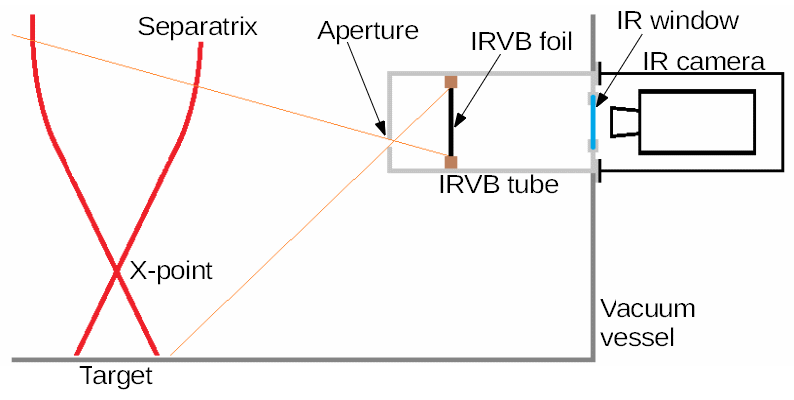
\includegraphics[width=0.7\linewidth]{Chapters/chapter2/figs/IRVB cartoon.png}
	\caption{Schematic representation of the main components of a IRVB diagnostic}
	\label{fig:IRVB_sketch}
\end{figure}

There are various elements to consider in the design of the IRVB diagnostic as shown in \autoref{fig:IRVB_sketch}.
Considering how thin a typical carbon coated foil is (composed of $10\mu m$ graphite + $2.5\mu m$ platinum + $10\mu m$ graphite as per \cite{Pandya2014} and their standard properties), when the temperature on one side is increased by a set amount it takes $\sim7ns$ for the other side to reach the 99\% of that increase. The heat transfer across the foil is so fast compared to the maximum frame rate of the infrared (IR) cameras available (tens of kHz) and the timescale of the phenomena of interest (1-10ms) that it permits treating heat diffusion as a 2D problem. The thinner the foil the lower the thermal inertia, allowing for a higher temperature rise for given input power. The thickness must nevertheless be large enough for the vast majority of the radiation to be absorbed. The foil must also (if a significant amount of neutrons are produced by the plasma) be made of a material weakly prone to neutron induced transmutation and vacuum compatible.\cite{Mukai2021}
It is important that the foil has low reflectivity for the wavelength range of interest. Metals normally used in bolometers have low reflectivity for UV and shorter wavelengths, but high for longer as the majority of radiation from the plasma is emitted at VUV wavelengths. This is usually addressed by coating the foil with a thin layer of carbon (as done in our case), known as "blackening", that weakly absorbs and weakly reflects high energy photons but has low reflectivity and high absorption at low energies. The coating does not significantly impact the reflectivity of radiation entering the diagnostic at shallow angles and reaching the foil supports.\cite{Gullikson2022} This light would require multiple reflections to reach the foil and would, therefore, be scattered resulting in a weak offset in a large portion of the foil. This would not change its capability to observe sharp features from the plasma. The coating introduces an interface between materials that might impede heat transfer and increases the mass of the foil increasing its inertia. The coating could also, depending on the technique, be deposited non uniformly on the foil, adding to the non uniformity already present on the foil. The coating must also be stable and vacuum compatible.\cite{Mukai2016}

The infrared camera must be positioned as close as possible to the foil in order to increase the resolution and signal to noise ratio. If the neutron flux is significant, or there are mechanical constraints, mirrors or periscopes must be used. All apparatus must be suitable to transmit infrared radiation and properly coated to avoid reflections. The camera itself has to be suitable for measuring temperature differences of few K around room or vacuum vessel temperature.
Of great importance in the design is the positioning and size of the pinhole aperture with respect of the foil. The distance and position impacts the field of view (FOV) of the diagnostic, its spatial resolution and the radiation intensity.

\section{MAST-U IRVB design}\label{MAST-U IRVB design}
The entire IRVB hardware design and optimisation was originally done by Matthew Reinke, based on work previously done for NSTX-U.\cite{VanEden2016} The definition of the materials, verification of compatibility with MAST-U vacuum and magnetic environment, procurement as well as the initial training of the author on the calibration and assembly of an IRVB system was by Reinke. The design was then verified and confirmed by the author with the selection of the fine tuning hardware feature mentioned in this section.

Here it will be shown how the design was adapted to the specific geometry of MAST-U.
The vertical location of the IRVB was dictated by the available ports on the machine. The one assigned to the IRVB is HE11-2, located in sector 11 and centered $0.7m$ below the midplane. The pinhole was placed as close as possible to the plasma to enable an unobstructed, wide field of view while being protected by the surrounding structures and safely outside the plasma scrape-off layer (SOL), at a radius of $1.55m$. The resulting positioning of the IRVB tube can be seen in \autoref{fig:IRVB_location}. 

\begin{figure}[!ht]
	\centering
	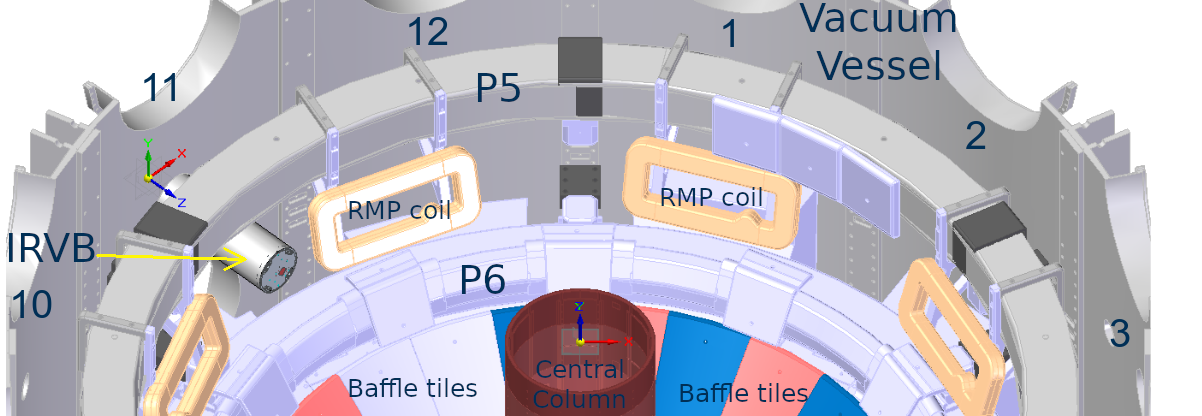
\includegraphics[trim={7 0 60 0},clip,width=0.8\linewidth]{Chapters/chapter2/figs/where_irvb2.png}
	\caption{Top view of the lower half of MAST-U, showing the positioning of the IRVB inside the vacuum vessel respect to other features. The numbers identify the sectors, assigned clockwise in the toroidal direction.}
	\label{fig:IRVB_location}
\end{figure}

With the above constraints, the pinhole was located off the centre of the foil so that the the LOS starting from the x-point in the poloidal view of the plasma would land in the centre of the foil. Two-thirds of the foil surface will have a mostly poloidal view of the plasma, while one-third will have a mainly tangential view. The foil is composed of a $2.5\mu m$ platinum film coated with graphite on both sides of dimensions ${9\times7cm}$ as supplied by the National Institute for Fusion Science (NIFS), with the longer side aligned with the vertical axis of the machine to provide a large coverage in that direction. An exploded view of the components and their final appearance are shown in 
\autoref{fig:IRVB3} and \autoref{fig:IRVB_components} respectively.
In the design of the assembly, particular care was dedicated to:
\begin{enumerate}
    \item The presence on the re-entrant and air side section of the diagnostic of features that can be used to align the view with the MAST-U geometry as intended.
    \item The mechanical rigidity of the assembly and the increase of magnetic permeability due to welds. The tube has a weld along its length that was heat treated to reduce the relative magnetic permeability below 1.05.
    \item Blackening all the surfaces that could cause reflections and direct light to the foil. The entire detector sub-assembly was blackened with Moly-Paul powder in an isopropanol solution (the same used within the MAST-U vacuum vessel (VV)) while it was deemed sufficient to grit blast the other surfaces.
    \item The presence of cutouts in the tube to equalise the pressure within. The effect of rapid pressure changes was tested on a dummy foil created for this purpose in the benchtop setup (see \autoref{fig:vacuum_setup}) causing no motion of the foil with depressurization of up to $0.05bar/s$ (only cooling due to ambient air decompression) and visible motion but no damage up to $0.2bar/s$.
    \item Maintaining electrical isolation between the tube and the absorber assembly (foil and copper plates) with PEEK isolation washers to avoid eddy currents through the absorber.
    \item Use of vented screws for tapped holes to avoid trapping air and slowing down the vessel pump down.
\end{enumerate}

\begin{figure*}
	\centering
	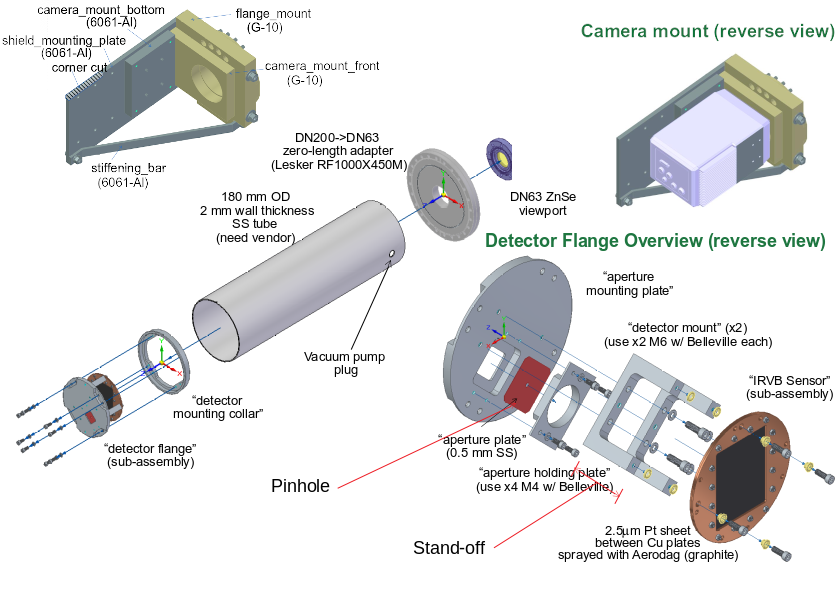
\includegraphics[trim={0 0 0 0},clip,width=\linewidth]{Chapters/chapter2/figs/IRVB3.png}
     \caption{IRVB components overview: exploded view showing all internal components before welding and assembly.}
     \label{fig:IRVB3}
\end{figure*}

         
\begin{figure}[!ht]
     \begin{subfigure}{0.49\linewidth}
         \centering
         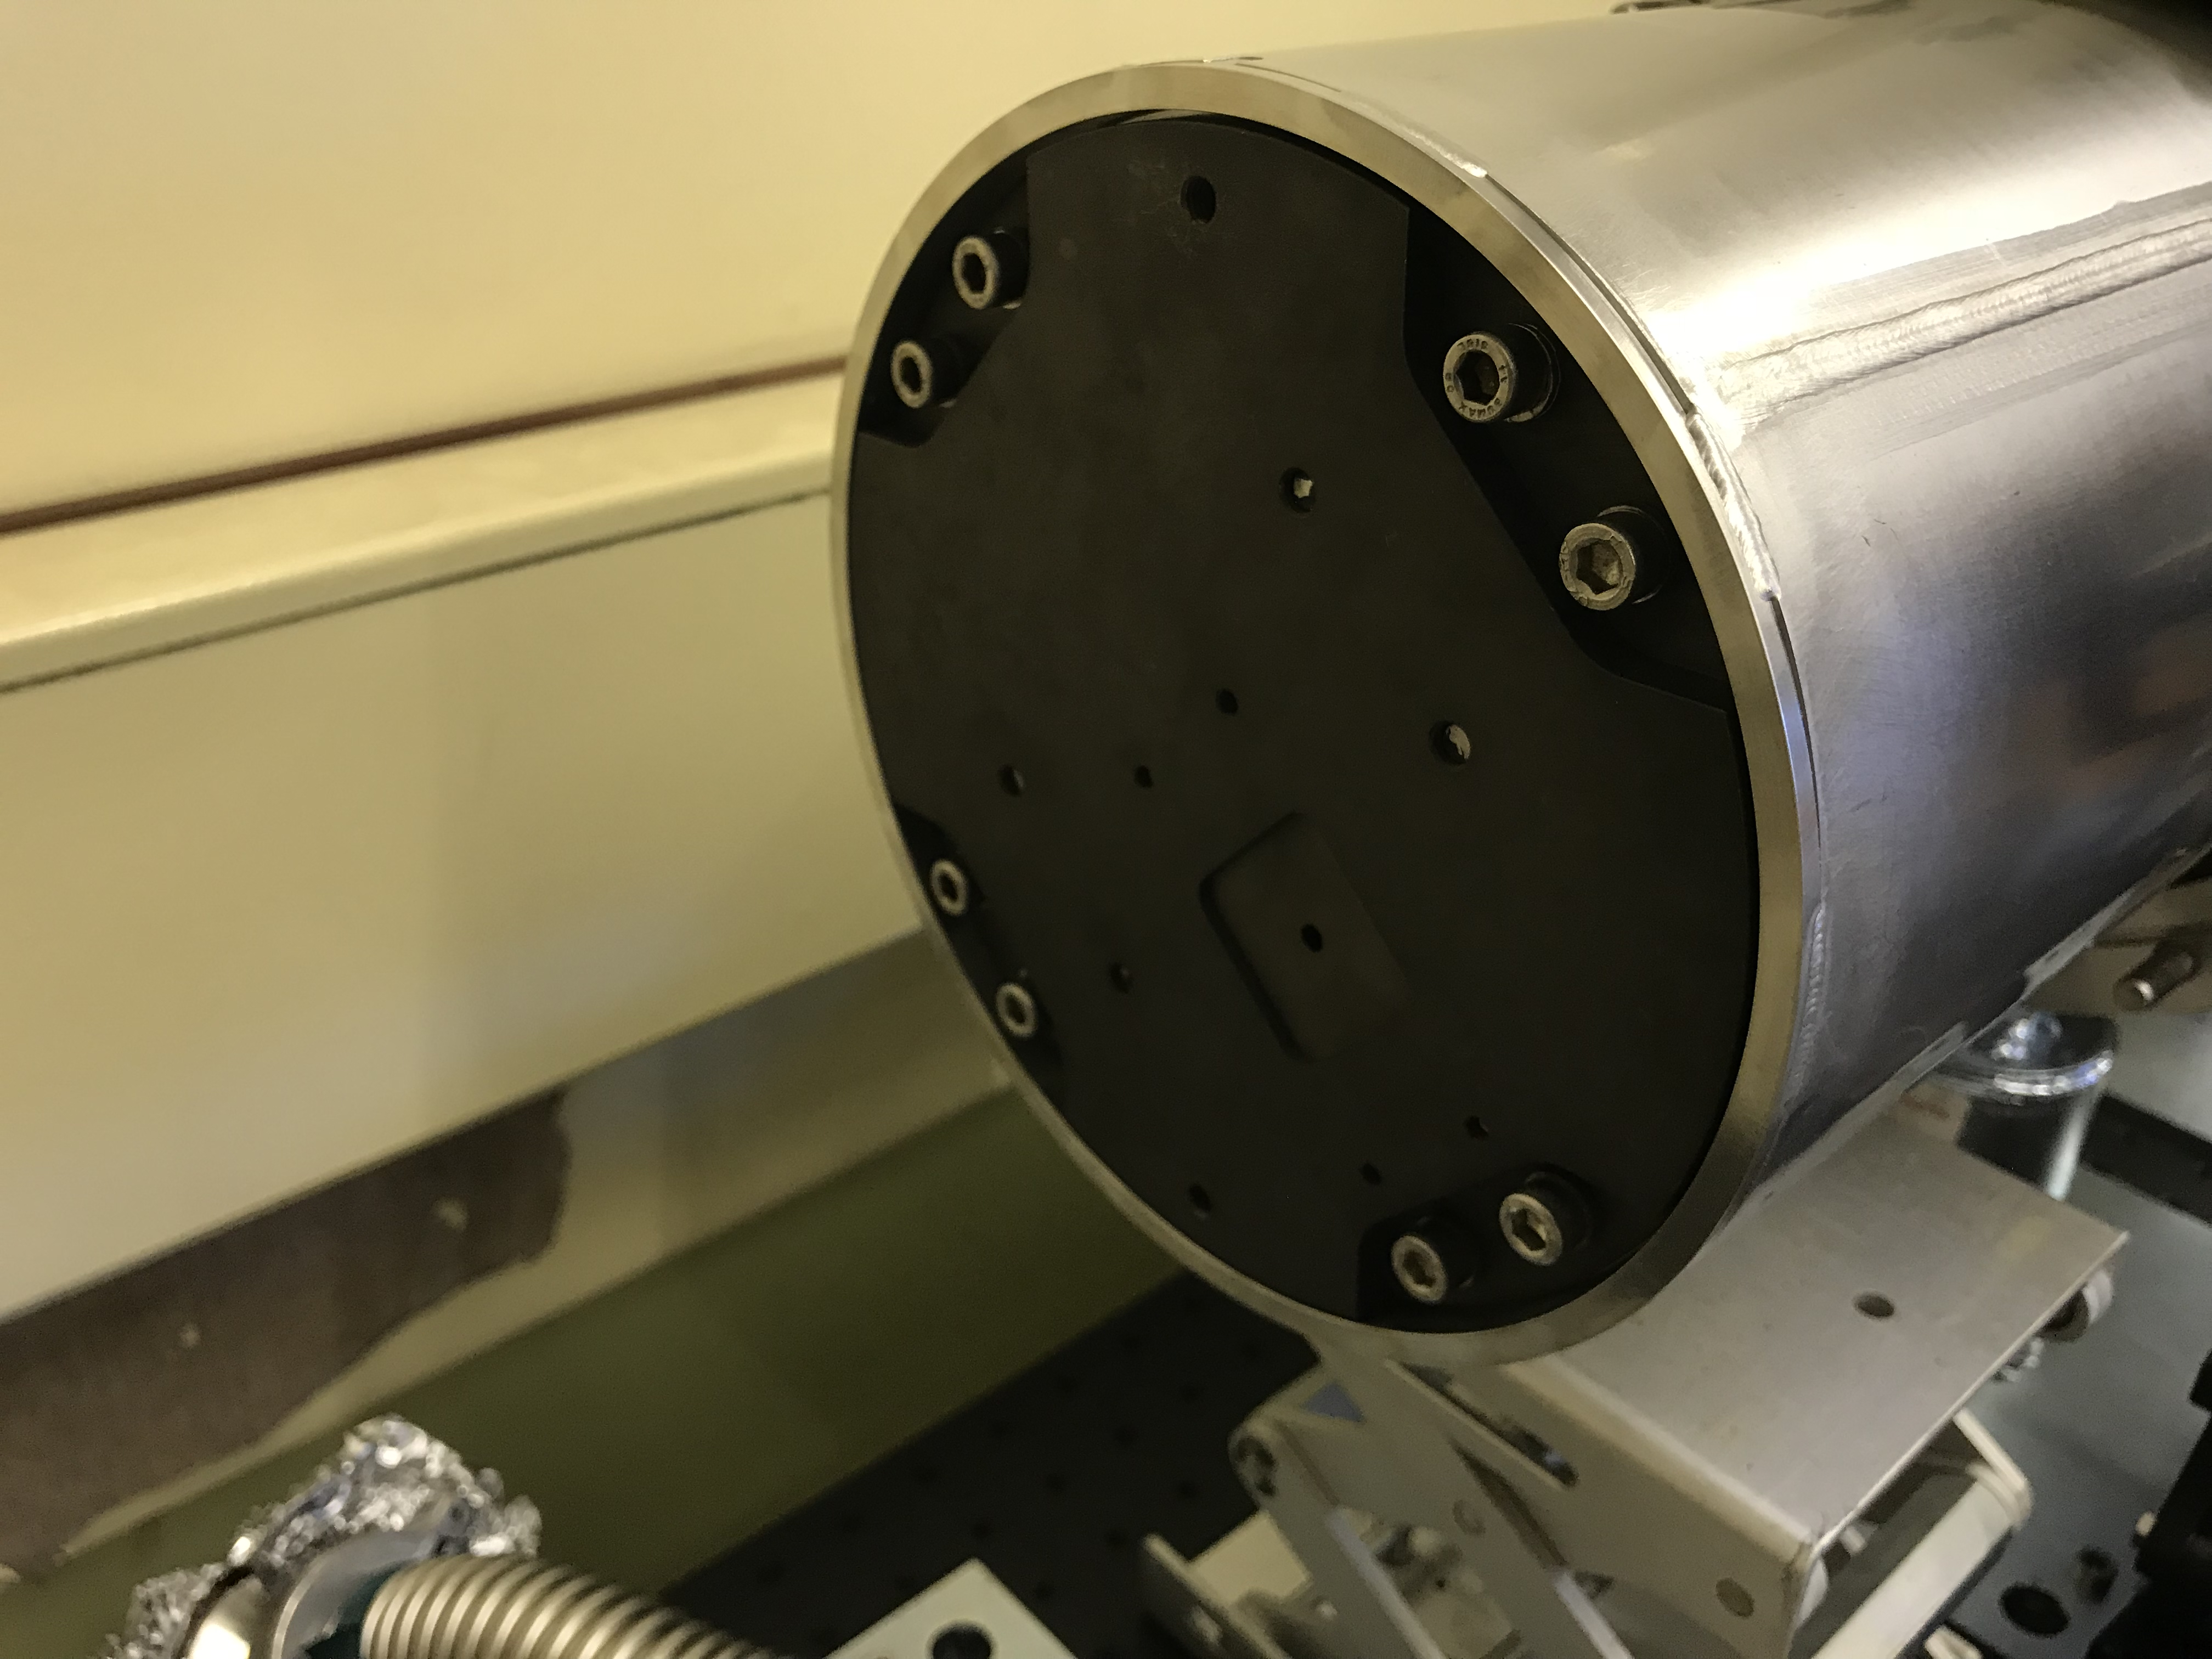
\includegraphics[trim={1500 500 0 0},clip,width=\textwidth]{Chapters/chapter2/figs/2018-07-23 11.25.01.jpg}
         \caption{}
         \label{fig:IRVB4}
     \end{subfigure}
     \begin{subfigure}{0.49\linewidth}
         \centering
         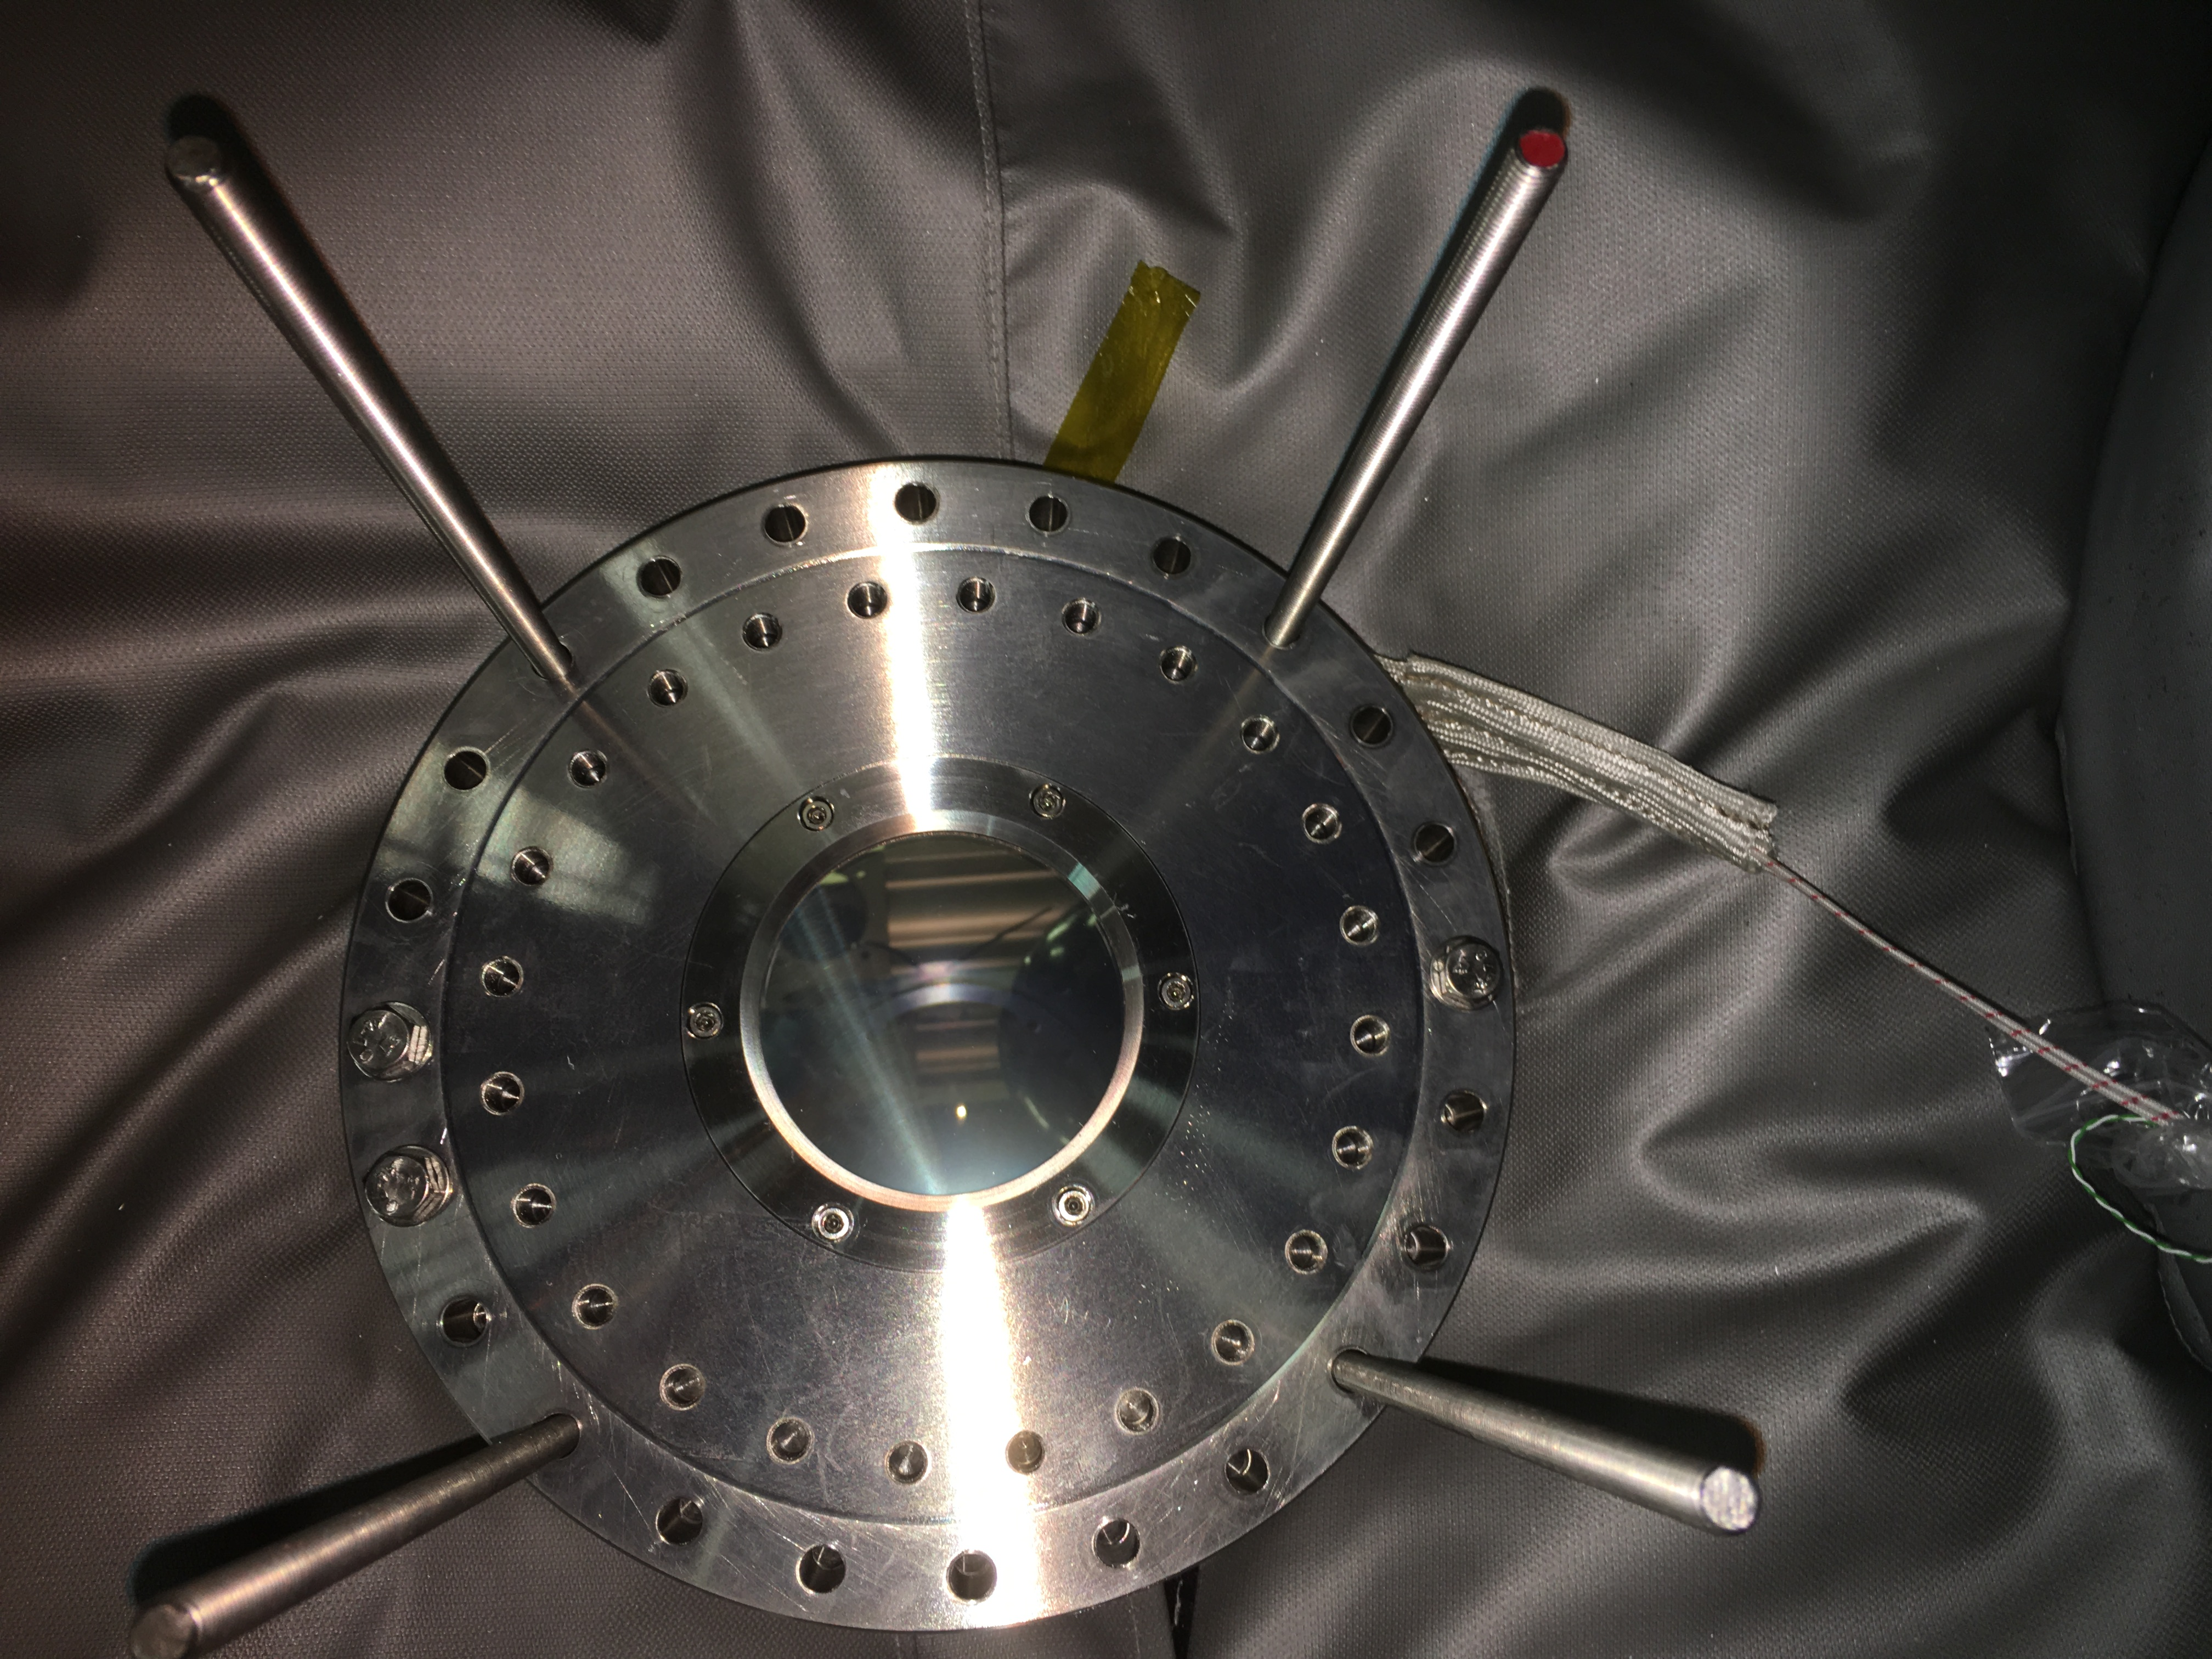
\includegraphics[trim={500 0 1000 500},clip,width=\textwidth]{Chapters/chapter2/figs/IMG_7199.JPG}
         \caption{}
         \label{fig:IRVB5}
     \end{subfigure}
     \centering
     \begin{subfigure}{0.8\linewidth}
         \includegraphics[trim={0 500 0 700},clip,width=\textwidth]{Chapters/chapter2/figs/IMG_20210514_121600812.jpg}
         \caption{}
         \label{fig:IRVB6}
     \end{subfigure}

    \caption{IRVB components overview: (\subref{fig:IRVB4}) photograph of the exterior of the foil assembly inside the tube, (\subref{fig:IRVB5}) the view port side of the tube installed in MAST-U and (\subref{fig:IRVB6}) the camera installed on the flange respectively. Photographs taken 2018/07/23, 2018/12/03, 2021/05/14 respectively. To change pinhole size and foil pinhole distance the tube must be removed while the camera is always accessible.}
    \label{fig:IRVB_components}
\end{figure}

The power density on the foil was estimated with CHERAB \cite{C.GiroudA.MeakinsM.CarrA.Baciero2018,Carr2017,A.MeakinsCarrM.2017}, a code that can perform ray tracing with the full geometry of MAST-U. Based on prior experience with the IRVB on NSTX-U\cite{Reinke2018}, the noise equivalent power density (NEPD) is expected to be in the region of $\sim5 W/m^2$, and so a desired signal of $\sim100 W/m^2$ was utilized in the pinhole camera design. 3 possible pinhole diameter sizes have been evaluated in order to tune the signal strength and resolution: 4, 6, 8 mm. In order to tune the magnification of the system 3 possible lengths of the bracket that connects the foil assembly to the pinhole one (the stand-off) have been considered: 45, 60, 75 mm. The result from the simulations for the 9 combination of configurations is shown in \autoref{fig:cherab1}.\cite{Federici2022} The stand-off distances of 60 and 75cm allow the entire foil to observe the plasma and not be obscured by coils. With a 75cm stand-off both a smaller fraction of the SXD chamber and of the outer leg in the tangential view (right side of the foil) would be out the FOV. Pinhole diameters of 6 and 8mm return a much larger signal than the desired minimum of $100 W/m^2$. In \autoref{fig:pinhole_resolution} it is illustrated how, with a smaller pinhole, the signal level is lower but it is easier to identify close but distinct structures in the radiation distribution, even from the poloidal view alone (left side of the foil). For closer radiating structures it would be easier to distinguish them as separate in the tangential view  with a smaller rather than large pinhole. For these reasons, the configuration that includes in the FOV the features of interest and allows for the highest spatial resolution, while maintaining a sufficiently high SNR, is a stand-off of 60cm and pinhole diameter of 4mm.

\begin{figure}[!ht]
     \centering
     \begin{subfigure}{0.31\textwidth}
         \centering
         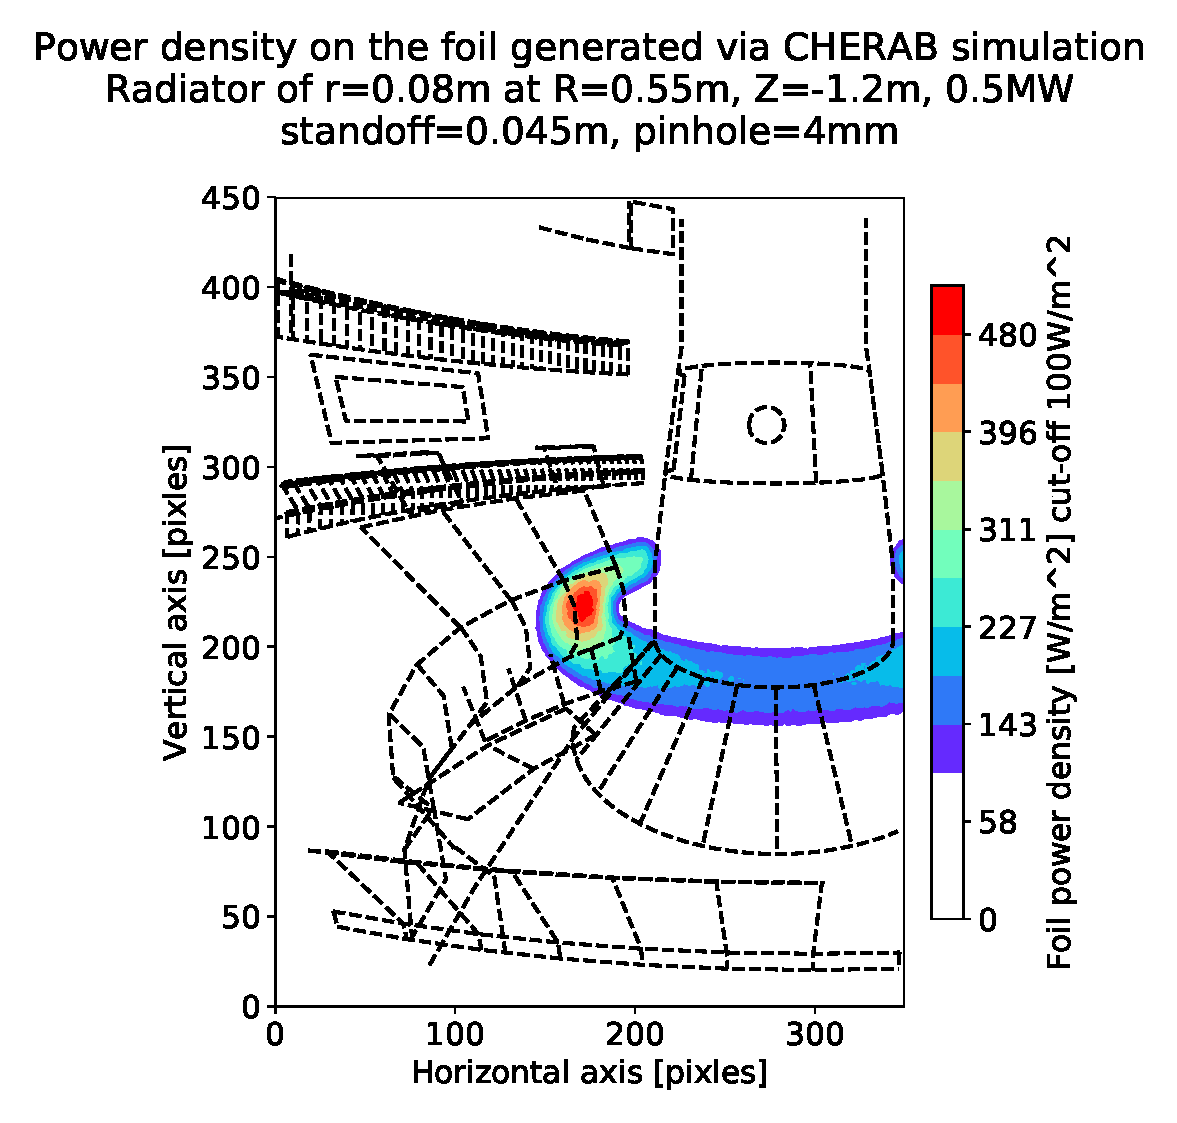
\includegraphics[trim={85 25 57 80},clip,width=\textwidth]{Chapters/chapter2/figs/measured_power_4_45radiator_R0.55_Z-1.2_r0.08.stl.eps}
         \caption{pinhole 4mm/stand-off 45mm}
         \label{fig:4_45}
     \end{subfigure}
     \hfill
     \begin{subfigure}{0.31\textwidth}
         \centering
         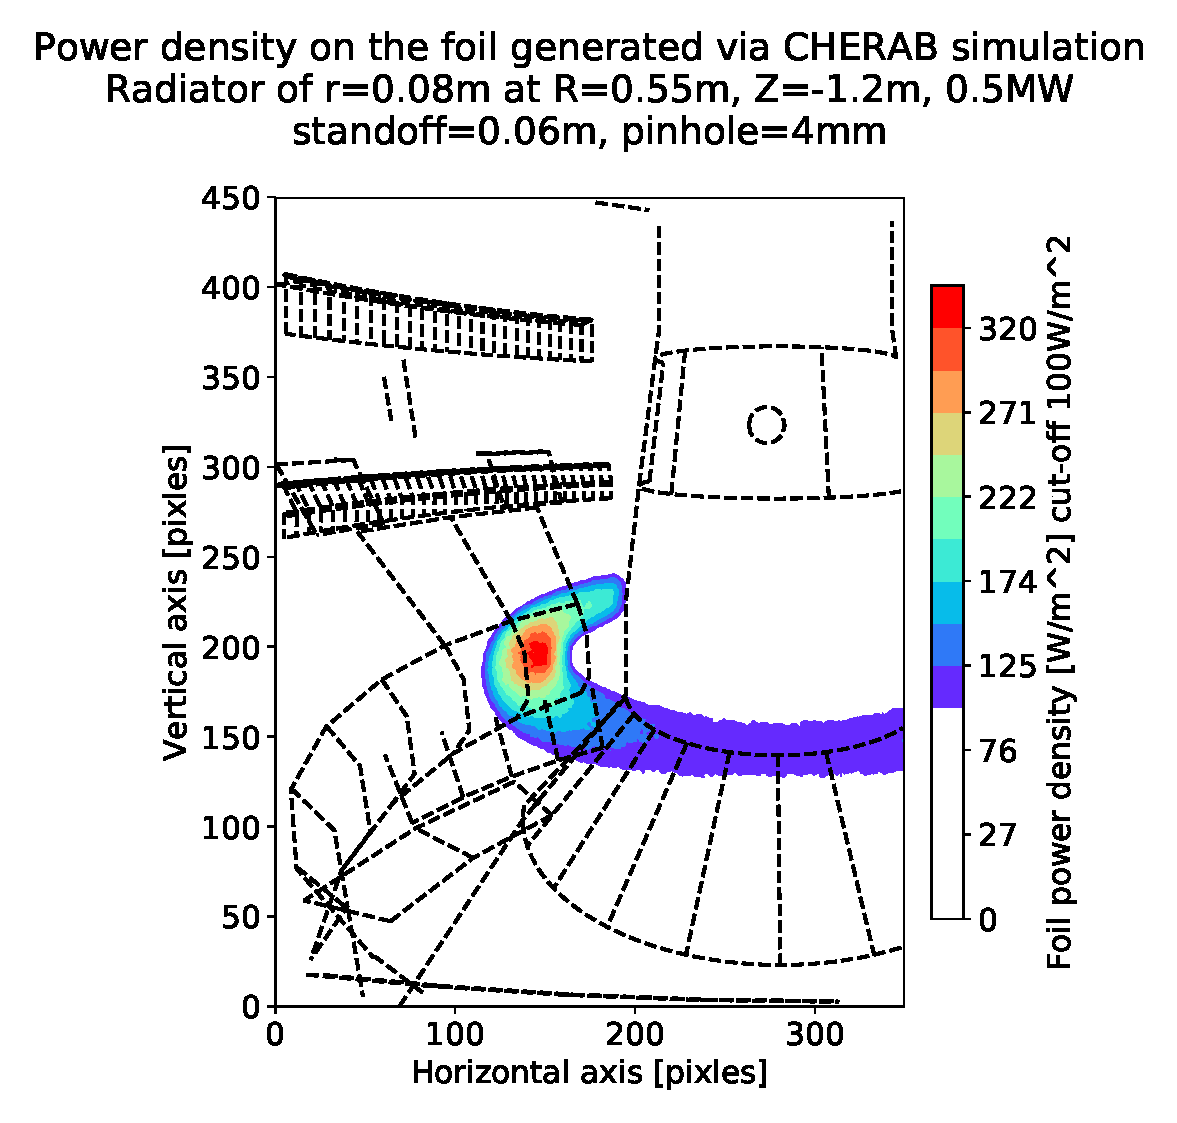
\includegraphics[trim={85 25 57 80},clip,width=\textwidth]{Chapters/chapter2/figs/measured_power_4_60radiator_R0.55_Z-1.2_r0.08.stl.eps}
         \caption{$4/60$}
         \label{fig:4_60}
     \end{subfigure}
     \hfill
     \begin{subfigure}{0.325\textwidth}
         \centering
         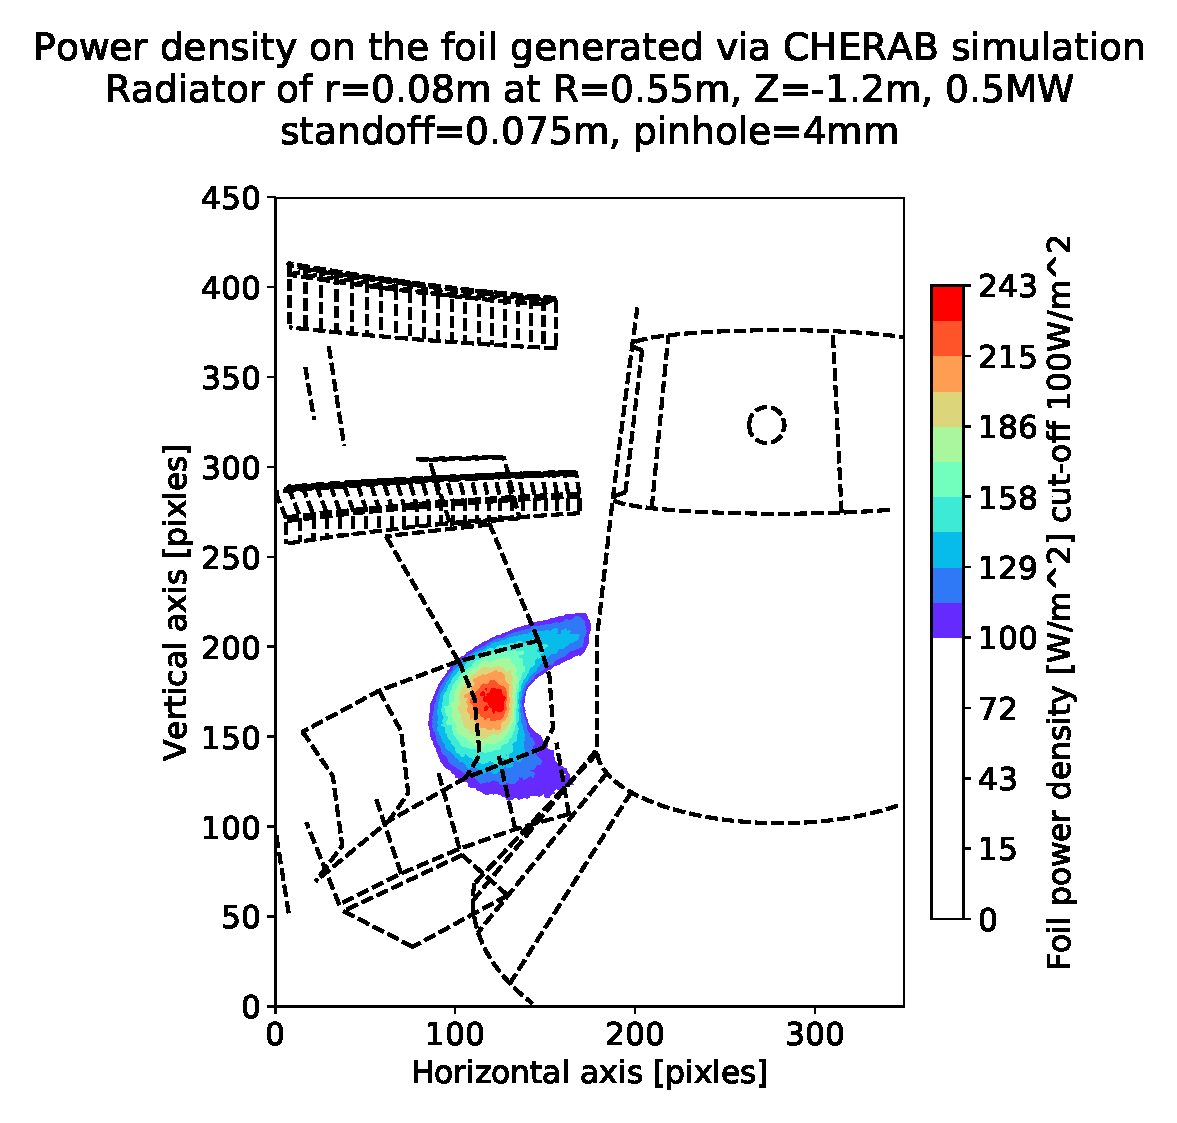
\includegraphics[trim={85 25 40 80},clip,width=\textwidth]{Chapters/chapter2/figs/measured_power_4_75radiator_R0.55_Z-1.2_r0.08.stl.eps}
         \caption{$4/75$}
         \label{fig:$4_75$}
     \end{subfigure}
     \begin{subfigure}{0.32\textwidth}
         \centering
         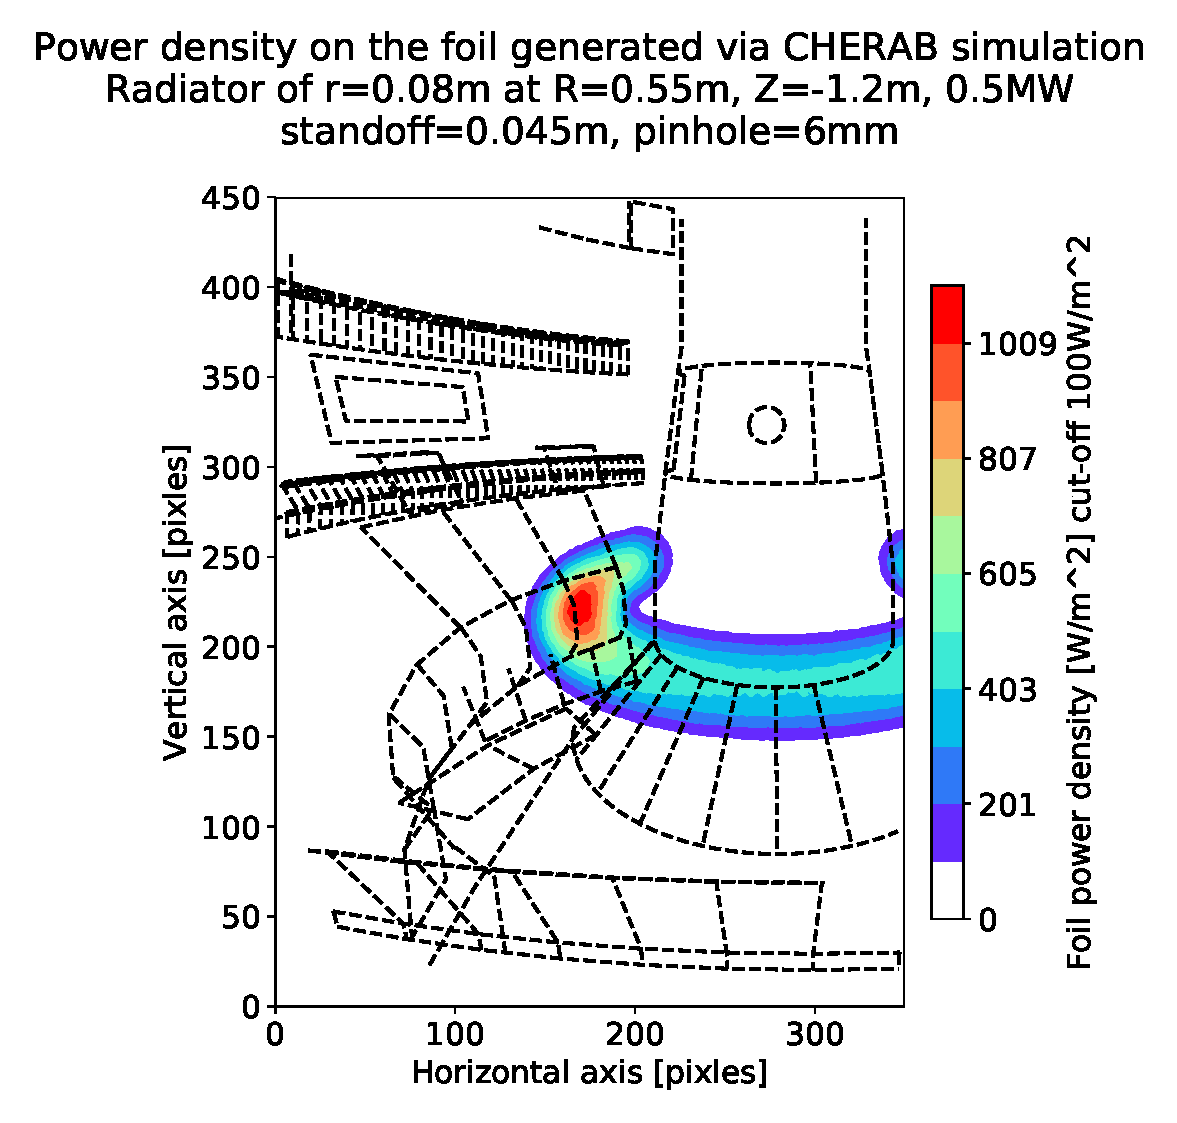
\includegraphics[trim={85 25 49 80},clip,width=\textwidth]{Chapters/chapter2/figs/measured_power_6_45radiator_R0.55_Z-1.2_r0.08.stl.eps}
         \caption{$6/45$}
         \label{fig:6_45}
     \end{subfigure}
     \hfill
     \begin{subfigure}{0.31\textwidth}
         \centering
         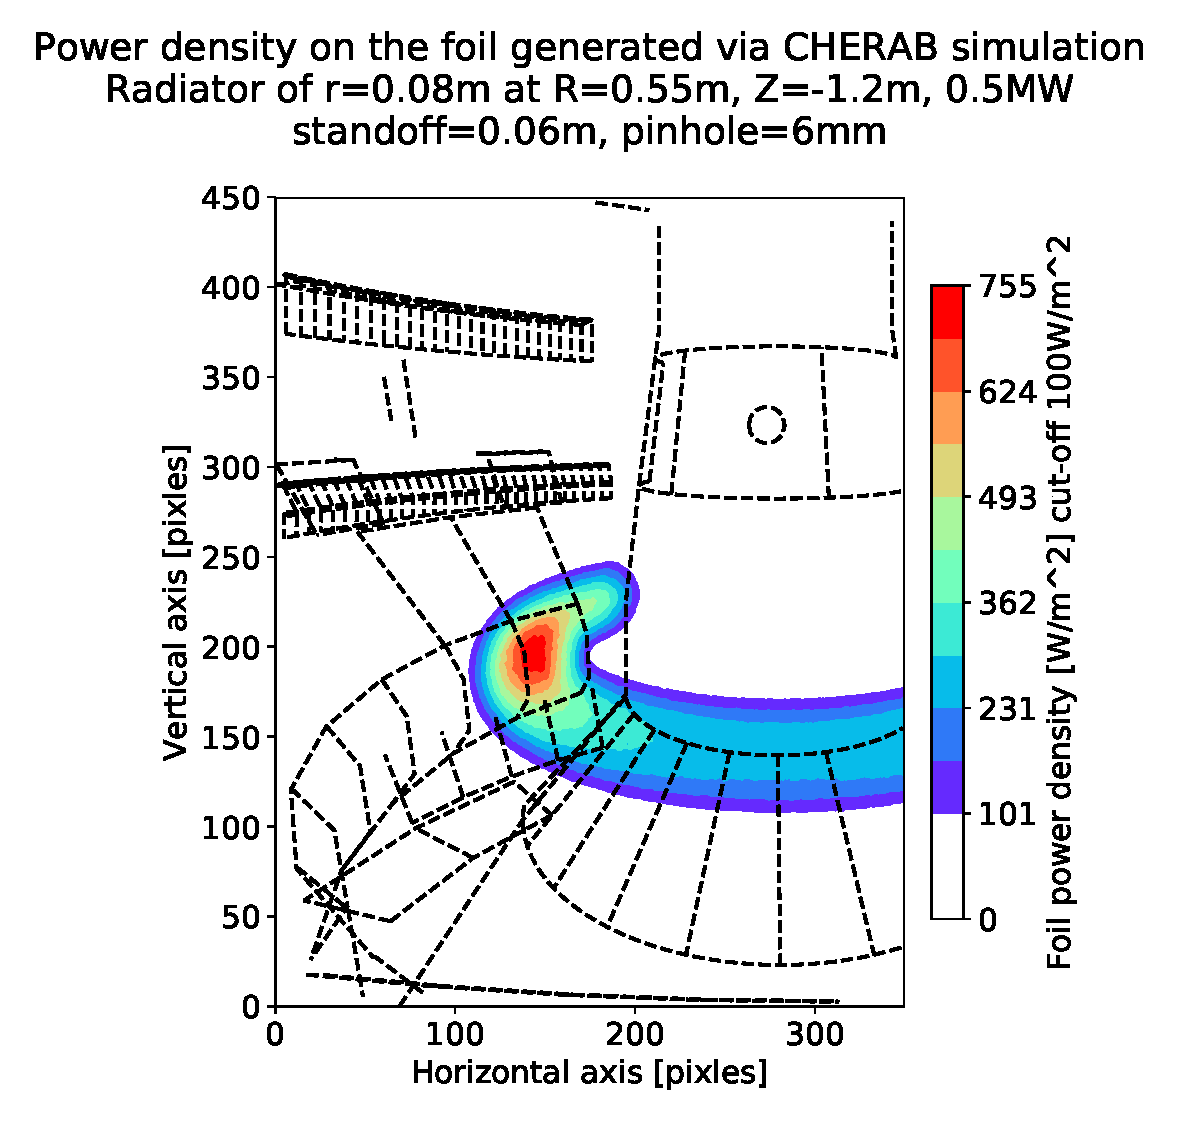
\includegraphics[trim={85 25 57 80},clip,width=\textwidth]{Chapters/chapter2/figs/measured_power_6_60radiator_R0.55_Z-1.2_r0.08.stl.eps}
         \caption{$6/60$}
         \label{fig:6_60}
     \end{subfigure}
     \hfill
     \begin{subfigure}{0.325\textwidth}
         \centering
         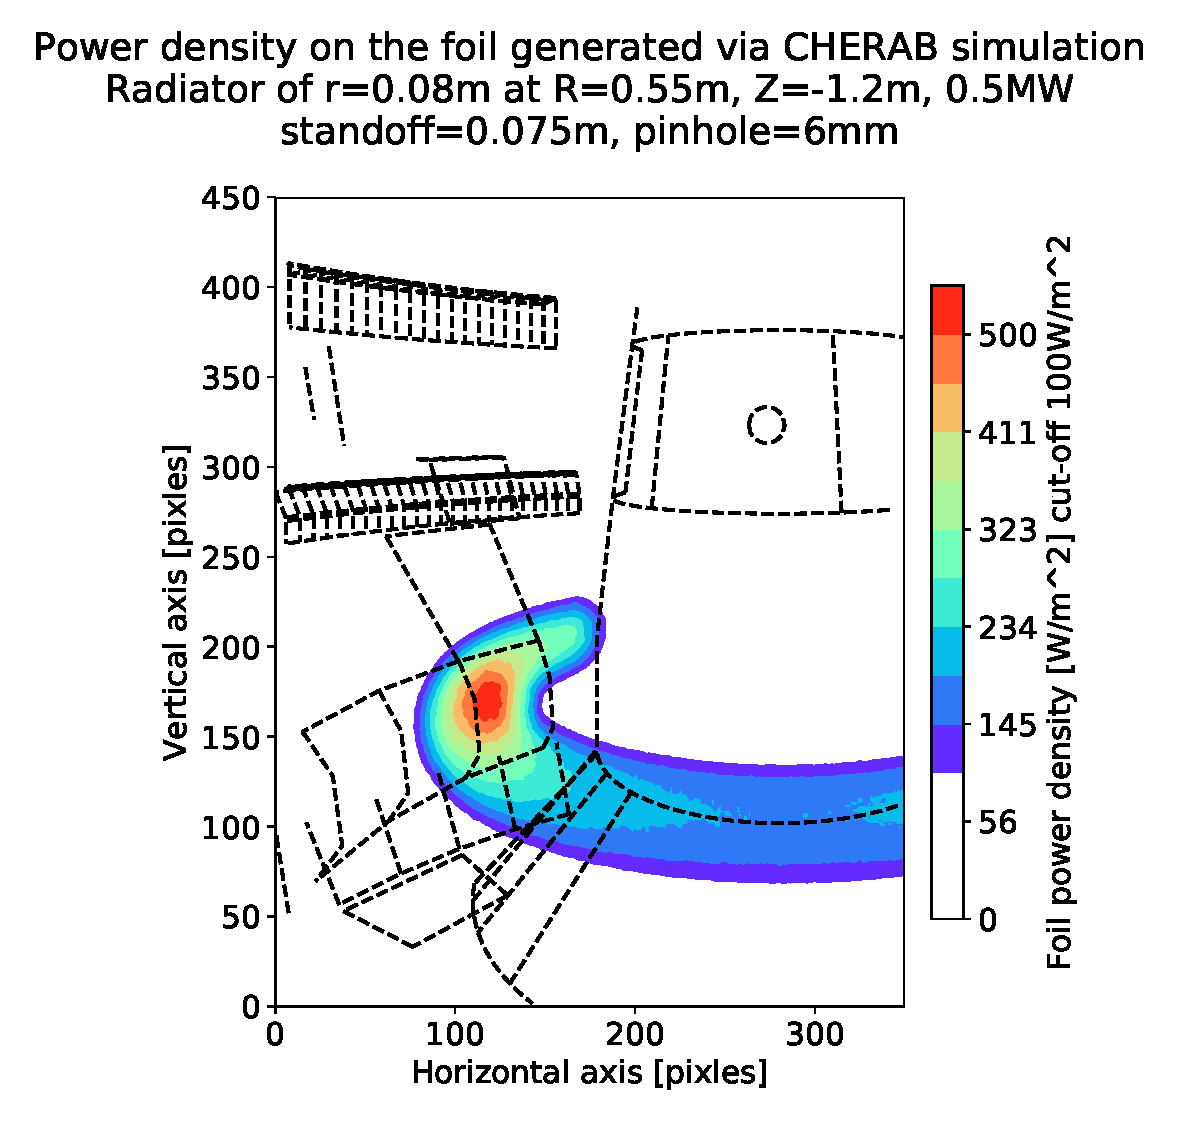
\includegraphics[trim={85 25 40 80},clip,width=\textwidth]{Chapters/chapter2/figs/measured_power_6_75radiator_R0.55_Z-1.2_r0.08.stl.eps}
         \caption{$6/75$}
         \label{fig:6_75}
     \end{subfigure}
     \begin{subfigure}{0.32\textwidth}
         \centering
         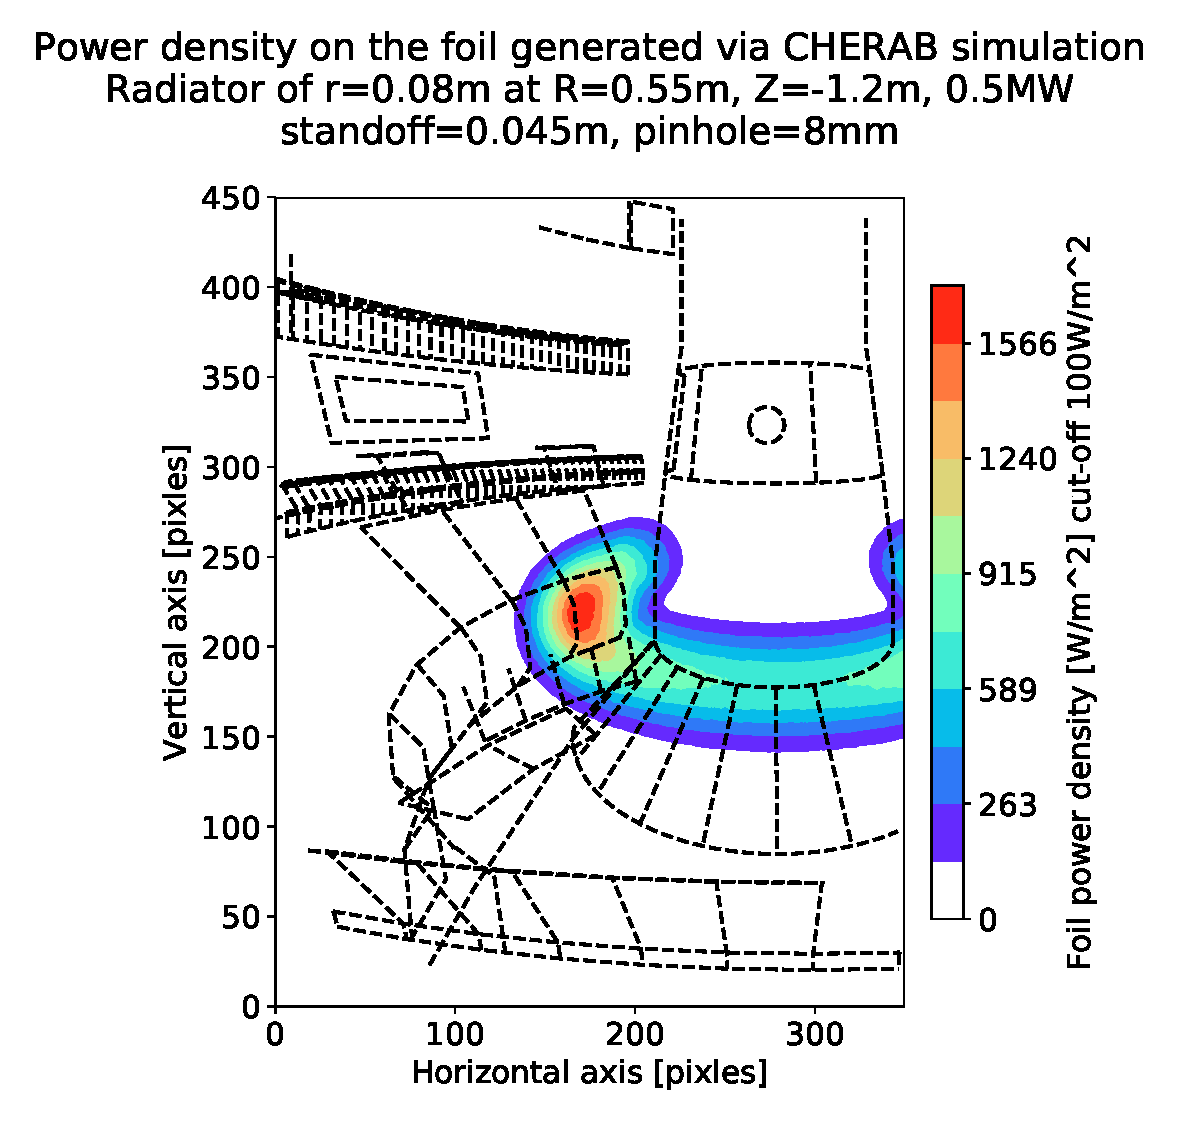
\includegraphics[trim={85 25 49 80},clip,width=\textwidth]{Chapters/chapter2/figs/measured_power_8_45radiator_R0.55_Z-1.2_r0.08.stl.eps}
         \caption{$8/45$}
         \label{fig:8_45}
     \end{subfigure}
     \hfill
     \begin{subfigure}{0.32\textwidth}
         \centering
         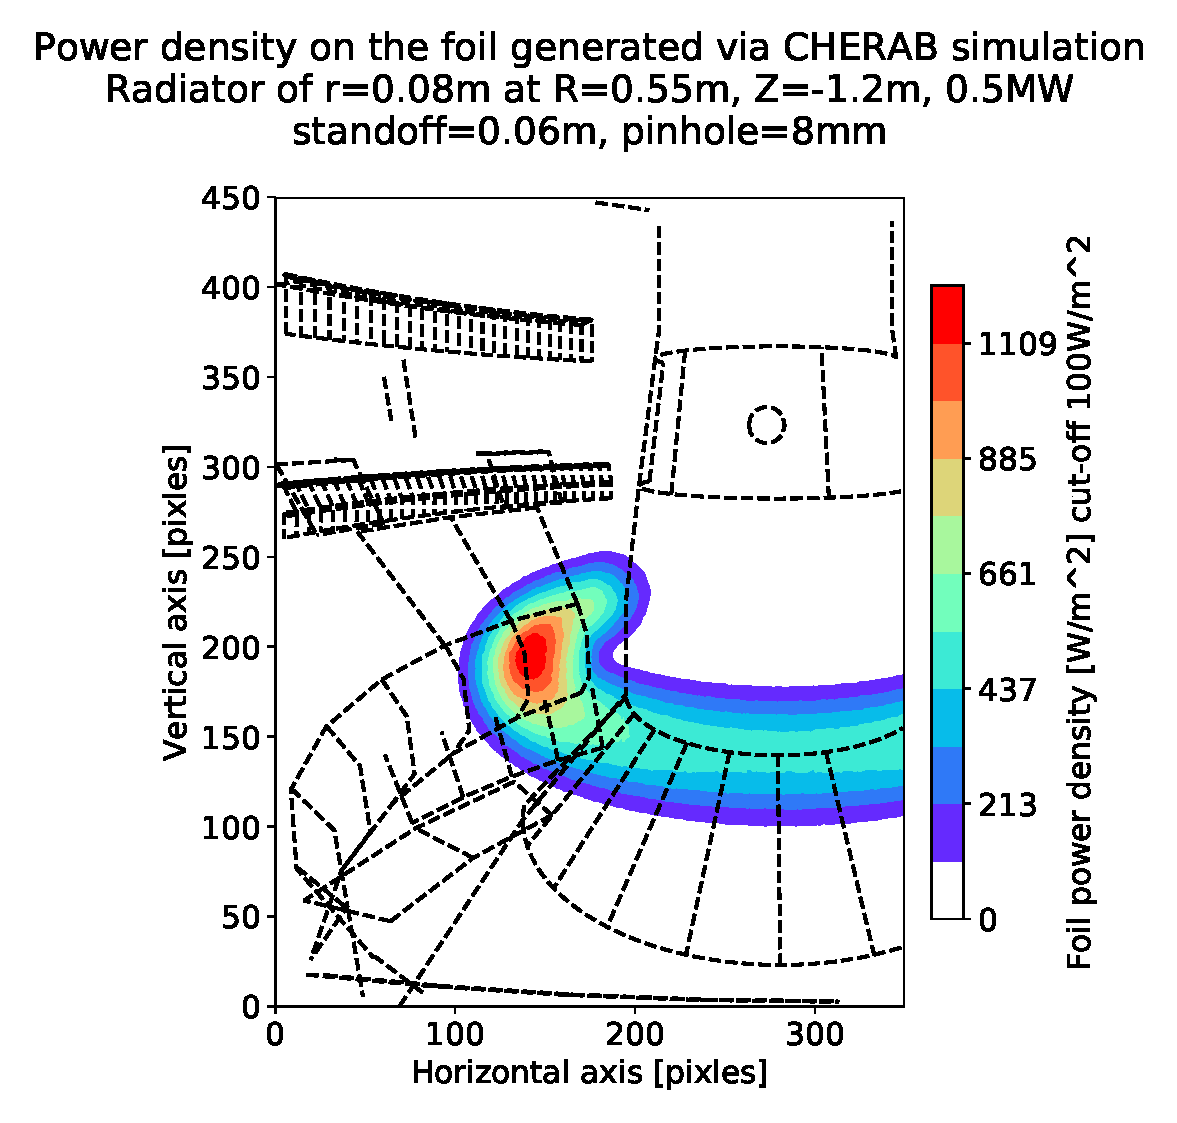
\includegraphics[trim={85 25 49 80},clip,width=\textwidth]{Chapters/chapter2/figs/measured_power_8_60radiator_R0.55_Z-1.2_r0.08.stl.eps}
         \caption{$8/60$}
         \label{fig:8_60}
     \end{subfigure}
     \hfill
     \begin{subfigure}{0.325\textwidth}
         \centering
         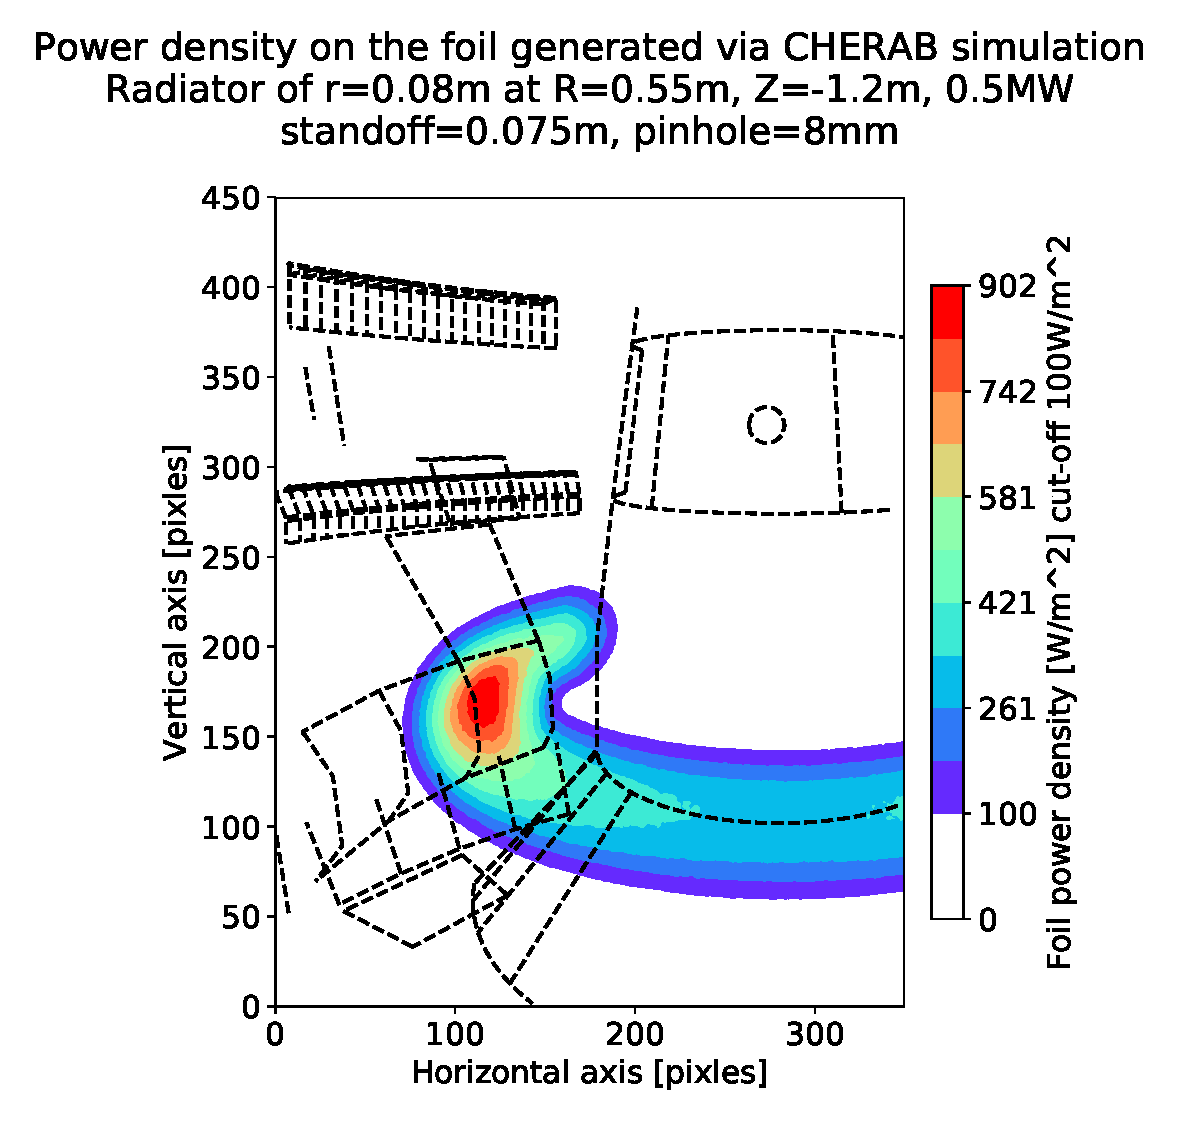
\includegraphics[trim={85 25 40 80},clip,width=\textwidth]{Chapters/chapter2/figs/measured_power_8_75radiator_R0.55_Z-1.2_r0.08.stl.eps}
         \caption{$8/75$}
         \label{fig:8_75}
     \end{subfigure}

    \caption{Radiated power deposited on foil from a homogeneous toroidal emitter of radius 8cm located at R=0.55m and Z=-1.2m, emitting a total of 0,5MW for the combinations of pinhole diameter and stand-off length considered. The power deposited on the foil below $100W/m^2$ is not shown, as that is the minimum desired signal level. In black are overlaid the projection of relevant features of MAST-U structure on the foil for reference.}
    \label{fig:cherab1}
\end{figure}

\begin{figure}[!ht]
     \centering
     \begin{subfigure}{0.7\linewidth}
         \centering
         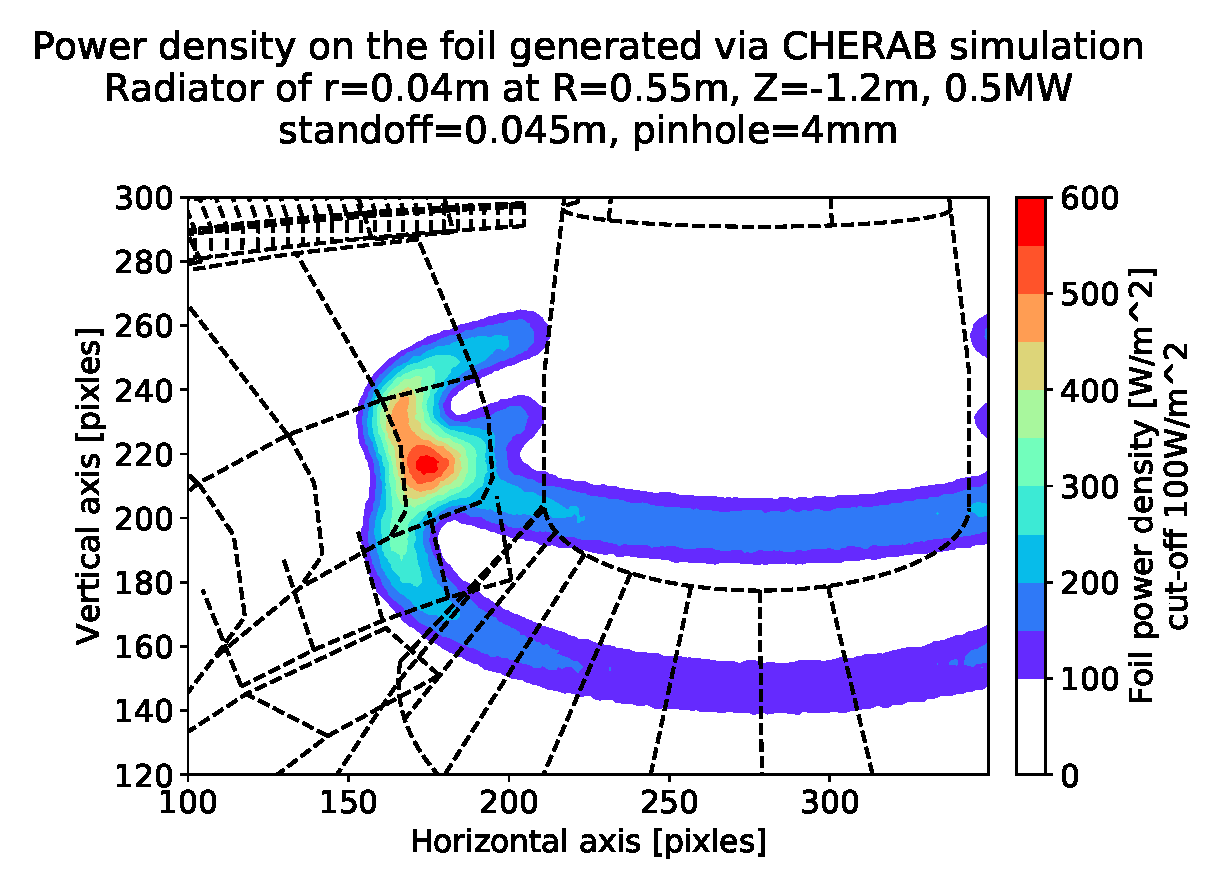
\includegraphics[trim={45 22 0 80},clip,width=\textwidth]{Chapters/chapter2/figs/measured_power_4_452x_radiator_R0.55_Z-1.2-1.3_r0.04.stl.eps}
         \caption{}
         \label{fig:pinhole_resolution4}
     \end{subfigure}
     \begin{subfigure}{0.7\linewidth}
         \centering
         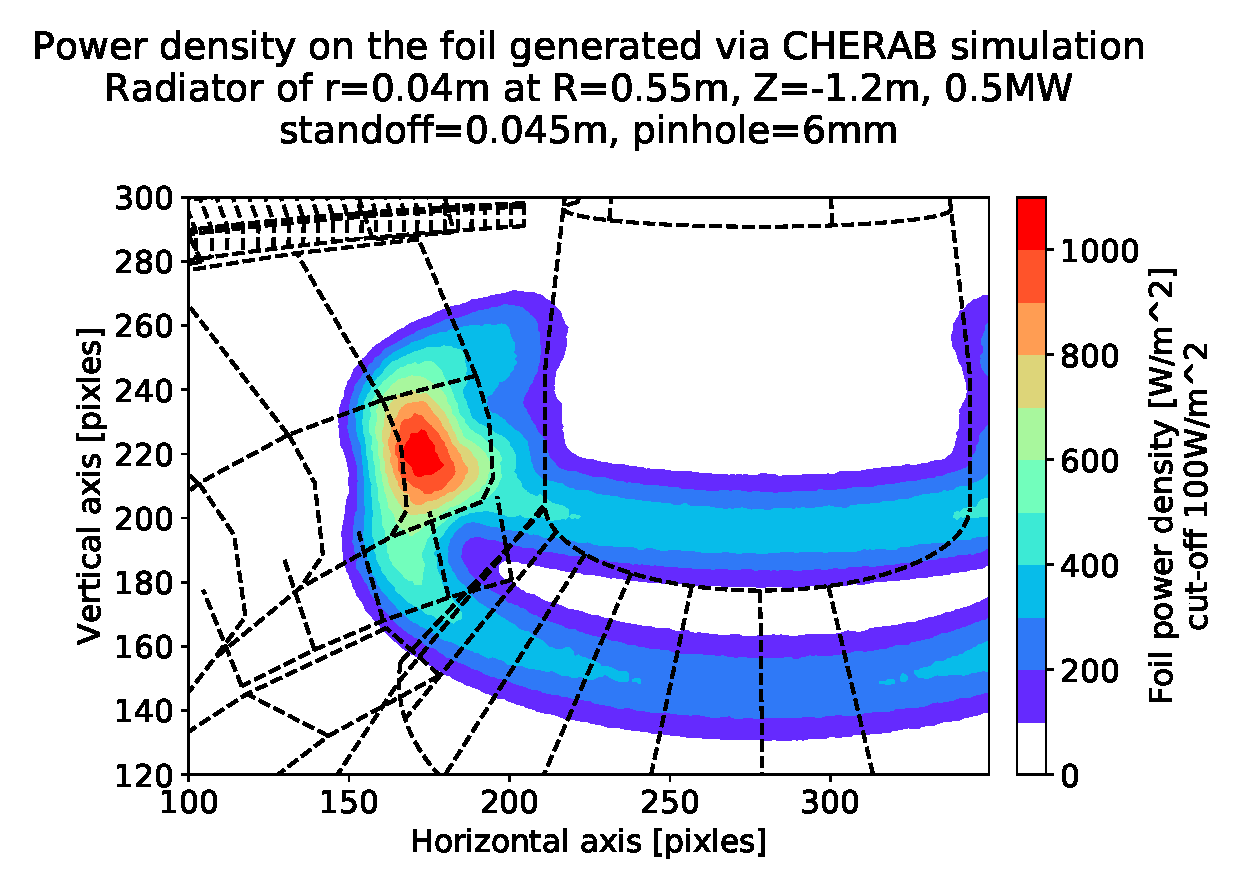
\includegraphics[trim={45 22 0 80},clip,width=\textwidth]{Chapters/chapter2/figs/measured_power_6_452x_radiator_R0.55_Z-1.2-1.3_r0.04.stl.eps}
         \caption{}
         \label{fig:pinhole_resolution6}
     \end{subfigure}
	\caption{Radiated power deposited on foil, modeled with CHERAB, of two toruses of 4 cm minor radius separated by 16cm in vertical position with uniform emissivity such as to total 0.5MW of radiated power, located at the expected x-point location. The pinhole size was varied from 4mm (\subref{fig:pinhole_resolution4}) to 6mm (\subref{fig:pinhole_resolution6}) to illustrate the loss of spatial resolution. The power deposited on the foil below $100W/m^2$ is not shown, as that is the minimum desired signal level. Only the relevant section of the foil is shown. In black are overlaid the projection of relevant features of MAST-U structure on the foil for reference.}
    \label{fig:pinhole_resolution}
\end{figure}

The power distribution on the foil was also simulated in the case of a core and divertor region filled with a homogeneous emitter, see \autoref{fig:cherab2}.
\begin{figure}[!ht]
     \centering
     \begin{subfigure}{0.48\linewidth}
         \centering
         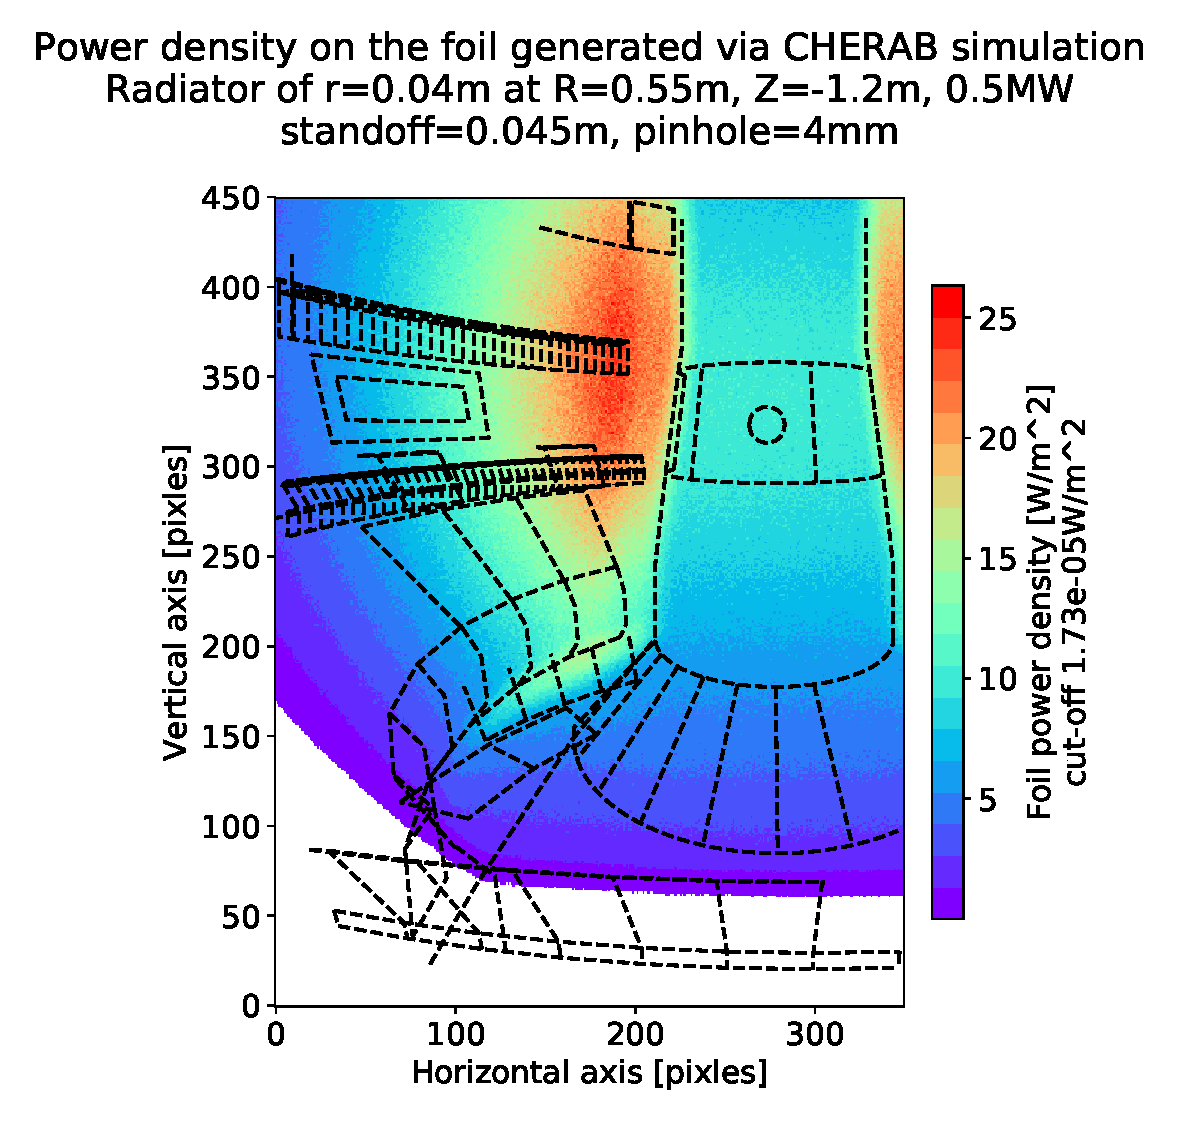
\includegraphics[trim={85 25 50 80},clip,width=\textwidth]{Chapters/chapter2/figs/measured_power_4_45radiator_all_core_and_divertor.stl.eps}
         \caption{pinhole 6mm/stand-off 45mm}
         \label{fig:4_45_all}
     \end{subfigure}
     \hfill
     \begin{subfigure}{0.48\linewidth}
         \centering
         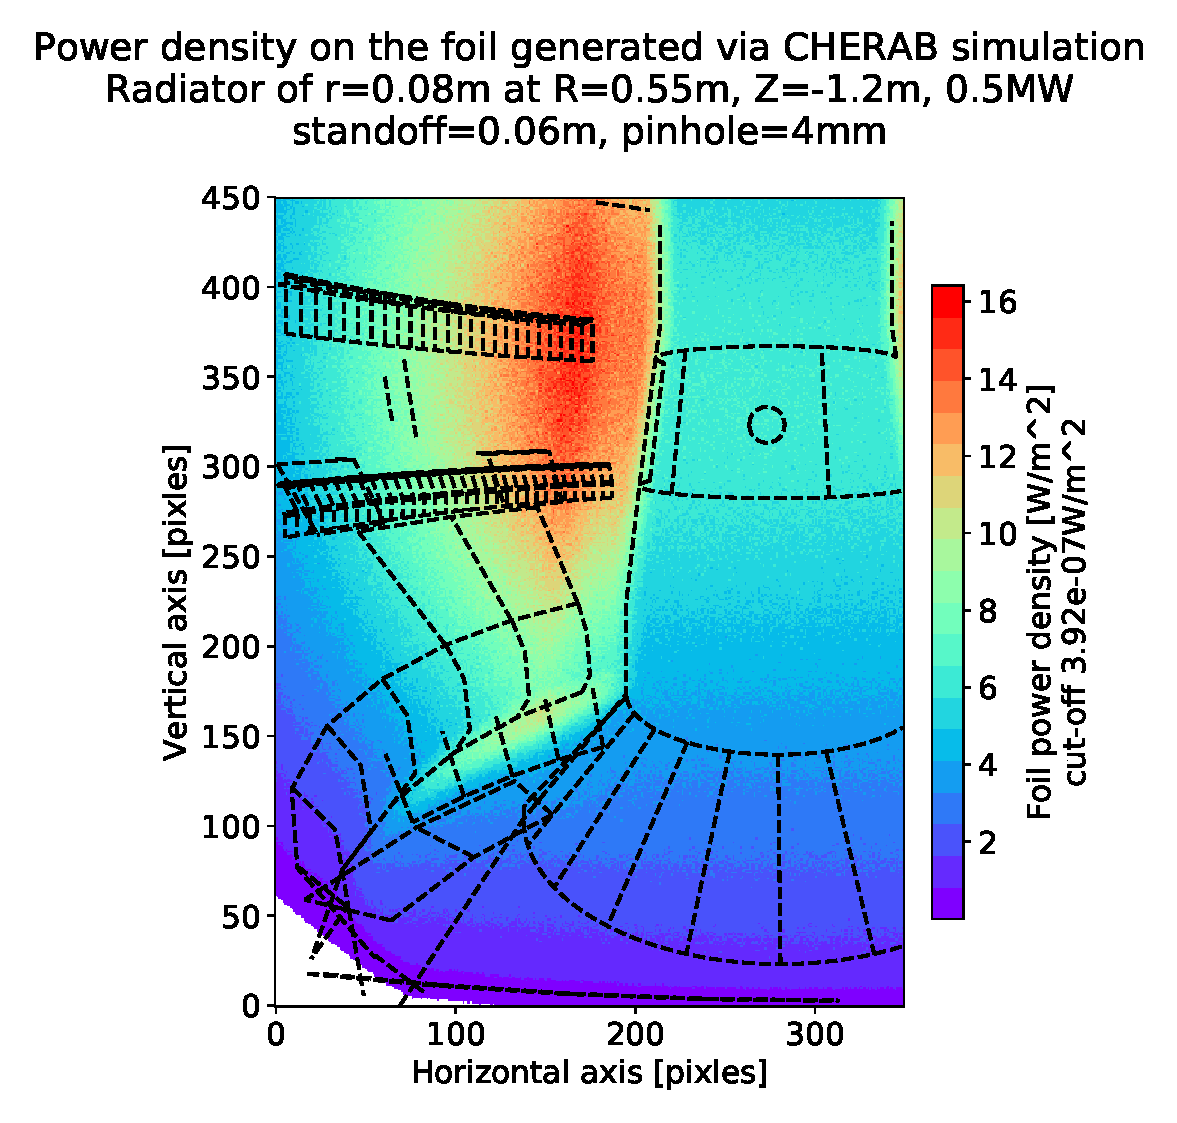
\includegraphics[trim={85 25 50 80},clip,width=\textwidth]{Chapters/chapter2/figs/measured_power_4_60radiator_all_core_and_divertor.stl.eps}
         \caption{$6/60$}
         \label{fig:4_60_all}
     \end{subfigure}

     \caption{Radiated power deposited on foil with a 4mm diameter pinhole and (\subref{fig:4_45_all}) 45mm and (\subref{fig:4_60_all}) stand-off between pinhole and foil, for the case of the core and divertor regions emitting homogeneously at a level of $50kW/m^3$. The white regions do not receive any radiation from the plasma, in black are overlaid the projection of relevant features of MAST-U structure on the foil for reference.}
    \label{fig:cherab2}
\end{figure}
The bottom left region of \autoref{fig:4_45_all} is where no radiation can arrive. This was helpful for the prototype phase, because that area could be used as a reference where the power is zero.
For this reason it has been decided to adopt a stand-off between pinhole and foil distance of 45mm for MU01, which covers the results shown in this work. This also returs an even larger radiation from the X-point. The MAST-U IRVB diagnostic has been returned to operation on MAST-U for the second campaign (MU02) with the optimal 60cm stand-off after re-evaluating the noise levels %(see \autoref{MU02 geometry optimisation}) 
and the spatial resolution achievable (see \autoref{chapter2.5}).

An approximate view inside MAST-U, imagining that the IRVB operates as a camera to show the features and obstructions, is shown in \autoref{fig:calcam}. The view of the plasma is mainly poloidal on the left side of the central column, but the field of view is large enough to see both sides of the central column.

\begin{figure}[!ht]
	\centering
	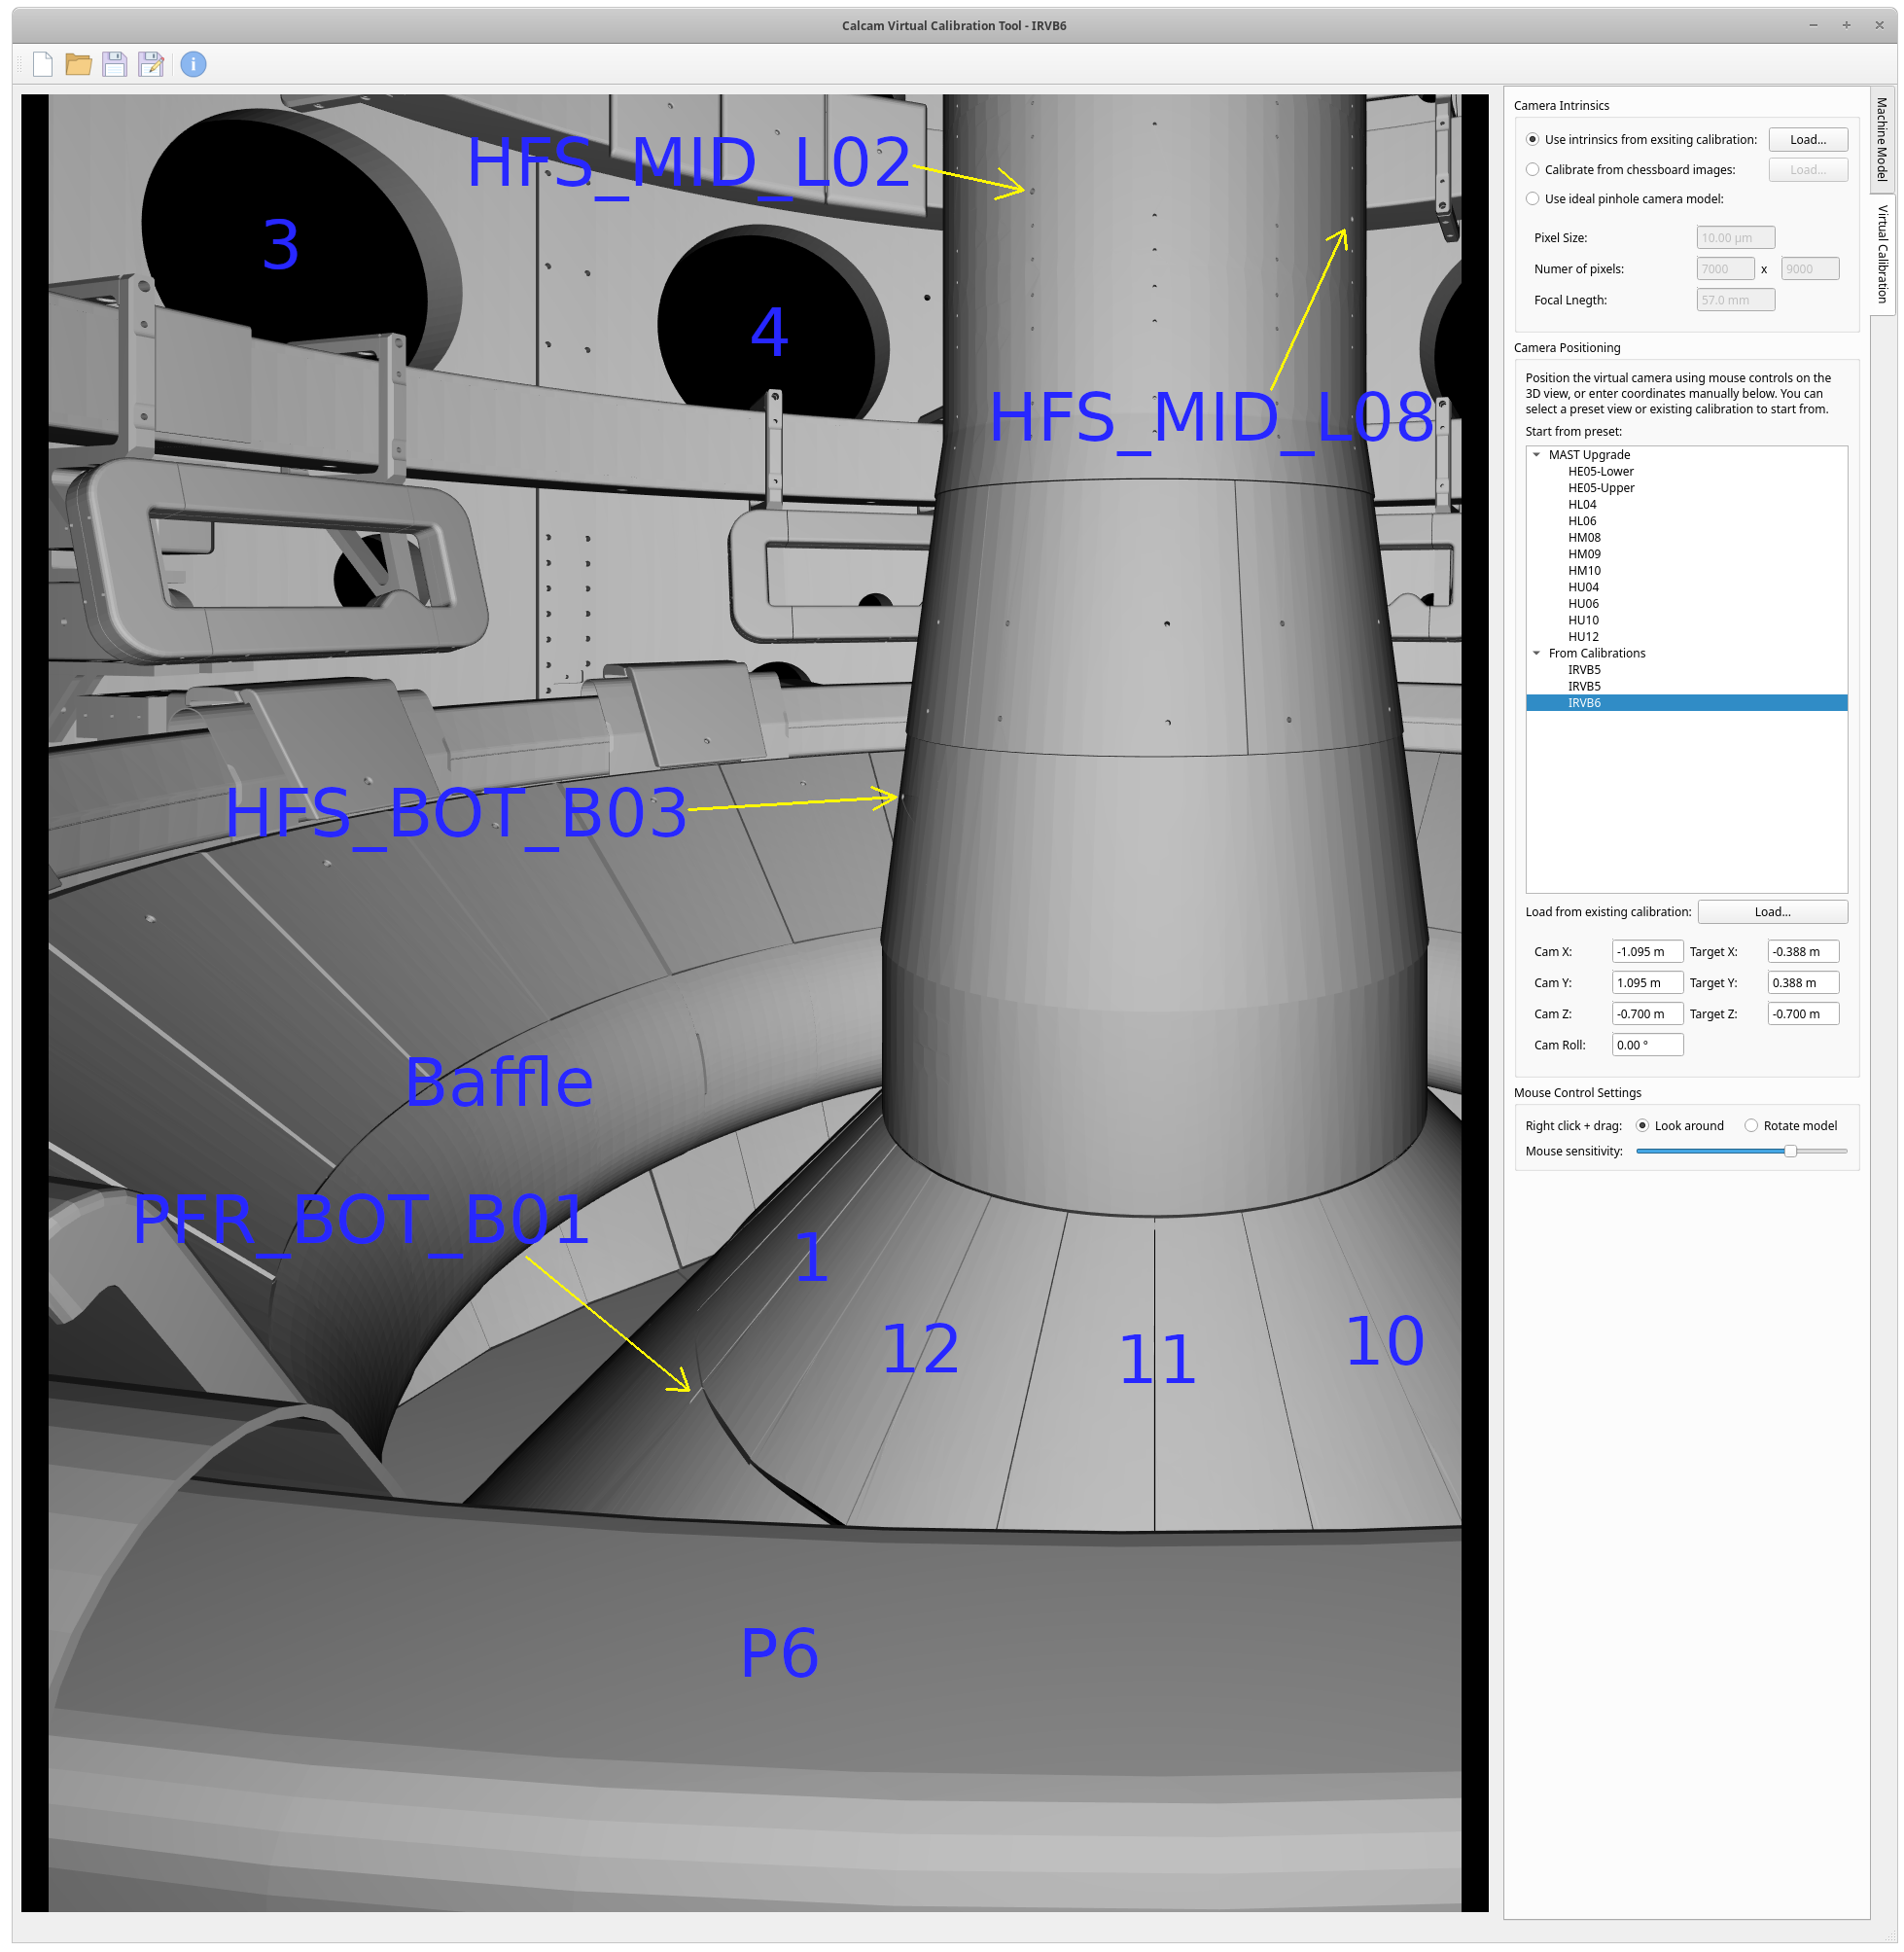
\includegraphics[trim={30 30 450 90},clip,width=0.5\linewidth]{Chapters/chapter2/figs/calcam4.png}
	\caption{Approximate view inside MAST-U as if the IRVB operates as a camera. Blue labelling is used to highlight the various sectors and the fuelling locations in the IRVB field of view (FOV). At the bottom of the image is the coil P6 obstructing the field of view.}
	\label{fig:calcam}
\end{figure}

\begin{figure}[!ht]
     \centering
     \begin{subfigure}{0.48\linewidth}
         \centering
         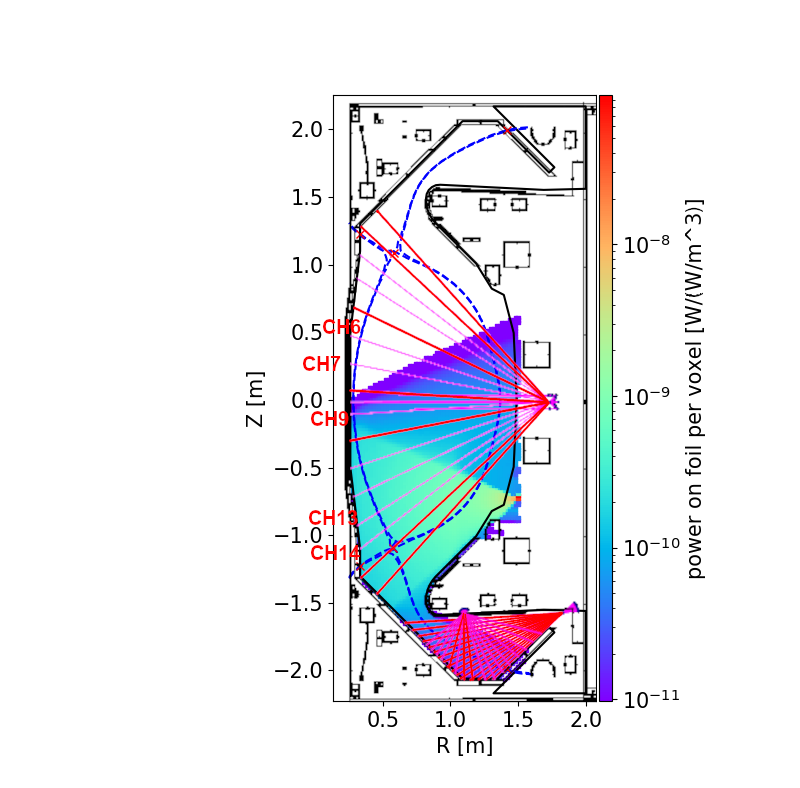
\includegraphics[trim={175 20 65 60},clip,width=\textwidth]{Chapters/chapter2/figs/res_bolo5.png}
         \caption{}
         \label{fig:res_bolo1a}
     \end{subfigure}
     \begin{subfigure}{0.48\linewidth}
         \centering
         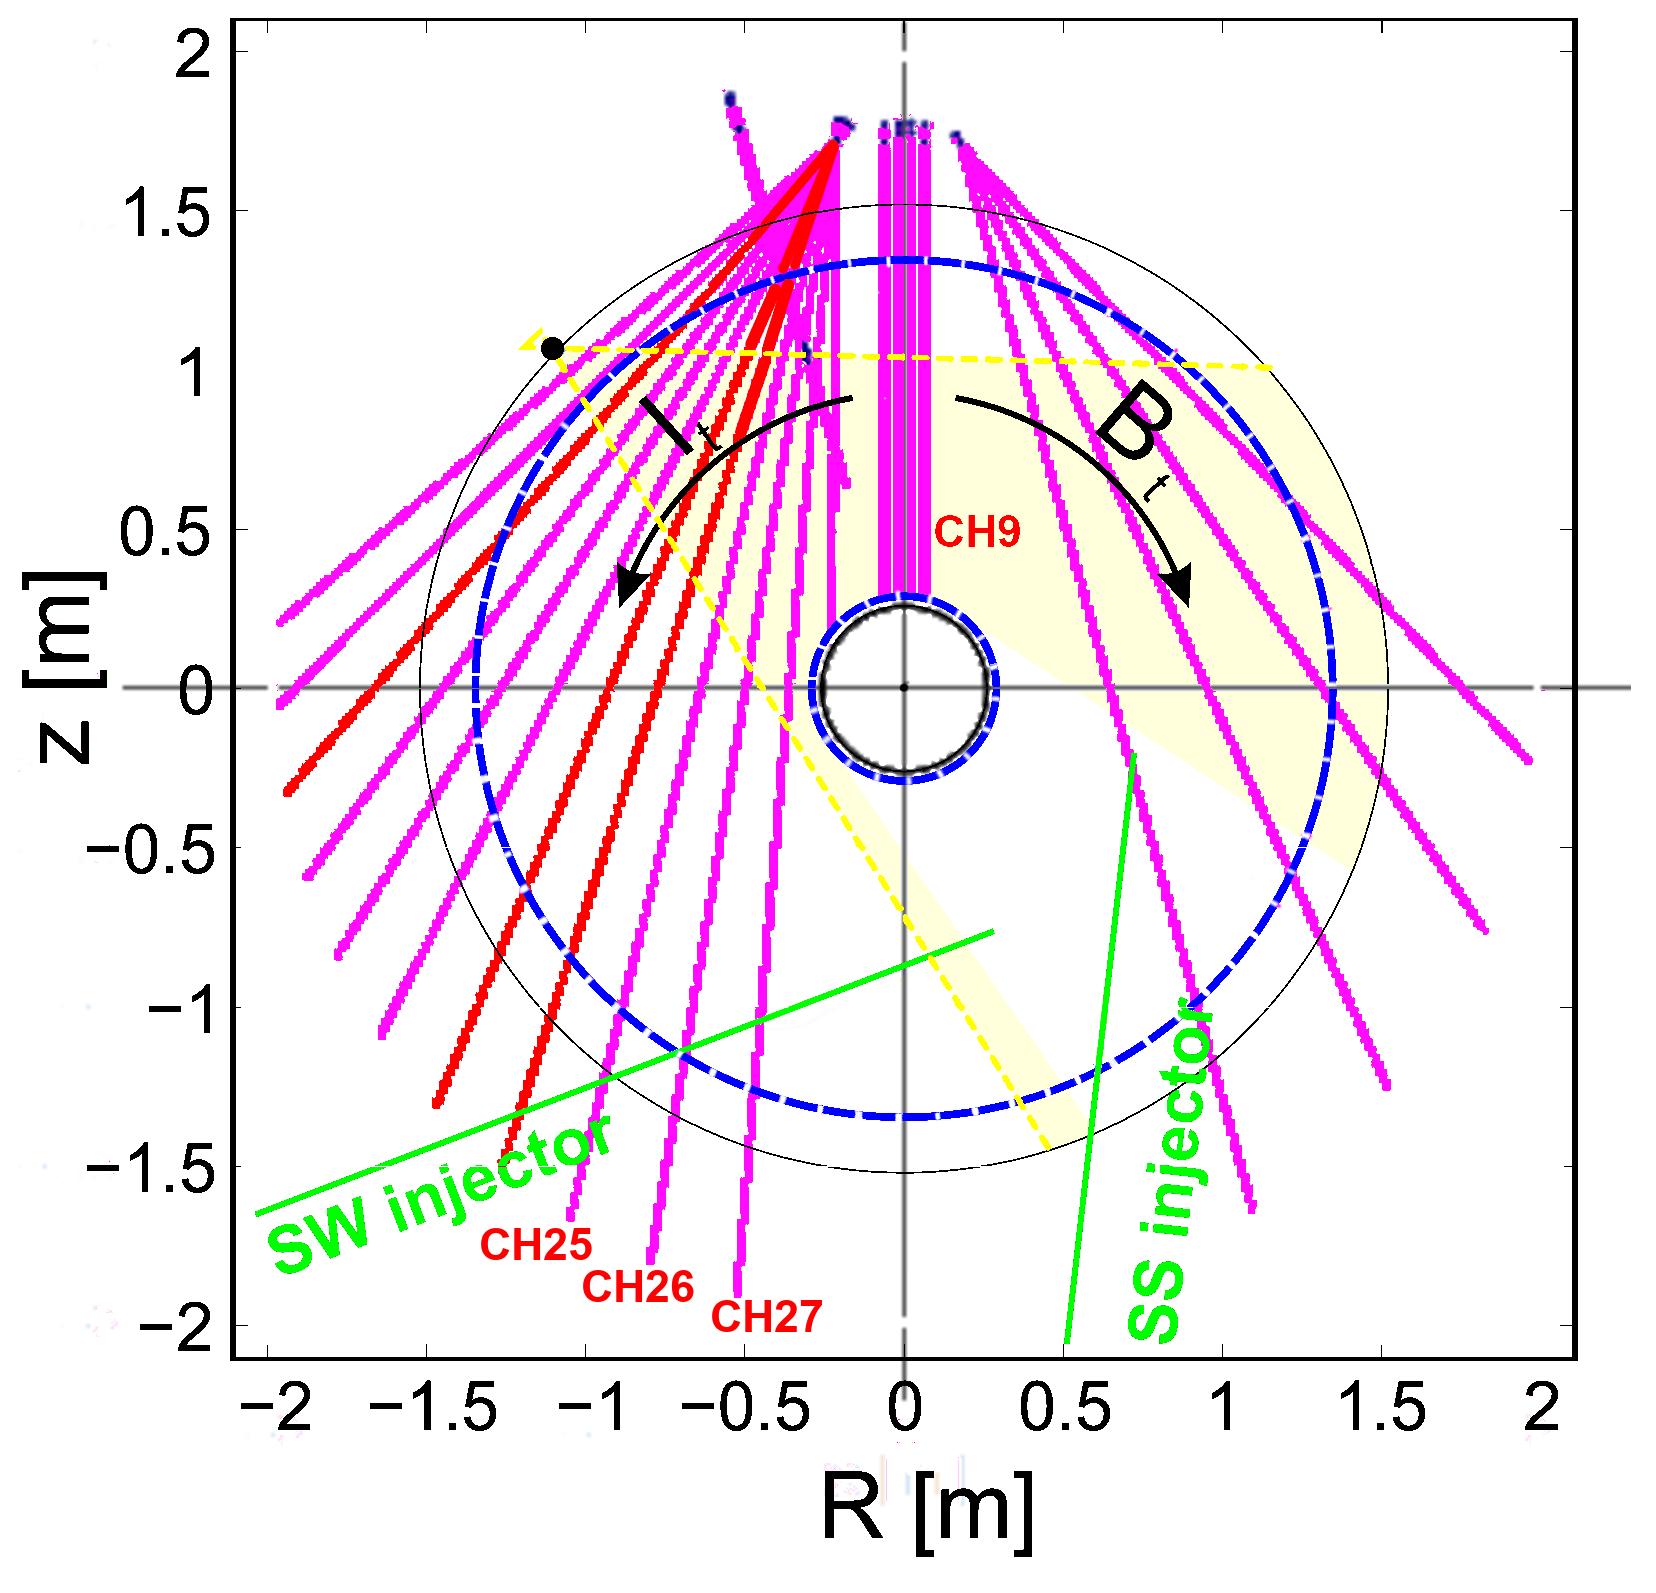
\includegraphics[trim={20 0 70 0},clip,width=\textwidth]{Chapters/chapter2/figs/res_bolo_toroidal3.png}
         \caption{}
         \label{fig:res_bolo1b}
     \end{subfigure}
	\caption{(\subref{fig:res_bolo1a}) Poloidal view of MAST-U showing the comparison of the resistive bolometer system LOS (magenta) with a color plot obtained by scanning all the voxels with a $1W/m^3$ emitter and integrating the power absorbed by the foil, indicating the regions of higher sensitivity of the IRVB. (\subref{fig:res_bolo1b}) Top view of MAST-U showing the position of neutral beam injectors (NBI, green), of the co- and counter-NBI resistive bolometer LOSs and the IRVB FOV (yellow, mostly counter-NBI). Adapted from \cite{Rivero-Rodriguez2018}. For reference the separatrix of a typical plasma is shown as an overlay of a blue dashed line. The resistive bolometer LOSs that will be used in the later analysis are here identified. The LOSs not operational in MU01 are red rather than magenta. The location of CH9 in \subref{fig:res_bolo1b} indicates where the entire core poloidal fan is located.}
    \label{fig:res_bolo1}
\end{figure}


\autoref{fig:res_bolo1} displays the overlap between the coverage and views of the resistive bolometry system and that of the IRVB. The core resistive bolometer LOSs are mostly suited to measure the fairly homogeneous core emissivity profiles on a flux surface, as there is no overlap between the various LOS. The super-x chamber has a good coverage, but only between the  strike point and the entrance to the divertor defined by the baffle. The IRVB is aimed to fill the gap between the two systems. It must be noted that the resistive bolometer sensor is not carbon coated, meaning it has a lower sensitivity to lower energy photons.\cite{VanEden2018} In detached conditions this was assessed to cause a reduction of the brightness of $\sim$15\%.\cite{Sheikh2016}

The assembly holding the foil is composed by a $2.5\mu m$ thick platinum foil from Nilaco, Japan, held between oxygen free copper plates and was originally prepared by NIFS. The foil is the same as that used in Alcator C-mod\cite{Reinke2018a} where it is described in more detail. The foil thickness is optimised to stop photons with energies up to $8.2keV$. \cite{PETERSON2010,Gullikson2022} The foil and its support frame have been spray blackened on both sides with Aerodag® G Graphite Aerosol and calibrated with a procedure analogous to the one described in \cite{Itomi2014}. The layer of graphite helps to absorb radiation in the visible range, avoiding reflection; even if its thickness is larger than the platinum layer\cite{Pandya2014} it should be thermally irrelevant. \cite{VanEden2018} Lower energy photons like visible light represent a minor energy loss channel, but their relevance is expected to increase in deeply detached and cold plasmas, therefore the importance of the coating.\cite{Havlickova2015a} In \cite{Mukai2016} it is shown that this type of coating causes irregularities in the foil, leading to non uniform temperature increases. To alleviate this issue, the carbon layer can be deposited with a vacuum evaporation technique that guarantees reproducibility and uniformity, as done at LHD. \cite{Mukai2016} Given the prototype nature of the present implementation and the availability of a vacuum compatible certified absorber, this spray-blackened foil was deemed sufficient.

\begin{figure}[!ht]
     \centering
     \begin{subfigure}{0.35\linewidth}
         \centering
         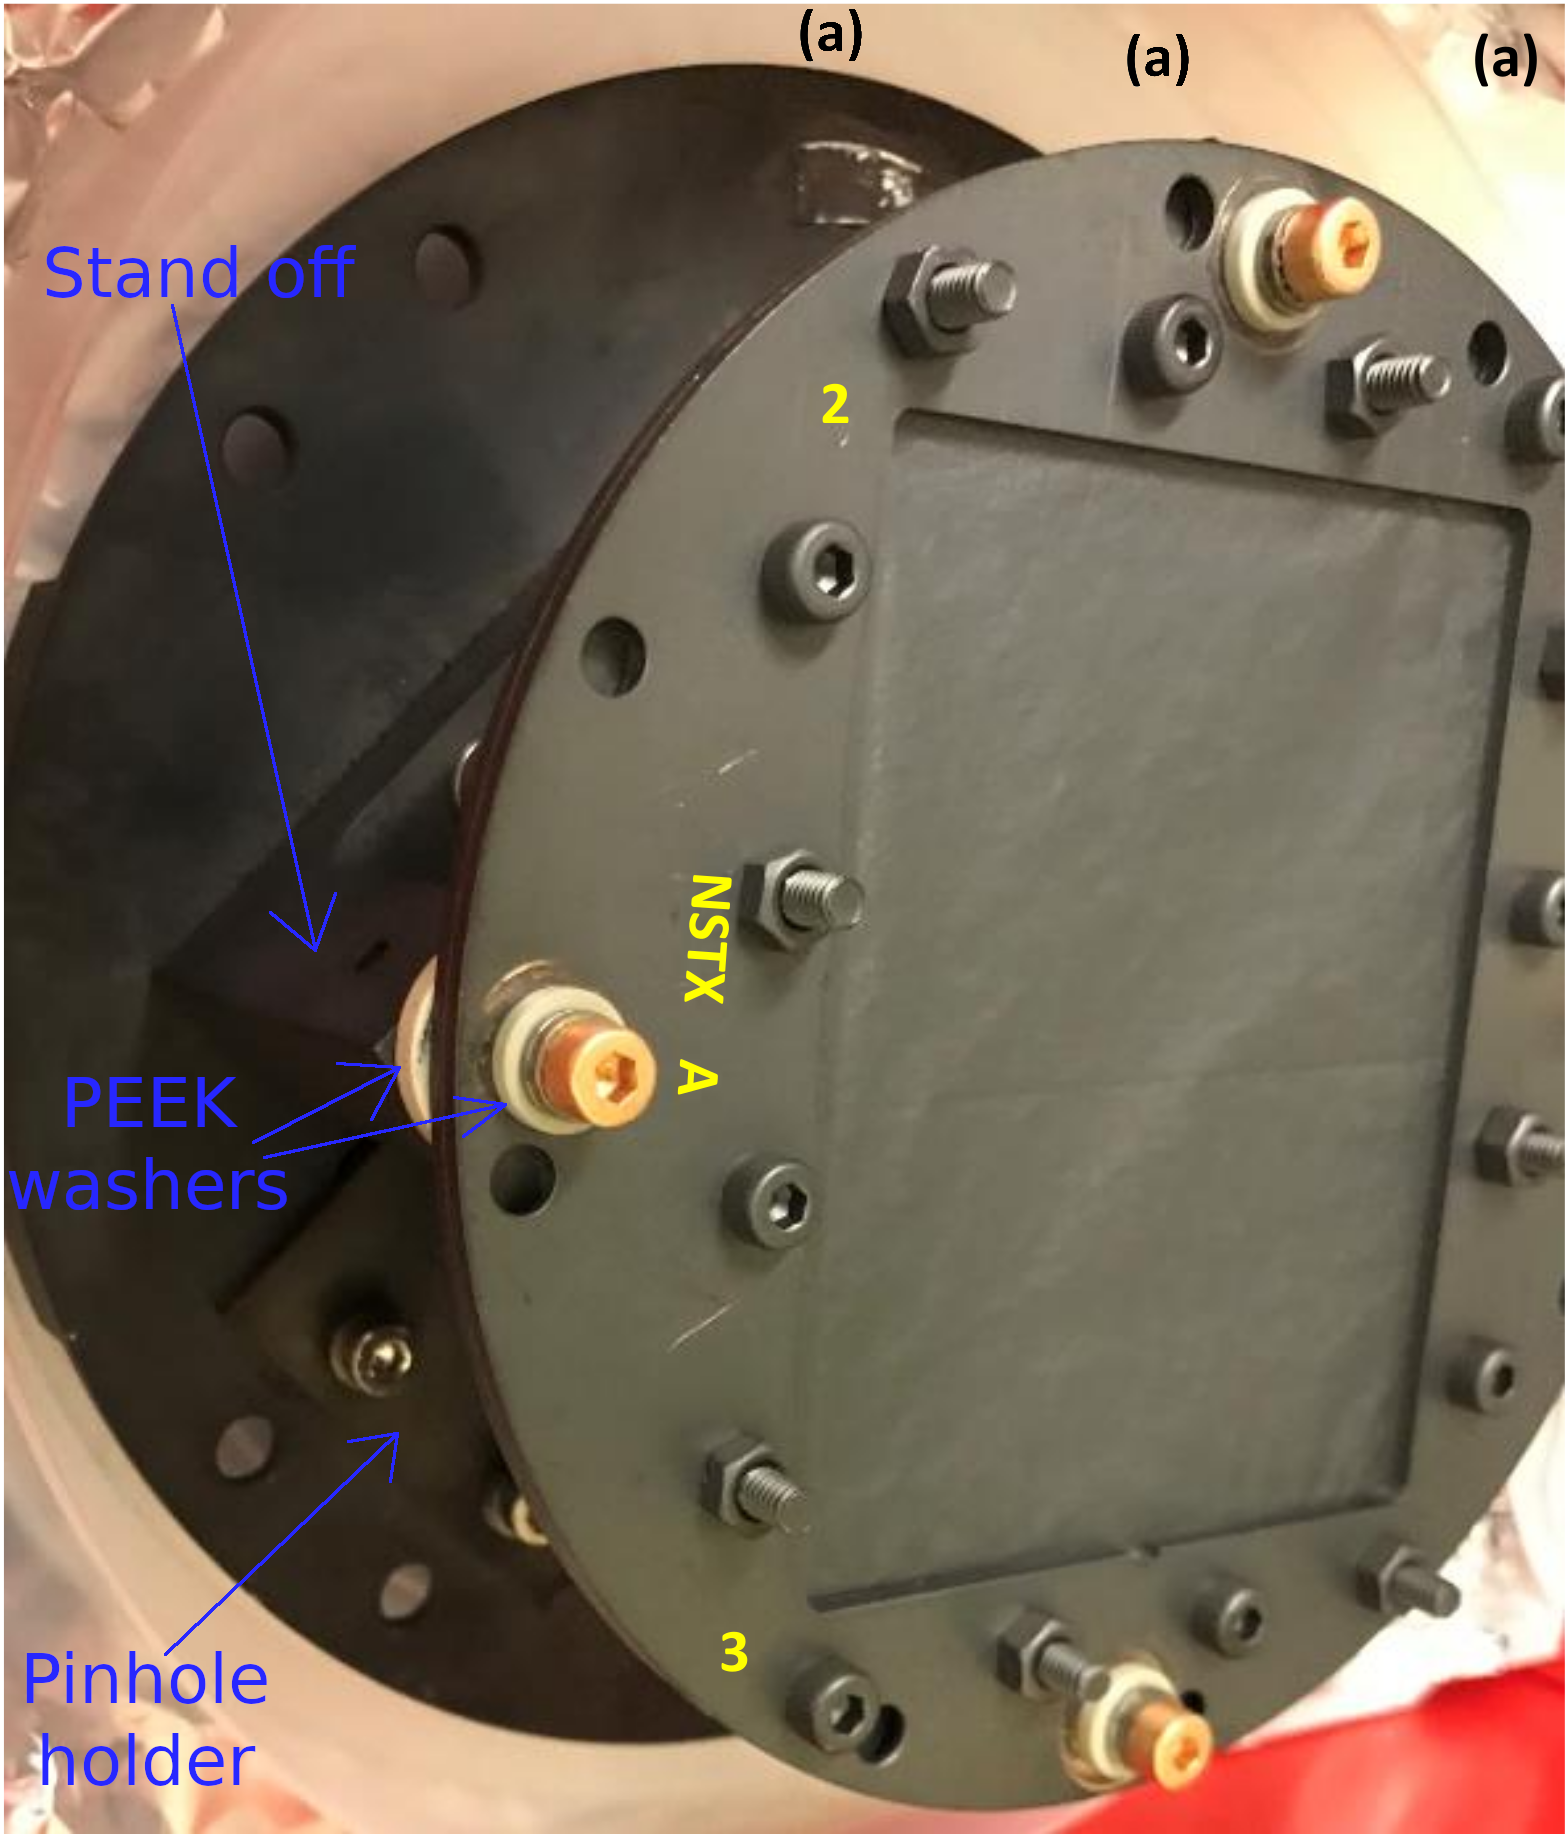
\includegraphics[trim={0 0 600 0},clip,width=\textwidth]{Chapters/chapter2/figs/foil_markings3.png}
        %  \caption{386ms}
         \label{fig:foil markings1}
     \end{subfigure}
     \begin{subfigure}{0.63
     \linewidth}
         \centering
         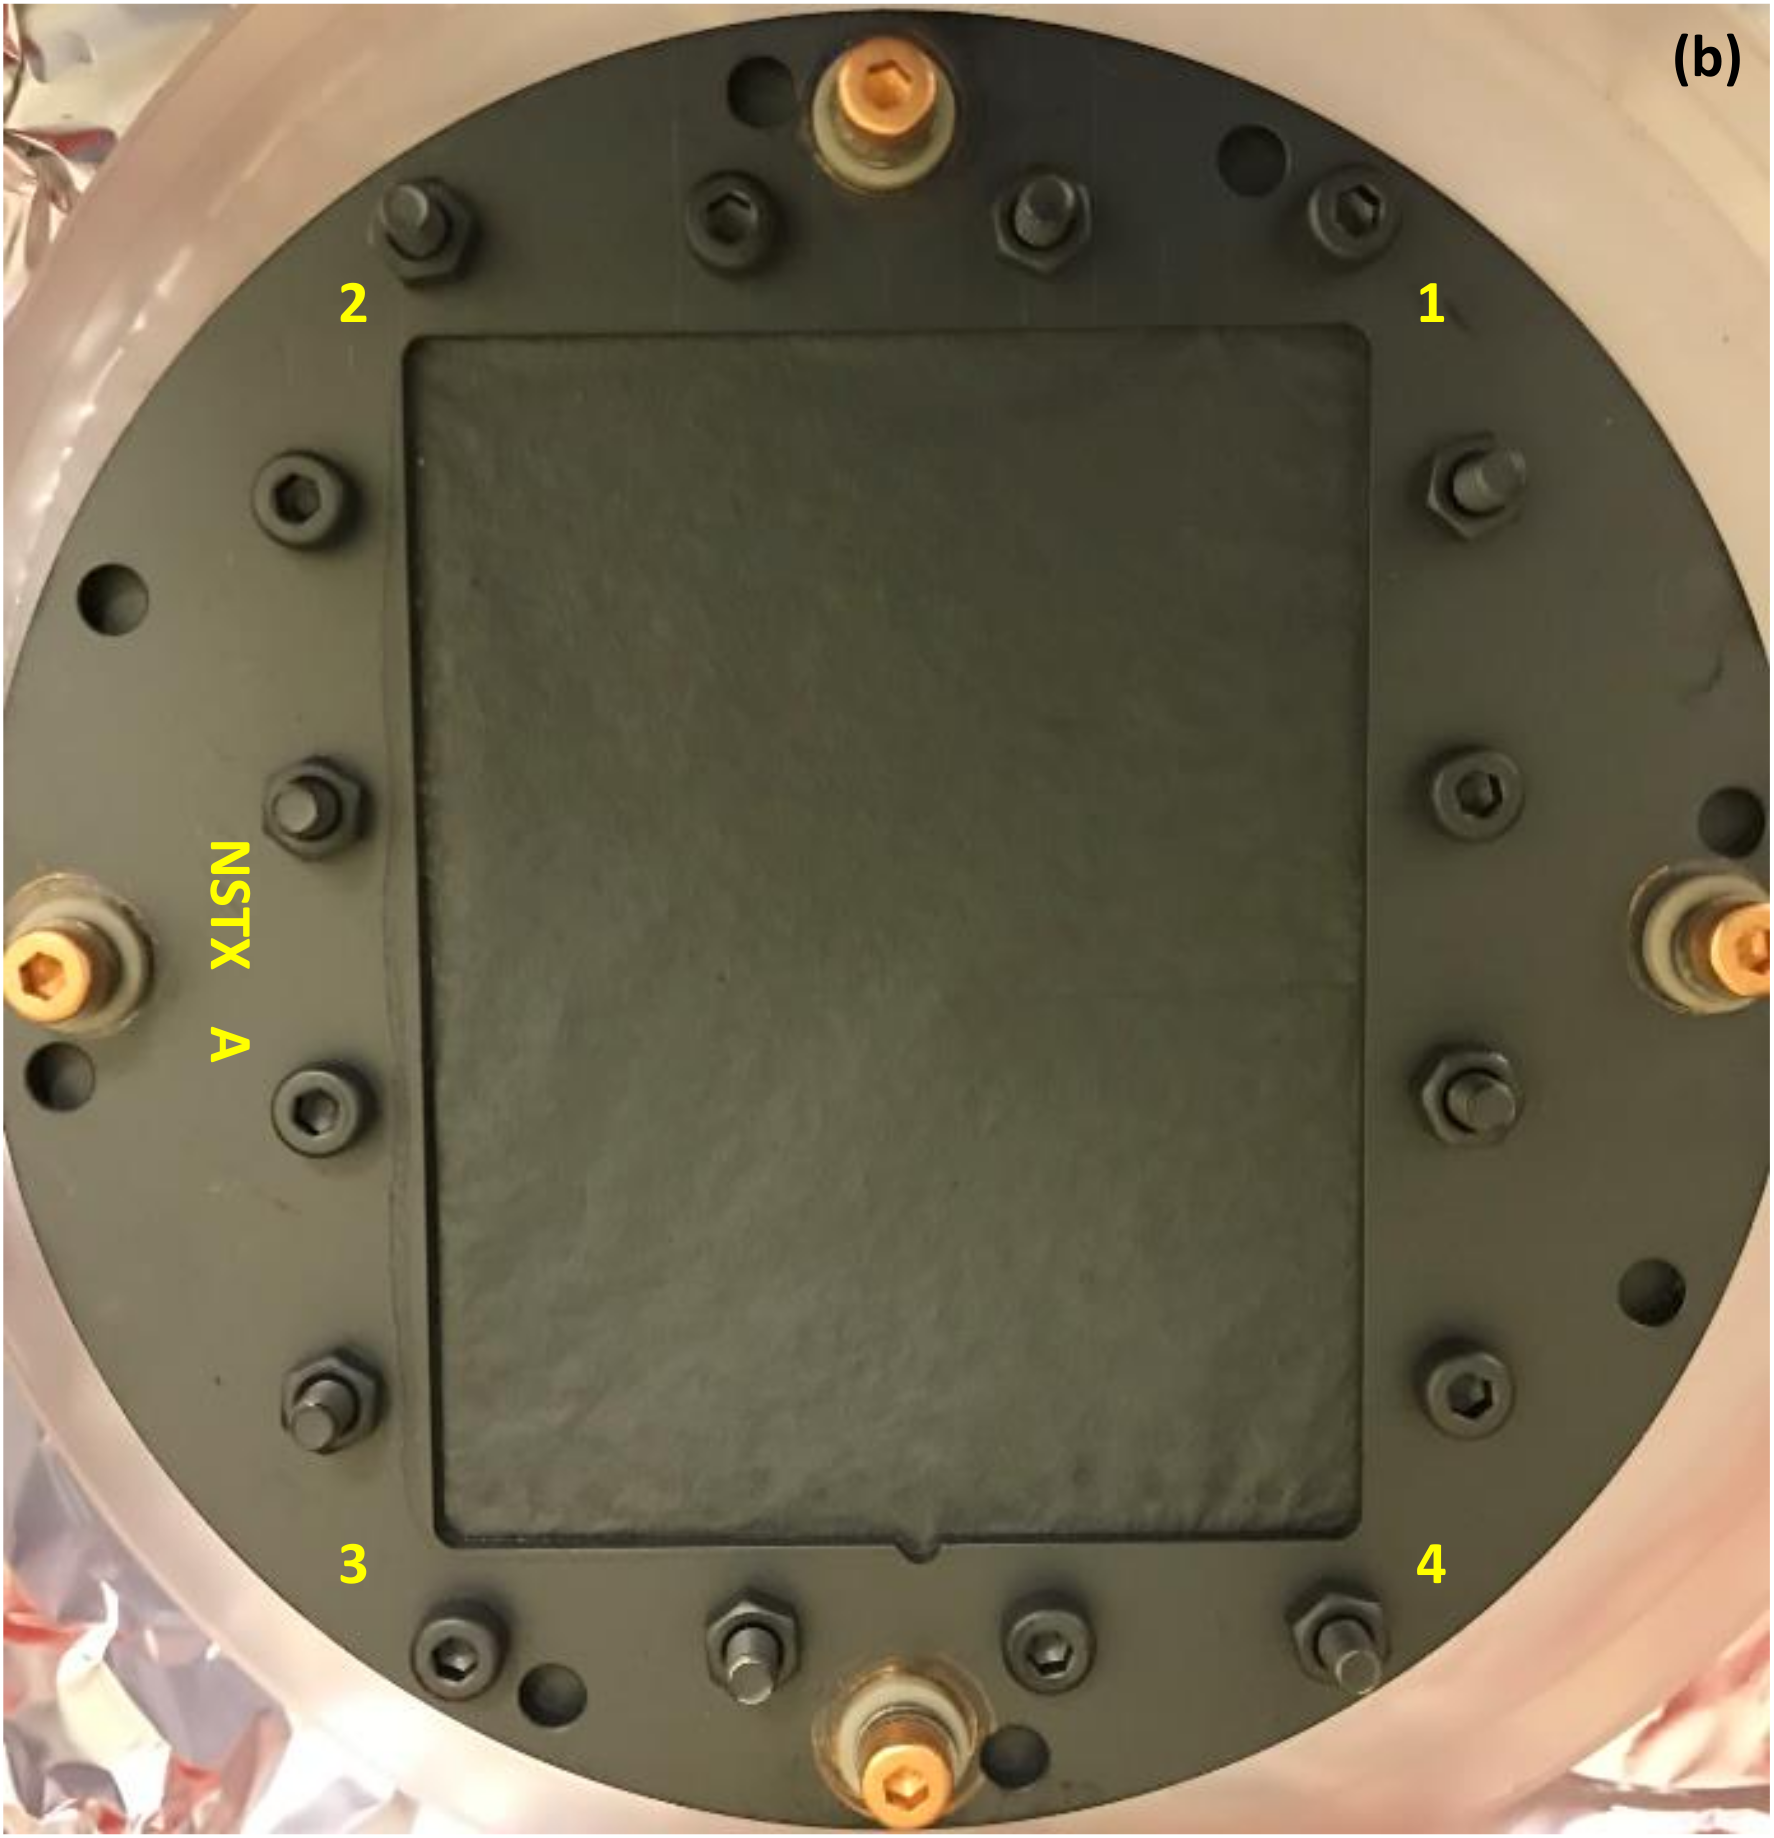
\includegraphics[trim={50 0 0 0},clip,width=\textwidth]{Chapters/chapter2/figs/foil_markings.png}
        %  \caption{511ms}
         \label{fig:foil markings2}
     \end{subfigure}
    \caption{Photographs of the foil in relation of the pinhole (a) and of all the identifying markings (b), taken 23/07/2018.}
    \label{fig:foil markings}
\end{figure}

To guarantee consistency in the positioning and orientation of the foil with respect to the pinhole, a series of markings were inscribed by NIFS on the copper plates as shown in \autoref{fig:foil markings}. The yellow numerical markings are also used to define the thermal calibration supplied with the foil.
The compatibility of the assembly with the thermal expansion caused by the MAST-U VV bake was studied. The bake causes the VV and internal components to reach $\sim110\degree C$ and 120 to $200\degree C$ respectively, likely causing the absorber assembly to reach an intermediate temperature. The thermal expansion coefficients for Cu and Pt are $16 \mu m/mK$ (similar to steel) and $9 \mu m/mK$ respectively. This could have led to stress and thus tearing of the foil, but confidence was gained with the pressure test mentioned in \autoref{MAST-U IRVB design} on the mechanical resilience of the foil. Another item of concern related to the bake is the stability of the carbon coating on the absorber foil. The technical datasheet for Aerodag® G used for coating, indicates that it can be used as lubricant up to $200 \degree C$. Considering the possible failure modes, any piece of carbon detaching from the absorber assembly was expected to stay within the tube, posing no risk for MAST-U operations. The IRVB has ultimately undergone the entire bake cycle prior to MU01 and after inspection did not seem to suffer any damage.

The tube where the foil is installed extends from the vacuum chamber wall to a position close to the plasma, but still safely outside the SOL and potential particle and power loads. The camera images the absorber foil through a $10mm$ thick ZnS view port from Crystran with $4-5 \mu m$ and $8-10 \mu m$ anti reflection coating on both sides and is bolted to the tube. The orientation of the view port with respect to the camera, even if it should not matter substantially, was maintained throughout the test and assembly phases for consistency. The view port assembly was leak checked before final installation with the setup in \autoref{fig:vacuum_setup}. 
The camera, a FLIR SC7500 with InSb detector array, is equipped with a $4-5\mu m$ pass band filter and has a spectral range of $1.5-5.1\mu m$. This model was selected so that the same could be adopted for other diagnostics in MAST-U and the same acquisition software could potentially be developed. This is inconvenient for the IRVB, as the optimal wavelength for a black body radiator around room temperature is around $10-14\mu m$. Considering that the volume between foil and camera is fully enclosed in the IRVB tube and that the temperature of the entire assembly does not deviate appreciably from room temperature during the short duration of the pulse, the use of the filter would not have prevented any stray light to effect the measurements. For this reason the camera was used without the internal filter, increasing the signal. At the maximum frame rate at full frame (383Hz) and 2ms integration time a strong signal around 11000 counts is measured (see \autoref{fig:example_BB_fit}) with saturation at $2^{14}=16384$ counts and a noise floor $\sim5$ counts.
During testing a design flaw of the present IRVB design was discovered. It became clear that, even with the presence of the anti reflection coating, the view port caused the so-called "narcissus effect". This happens when the camera can see its own reflection on the view port, hence "narcissus". The view is orthogonal to the camera FOV, so at its center is the image of the reflection of the sensor array. The detector array is cooled to about $-203\degree C$, while around it the body of the camera is slightly above room temperature. This causes a "dark spot" to appear at the centre of the image. The main difficulty in dealing with the effect arises from the inability to perfectly match the orientation of the view port during calibration and on the machine. Ultimately this systematic error, if stable intra-shot, does not effect the temporal and spatial temperature derivatives on which the analysis primarily relies. In future iterations of the diagnostic, the view port should be angled with respect to the camera so as to reflect light from an area with a more homogeneous temperature and emissivity.

The camera is bolted to aluminum plates cantilevered off an insulating G-10 piece that is connected directly to the vacuum vessel flange (to stop induced current loops) as shown in \autoref{fig:IRVB_components}. The aluminum plates holding the camera have multiple holes so that the camera can be located at 4 fixed distances from the the view port (8.7, 11.2, 13.7, $16.2cm$), with the closest being the one with the foil in focus. The ability to vary the camera location allowed us to progressively test the compatibility of the camera with magnetic field. That data was collected during the commissioning phase of the MAST-U magnets while the camera was first as far as possible from the VV. Once the maximum field was reached the camera was then progressively moved towards its final position whilst checking that no anomalies in its operation arose. The camera operated normally at all distances, making a magnetic shield around it unnecessary.

The IRVB tube was installed on MAST-U in November 2018 while all parts outside the vacuum vessel by early 2021. The calibration of the system was performed in 2018.


\section{System calibration}\label{System calibration}
Before scientific utilization, the IRVB diagnostic has to be properly calibrated. This includes the temperature response of the IR camera, the thermal response of the foil and spatial alignment of the pinhole and camera. Laboratory tests can be performed for the first two calibrations, while the third was verified during operation, using observed features inside the tokamak.

% old sections where the method uses the black body source as close as possible to the window
% \subsection{Counts to temperature model}\label{Counts to temperature model}
% The temperature calibration is the procedure used to convert the camera row data from counts to temperature. It involves defining the mathematical model for the conversion and finding the coefficients required. Once defined it can be applied to MAST-U data to obtain the IRVB foil temperature.
% The surface of the foil is approximated as a black body emitter. The photons emitted by a BB source within the camera integration time can be modelled as \autoref{eq:BBphotons1}


% \begin{equation}
% {\Phi}_p (T) = \epsilon i \int_{ {\lambda}_1 }^{ {\lambda}_2 } {\frac{2 \pi c } { {\lambda}^4 } \frac {1} { e^{\frac {hc} {\lambda k T}} -1} {d \lambda} }
% \label{eq:BBphotons1}
% \end{equation}

% with $\epsilon$ emissivity, $i$ integration time, $\lambda$ wavelength and $\lambda_1-\lambda_2$ the range allowed by the camera filter and $T$ the surface temperature.
% To simplify the calculations an interpolator is built such that

% \begin{equation}
% \frac {{\Phi}_p (T)} {T} = \alpha (T) , T = {\alpha}_r ({\Phi}_p)
% \label{eq:BBphotons2}
% \end{equation}

% The number of photons reaching the camera are going to be proportional to the number of emitted photon ($a_1$), with an additional offset due to thermal photons originated from other solid surfaces and the air ($a_2$). This offset will be approximately constant because it will not depend on the surface temperature observed by the camera.
% The presence of the view port between camera and the source of BB radiation will decrease the number of thermal photons reaching the camera ($a_3$) and potentially modifies the constant offset ($a_4$).
% Assuming that the number of counts is proportional to the number of photons, and that this does not depends on the photon wavelength, the number of camera counts can be expressed as:

% \begin{equation}
% C = a_1 \cdot a_3 \cdot {\Phi}_p (T) + a_2 + a_4
% \label{eq:BBphotons3}
% \end{equation}

% with $a_1\in[0,\infty]$ and $a_2\in[-\infty,\infty]$ the proportional and constant component for the counts without the view port and $a_3\in[0,1]$ and $a_4\in[-\infty,\infty]$ the modifiers for the view port case. $T_0$ and $C_0$ are the temperature and counts relative to the initial conditions at the beginning of the shot (room temperature).
% In order to calculate all 4 coefficients 2 temperature ramps are required, one with and one without view port. When changing the temperature of the BB source the camera counts have to be monitored to make sure to collect the data only after they have stabilised.
% The counts/temperature curves obtained are then fit to return the coefficients. The power absorbed by the IRVB foil is obtained using the temperature increase over the profile before the pulse ($T_0$ and $C_0$), so the constant offset from the calibration will not impact the results while its uncertainty will impart the result uncertainty, even if usually negligibly.
% Once $a_1 \cdot a_3$ is determined the temperature is calculated as:

% \begin{equation}
% T = {\alpha}_r ( {\Phi}_p(T)) = {\alpha}_r \left (\frac {C - a_2 - a_4} {a_1 \cdot a_3} \right ) = {\alpha}_r \left (\frac {C - C_0} {a_1 \cdot a_3} + {\Phi}_p (T_0) \right )
% \label{eq:BBphotons4}
% \end{equation}


% \subsection{Temperature calibration}


% In order to test every pixel of the camera with the limited size of the BB source available the source was taken as close as possible to the view port making it out of focus. This could be done as the whole surface of the BB cavity emits the same amount of radiation isotropically. For the pixels whose entire field of view is inside the source from when it is in focus to when it's closer the etendue is conserved, allowing to perform the calibration. A series of measurements was performed to verify this by changing the distance between the camera and the black body source at room temperature and with a hot black body source. The black body source employed was a MIKRON M315HT with a range of ambient temperature $+10\degree C/+450\degree C$ therefore to calibrate the camera in the useful temperature of ambient $+0\degree C/+10\degree C$ the ambient temperature was lowered to about $5\degree C$. The infrared camera is equipped with 2 distinct digitizers therefore the calibration will be operated independently for each. This means that formally the two digitizers behave as 2 distinct instruments; the power absorbed by the foil will be calculated independently for each and then averaged, causing a reduction of the maximum frame rate from 383Hz to 192Hz.

% \hl{example of vignetting and narcissus}

% \begin{figure}[!ht]
% 	\centering
% 	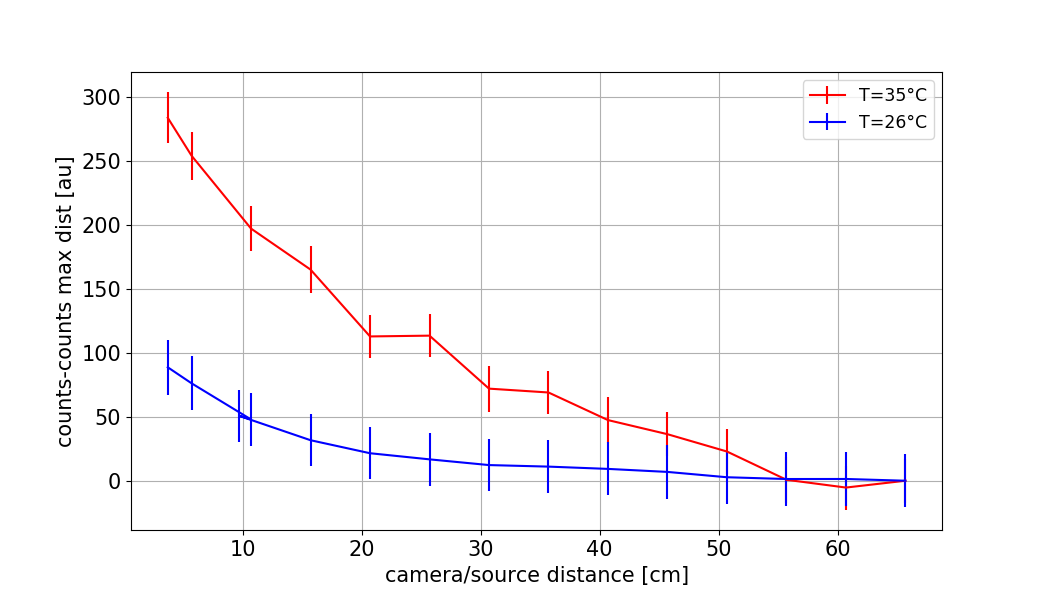
\includegraphics[trim={40 5 70 50},clip,width=\linewidth]{Chapters/chapter2/figs/counts vs distance2.png}
% 	\caption{Average counts for pixels that always image the inside of the black body source. The viewport was not present for this measurements. The error bar represent the variation of the reading within the region.}
% 	\label{fig:counts vs distance2}
% \end{figure}
% In \autoref{fig:counts vs distance2} is shown the variation with distance of the average counts for pixels that always image the black body source. The variation is small but not negligible (400 counts correspond to about $1\degree C$ variation). The cause of the variation cannot be identified but could be reflections or the effect of line absorption in the observed wavelength window ($2.5-5 \mu m$, $CO_2$ has a line at $\sim 4.2 \mu m$). The configuration that is closer to the experimental conditions is the one with the black body source as close as possible to the view port as vacuum is present inside the vessel so this will be used.

% \begin{figure*}
% 	\centering
% 	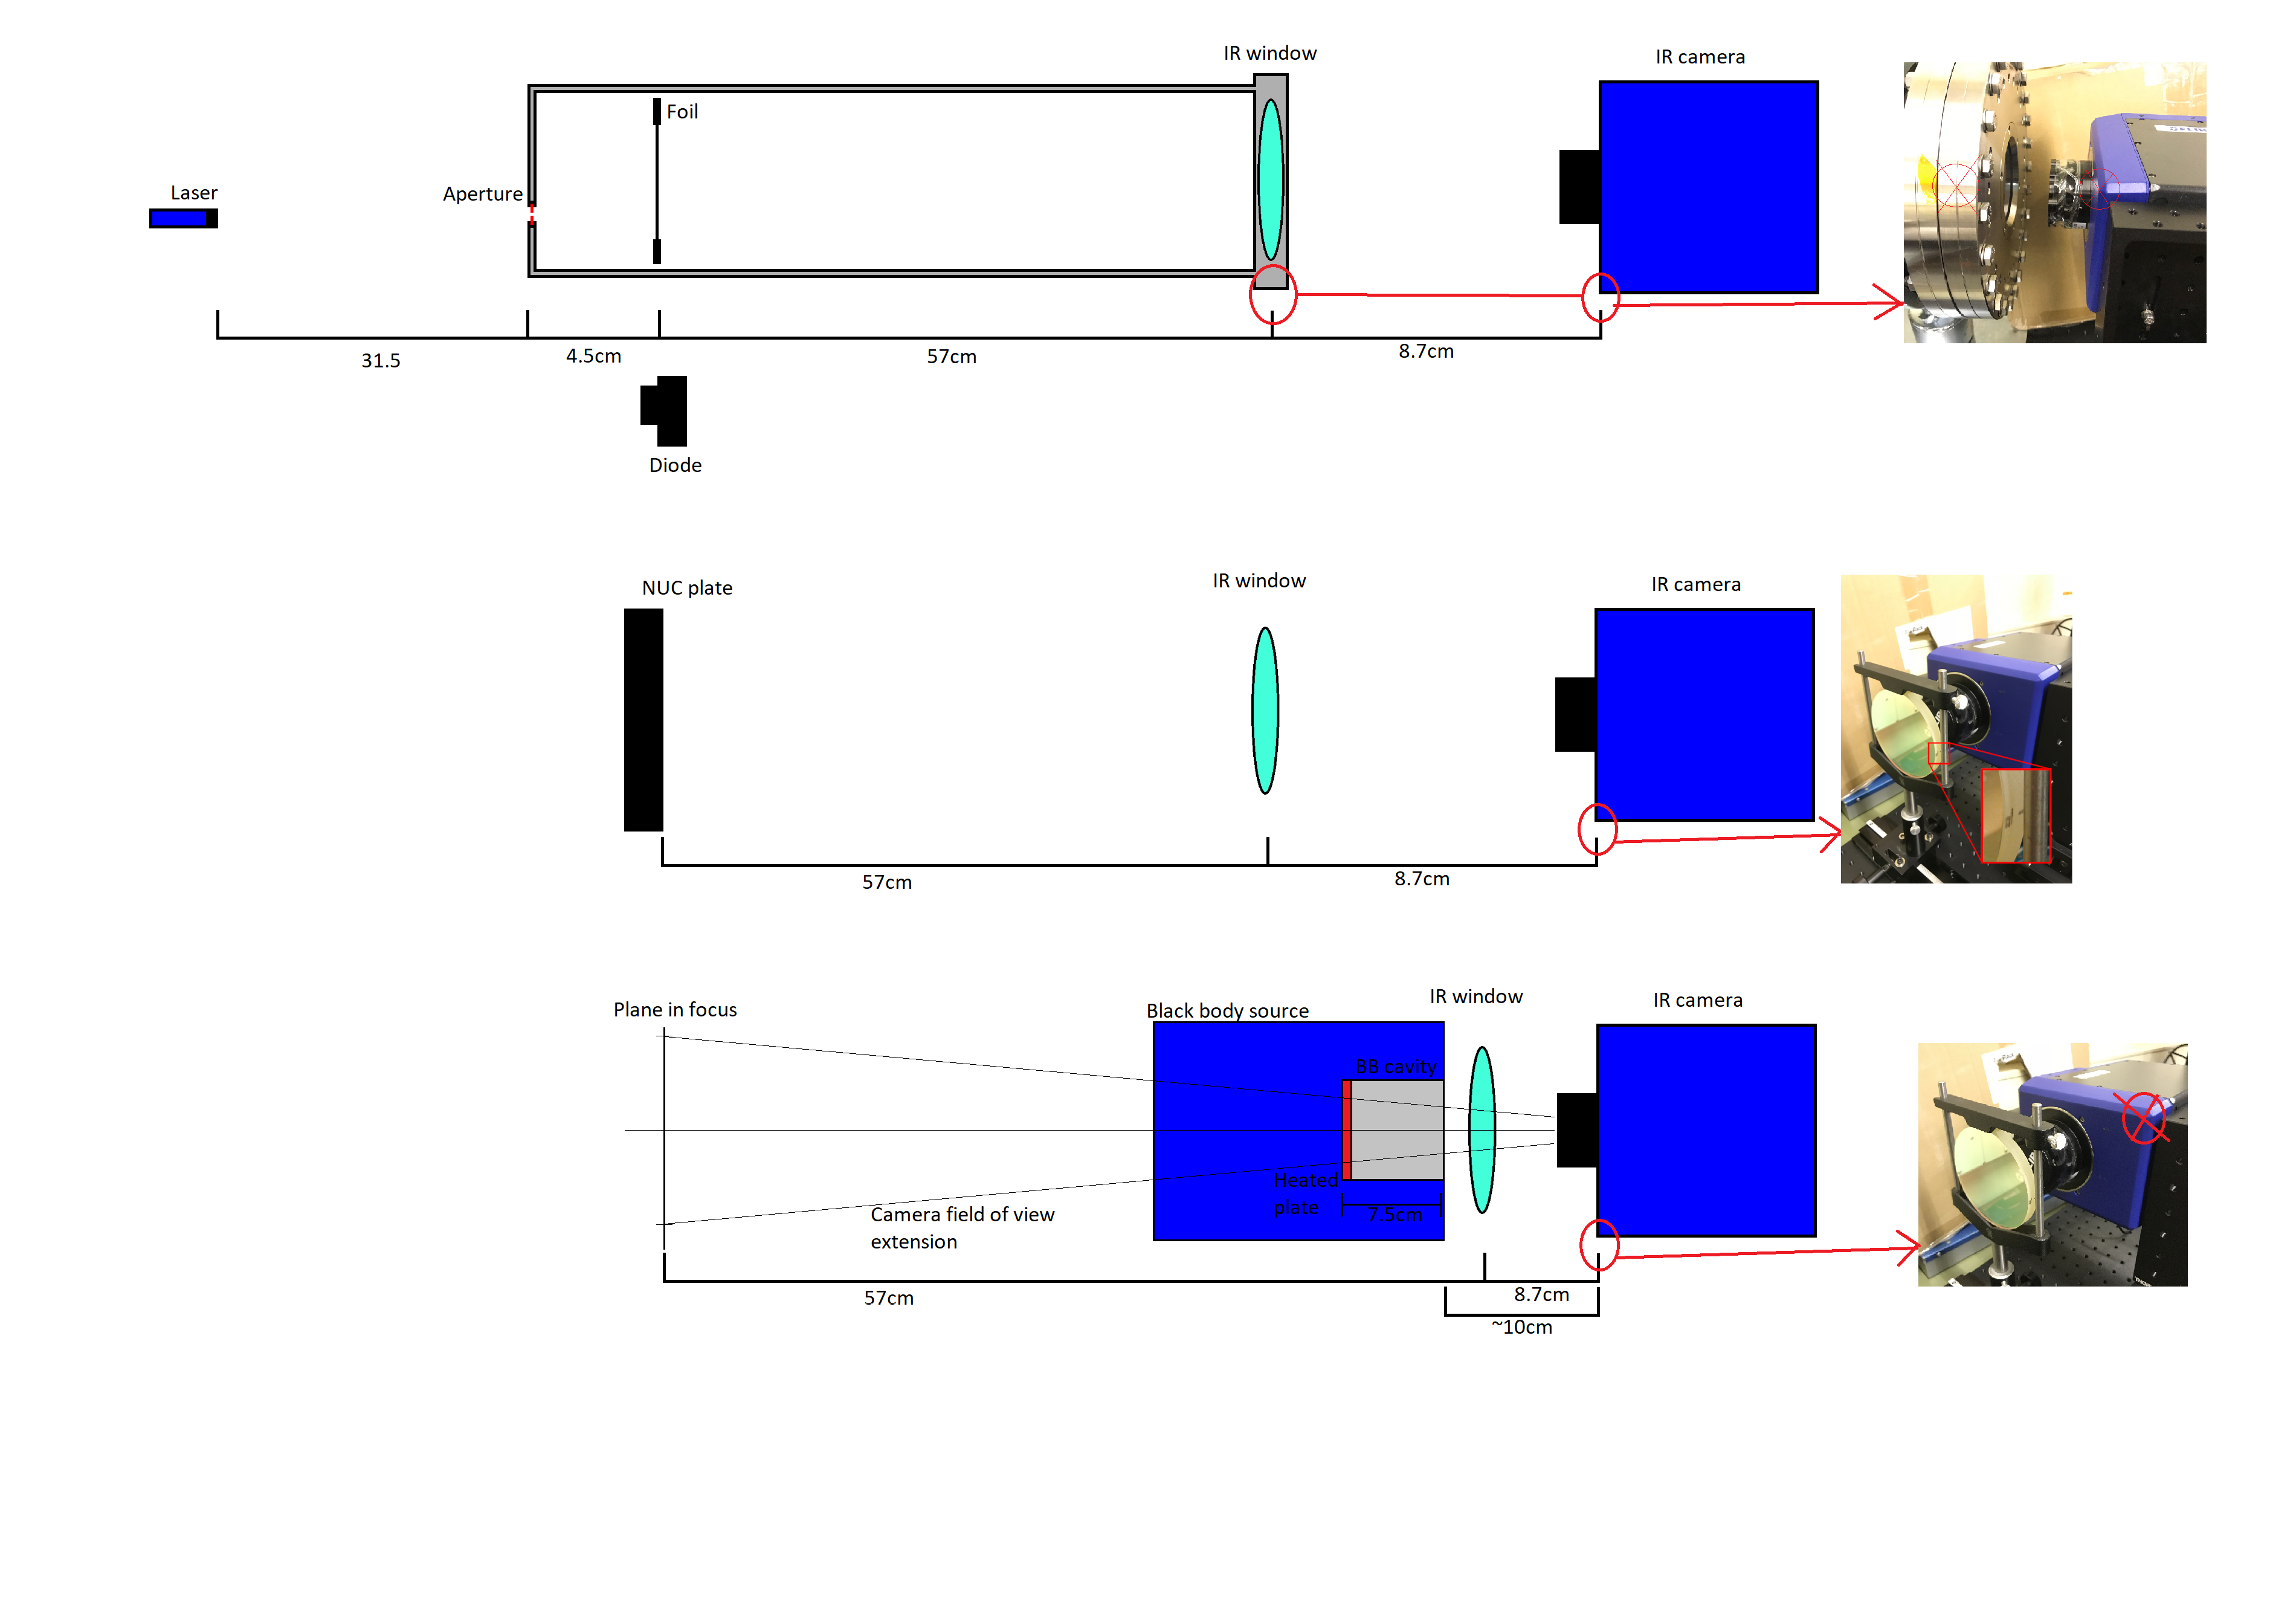
\includegraphics[trim={750 300 0 1200},clip,width=\linewidth]{Chapters/chapter2/figs/calib_schematics.png}
% 	\caption{Schematic of the calibration setup. The plane in focus correspond to the distance at which the IRVB foil is. The view port is at the same distance from the camera as when installed on MAST-U. The location used to measure the distance of the camera from other objects is marked in red.}
% 	\label{fig:BBcalib}
% \end{figure*}

% The geometry of the calibration is represented in \autoref{fig:BBcalib}. As it takes time for the black body source temperature to stabilise the view port is installed in such a way that it can reliably removed and placed back with the same orientation. This allows to do both temperature scans with and without view port in a single source temperature scan.

% \begin{figure}[!ht]
%      \centering
%      \begin{subfigure}{\linewidth}
%          \centering
%          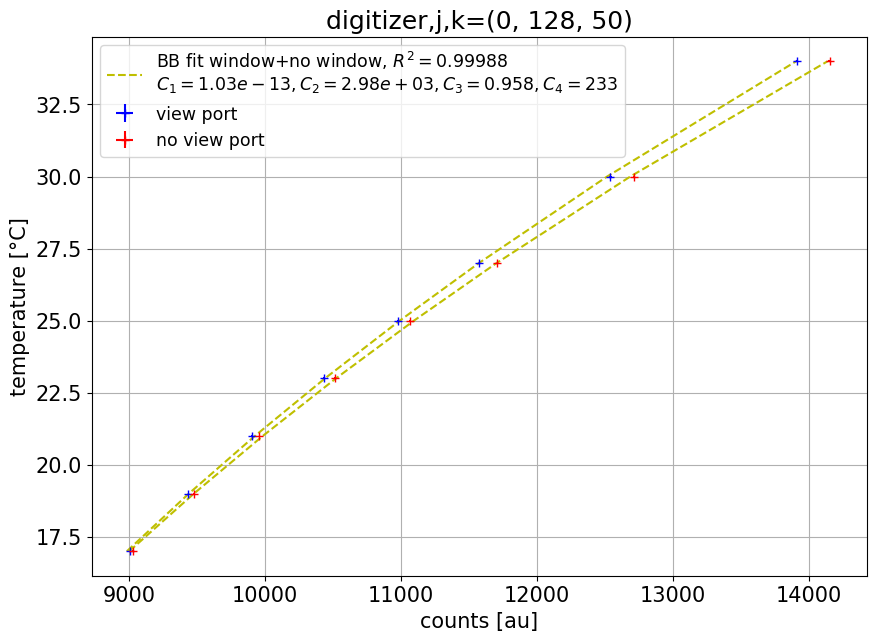
\includegraphics[trim={0 0 0 25},clip,width=\linewidth]{Chapters/chapter2/figs/example_BB_fit(0, 128, 50).png}
%          \caption{digitizer 0, pixel (128,50)}
%          \label{fig:example_BB_fit(0, 128, 50)}
%      \end{subfigure}
%      \hfill
%      \begin{subfigure}{\linewidth}
%          \centering
%          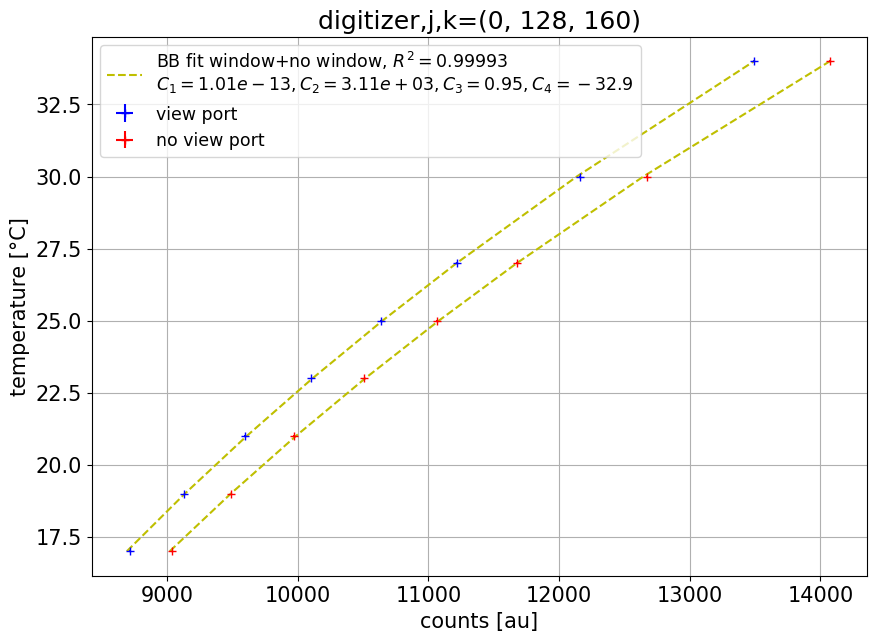
\includegraphics[trim={0 0 0 25},clip,width=\linewidth]{Chapters/chapter2/figs/example_BB_fit(0, 128, 160).png}
%          \caption{digitizer 0, pixel (128,160)}
%          \label{fig:example_BB_fit(0, 128, 160)}
%      \end{subfigure}

%     \caption{Comparison of the temperature calibration curves for a pixel at the centre of the aberration (\subref{fig:example_BB_fit(0, 128, 160)}) with one on its side (\subref{fig:example_BB_fit(0, 128, 50)}). In yellow is indicated the fit of the data with \autoref{eq:BBphotons3} and in the legend the corresponding coefficients.}
%     \label{fig:example_BB_fit}
% \end{figure}

% The result of the scan for two pixels, one at the centre of the aberration caused by the view port and one on its side, are shown in \autoref{fig:example_BB_fit}. \autoref{eq:BBphotons3} can reproduce the measurements with high accuracy and the effect of the presence of the view port can be readily extracted. As expected, most of the flat offset is in $a_2$ while only a minor component in $a_4$.

% The results of the calibration for the entire foil are shown in \autoref{fig:BBcaliba1}, \ref{fig:BBcaliba3} and \ref{fig:BBcaliba1a3SNR}. The $a_1$ coefficient seems completely not effected by the narcissus effect. Conversely the corrective factor $a_3$ seems dominated by it, while still being $>0.95$ across the thole field of view with a relative variation less then half of $a_1$. The $a_2$ and $a_4$ coefficients are irrelevant as are not used in the temperature and power calculations.

% \begin{figure}[!ht]
% 	\centering
% 	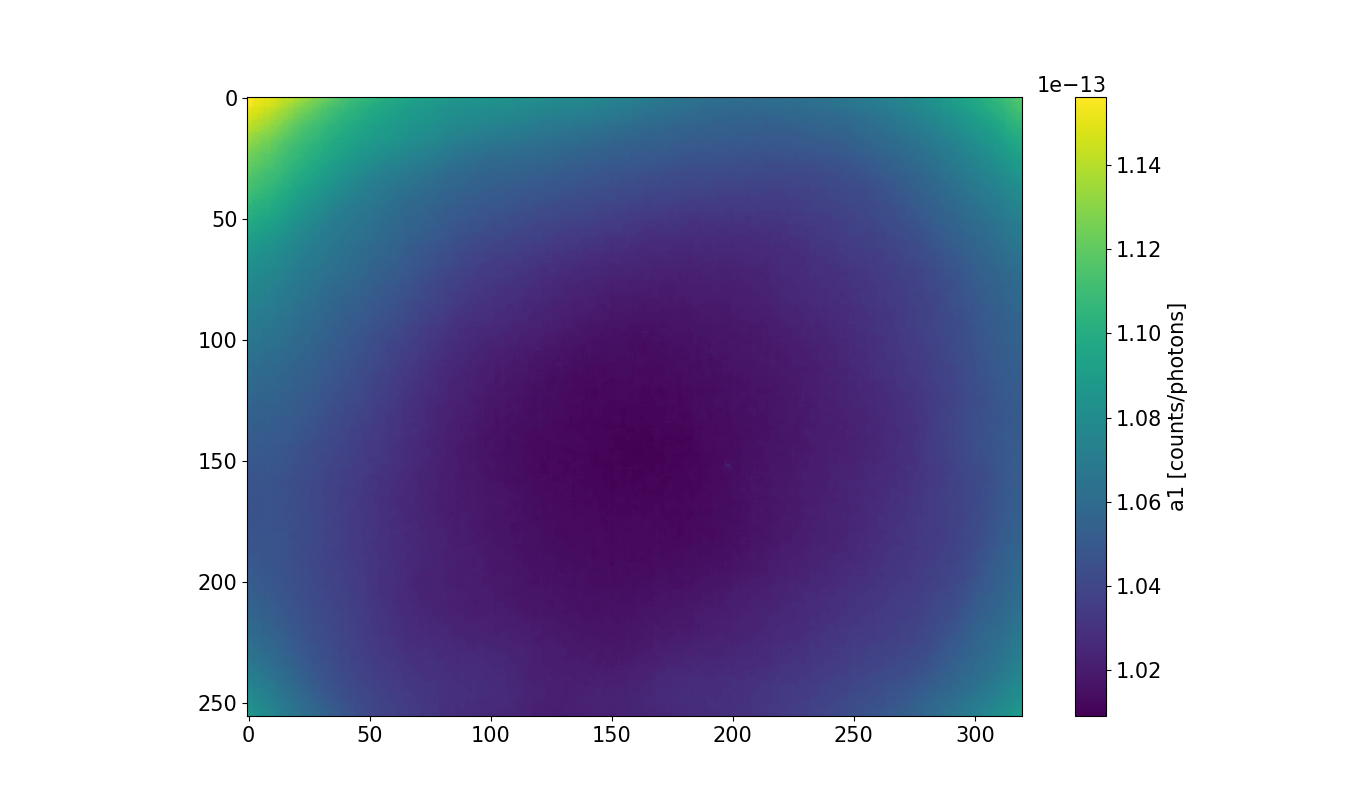
\includegraphics[trim={140 40 120 50},clip,width=\linewidth]{Chapters/chapter2/figs/calib_a1_2.png}
% 	\caption{$a_1$ coefficient obtained via calibration with BB source}
% 	\label{fig:BBcaliba1}
% \end{figure}
% \begin{figure}[!ht]
% 	\centering
% 	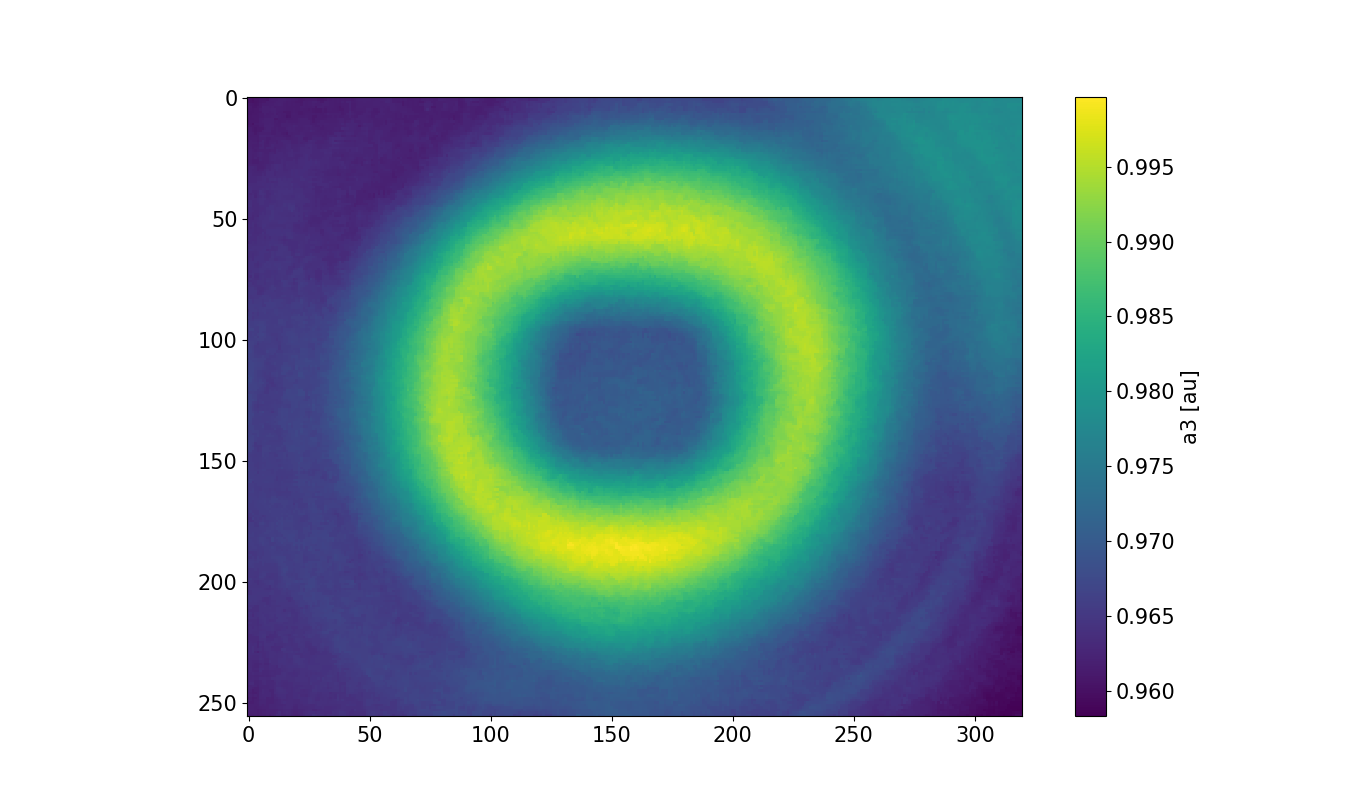
\includegraphics[trim={140 40 120 50},clip,width=\linewidth]{Chapters/chapter2/figs/calib_a3_2.png}
% 	\caption{$a_3$ coefficient obtained via calibration with BB source}
% 	\label{fig:BBcaliba3}
% \end{figure}
% \begin{figure}[!ht]
% 	\centering
% 	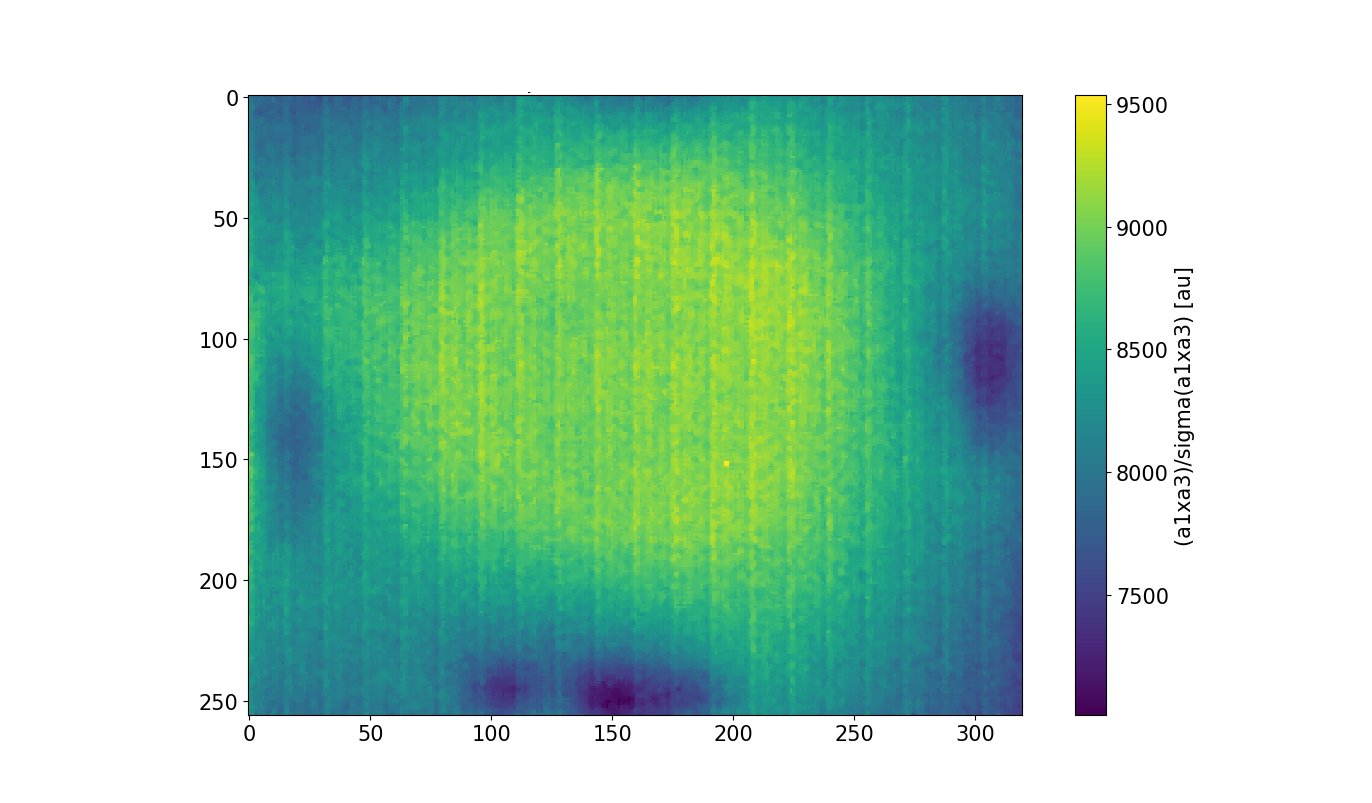
\includegraphics[trim={140 40 120 50},clip,width=\linewidth]{Chapters/chapter2/figs/calib_a1a3SNR_2.png}
% 	\caption{$a_1 a_3 / \sigma_{a_1 a_3}$ obtained via calibration with BB source}
% 	\label{fig:BBcaliba1a3SNR}
% \end{figure}

% To further verify the effect of the distance 3 separate calibrations were performed: camera and BB source as close as possible ($\sim 10cm$, some room was necessary for the view port in between the two), as far as possible (with the whole field of view still inside the source, $\sim 18cm$) and with the source in focus ($65.7cm$).

% \begin{figure}[!ht]
% 	\centering
% 	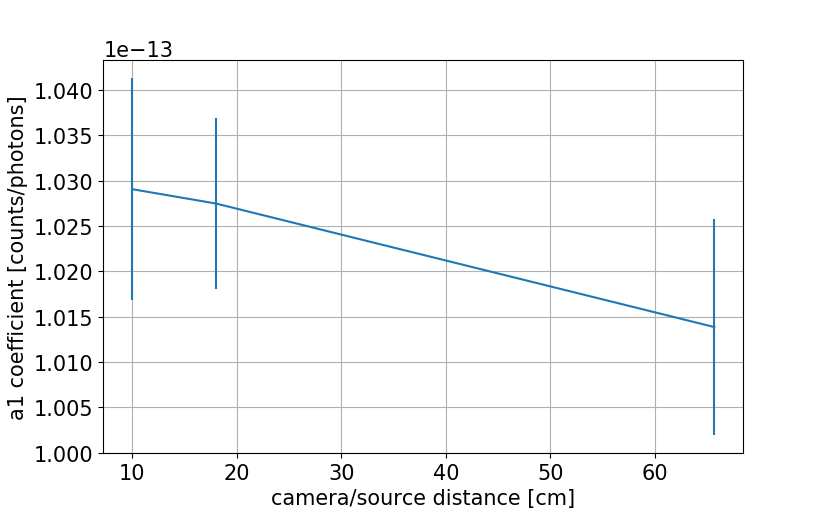
\includegraphics[trim={0 0 40 30},clip,width=\linewidth]{Chapters/chapter2/figs/a1 vs distance.png}
% 	\caption{Variation with the source to camera distance of the average of the a1 coefficient over pixels that image the inside of the black body source. The viewport was not present for this measurements. The error bar represent the variation of the coefficient within the region.}
% 	\label{fig:a1 vs distance}
% \end{figure}
% The effect of the distance of the source on the a1 coefficient is shown in \autoref{fig:a1 vs distance} where the $a_1$ coefficient is averaged over the pixels that always image the inside of the source. The variation is approximatively 1.5\% that, considering small temperature differences in time or space, translate to an error of about 1.5\% in the temperature difference, negligible compared to other sources of error.

% An alternative method for temperature calibration was also tested. A Sofradir non uniformity calibration (NUC) plate, was pre-heated or cooled to a set temperature and let transition to room temperature. The NUC plate is large enough to fill the entire field of view and while in focus. Its surface is such to have an emissivity close to 1. The temperature of the plate is recorded and various samples are collected with the IR camera while the plate temperature approaches ambient. The data is then fit with a low order polynomial curve. This procedure introduces 2 issues:
% \begin{itemize}
%     \item the NUC plate is cooled or heated by the air via conduction, convection and BB radiation. This causes the plate to not have a homogeneous temperature. During these tests it was estimated that the temperature non uniformity reached $\sim$0.4K, and up to 0.1K in the -5/+5K temperature range around room temperature. This is of course not ideal for the IRVB, as the measurement of the power absorbed by the foil relies on very small temperature differences
%     \item The temperature/counts correlation does not rely on to a physical model, but it is a simple polynomial that will try to match the real physical dependency behind the IR measurements. The physics of a BB source is fairly simple, and the only factors are the wavelength range and emissivity. The camera could potentially have a different sensitivity for different photon energy, but this is usually neglected given the small wavelength range allowed by the filter ($2,5-5\mu m$).
% \end{itemize}
% For these reasons this method was later abandoned.


% new sections where the data is from the NUC plate but the fit is done with the BB model
\subsection{Counts to temperature model}\label{Counts to temperature model}
The temperature calibration is the procedure used to convert the camera raw data from counts to temperature. It involves defining the mathematical model for the conversion and finding the coefficients required. Once defined it can be applied to MAST-U data to obtain the IRVB foil temperature.
The surface of the foil is approximated as a black body emitter. The total number of photons emitted by a unitary BB source ${\Phi}_p$ within the camera integration time can be modelled as per \autoref{eq:BBphotons1}


\begin{equation}
{\Phi}_p (T) = \epsilon i \int_{ {\lambda}_1 }^{ {\lambda}_2 } {\frac{2 \pi c } { {\lambda}^4 } \frac {1} { e^{\frac {hc} {\lambda k T}} -1} {d \lambda} }
\label{eq:BBphotons1}
\end{equation}

where $\epsilon$ is the emissivity, $i$ the integration time, $\lambda$ the wavelength, $\lambda_1-\lambda_2$ the wavelength range allowed by the camera or filter and $T$ the surface temperature.
To simplify the calculations an interpolator is built such that:

\begin{equation}
\frac {{\Phi}_p (T)} {T} = \alpha (T) , T = {\alpha}_r ({\Phi}_p)
\label{eq:BBphotons2}
\end{equation}

The number of photons reaching the camera is proportional to the number of photons emitted from the absorber foil ($a_1$), with an additional offset due to thermal photons originating from the view port and the air between sample and camera as well as their reflections ($a_2$). This offset will be approximately constant because it will not depend on the surface temperature observed by the camera.
Assuming that the number of counts is proportional to the number of photons, and that this does not depends on the photon wavelength, the number of camera counts can be expressed as:

\begin{equation}
C = a_1 \cdot {\Phi}_p (T) + a_2
\label{eq:BBphotons3}
\end{equation}

where $a_1\in[0,\infty]$ and $a_2\in[-\infty,\infty]$ the proportional and constant components. Once $a_1$ is determined the temperature is calculated as:

\begin{equation}
T = {\alpha}_r ( {\Phi}_p(T)) = {\alpha}_r \left (\frac {C - a_2} {a_1} \right ) = {\alpha}_r \left (\frac {C - C_0} {a_1} + {\Phi}_p (T_0) \right )
\label{eq:BBphotons4}
\end{equation}

$T_0$ and $C_0$ are the temperature and counts relative to the initial conditions at the beginning of the shot (approximated with the vacuum vessel temperature). The power absorbed by the IRVB foil is obtained using the temperature increase over the profile before the pulse so the constant offset from the calibration will not impact the results.
\subsection{Temperature calibration}\label{Temperature calibration}

Given that the IRVB relies on measuring small temperature differentials with high precision it was necessary to calibrate all camera pixels independently. Given a black body source that could encompass the entire field of view with the image in focus was not available, the method employed was similar to the one by Reinke. \cite{Reinke2018a}: A Sofradir non-uniformity correction (NUC) plate, built such that it emits black body radiation uniformly with an emissivity close to 1, was used. The plate was then heated in an oven to $\sim70\degree C$, then left to cool to room temperature while taking samples with the IR camera. Similarly, the plate was also cooled below room temperature and observed while heating up. The temperature of the plate was monitored with a thermocouple. For consistency, two cooling and heating temperature ramps were performed and the data fitted with the model in \autoref{Counts to temperature model}.
The infrared camera is equipped with two distinct digitizers therefore the calibration will be operated independently for each. This means that the two digitizers behave as two distinct instruments; the power absorbed by the foil will be calculated independently for each and then averaged, causing a reduction of the maximum (full frame) frame rate from 383 to 192Hz.

\begin{figure*}
	\centering
	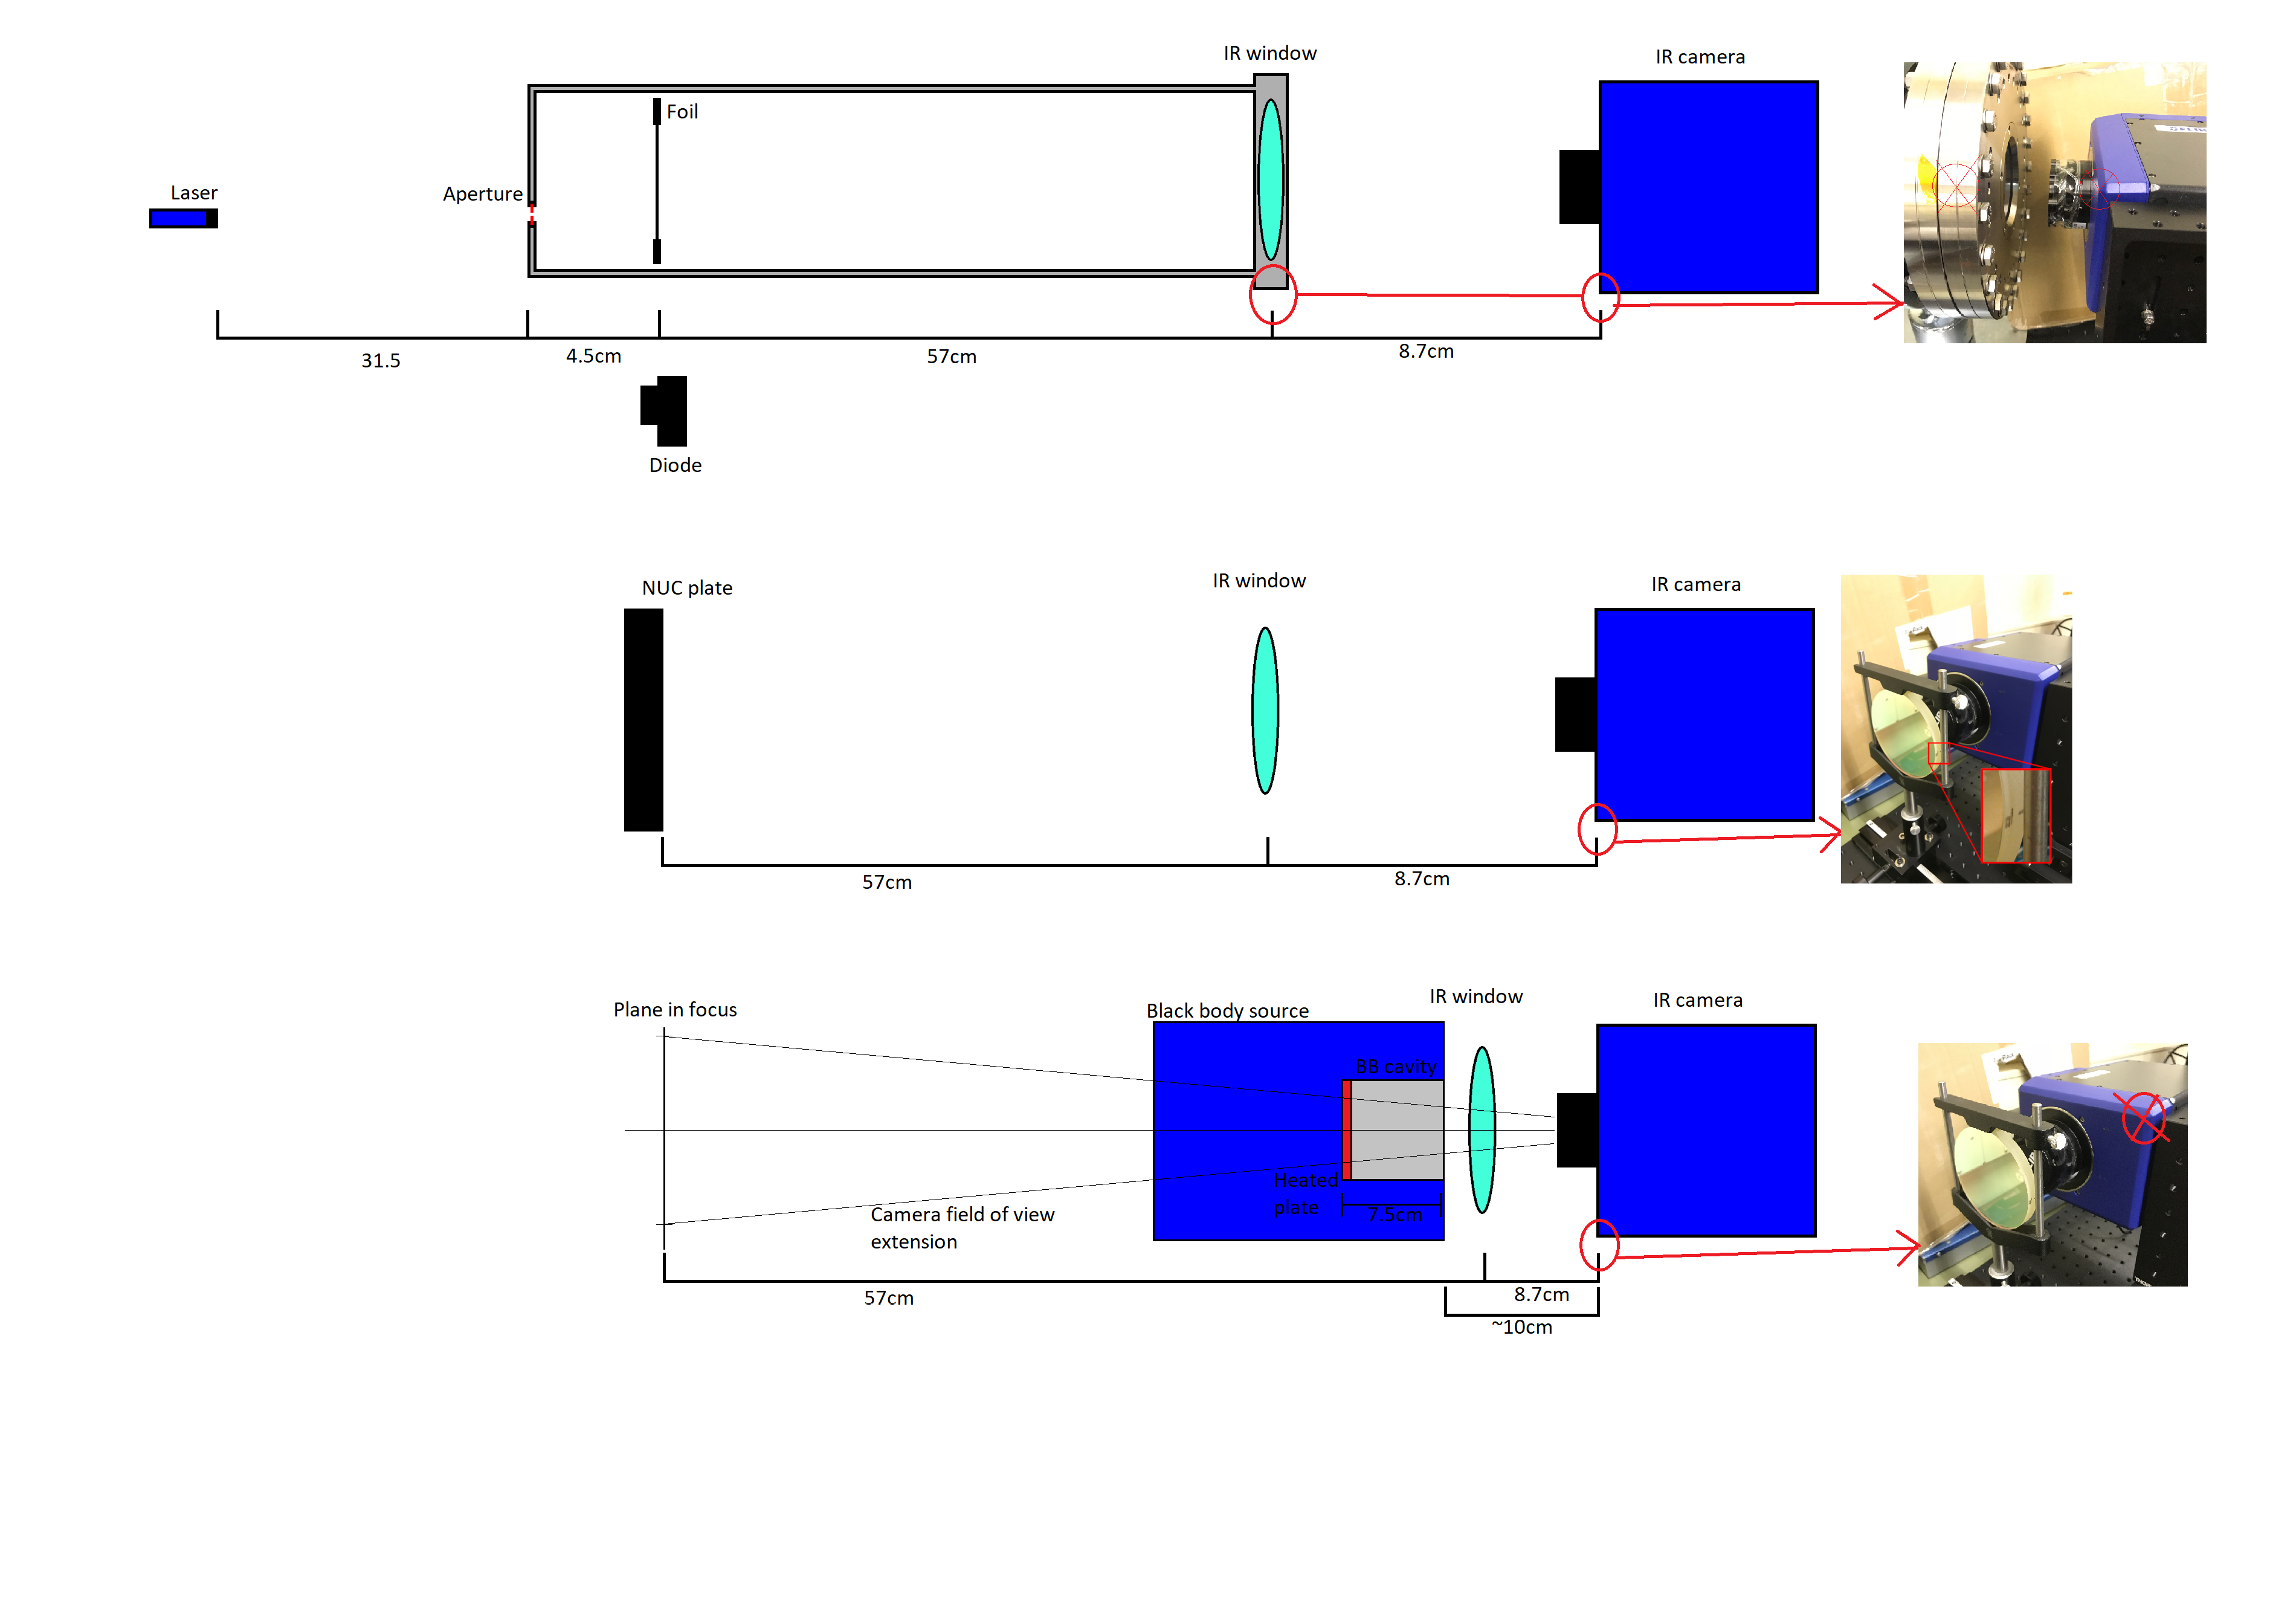
\includegraphics[trim={780 850 280 700},clip,width=\linewidth]{Chapters/chapter2/figs/calib_schematics.png}
	\caption{Schematic of the calibration setup. The NUC plate and the IR window are located at the same distance from the camera as when installed and as per design. Effort is made to keep the window with the same rotational orientation. See the marking for the view port alignment in the detail.}
	\label{fig:BBcalib}
\end{figure*}

The geometry of the calibration is represented in \autoref{fig:BBcalib}. The relative distances are the same as when the camera is installed. The rotational orientation of the view port was maintained during calibration and on the machine thanks to markings on the side of the window. During testing the narcissus effect was clearly observed.

\begin{figure}[!ht]
     \centering
     \begin{subfigure}{0.435\linewidth}
         \centering
         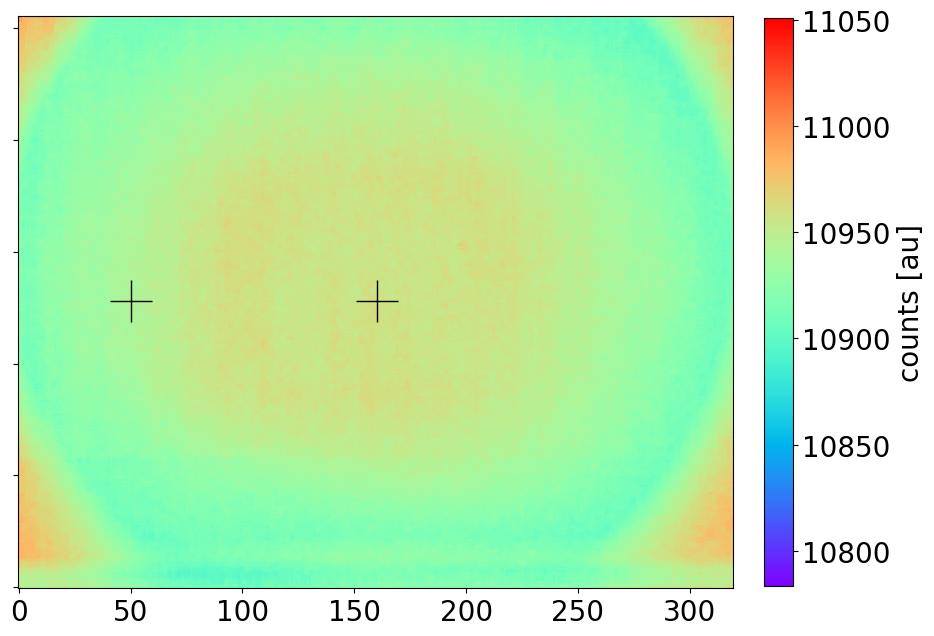
\includegraphics[trim={5 0 130 5},clip,width=\linewidth]{Chapters/chapter2/figs/NUC_calib2.png}
         \caption{}
         \label{NUC_calib2}
     \end{subfigure}
     \begin{subfigure}{0.535\linewidth}
         \centering
         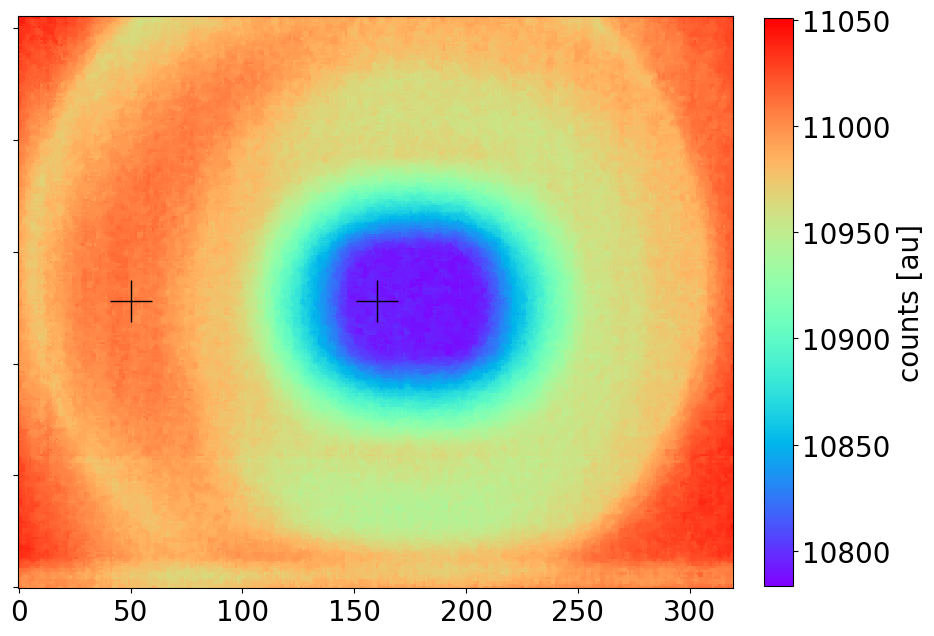
\includegraphics[trim={5 0 5 5},clip,width=\linewidth]{Chapters/chapter2/figs/NUC_calib1.png}
         \caption{}
         \label{NUC_calib1}
     \end{subfigure}
     \begin{subfigure}{0.7\linewidth}
         \centering
         \includegraphics[trim={120 0 15 63},clip,width=\linewidth]{Chapters/chapter2/figs/IRVB-MASTU_shot-45473_foil_fit.eps}
         \caption{}
         \label{foil_fit}
     \end{subfigure}
    \caption{Example of non uniformity of the counts of the IR camera when aimed at the NUC plate at room temperature. Shown are the images without the view port (\subref{NUC_calib2}) and with (\subref{NUC_calib1}). The same scale is applied to both plots and there was a 2ms integration time. The black cross indicates two reference points (inside/outside the narcissus) that will be used in later analysis. \subref{foil_fit} shows the position of the foil (the red square) inside the camera field of view. Around the foil are the bolts that lock the foil in between the two copper plates, that can be used to identify the foil orientation.}
    \label{fig:NUC1}
\end{figure}

\autoref{fig:NUC1} displays the qualitative effect of the presence of the view port. \autoref{NUC_calib2} shows the typical view when the camera images the NUC plate; vignetting due to the camera lenses is apparent. \autoref{NUC_calib1} shows the effect of the window reflections. In \autoref{foil_fit} the effect on the foil image is shown. The dark spot caused by the narcissus is at the centre of the image, decreasing the counts by $\sim$200 counts at an integration time of $2ms$. This should be a systematic error and, therefore, should mostly impact the $a_2$ coefficient that ultimately doesn't impact the temperature measurement.
During the temperature ramps it was observed that the NUC plate, albeit having a uniform emissivity, shows a non uniform temperature across the FOV due to heat transfer. The plate is naturally cooled/heated via conduction, convection and black body radiation. Air flows around the plate and can lead to uneven heat transport.

\begin{figure}[!ht]
     \centering
     \begin{subfigure}{0.7\linewidth}
         \centering
         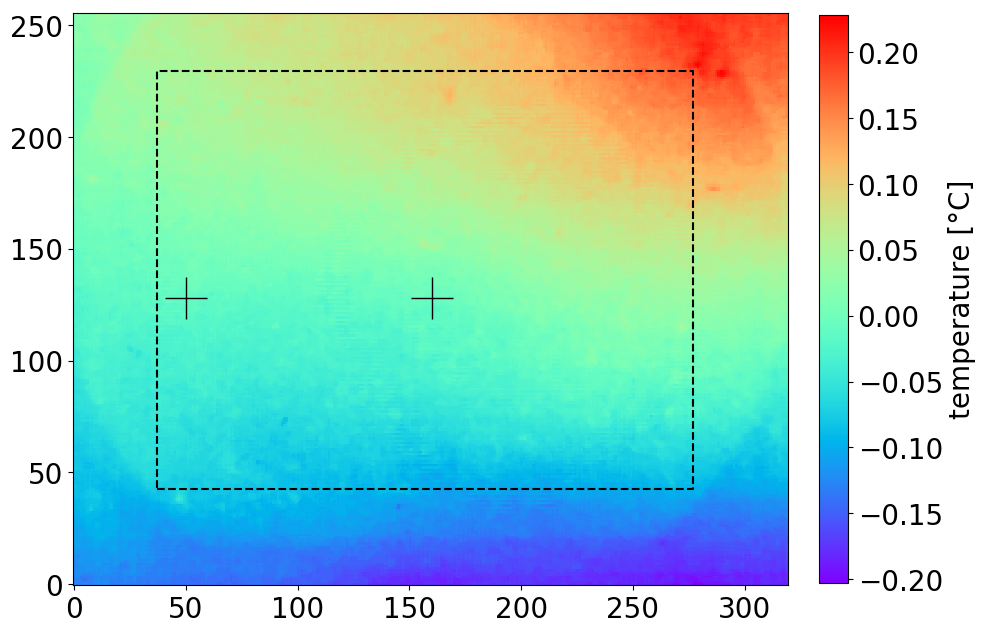
\includegraphics[trim={0 0 0 0},clip,width=\linewidth]{Chapters/chapter2/figs/NUC_calib6.png}
         \caption{}
         \label{NUC_calib6}
     \end{subfigure}
     \begin{subfigure}{0.7\linewidth}
         \centering
         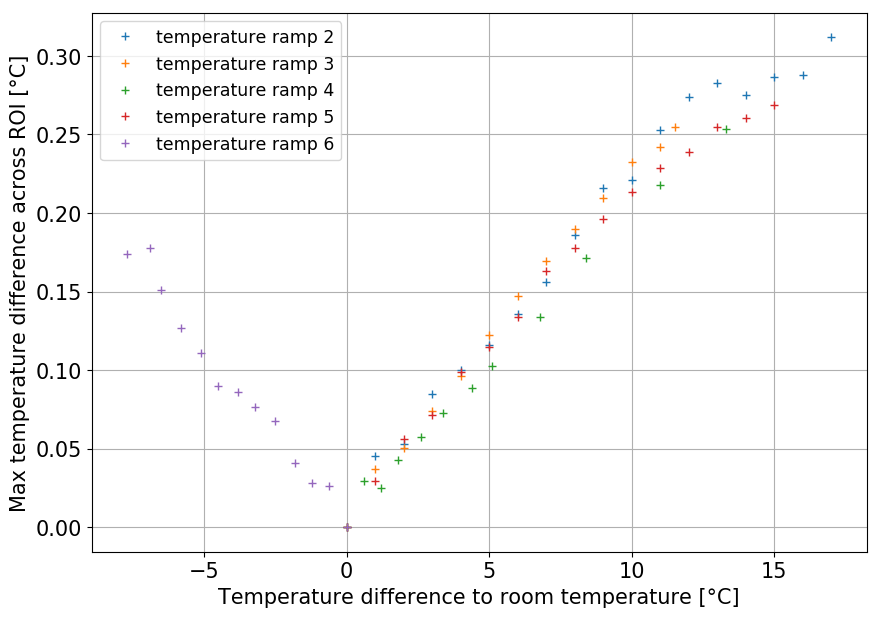
\includegraphics[trim={0 0 5 0},clip,width=\linewidth]{Chapters/chapter2/figs/NUC_calib5.png}
         \caption{}
         \label{NUC_calib5}
     \end{subfigure}
    \caption{(\subref{NUC_calib6}) Shown are the IR camera counts at $41.9\degree C$ minus the counts at room temperature, scaled up such that the average across the foil is the same as at high temperature. In black is highlighted the region corresponding approximately to the IRVB foil and the two reference points defined in \autoref{fig:NUC1}. The vertical orientation is here bottom to top, with the top of the image being up. (\subref{NUC_calib5}) Peak temperature difference between the temperature deriving from the counts at high temperature and the counts at room temperature scaled up as previously mentioned.}
    \label{fig:NUC2}
\end{figure}

The temperature non uniformity across the image was estimated for different temperature ramps as shown in \autoref{NUC_calib5} and it was found to be at most $0.3\degree C$ on average in the temperature range of interest. As shown in \autoref{NUC_calib6} the spatial variation of temperature is very slow, with a very minor impact on the spatial and temporal derivative. The effect of the location where the thermocouple is connected to the NUC plate was also investigated by moving it to different corners of the plate. The spread of the temperature around a curve that fits average camera counts and temperature for all the probe positions with the model in \autoref{Counts to temperature model} is about $0.25\degree C$. There was, though, no pattern found so the difference is most likely due to the connection of the sensor to the plate rather than the actual temperature of the plate.

\begin{figure}[!ht]
     \centering
     \begin{subfigure}{0.7\linewidth}
         \centering
         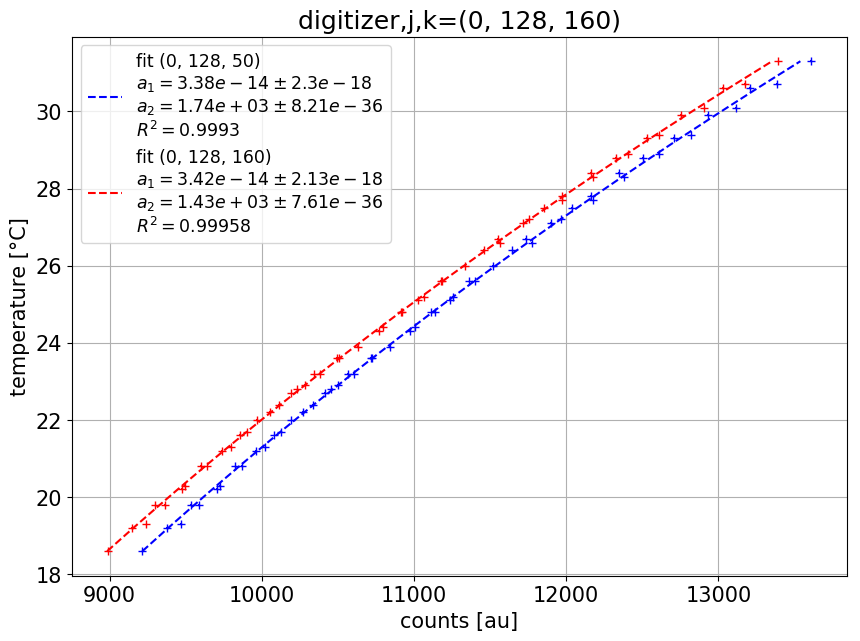
\includegraphics[trim={5 0 0 25},clip,width=\linewidth]{Chapters/chapter2/figs/example_BB_fit(0, 128, 160)2.png}
     \end{subfigure}
    \caption{Comparison of the temperature calibration curves for a pixel at the centre of the narcissus (red) with one on its side (blue). The legend gives the fit parameters ($a_1$ proportional and $a_2$ additive components), their uncertainties, and the coefficient of determination of the fit.}
    \label{fig:example_BB_fit}
\end{figure}

The result of the scan for the two pixels identified in \autoref{fig:NUC1}, one close to the centre of the narcissus effect and one on its side, are shown in \autoref{fig:example_BB_fit}. \autoref{eq:BBphotons3} can reproduce the measurements with high accuracy. As expected the presence of the narcissus mostly affects the $a_2$ offset.

The results of the calibration for the entire foil are shown in \autoref{fig:NUC_a1_a2}. Both coefficients are affected by vignetting and the narcissus effect. It is noteworthy that the $\sim$200 counts at the centre of the narcissus are assigned entirely to the constant parameter, as one would expect for a systematic error. Some of the variation in $a_1$, especially the red ring around the centre, could be related to the narcissus, meaning that its effect is not completely independent of temperature. The variation in $a_1$ is very small, however, only $\sim$2\% and changes fairly slowly across the FOV, resulting in a small impact on the spatial and temporal temperature derivatives. Both coefficients seem to have a general dependency on the vertical direction (right to left in the figure), possibly due to the slight non-uniformity of the temperature of the NUC plate.

\begin{figure}[!ht]
     \centering
     \begin{subfigure}{0.6\linewidth}
         \centering
	    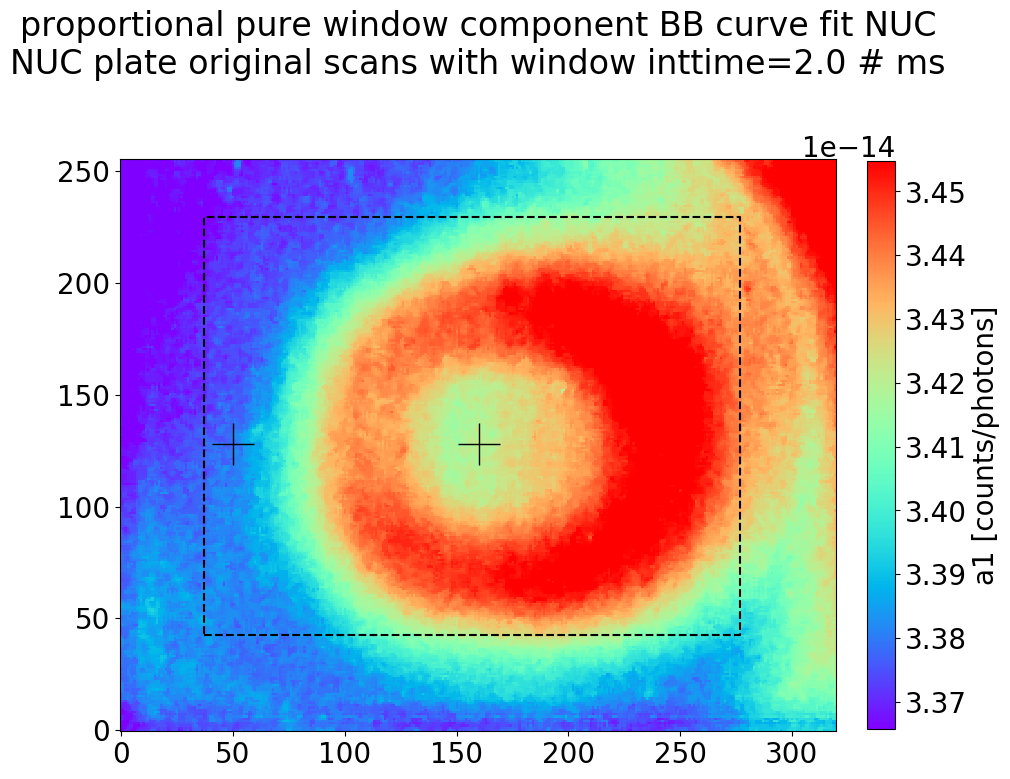
\includegraphics[trim={40 0 0 60},clip,width=\linewidth]{Chapters/chapter2/figs/NUC_a12.png}
         \phantomcaption{$a_1$}
         \label{NUC_a1}
     \end{subfigure}
     \begin{subfigure}{0.6\linewidth}
         \centering
    	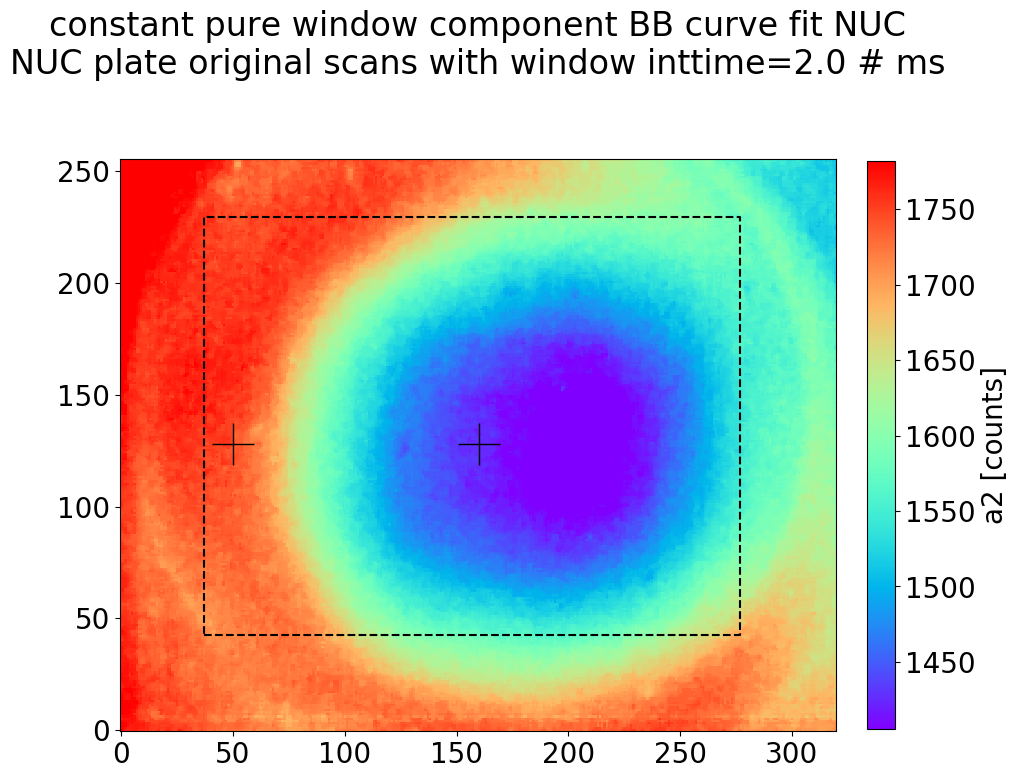
\includegraphics[trim={40 0 0 60},clip,width=\linewidth]{Chapters/chapter2/figs/NUC_a22.png}
         \phantomcaption{$a_2$}
         \label{NUC_a2}
     \end{subfigure}
    \caption{$a_1$ and $a_2$ coefficients of \autoref{eq:BBphotons3} obtained via calibration with the NUC plate. In black is highlighted the region corresponding approximately to the IRVB foil and the two reference points defined in \autoref{fig:NUC1}. The vertical orientation during this calibration is right to left, with the top on the left.}
    \label{fig:NUC_a1_a2}
\end{figure}

For future calibrations, a large flat black body calibration source with the capability to cool below and heat above room temperature could be used to further reduce the uncertainties in the NUC plate temperature. 

\subsection{Foil model}\label{Foil model}
The foil thermal response is dictated by heat transport: the source is the radiated power from the plasma reaching the foil ($P_{foil}$) while the local sinks are its black body radiation ($P_{BB}$), conduction ($P_{\Delta T}$) and temperature variation ($P_{\frac {\partial T} {\partial t}}$). The foil is very thin and therefore 2D heat transport can safely be considered instead of 3D. \autoref{eq:heat2d} shows how to calculate the power absorbed by the foil based on its temperature.

\begin{equation}
\label{eq:heat2d}
\begin{aligned}
P_{foil}=& P_{\frac {\partial T} {\partial t}}+P_{\Delta T}+P_{BB}\\
P_{\frac {\partial T} {\partial t}}=& \dfrac{k \: t_f}{\kappa} \dfrac{dT}{dt} \\
 P_{\Delta T} =& -k \: t_f \:  \left( \dfrac{\partial^2 T}{\partial x^2} + \dfrac{\partial^2 T}{\partial y^2} \right) \approx -k \: t_f \: L \cdot T \\ P_{BB} =& 2 \: \varepsilon \: \sigma_{SB} \: (T^4 - T_0^4)
\end{aligned}
\end{equation}

where $k$ is the thermal conductivity, $t_f$ the thickness, $\kappa$ the thermal diffusivity, $\varepsilon$ the black body emissivity and $\sigma_{SB}$ the Stefan-Boltzmann constant. $L$ is the matrix containing the coefficients to build the temperature Laplacian via the dot product. It is built such that its dot product with the temperature returns the sum of the second order central finite difference in all directions. In the Laplacian matrix the elements corresponding to the derivative in the diagonal direction are divided by 2, to account for the increase in distance.

Assuming $\alpha(T)$ to be slowly varying the uncertainty in the temporal variation, diffusion and radiation terms of the heat equation can be calculated with Equations \ref{eq:uncert1}, \ref{eq:uncert2} and \ref{eq:uncert3} respectively for the pixel $i$:
\begin{equation}
{\sigma }_{ \frac {\partial T} {\partial t}} = \frac{k \: t_f}{\kappa \: dt}  \sqrt{ \left ( \frac {{\sigma }_{C_{i+1}}} { a_1 \alpha(T_{i+1}) } \right )^2 + \left ( \frac {{\sigma }_{C_{i-1}}} { a_1 \alpha(T_{i-1}) } \right )^2 + \left [ \left ( T_{i+1}-T_{i-1} \right ) \frac {{\sigma }_{a_1}} {a_1} \right ]^2 } 
\label{eq:uncert1}
\end{equation}
\begin{equation}
{\sigma }_{ \Delta T} = \frac {k \: t_f} {dx^2} \sqrt{ L^2 \cdot \left[  \left(  \frac {{\sigma }_{C_i}} { a_1 \alpha(T_i) } \right)^2 + \left( \frac {{\sigma }_{C_0}} { a_1 \alpha(T_0) } \right)^2 + \left( ({T_i -T_0}) \frac {{\sigma }_{a_1}} {a_1} \right)^2 \right] } 
\label{eq:uncert2}
\end{equation}
\begin{equation}
\begin{aligned}
{\sigma }_{T_i} =& \frac 1 {\alpha(T_i)} \sqrt{ \frac {({\sigma }_{C_i}^2 + {\sigma }_{C_0}^2 )} { a_1^2 } + \left [ \left (\frac {C_i -C_0} {a_1} \right ) \frac {{\sigma }_{a_1}} {a_1} \right ]^2  + (\alpha(T_i) {\sigma }_{T_0})^2 } \\ {\sigma }_{ BB} =& 4 \: \varepsilon \: \sigma_{SB} \sqrt{ ({T_i}^3 {\sigma }_{T_i})^2 + ({T_0}^3 {\sigma }_{T_0})^2 }
\label{eq:uncert3}
\end{aligned}
\end{equation}

\subsection{Foil calibration}\label{Foil calibration}
In this section the calibration procedure followed to obtain the foil properties will be detailed. To calibrate the foil its thickness $t_f$, thermal $\kappa$ diffusivity and black body emissivity $\varepsilon$ must be determined (assuming nominal Platinum thermal conductivity $k=71.6W/mK$). A set of spatially resolved parameters was supplied together with the foil of which the average and variability across the foil corresponds to ${\epsilon=0.85\pm0.04}, {t_f=1.29\pm0.17 \mu m}$. Nominal platinum thermal diffusivity is assumed ${\kappa=2.5\;10^{-5}m^2/s}$. These values were obtained with a single exposure of a laser of known power, pulse and and spatial shape by monitoring the cooling down phase of the foil in vacuum as described in \cite{Itomi2014}. There are different ways to find the foil parameters, all reliant on shining a laser on the foil (see references \cite{Sano2012,Itomi2014,Cernuschi2001}).

Rather than using a single laser exposure, the method of choice relied upon varying the laser intensity, frequency and focus as done by Reinke.\cite{Reinke2018a} With slow pulses, the time variation component tends to become irrelevant such that only black body radiation and diffusion remain. With a defocused laser (low laser power density), the temperature increase is low and the spatial distribution slowly varying, increasing the relevance of the black body radiation. With a fast pulsed laser the time dependent component is dominant.


\begin{figure}[!ht]
     \centering
     \begin{subfigure}{0.8\linewidth}
        \centering
        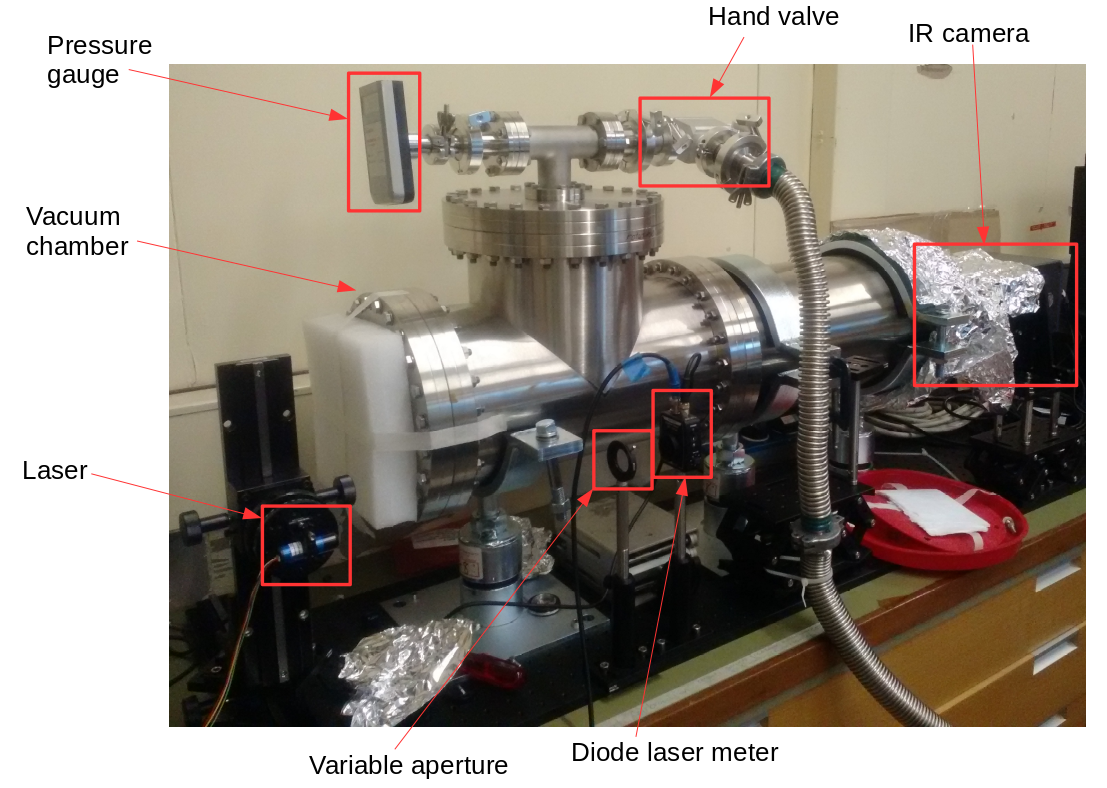
\includegraphics[width=\textwidth,trim={20 0 20 0},clip]{Chapters/chapter2/figs/vacuum_setup_3.png}
        \vspace*{-5mm}
        {\color{white}\caption{\phantom{ }}\label{fig:vacuum_setup1}}
        %  \caption{\phantom{}}
        %  \label{fig:MAST-U_HFS_MID_L08_1}
     \end{subfigure}
     \begin{subfigure}{0.8\linewidth}
        \centering
        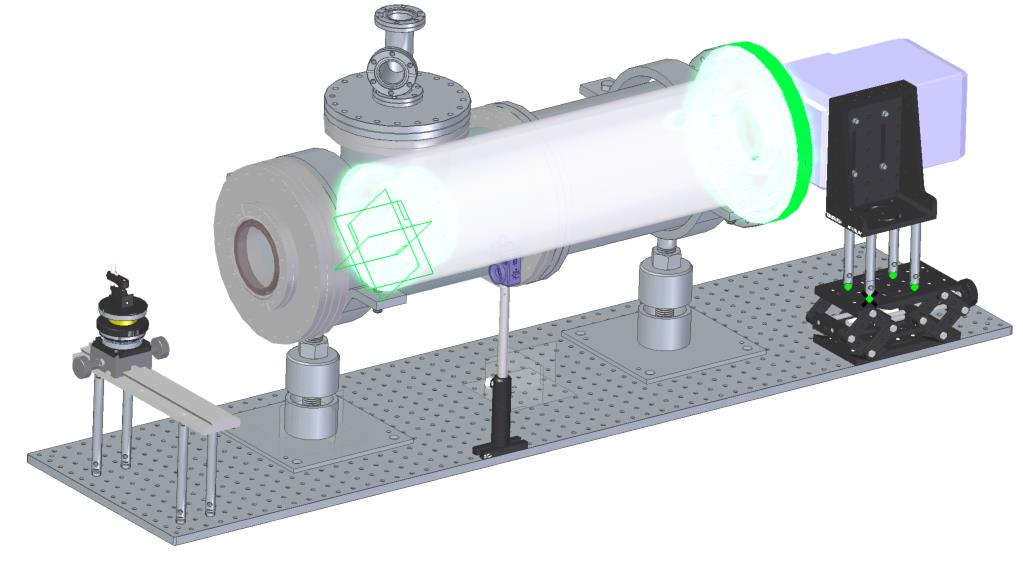
\includegraphics[width=\textwidth,trim={0 0 0 0},clip]{Chapters/chapter2/figs/vacuum_setup2.png}
        \vspace*{-5mm}
        {\color{white}\caption{\phantom{ }}\label{fig:vacuum_setup2}}
        %  \caption{\phantom{}}
        %  \label{fig:vacuum_setup2}
     \end{subfigure}
        \vspace*{+5mm}
        \caption{Photograph (\subref{fig:vacuum_setup1}) and CAD model (\subref{fig:vacuum_setup2}) of the bench-top setup used for the foil calibration. In the CAD model the re-entrant tube is shown in white and the foil assembly is on the left side. The photograph, taken on 02/08/2018, shows the laser used to illuminate the foil, as well as the diode and aperture used to calibrate the laser and vacuum system.}
        \label{fig:vacuum_setup}
\end{figure}


A bench top vacuum system was built for the foil calibration, shown in \autoref{fig:vacuum_setup}. The vacuum is necessary to eliminate convection as a heat loss mechanism, as it is also absent during the experiments. The pressure during calibration was $\sim 3 \cdot 10^{-5}bar$, compared to $\sim 10^{-8}bar$ during MAST-U experiments.
%\hl{Matt has a plot to compare pressure and effect on calibration, ask the reference} 
A $5mW, 655nm$ BlueLyte laser was used, capable of gradually reducing the total power output to zero and with a maximum modulation up to 750kHz. The laser was equipped with an adjustable lens to change the focus. The laser was calibrated with a Thorlabs PDA100A2 diode in combination with a variable aperture. The maximum laser intensity was measured to be about $1200W/m^2$ and $50W/m^2$ when focused and defocused respectively, with a maximum total power of 4.16mW. The laser was controlled with a square wave function generator so that the laser output was modulated in intensity, frequency and focus. The transmission of the vacuum window on the laser side was measured at $93.3\%$ and taken into account. The power delivered to the foil integrated over the pinhole area, $P$, can be determined with \autoref{eq:heat2d}. To find the foil thermal properties, the running average of $P$ is computed, averaging over the duration of half the square wave duration. The peaks $P_h$ and troughs $P_l$ of the running average are compared to the input values $P_{in}$.
% Additionally a measure of the squareness of the found power profile given by \autoref{eq:squareness}. The denominator is a proxy for the standard deviation but that it is almost insensitive of the shape of the wave.

% \begin{equation}
% SQ = \frac{std \left (P \left [P>P_l+\frac{P_h-P_l}{2} \right ] \right ) + std \left (P \left [P<P_l+\frac{P_h-P_l}{2} \right ] \right )}{\sqrt{mean((P[1:]-P[:-1])^2)}}
% \label{eq:squareness}
% \end{equation}

A scan in laser power from 0 to 100\% and frequency from 0.2 to 90Hz with the laser fully focused and fully defocused was carried out in the location of the foil closer to the pinhole. The fit was done with data up to 10Hz returning the following fit parameters: ${\epsilon=1}, {t_f=2.69\mu m}, {\kappa=1.35\;10^{-5}m^2/s}$. The $t_f / \kappa$ ratio is similar to foil properties measured prior to the installation on NSTX-U, differing significantly from the supplied one.\cite{Reinke2018} The difference in the $t_f$ and $\kappa$ values is likely due to the difference in emissivity inferred.

\begin{figure}[!ht]
     \centering
     \begin{subfigure}{0.6\linewidth}
        \centering
        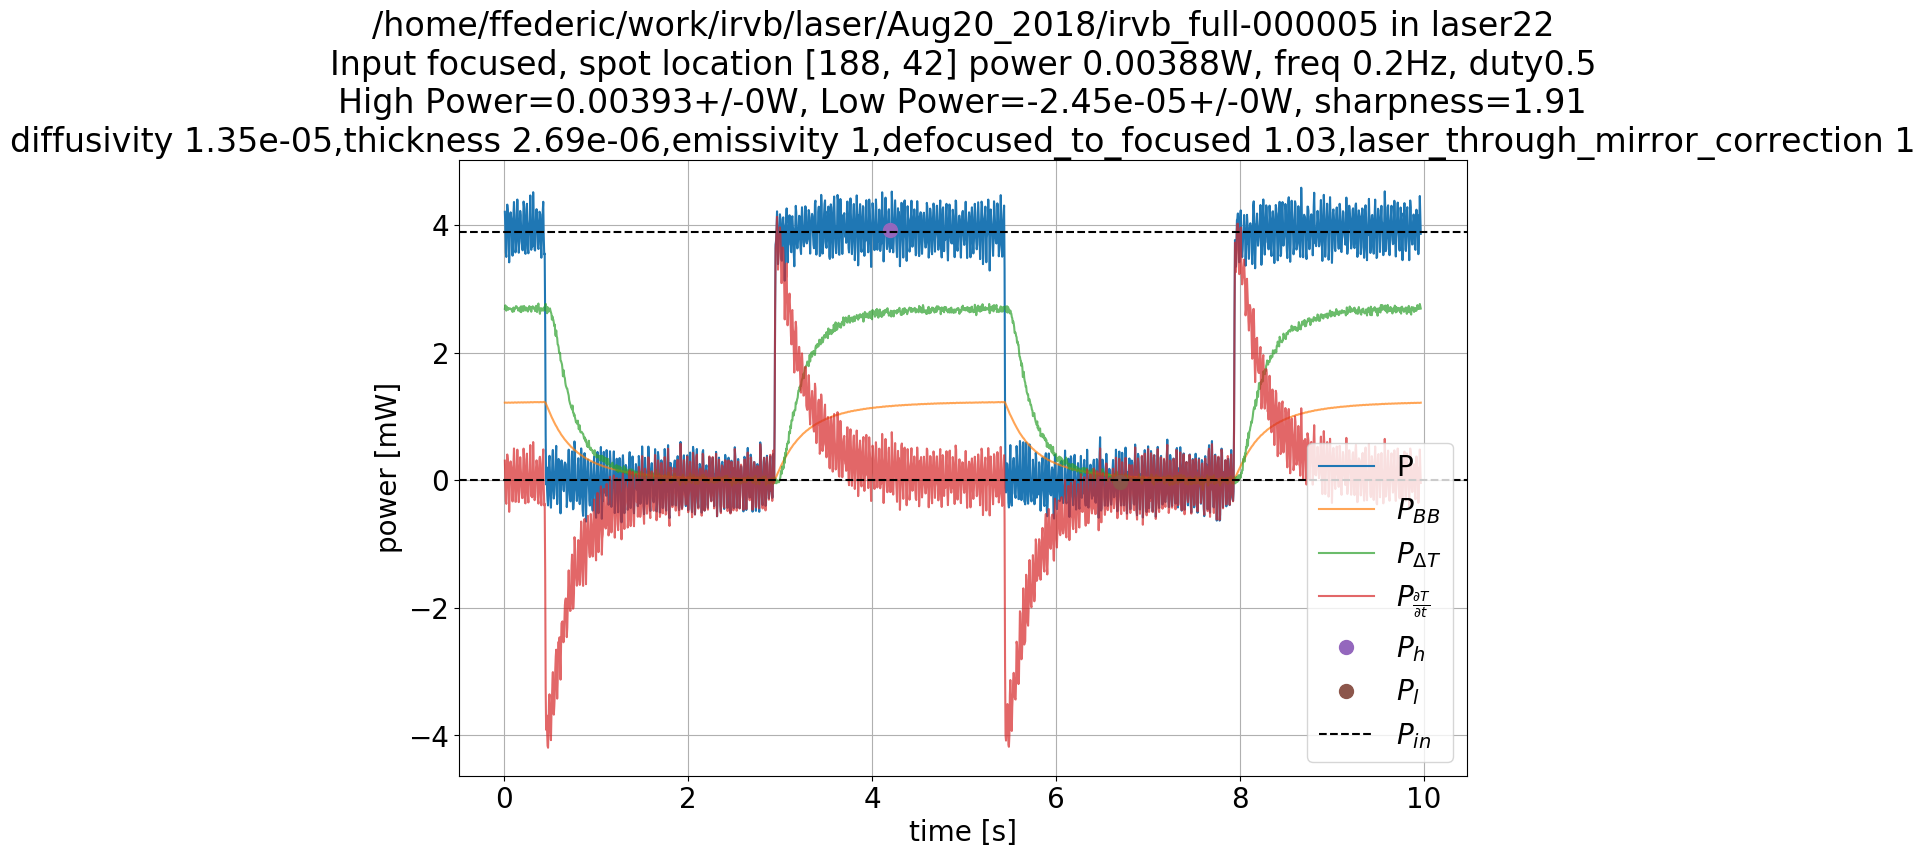
\includegraphics[width=\textwidth,trim={270 0 320 115},clip]{Chapters/chapter2/figs/example_for_paper_22.png}
        \vspace*{-5mm}
        {\color{white}\caption{\phantom{ }}\label{fig:example_for_paper_15}}
        %  \caption{\phantom{}}
        %  \label{fig:MAST-U_HFS_MID_L08_1}
     \end{subfigure}
     \begin{subfigure}{0.6\linewidth}
        \centering
        \includegraphics[width=\textwidth,trim={270 0 320 115},clip]{Chapters/chapter2/figs/example_for_paper_23.png}
        \vspace*{-5mm}
        {\color{white}\caption{\phantom{ }}\label{fig:example_for_paper_14}}
        %  \caption{\phantom{}}
        %  \label{fig:vacuum_setup2}
     \end{subfigure}
     \begin{subfigure}{0.62\linewidth}
        \centering
        \includegraphics[width=\textwidth,trim={250 0 320 115},clip]{Chapters/chapter2/figs/example_for_paper_21.png}
        \vspace*{-5mm}
        {\color{white}\caption{\phantom{ }}\label{fig:example_for_paper_12}}
        %  \caption{\phantom{}}
        %  \label{fig:vacuum_setup2}
     \end{subfigure}
        % \vspace*{+5mm}
        \caption{Examples of the power absorbed by the foil and its components (total absorbed power $P$ and its components black body radiation $P_{BB}$, conduction $P_{\Delta T}$ and temperature variation $P_{\frac {\partial T} {\partial t}}$; peaks and troughs of $P$ running average, $P_h$ and $P_l$; peak input power $P_{in}$) with the laser at maximum intensity for a focused low frequency case (\subref{fig:example_for_paper_15}), a focused high frequency case (\subref{fig:example_for_paper_14}) and a defocused low frequency one (\subref{fig:example_for_paper_12}).}
        \label{fig:example_for_paper_1}
\end{figure}

\begin{figure}[!ht]
	\centering
	\includegraphics[trim={290 0 330 100},clip,width=0.65\linewidth]{Chapters/chapter2/figs/example_for_paper_24.png}
	\caption{Variation of the measured power compared to the expected values with laser intensity (top) and frequency (bottom). The blue color indicates the defocused cases while the red the focused ones. $P_h$ and $P_l$ are the inferred high and low power level of the laser square wave, $area$ is the area of the foil receiving laser light, $P_{in}$ is the known peak laser power density.}
	\label{fig:example_for_paper_2}
\end{figure}

An example of the power calculated in the laser experiments is shown in \autoref{fig:example_for_paper_1} while \autoref{fig:example_for_paper_2} shows the quality of the fit for varying power and frequency and for focused and defocused laser light. It can be observed that above 30Hz the inferred power drops, implying a limit in the temporal resolution of the IRVB. The data corresponding to the defocused laser degrades at lower frequencies, as the total delivered laser power is lower. During these experiments it was also observed that a fixed oscillation of $0.01K$ at about $29Hz$ is superimposed on the data so measurements at the same frequency or higher will be affected. The oscillation seems to be independent of the power supply system and the frame rate but proportional to the integration time, ultimately due to the internal operation of the camera.


These foil properties were measured in a single location and were therefore assumed uniform across the foil. To account for the variability across the foil the uncertainty from the fit is increased by the variability of the properties provided to us with the foil. This returns the uncertainties ${\sigma_{\epsilon}/\epsilon=8.61\%}, {\sigma_{t_f}/t_f=13.6\%}, {\sigma_{\kappa}/\kappa=13.9\%}$ (for $\kappa$ is used the same variability across the foil as for $t_f$).

\subsection{Etendue}\label{Etendue}
In order to convert the measurement from the power absorbed by the foil to the brightness at the pinhole, the geometrical configuration of the foil compared to the pinhole has to be considered. This is given by the etendue, that it is calculated here for the section of the foil corresponding to the $(i,j)$ pixel of the IR camera with the simplified formulation in \autoref{eq:etendue} \cite{Reinke2011,Carr2018}

\begin{equation}
U_{i,j} = \frac{A_{i,j} A_{pin} cos(\psi) cos(\phi)}{d_{i,j}^2}
\label{eq:etendue}
\end{equation}

Where $A_{i,j}$ is the area of the pixel, $A_{pin}$ is the area of the pinhole, $d_{i,j}$ is the distance from the centre of the pinhole to the pixel and $\psi$ and $\phi$ are the angle from the normal to the pinhole to the vector from pinhole to pixel and the angle from the normal to the pixel to the vector from pixel to pinhole respectively. $A_{i,j}$ is considered equal for all pixels ($A_pix$) and is given by the size of the foil as seen from the camera. As it can be seen in \autoref{fig:IRVB3} the foil is parallel to the aperture therefore $cos(\psi) = cos(\phi) = d_{fp}/d_{i,j}$ where $d_{fp}$ is the minimum distance from the pinhole to the foil. \autoref{eq:etendue} reduces then to \autoref{eq:etendue2}.

\begin{equation}
U_{i,j} = \frac{A_{pix} A_{pin} d_{fp}^2}{d_{i,j}^4}
\label{eq:etendue2}
\end{equation}

The brightness is then simply obtained with \autoref{eq:etendue3}.

\begin{equation}
B = P_{foil}\frac{4\pi}{U}
\label{eq:etendue3}
\end{equation}



\subsection{Viewing geometry validation}

The viewing geometry of the diagnostic as designed in \autoref{MAST-U IRVB design} has to be validated to make sure that each IRVB pixel FOV into the plasma is as expected. For diagnostics where a camera is directly imaging inside the vacuum vessel this is usually done by acquiring long exposure images and matching the observed features on the machine surface with features from CAD models. For bolometers this is not possible as the black body radiation of the vessel surfaces is many orders of magnitude below the detection limit, even when heated up by the plasma. For this reason this spatial calibration has to rely on laser light sources. The size and orientation of the LOS viewing cone is often measured in dedicated laboratory experiments and translated into machine coordinates using some reference point of the diagnostic assembly and the vessel.\cite{McCormick2005,Huber2007} If there is good access to the inside of the machine, a laser can be placed in fixed locations to measure the bounds of the light detection region of every LOS.\cite{Reinke2011} More recently, in the effort to develop the bolometer system for ITER, a robotic arm was developed on AUG which can probe the relation between the origin of the emission and sensor response by moving a laser to various positions in the field of view of the bolometer.\cite{Penzel2014} An inability to access the interior of MAST-U prevented these types of measurements. For these reasons the geometry of the IRVB was verified by comparing known features of the plasma during operation with their expected locations, adapting methods used for visible imaging. The bright features of interest are fueling locations, alignment of the center-column and the flash heating of the foil from disruptions.

\subsubsection{Spatial calibration using fueling valves and EFIT++}\label{Spatial calibration using fueling valves and EFIT++}

% \begin{figure}[!ht]
% 	\centering
% 	\includegraphics[trim={0 0 0 0},clip,width=\linewidth]{Chapters/chapter2/figs/Mast_u_gas_valves.jpg}
% 	\caption{Poloidal cross section of the lower half of MAST-U indicating the location of the fuelling inlets and relative naming. The inlets are symmetric above the below midplane and for each a series of them are toroidally distributed. Only a limited fraction of the gas valves was available for MU01. \cite{McArdle2020}}
% 	\label{fig:MAST-U_valves}
% \end{figure}

% \begin{figure}[!ht]
% 	\centering
% 	\includegraphics[trim={40 0 25 10},clip,width=\linewidth]{Chapters/chapter2/figs/Mast_u_gas_valves_2.png}
% 	\caption{Schematic of the fuelling piping for the lower half of MAST-U. The names correspond to the only valves that the IRVB can directly image. \cite{Hawkins2022}}
% 	\label{fig:MAST-U_valves2}
% \end{figure}

The plasma can be fuelled via a multitude of entry ports, of which only some are directly visible by the IRVB. The names of the valves corresponding to the visible outlets are indicated in \autoref{fig:calcam}. %Of the gas fuelling valves with outlets in the FOV, HFS\_MID\_L02 was not available during the MU01 campaign. 
If hot plasma is present in the immediate vicinity of the gas outlet, the hot electrons dissociate and then excite and ionise the injected neutrals. If the electron temperature is not too high and the plasma is close enough, a bright non-toroidally-symmetric emission appears in the vicinity of the gas outlet. In all the observed discharges when the gas injection valve PFR\_BOT\_B01 was employed, a localised bright region never appeared, possibly because the separatrix was too far away or the gas flow too low. The fuelling valves, then, that caused a visible localised emission to appear in the IRVB FOV are HFS\_MID\_L08 and HFS\_BOT\_B03, although HFS\_BOT\_B03 was only used once and thus not very useful to compare across pulses.

% \begin{figure}[!ht]
% 	\centering
% 	\includegraphics[trim={0 0 0 15},clip,width=\linewidth]{Chapters/chapter2/figs/IRVB-MASTU_shot-44647_export_1.png}
% 	\caption{Example of the radiation spot caused by the valve HFS\_BOT\_B03 (marked by a black cross and a violet arrow) from shot 44647. The brightness data is obtained by binning the temperature profile, solving the heat equation and dividing by the etendue. In dashed blue the poloidal projection of the separatrix. In solid red the toroidal trace of x-point and strike points and in dashed red the magnetic axis. The radiation appear in the closer location on the separatrix from the valve location.}
% 	\label{fig:MAST-U_HFS_BOT_B03}
% \end{figure}

%The valve HFS\_BOT\_B03 was activated only once in MU01 for the early shot 44647 so it is not possible to verify if the emission appears consistently across multiple shots. It must be noted that during MU01 there was no feedback of the actual flow rate from the valves, so the proper operation of the valve is not certain. Emission from the gas injected by the valve cannot be conclusively identified with the IRVB and the outlet is not in the field of view of any other diagnostic, so this data is omitted. 
% In \autoref{fig:MAST-U_HFS_BOT_B03} is shown the brightness resulting by the gas injected by the valve. The radiation is clearly non toroidally symmetric and comes from a region with sufficiently high plasma density and temperature and still close to the injection point. This happens in the vicinity of the separatrix, whose poloidal projection is indicated in dashed blue. The radiation induced by this valve cannot be verified with other diagnostics, as no other has LOS at this toroidal and poloidal location.

The 2 HFS\_MID\_L08 valve outlets locations at the inner wall can be used as one spatial calibration of the IRVB viewing geometry. The valve is consistently used throughout MU01 and its outlets are both in the field of view of the high speed visible light camera (HSV), shown in \autoref{fig:HSV1}, while only one outlet is in the IRVB FOV. Strong visible light brightness does not necessarily indicate a strong total radiated power, but indicates regions where neutral hydrogen is interacting with the plasma.\cite{Walkden2017}

\begin{figure}[!ht]
	\centering
	\includegraphics[width=0.6\linewidth,trim={0 0 0 0},clip]{Chapters/chapter2/figs/hsv_FOV2.png}
	\caption{Field of view of the high speed visible light camera indicating the sector numbers. In yellow the locations of the outlets of the gas valve HFS\_MID\_L08 are indicated. In red is shown the location of the outlets of the gas valve HFS\_MID\_U02, dashed because they are on the other side of the central column, hidden from view.}
	\label{fig:HSV1}
\end{figure}


\begin{figure}[!ht]
     \centering
     \begin{subfigure}{0.48\linewidth}
        \centering
        \includegraphics[width=\textwidth,trim={15 10 0 20},clip]{Chapters/chapter2/figs/IRVB-MASTU_shot-45295_export_4.png}
        \vspace*{-6mm}
        {\color{white}\caption{\phantom{ }}\label{fig:MAST-U_HFS_MID_L08_1}}
        %  \caption{\phantom{}}
        %  \label{fig:MAST-U_HFS_MID_L08_1}
     \end{subfigure}
     \begin{subfigure}{0.48\linewidth}
        \vspace*{2mm}
        \centering
        \includegraphics[width=\textwidth,trim={55 41 0 50},clip]{Chapters/chapter2/figs/45295_for_paper3.png}
        \vspace*{-6mm}
        {\color{white}\caption{\phantom{ }}\label{fig:MAST-U_HFS_MID_L08_2}}
        %  \caption{\phantom{}}
        %  \label{fig:MAST-U_HFS_MID_L08_2}
     \end{subfigure}
     \begin{subfigure}{0.6\linewidth}
        \vspace*{2mm}
        \centering
        \includegraphics[width=\textwidth,trim={5 0 0 0},clip]{Chapters/chapter2/figs/45295_for_paper2.png}
        \vspace*{-6mm}
        {\color{white}\caption{\phantom{ }}\label{fig:MAST-U_HFS_MID_L08_3}}
        %  \caption{\phantom{}}
        %  \label{fig:MAST-U_HFS_MID_L08_3}
     \end{subfigure}
        \vspace*{+5mm}
        \caption{Example of the radiation caused by the valve HFS\_MID\_L08 from shot 45295. (\subref{fig:MAST-U_HFS_MID_L08_1}) brightness data from IRVB at 132ms. Shown in dashed blue is the poloidal projection of the separatrix. The toroidal traces of x-point and strike points are shown in solid red, and in dashed red is the magnetic axis. The outlet of the valve HFS\_MID\_L08 in the IRVB FOV, marked by a black cross and a yellow arrow, is clearly visible in the IRVB image. In (\subref{fig:MAST-U_HFS_MID_L08_2}) a cropped image of the raw data from the high speed visible light camera (HSV) for the same shot at 50ms. The two bright spots correspond to the two outlets from the valve, both in the HSV FOV, marked as in (\subref{fig:MAST-U_HFS_MID_L08_1}). Note: this data is affected by saturation. In (\subref{fig:MAST-U_HFS_MID_L08_3}), the relative average of the readings inside the dashed regions that are outlined in \subref{fig:MAST-U_HFS_MID_L08_1} and \subref{fig:MAST-U_HFS_MID_L08_2}, and the programmed flow for the HFS\_MID\_L08 valve.}
        \label{fig:MAST-U_HFS_MID_L08}
\end{figure}

\autoref{fig:MAST-U_HFS_MID_L08} shows the comparison of the localised emission arising from the use of valve HFS\_MID\_L08 for HSV and IRVB for the shot 45351. \autoref{fig:MAST-U_HFS_MID_L08_1} shows the brightness from the IRVB while \autoref{fig:MAST-U_HFS_MID_L08_2} shows the brightness from the HSV. The IRVB shows that the emissivity is clearly non symmetric and localised in the proximity of the outlet. The HSV data is affected by saturation but the bright spot due to both outlets is clearly visible. To further illustrate the validity of the comparison \autoref{fig:MAST-U_HFS_MID_L08_2} shows the time evolution of the average of the relative brightness around outlets compared to the flow rate of gas programmed for the valve. Both IRVB and HSV measure an increase and decrease of the local emissivity that matches the gas output.

\begin{figure}[!ht]
	\centering
	\includegraphics[width=0.65\linewidth,trim={0 0 0 20},clip]{Chapters/chapter2/figs/IRVB-MASTU_shot-45295_export_5.png}
	\caption{IRVB Brightness image of the plasma from shot 45295, 388ms, at a time when high field side valves are off and the target is radiatively detached. In blue a tangential projection the separatrix from EFIT++ magnetic reconstruction overlaid on the image using nominal IRVB design geometry. The toroidal traces of x-point and strike points are shown in solid red, and in dashed red, is the magnetic axis.}
	\label{fig:45295_export_5}
\end{figure}

\autoref{fig:45295_export_5} shows a later stage of the discharge when the HFS\_MID\_L08 valve is off. The image, determined with EFIT++ magnetic reconstruction\cite{Lao1985}, shows that high emissivity regions are present along the inner and outer legs as would be expected in the divertor for a detached target. This consistency is true across all shots providing further indication of the similarity of the real IRVB geometry to the designed one.% Of perhaps more importance is the location of radiation in the region of the x-point, indicating a rough spatial calibration of +- 3-4 cm?

\subsubsection{Spatial calibration using disruptions}

During disruptions the core plasma can quickly move towards plasma facing components (PFC). There the ion flux is recycled as neutrals which are then excited through electron-atom interactions, leading to a strong localised radiation from the proximity of the PFCs in question. Additionally, some carbon can be sputtered from the PFCs because of the sudden increase of particle flux and also lead to radiation from the excited C ions and neutrals. Because of the transient nature of the phenomena it is sufficient to investigate the temporal derivative of the foil temperature, neglecting the other components of the heat transfer equation, to locate regions where a high emission originates. %Additionally, observing the foil temperature increase between consecutive time steps increases the time resolution with respect to calculating the time derivative with the second order central difference method normally employed.

\begin{figure}[!ht]
	\centering
	\includegraphics[width=0.65\linewidth,trim={0 0 0 80},clip]{Chapters/chapter2/figs/IRVB-MASTU_shot-45225_export_5.png}
	\caption{Image of foil temperature increase due to the disruption of the plasma in shot 45225. No temporal or spatial binning of the data applied. Indicated in white is the demarcation line between the region of the foil that receives any radiation or none from an homogeneous emitter in the core and divertor region from \autoref{fig:4_45_all}.}
	\label{fig:disruption}
\end{figure}

\autoref{fig:disruption} shows the foil temperature increase due to a disruption at the end of shot 45225. The plasma moved towards the lower half of the machine and as a consequence a strong emission comes from regions of the image within close proximity to the tiles. Details of the radiation structure can't be easily interpreted as the source of signal is not necessarily toroidally symmetric. A bright emission is present close to the tiles around the baffle and it is therefore possible to observe the presence of a part of the foil that cannot be illuminated because of the interference of the P6 coil close to the pinhole seen in \autoref{fig:calcam}. The demarcation line between the region of the foil that can or cannot receive radiation from \autoref{fig:4_45_all} is overlaid, and it lines up well with the observation.

From the above observations it can be stated that the IRVB is positioned "close" to what is expected from the design; we cannot be quantitative in determining how accurate the view of each pixel is. The FOV calibration could be further improved by including the valve HFS\_MID\_L02 and modifying the geometry such that the observation in \autoref{fig:4_45_all} has an even better match with \autoref{fig:disruption}, but a confirmation of the geometry as per design is for now sufficient.



\section{MU01 Line integrated results}\label{MU01 Line integrated results}

Once the IR camera, the foil and the viewing geometry are validated the IRVB can be used to measure the radiation brightness from the plasma during experiments. The data is first split between the two digitizers and the counts converted to temperature as per \autoref{Counts to temperature model}. As mentioned in \autoref{Foil calibration} the camera is affected by a pickup oscillation of the signal at a frequency of about $29Hz$, so the temperature is binned in time over one period of such oscillation, returning a temporal resolution of about $30ms$. In order to reduce the noise the temperature is also binned spatially over the foil, with a good compromise between resolution and noise being a $3\times3$ pixel binning, reducing the independent LOS in the plasma from 36700 to about 3900. The binned temperature is then used to calculate the power absorbed by the foil and the result from the two digitizers averaged. Finally the power is converted to brightness with \autoref{eq:etendue3}. %In the next chapter I'll show early results from the first experimental campaign in MAST-U, illustrating the capability of the system and the consistency with other diagnostics.


% \subsection{Movement of peak radiation with detachment}\label{Movement of peak radiation with detachment}

In conventionally diverted discharges\cite{Morris2018} in which the core density was progressively increased with either fuelling from the midplane or the divertor, it can be observed that the peak brightness is at first close to the targets before moving along the divertor legs to the x-point forming the XPR. On further increase of the density, the radiation moves upstream along the inner separatrix to a region around the midplane where a toroidally symmetric MARFE-like structure forms at the high field side (HFS) of the plasma \cite{Lipschultz1984}. From there the structure becomes brighter and moves slowly inwards from the inner wall, correlating with the ensuing disruption.

\begin{figure}
     \centering
     \begin{subfigure}{0.355\linewidth}
         \centering
         \includegraphics[trim={50 45 25 80},clip,width=\textwidth]{Chapters/chapter2/figs/IRVB-MASTU_shot-45473_export_34.png}
         \vspace*{-6.5mm}
         \caption{386ms}
         \label{fig:45473_export_1}
     \end{subfigure}
     \begin{subfigure}{0.355\linewidth}
         \centering
         \includegraphics[trim={50 45 25 80},clip,width=\textwidth]{Chapters/chapter2/figs/IRVB-MASTU_shot-45473_export_35.png}
         \vspace*{-6.5mm}
         \caption{511ms}
         \label{fig:45473_export_2}
     \end{subfigure}
     \begin{subfigure}{0.355\linewidth}
         \centering
         \includegraphics[trim={50 45 25 80},clip,width=\textwidth]{Chapters/chapter2/figs/IRVB-MASTU_shot-45473_export_36.png}
         \vspace*{-6.5mm}
         \caption{605ms}
         \label{fig:45473_export_3}
     \end{subfigure}
     \begin{subfigure}{0.355\linewidth}
         \centering
         \includegraphics[trim={50 45 25 80},clip,width=\textwidth]{Chapters/chapter2/figs/IRVB-MASTU_shot-45473_export_37.png}
         \vspace*{-6.5mm}
         \caption{699ms}
         \label{fig:45473_export_4}
     \end{subfigure}
     \begin{subfigure}{0.4\linewidth}
         \centering
         \includegraphics[trim={5 45 0 80},clip,width=\textwidth]{Chapters/chapter2/figs/IRVB-MASTU_shot-45473_export_38.png}
         \vspace*{-6.5mm}
         \caption{762ms}
         \label{fig:45473_export_5}
     \end{subfigure}
    \vspace*{-3mm}
    \caption{Changes in brightness pattern in a density ramp for a conventional divertor, L-mode, Ohmic plasma (shot 45473, Double-null and 650KA). All MU01 shots have ion $\nabla B$ drift downward. First the inner target is radiatively attached (\subref{fig:45473_export_1}), then it starts detaching (\subref{fig:45473_export_2}) to form an x-point radiator (\subref{fig:45473_export_3}) and finally a radiation MARFE-like structure on the high field side (HFS) midplane (\subref{fig:45473_export_4}). Further increasing the density the structure moves inward (\subref{fig:45473_export_5}) leading to a disruption. Note that the all images have different color bar ranges. The average brightness in the regions marked by the dashed lines (green: outer target, violet: inner target, brown: x-point, pink: midplane, gray: control) will be used for later analysis.}
    \label{fig:45473_export}
\end{figure}

These phases are shown for the double null low power Ohmic shot 45473 in \autoref{fig:45473_export}. The movement of the radiation can be correlated with other plasma parameters like the core plasma density and with the existing resistive bolometry system for which the chordal views are shown in \autoref{fig:res_bolo1}. For MU01, multiple LOSs of the resistive bolometers were damaged (including the two poloidal LOS closer to upper and lower x-point) and the measurements were severely affected by noise, but the system was robust enough to return low time resolution data. The two LOS closest to the x-point are not available, but the one just below the midplane (CH9, see \autoref{fig:res_bolo1}) is.% and can be compared with the IRVB to observe the increase in emission due to the HFS MARFE.

\begin{figure}[!ht]
	\centering
	\includegraphics[width=0.7\linewidth,trim={15 0 0 0},clip]{Chapters/chapter2/figs/45473_for_paper.png}
	\caption{Comparison of the measurements from different diagnostics for the shot 45473. In (a) is the IRVB brightness averaged inside the regions indicated with dashed lines of matching colors around the x-point and other regions in \autoref{fig:45473_export} while the vertical black lines indicate the time corresponding to the images in \autoref{fig:45473_export}. In (b) is the core line averaged density, (c) is the Greenwald density ratio and (d) is the brightness from the resistive bolometer core toroidal channel 9.}
	\label{fig:45473_plots}
\end{figure}

\autoref{fig:45473_plots} shows the comparison between resistive bolometry CH9 chordal brightness and similar brightness measurements from the IRVB. \autoref{fig:45473_plots}a shows the average IRVB brightness inside the regions marked with matching colors in \autoref{fig:45473_export} vs time. The region with the highest brightness changes with time according to the time development described for \autoref{fig:45473_export}. This is related to a monotonic increase of the core density that causes the plasma to detach from the targets.
%This can be see also from the integrated current from Langmuir probes in \autoref{fig:45473_plots}(d) where the roll over on the outer target happens at about the same time as the radiative detachment. 
The brightness from the resistive bolometer CH9 (\autoref{fig:45473_plots}d) has to be compared with the midplane data from the IRVB (\autoref{fig:45473_plots}a). The absolute value of the brightness is different, with the IRVB recording about two times the brightness of the resistive bolometer (possibly because the LOS of the IRVB is integrated over a much longer path through the plasma). Most importantly, though, the emission starts to rise for both at $\sim550ms$ and at a similar rate, indicating that both are observing the same phenomena. An important observation to demonstrate the absence of systematic errors is to check the region of the foil that should not receive radiation from the plasma shown in \autoref{fig:4_45_all}. This is labelled as \emph{control} in \autoref{fig:45473_plots} and while drifting upwards in time it is much smaller than the relevant quantities. This region can also be used to measure the noise level of the diagnostic. The measured NEPD, with the binning mentioned above, is $0.79 W/m^2$, close to that indicated by previous models ($0.58W/m^2$ from \cite{Pandya2014b}) and below initial expectations. The uncertainty on the power density with the same binning, whose estimate includes the uncertainty on the foil parameters and the camera calibration, has a minimum of about $10 W/m^2$, gradually increasing with a stronger signal up to about $30 W/m^2$ in \autoref{fig:45401_export_4}.

\begin{figure}[!ht]
     \centering
     \begin{subfigure}{0.355\linewidth}
         \centering
         \includegraphics[trim={50 0 25 80},clip,width=\textwidth]{Chapters/chapter2/figs/IRVB-MASTU_shot-45401_export_63.png}
         \caption{315ms}
         \label{fig:45401_export_1}
     \end{subfigure}
     \begin{subfigure}{0.355\linewidth}
         \centering
         \includegraphics[trim={50 0 25 80},clip,width=\textwidth]{Chapters/chapter2/figs/IRVB-MASTU_shot-45401_export_64.png}
         \caption{717ms}
         \label{fig:45401_export_2}
     \end{subfigure}
     \begin{subfigure}{0.34\linewidth}
         \centering
         \includegraphics[trim={50 25 25 80},clip,width=\textwidth]{Chapters/chapter2/figs/IRVB-MASTU_shot-45401_export_65.png}
         \caption{826ms}
         \label{fig:45401_export_3}
     \end{subfigure}
     \begin{subfigure}{0.36\linewidth}
         \centering
         \includegraphics[trim={50 25 0 80},clip,width=\textwidth]{Chapters/chapter2/figs/IRVB-MASTU_shot-45401_export_66.png}
         \caption{1009ms}
         \label{fig:45401_export_4}
     \end{subfigure}
    \caption{Changes in brightness pattern in a density ramp for a conventional divertor, H-mode, beam heated plasma (shot 45401, Double-null and 750kA). All MU01 shots have ion $\nabla B$ drift downward. First, the inner target is radiatively attached (\subref{fig:45401_export_1}). Then, it detaches and forms an x-point radiator (\subref{fig:45401_export_2}) and finally a radiation MARFE-like structure on the HFS midplane (\subref{fig:45401_export_3}). In this shot the density was decreased after this point and this resulted in the peak radiation to move back towards the x-point (\subref{fig:45401_export_4}). The bright region at the top left of (\subref{fig:45401_export_1}) is likely due to the foil being heated by a particle flux rather than radiation from the plasma. In (\subref{fig:45401_export_4}) are overlaid in dashed red and numbered, the resistive bolometer LOS through similar regions as included in the IRVB brightness image shown. Note that all images have different color bar ranges. The average brightness in the regions marked by the dashed lines (green: outer target, violet: inner target, brown: x-point, pink: midplane, gray: control) will be used for later analysis.}
    \label{fig:45401_export}
\end{figure}

In higher power discharges, like when the NBI is used and H-mode can be achieved, a similar sequence of events happens to that shown and discussed above for L-mode plasmas and detachment. This is demonstrated in \autoref{fig:45401_export} which shows the change in IRVB brightness pattern for a conventional divertor beam heated discharge. The sequence proceeds as for the lower power one, except that after the HFS MARFE-like structure is developed, the core density decreases and the peak radiation moves back closer to the x-point. The brightness is much higher than \autoref{fig:45473_export} because of the increase in heating power. In \autoref{fig:45401_export_1} a region at the top left of the image that shows strong brightness but which does not seem field aligned can be observed. This region typically has strong brightness in beam heated discharges before and after the H-mode phase. Similar behaviour was observed also in resistive bolometry for LOS aimed in the direction opposite to the NBI. The origin of this effect is unclear but it is possible that the heat flux is associated with fast particles escaping the core plasma and undergoing charge exchange. This could be verified by comparing the brightness of the region of interest with data from the fast ion loss detector diagnostic, or results from modelling, but it is outside the scope of this work.

\begin{figure}[!ht]
	\centering
	\includegraphics[width=0.7\linewidth,trim={15 0 0 0},clip]{Chapters/chapter2/figs/45401_for_paper.png}
	\caption{Comparison of the measurements from different diagnostics for the shot 45401. In (a) is the IRVB brightness averaged inside the regions indicated with dashed lines in \autoref{fig:45401_export} while the black lines indicate the time corresponding to the images in \autoref{fig:45401_export}. In (b) is the core line averaged density, (c) is the Greenwald density ratio and (d) is the brightness from the resistive bolometer core toroidal channel 9, 13 and 14, where the first corresponds to the midplane while the others to the intermediate regions of the IRVB.}
	\label{fig:45401_plots}
\end{figure}

\autoref{fig:45401_plots} shows the relevant time traces for shot 45401. The density is much higher and the Greenwald fraction (a metric of the tokamak performance such that the maximum usually achievable is 1\cite{Greenwald2002a}) corresponding to radiative detachment is around 0.6 rather than 0.15 as for the lower power shot 45473. Here the comparison with resistive bolometry can be done both at the midplane (CH9) as well as close to the location on the separatrix labelled as intermediate, that corresponds to channel 13 and 14 (CH13, CH14). Agreement is good at the midplane but not as good in the intermediate position, where CH13 and CH14 detect significant radiation even before $\sim850ms$, unlike IRVB. The difference is likely not due to the NBI, as only the leftmost part of the foil is affected, and also only the outermost counter-NBI resistive bolometer LOS is affected (see \autoref{fig:res_bolo1b}), while it could be due to a different length of the resistive bolometer LOS in the emitting region or because it is detecting some radiation from the inner leg (CH14 could be more affected than CH13, hence the higher brightness in CH14).



\section{Summary}\label{Summary IRVB hardware}

The IRVB diagnostic was successfully deployed in MAST-U. This represents a new implementation of the bolometric diagnostic, not only because it is the first use on a spherical tokamak device, but also because it is aimed at measuring the total radiation emissivity in the region of the x-point, where significant spatial gradients are expected and a high spatial resolution is necessary. The choices that guided the design of all aspects of the diagnostic are reported, with lessons learned for future implementations.

The calibration procedures for the IR camera and absorbing foil are detailed, in order to calculate the brightness of the radiation from the plasma. Also shown are the methods to verify the qualitative match with the IRVB design of: positioning, viewing geometry and FOV. These can be challenging tasks for bolometers due to the high brightness required for signals to be detected and if there is limited in-vessel access.

The early results from the first MAST-U experimental campaign show that the evolution of detachment in a spherical tokamak, for both L-mode and H-mode conventional discharges and only intrinsic impurities, follows similar trends to low aspect ratio tokamaks: the radiation peaks move along the two divertor legs and the HFS separatrix, depending on the level of detachment. The x-point radiator was observed as an intermediate stage, before the peak of the radiation moves upstream along the inner separatrix up to the HFS midplane forming a toroidally symmetric, poloidally localised, MARFE-like structure. It was also shown that the IRVB measurements are roughly consistent with resistive bolometry, further validating the results.




\chapter{MAST-U IRVB scientific exploitation}\label{chapter2.5}

Once the system is fully characterised, and the general agreement of the line integrated data with the plasma behaviour is verified, it is possible to further the analysis by calculating the plasma emissivity via tomographic inversion. In this chapter different tomographic inversion methods will be illustrated, together with the Bayesian method ultimately developed specifically for the IRVB. This will be validated against SART, a more established one, returning equal or better results. It will be also shown that because only a small portion of the FOV enters the SXD chamber, from a limited solid angle, that the IRVB cannot reconstruct the radiation profile there, but can only determine the integrated power with acceptable precision.

The tomographically inverted data will be used to separate the changes of emissivity in the inner and outer leg, as well as the HFS separatrix. It will be shown that the progression of radiative detachment for increasing density in L-mode discharges is similar to standard large aspect ratio devises: first on the inner leg, then the outer leg and then a MARFE-like structure forms.

H-mode discharges suffered from low repeatability, so one example where both legs detach is shown. Here the progression of radiative detachment happens with a different order than L-mode, but this could be due to fuelling only from the lower divertor. The upper and lower divertors are shown to behave differently, with the lower detaching while the upper being still attached, indicating that thanks to the baffles the two could be controlled independently. Given the stronger signal in H-mode, the spatial resolution of the inversions is increased.

The IRVB data has been used in combination with line emissivity measurements to infer what processes are important after the onset of detachment in a super-x plasma. It has been found that molecular reactions are important for temperatures too low to cause ionisation and too high to allow for recombination.

\section{Tomography}\label{Tomography}
A schematic of the entire process is shown in \autoref{fig:numerical_path}.

\begin{figure}[!ht]
	\centering
	\includegraphics[width=\linewidth]{Chapters/chapter2/figs/numerical_path.png}
	\caption{Path for forward modeling, left to right, and for experimental data analysis, right to left.}
	\label{fig:numerical_path}
\end{figure}

Assuming the radiation from every voxel (a toroidally symmetric 3D volume element) of the plasma is emitted isotropically, the opacity of the plasma itself is neglected (given the relatively low density in MAST-U this should not be a concern\cite{Verhaegh2021a,Terry1998,Soukhanovskii2022}).  Assuming also that reflections are negligible, the relation between the emissivity profile $m$ and power to every pixel of the foil $q$ is linear and can be summarised in the matrix product

\begin{equation}
\bm{W}m=q
\label{eq:gmq}
\end{equation}

To calculate the elements of $\bm{W}$, the geometry matrix, for every voxel,  what the power absorbed by the foil would be if the voxel were to have an emissivity of $1W/m^3$ was calculated. This was done with the Monte Carlo ray tracing code CHERAB. The entire volume inside the vacuum vessel was divided into regular toroidal annular voxels of 2cm in both radial and vertical extent, and only the ones that are at least in part inside the IRVB FOV considered. The power absorbed by the foil was calculated assuming:
\begin{itemize}
    \item no radiation penetrating the IRVB tube apart from the pinhole (he pressure equalisation cutout close to the vacuum vessel, indicated as vacuum pump plug in \autoref{fig:IRVB3}, is neglected)
    \item no reflection inside the MAST-U vacuum vessel
    \item no reflection inside the IRVB tube
\end{itemize}
The result from this method, showing the region of the MAST-U vacuum vessel to which the IRVB is most sensitive, is shown in \autoref{fig:res_bolo1a}.
To obtain the emissivity distribution from the power on the foil, the geometry matrix must be inverted, but this is an ill-posed problem. A problem is well posed if a solution exists, it is unique and it has small changes for small changes of the inputs. \cite{Hansen1998} In the case of tomographic inversions the last condition often fails. \cite{Hansen2010} This means additional information has to be added in order to find a solution. In the most famous case of tomographic inversion, MRI scans, the source and detector are moved around the volume of interest so as to collect information from different angles. This decreases the under-determination of the problem and a solution can be found. In our case neither observer or observed object can be moved so additional information is required for a stable solution.

It must be noted that, as mentioned in \autoref{MU01 Line integrated results} and shown in \autoref{fig:45401_export}, some parts of the foil are affected by particle flux from the NBI. This is a heat source not related to the power radiated from the plasma, and would change the inferred emissivity profile. For this reason, for MAST-U shots where NBIs are used, the red section of the foil in \autoref{fig:foil_excluded} is not considered. Additionally some parts of the foil near the right and top edge show regular patterns, characterised by spots of lower power density vertically and horizontally aligned. These can cause a variation between neighbouring bright and dim areas of up to a fifth of the peak power density. These features do not change with time or radiation pattern, implying that are likely due to non-uniformities in the foil properties, like a thicker foil or carbon coating. To prevent these affecting the inversion, the edge regions are also not considered, leaving only the region indicated in green in \autoref{fig:foil_excluded}.

\begin{figure}[!ht]
	\centering
	\includegraphics[trim={0 0 0 80},clip,width=0.75\linewidth]{Chapters/chapter2/figs/IRVB-MASTU_shot-45401_export_80.png}
	\caption{Example of power density distribution on the foil from the shot 45401, showing the region of the foil used for Ohmic discharges (green) and that which is excluded when the NBI is used (red)}
	\label{fig:foil_excluded}
\end{figure}

\section{Inversion techniques}\label{Inversion techniques}
\subsection{Truncated singular value decomposition (SVD)}
The SVD method for tomographic inversion relies on the direct inversion of the geometry matrix. The inversion is performed by finding the eigenvalues and eigenvectors associated with the geometry matrix. An $m \times n$ matrix, $\bm{W}$, can be written as 
\begin{equation}
\bm{W} = \bm{A \Sigma B^T}
\label{eq:svg1}
\end{equation}
where the columns of $\bm{A}$ ($m \times m$) are the eigenvectors of $\bm{WW^T}$, the columns of $\bm{B}$ ($n \times n$) are the eigenvectors of $\bm{W^TW}$ and the values on the diagonal of $\bm{\Sigma}$ ($m \times n$) are the square roots of the eigenvalues of $\bm{WW^T}$ and $\bm{W^TW}$ \cite{Hansen1992}. Using singular value decomposition it is possible to define $\bm{\Sigma}^+$ as a diagonal matrix where the elements on the diagonal are the reciprocal of the elements of $\bm{\Sigma}$, therefore
\begin{equation}
\bm{W^+} = \bm{B \Sigma^+ A^T} \; , \; m_{SVD} = \bm{W^+} q
\label{eq:svg2}
\end{equation}
where $m_{SVD}$ is the solution of \autoref{eq:gmq}.
The decomposition can often be numerically performed, but the smaller eigenvalues greatly enhance the effect of noise in the measured data and the numerical rounding errors. \cite{Schou2015} This can be limited by neglecting the smaller eigenvalues (truncating) and considering only the more significant ones.

\subsection{Tikhonov regularization}
This method relies in replacing the ill conditioned problem in \autoref{eq:gmq} with another that is closely related but well conditioned. Rather than finding the solution $m$ that exactly matches the input data and that translates to the residuals
\begin{equation}
r = ||\bm{W}m-q|| = 0
\label{eq:tikhonov1}
\end{equation}
sought instead is the solution $m'$ that minimizes
\begin{equation}
||\bm{W}m'-q|| + \alpha^2 ||\bm{L}m'||
\label{eq:tikhonov2}
\end{equation}
where the regularisation coefficient $\alpha$ is a scalar and the penalty function $L$ indicates what type of constraint is applied to the solution. There are various choices for the penalty function depending on prior knowledge, but the most common is to limit one of the spatial derivatives of the solution: from the zeroth order (limitation on large values) to the second order (limitation of the Laplacian). For the specific application of tokamaks, the derivative can be limited preferentially along field lines, such to obtain a smoother profile within flux surfaces.\cite{Schou2015} In this work a uniform Laplacian penalty is considered. The solutions from this method do not match the input data exactly but are normally more scientifically relevant and less affected by noise. The regularisation coefficient $\alpha$ determines the strength of the regularisation and needs to be determined. This will be shown in \autoref{Regularisation_optimisation}.
\subsection{Simultaneous algebraic reconstruction technique}
The Simultaneous algebraic reconstruction technique (SART) is an iterative method that aims at minimizing the difference between the measured $q$ and the synthetic image $\bm{W}m'$, and the difference at each step informs as to how to correct the previous guess. The emissivity at the step $i+1$ is calculated from the estimation at the step $i$ with \cite{Carr2018,Andersen1984}

\begin{equation}
\begin{aligned}
\hat{q} =& \bm{W} m^i \; , \; W_{k} = {\sum_{l=1}^{n} W_{k,l}} \; , \; W_{l} = {\sum_{k=1}^{m} W_{k,l}}  \\ {m_{l}}^{(i+1)} =& {m_{l}}^{(i)} + \frac{1}{W_{l}} {\sum_{k=1}^{m} \frac{W_{k,l}}{W_{k}}(q-\hat{q})}
\label{eq:sart1}
\end{aligned}
\end{equation}

This method too is affected by the problem being ill conditioned, therefore the use of prior information is required. Similarly to Tikhonov a penalty function mediated by a regularisation coefficient can be added to the scheme returning \autoref{eq:sart2}.
\begin{equation}
{m_{l}}^{(i+1)} = {m_{l}}^{(i)} + \frac{1}{W_{l}} {\sum_{k=1}^{m} \frac{W_{k,l}}{W_{k}}(q-\hat{q})} - \alpha^2({\sum_{k=1}^{m} L_{k,l} {m_{k}}^{(1)}})
\label{eq:sart2}
\end{equation}
By limiting to the addition of positive values only to ${m_{l}}^{(i)}$, SART can also be modified to avoid negative emissivity.\cite{Carr2018} %Other penalties can be added to \autoref{eq:sart2} mediated by a positive coefficient to compensate for artefacts or unwanted behaviours. 
Because of its relatively low computational cost, this is often the method of choice when inverting imaging data from plasma. This method also requires other techniques to determine the optimal regularisation or penalty coefficients.

\subsection{Bayesian method}
This approach was developed specifically for the IRVB in MAST-U and it is similar to Tikhonov regularisation in that the aim is to find a solution $m'$ such as to minimize \autoref{eq:tikhonov2}. Crucially, the residual norm is calculated including the uncertainty $\sigma_k$ of the measurement in each pixel $p_k$. This effectively changes the problem into a maximum likelihood optimisation. The practical effect is that power density levels much smaller then the estimated uncertainty (see \autoref{eq:uncert1}, \ref{eq:uncert2}, \ref{eq:uncert3}) are neglected, allowing only the patterns associated with the stronger signals to become apparent. 

Here, the Laplacian operator is multiplied by the regularusation coefficient $\alpha$, divided by the voxel grid resolution $d_g$ squared (so as to return the real second derivative) and divided by an arbitrary factor $10^6W/m^3$ to avoid floating point precision errors. The addition of this prior makes the problem Bayesian in nature, because the emissivity profile that maximises the likelihood of generating the observed foil power density, given the probability of observing a specific power density, is found.

In order to penalise negative emissivities a dedicated term is added, mediated via a coefficient. This coefficient should be optimised alongside $\alpha$ but it would be prohibitively computationally demanding, so it is, instead, arbitrarily fixed to $200/(10^6W/m^3)$. This prior is, unlike the one deriving from the Laplacian of the emissivity, non-linear. This means that an analytic solution to the maximisation problem cannot be found and numerical methods have to be used. 

Additionally two variables are included: a uniform power density value over the whole foil ($Q_f$); and one only over the region of the foil actually affected by the plasma ($Q_p$, see \autoref{fig:4_45_all}). This is done to allow for uniform signals arising from a change of the IR camera temperature or sensitivity, sources of radiation close to the pinhole that must be accounted for, or other systematic errors. This did not prove very successful in preventing some non field aligned emissivity features, especially close to the pinhole (an example of SART being affected by this will be shown in \autoref{Experimental data}). To compensate for this, the voxels that are closer to the pinhole and that have the largest impact on the foil as shown in \autoref{fig:res_bolo1a}, defined as the ones for which $\sum_{k=1}^{m} W_{k,l} \geq 0.2 \cdot (\sum_{k=1}^{m} W_{k,l})_{max}$, have been excluded from the Laplacian penalty. This allows for the emissivity associated with slowly varying power density patterns on the foil to be separated out from the emissivity in the region of interest. The emissivity in this small region is then discarded. As will be shown later, this will account for a very minor part of the foil power density.

This approach is similar to the ordinary Maximum Likelihood (ML) reconstruction method, an iterative method that aims at maximising the likelihood of the measurements being generated by the searched emission pattern.\cite{Craciunescu2008,Craciunescu2018} The differences between ML and the Bayesian method developed here are that in ML the effect of noise is limited by observing the evolution of the iterative solution rather than with a regularisation parameter, the use of a Poisson distribution for the emissivity (that considers only positive values and introduces non linearity) rather than a Gaussian, and that the simple mathematical formulation of Bayesian method allows for specific corrections like the uniform offsets to be added. An even more relevant aspect is that with the Bayesian method the strength of the measured signal is scaled by its modelled uncertainty, while in ML the variance of the Poisson distribution depends solely on the mean. This should make the Bayesian algorithm more resilient and provide a more rigorous treatment of the uncertainty. In the opinion of the author these are minor differences that, given similar equations  are solved, would lead to similar results. A comparison is therefore not provided here. The choice to use a Gaussian distribution was made, beyond the simpler mathematical treatment, to allow for negative values so as to see if any unaccounted systematic error would give rise to negative emissivity patterns. Now that this is verified not to be the case, a probability distribution that considers only positive values could be similarly developed for the IRVB. This would prevent the need of an arbitrarily fixed coefficient to limit the negativity of the inverted emission profile. The feature of weighting the measurements by their estimated uncertainty, not possible with only a Poison distribution, will need to be conserved. 
Another possibility is to maximise the same equation but to use an Empirical Bayes method to determine simultaneously the optimal regularisation parameter, as well as the strength, of the negative emissivity penalty. With this method the two coefficients are treated as variables and included in the maximisation of the likelihood, without the need to scan a predefined parameter range.\cite{Carlin2000}

The Bayesian  method results in the maximisation of the log probability in \autoref{eq:Bayesian1}
\begin{equation}
\mathcal{L}(m') = -\frac{1}{2} \sum_{k=1}^{m} \left(\frac{q_k - \hat{q}_k}{\sigma_k}\right)^2 - \alpha^2\sum_{l=1}^{n} \left(\sum_{j=1}^{n} \frac{L_{l,j}}{d_g^2} \frac{m'_{j}}{10^6W/m^3} \right)^2 - (200)^2\sum_{l=1}^{n} \left( \frac{\mathrm{min}(0,m'_l)}{10^6W/m^3} \right)^2
\label{eq:Bayesian1}
\end{equation}
with
\begin{equation}
\label{eq:Bayesian2}
\begin{aligned}
\hat{q}_k =& \sum_{l=1}^{n} W_{k,l} m'_{l} + Q_f + Q_p \cdot F(k) \\
F(k) =& \begin{cases}
    1, & \text{k in area shone by plasma}.\\
    0, & \text{otherwise}.
    \end{cases} \\
L_{lj} =0 \; \forall j & \; \mathrm{if} \sum_{k=1}^{m} W_{k,l} \geq \mathrm{max} \left( \sum_{k=1}^{m} W_{k,l} \right) \cdot 0.2
\end{aligned}
\end{equation}
where the function $F(k)$ identifies the pixels exposed to light from the plasma as previously identified.
This method is very computationally demanding as all emissivities and offsets are independent variables to be optimised. To alleviate the computational cost, the derivative of $\mathcal{L}(m')$ with respect to all variables is generated analytically at each iteration. The maximisation was achieved with the L-BFGS-B algorithm, specifically the Python scipy.optimize.fmin\_l\_bfgs\_b package. \cite{Morales2011} Like SART this method requires other means to define $\alpha$, as will be shown in the next chapter.
Differently from SART this method allows direct estimation of the uncertainty of the solution. As mentioned before, the Bayesian method is non linear, so the probability distribution of the solution is not exactly Gaussian and cannot be analytically determined. If $\mathcal{L}(m')$ is close to its maximum, and the problem satisfies certain regularity conditions, the distribution can be approximated as Gaussian. This is called the Laplace approximation and it is widely used in practice.\cite{KarlFriston2007,Mackay1998} Approximating the posterior distribution as Gaussian, the covariance matrix of standard errors of the parameters can be approximated as the inverse Hessian matrix.\cite{Thacker2013,Rhodri,Shir2020} The Hessian matrix is given by

\begin{equation}
H_{l^*,j^*} = \frac{\partial^2 \mathcal{L}(m')}{\partial m'_{l^*} \partial m'_{j^*}}
\label{eq:Bayesian3}
\end{equation}

where $l^*,j^*$ means all parameters: not only the n emissivities but also $Q_f$ and $Q_p$. The covariance matrix is $\bm{C}=\bm{H}^{-1}$. There is a significant negative correlation between voxels, so in order to correctly propagate the error the uncertainty for the total radiated power in a region is calculated with \autoref{eq:Bayesian4}
\begin{equation}
\label{eq:Bayesian4}
\begin{aligned}
P =& \sum_{k=1}^{n} 2\pi r_k {d_g}^2 V(k) m'_k \\
\sigma_{P} =& \sqrt{ \sum_{k=1}^{n} \sum_{l=1}^{n} C_{k,l} \frac{\partial P}{\partial m'_k} \frac{\partial P}{\partial m'_l}} \\
\frac{\partial P}{\partial m'_k} =& 2\pi r_k {d_g}^2 V(k) \\
V(k) =& \begin{cases}
    1, & \text{k in region of interest}.\\
    0, & \text{otherwise}.
    \end{cases} \\
\end{aligned}
\end{equation}
where $V(k)$ selects the region of interest.


\subsection{Regularisation optimisation}\label{Regularisation_optimisation}
The regularisation method depends on the type of inversion technique chosen. The goal is to find the best compromise between a smooth solution with a realistic profile and one that fits best the measured data.

\subsubsection{Eigenvalues truncation}
It is often observed that the eigenvalues associated with the geometry matrix, sorted by amplitude, behave as shown in \autoref{fig:eigenvalues}.

\begin{figure}[!ht]
	\centering
	\includegraphics[trim={0 20 0 40},clip,width=0.8\linewidth]{Chapters/chapter2/figs/eigenvalues_for_alpha_1e-30_2.eps}
	\caption{Typical amplitude of the eigenvalues in an undetermined inversion problem.}
	\label{fig:eigenvalues}
\end{figure}

In the process of inverting the geometry matrix, the reciprocal of the eigenvalues is used. This means that the smaller ones, that have the lesser influence on the measured data, have a disproportionate effect on the solution. Small variations due to noise and rounding errors are amplified and the solution can lose physical meaning. To limit this effect the smaller eigenvalues can be neglected. How to find the threshold is not simple and it can depend on the noise level in the input data. In general truncated SVD returns more detailed inversions, but it is more affected by noise than other methods. More detail can be found in \cite{Schou2015} and \cite{Widman2002}.

\subsubsection{L-curve}
For the Tikinov, SART, and Bayesian algorithms one has to establish the magnitude of the regularisation coefficient and the quantity to regularise. As mentioned before in this work a Laplacian penalty, defined as $\bm{L}\cdot m'$, will be used. The elements of $\bm{L}$ are such that $\bm{L}_{i,i}$ is equal to the central element in \autoref{fig:Laplacian} and for the neighbouring cells $j$, the values around it as per the figure. The more commonly used Laplacian penalties are as shown in \autoref{fig:Laplacian_std1} and \subref{fig:Laplacian_std2}.\cite{Fisher2004} Using \autoref{fig:Laplacian_std1} the derivatives on the diagonals are not calculated, favouring solutions with larger gradients in the diagonal direction, while the opposite happens for \autoref{fig:Laplacian_std2}. To properly account for the diagonals, important for the IRVB as the LOSs directed towards the x-point are all at a downward angle, the elements of $\bm{L}$ are calculated as per \autoref{fig:Laplacian_IRVB}.

\begin{figure}[!ht]
     \begin{subfigure}{0.15\linewidth}
         \centering
         \includegraphics[trim={0 4 4 0},clip,width=\textwidth]{Chapters/chapter2/figs/Laplacian_std1.png}
         \caption{}
         \label{fig:Laplacian_std1}
     \end{subfigure}
     \hfill
     \begin{subfigure}{0.15\linewidth}
         \centering
         \includegraphics[trim={0 4 4 0},clip,width=\textwidth]{Chapters/chapter2/figs/Laplacian_std2.png}
         \caption{}
         \label{fig:Laplacian_std2}
     \end{subfigure}
     \hfill
     \begin{subfigure}{0.15\linewidth}
         \centering
         \includegraphics[trim={0 4 4 0},clip,width=\textwidth]{Chapters/chapter2/figs/Laplacian_IRVB.png}
         \caption{}
         \label{fig:Laplacian_IRVB}
     \end{subfigure}
    \caption{(\subref{fig:Laplacian_std1}), (\subref{fig:Laplacian_std2}): types of Laplacian operators commonly used for tomographic inversions.\cite{Fisher2004} (\subref{fig:Laplacian_IRVB}): Laplacian operator corresponding to the real 2D second degree derivative used to analyse IRVB data.}
    \label{fig:Laplacian}
\end{figure}

A method to determine the regularisation coefficient has then to be defined. A commonly used method is the L-curve.\cite{Schou2015} With this approach the emissivity solution is calculated for a range of regularisation parameters. The residuals norm ($||\bm{W}m'-q||$) and Laplacian penalty norm ($||\bm{L}m'||$) are plotted in a log-log plot to create the L-curve. A typical L-curve is shown in \autoref{fig:l-curve}.

\begin{figure}[!ht]
	\centering
	\includegraphics[width=0.7\linewidth]{Chapters/chapter2/figs/l-curve.png}
	\caption{Typical L-curve shape. On the horizontal axis is the residual norm, on the vertical the penalty norm. Adapted from \cite{Schou2015}}
	\label{fig:l-curve}
\end{figure}

The optimal solution is one that fits the measured data well, but is not dominated by noise. A good compromise corresponds to the lower left corner of the curve, determined as the region of highest curvature. Rather than calculating the curvature analytically, as in \cite{Schou2015}, here, a circle is fitted to a number of points that represent a pre-determined portion of the entire L-curve length. The curvature corresponds to the inverse of the fitted circle radius. By fitting different sections of the L-curve one can obtain its curvature smoothed in a similar fashion as a running average. %This alleviates the impact of irregularities in the L-curve. To prevent anomalies as the one shown in \autoref{fig:SOLPS_phantom2d} only peaks of the L-curve curvature are considered. 
This procedure is computationally demanding as it requires a multitude of solutions to be found for each inversion, but guarantees that the regularisation is always adequate for the signal strength.

\subsection{Comparison between SART and Bayesian method}
One of the most commonly used inversion algorithms for imaging data in fusion is SART. The optimisation of the regularisation coefficient is sometimes neglected with SART, but for a fair comparison with the Bayesian method the L-curve method is adopted for both.

\subsubsection{SOLPS phantom}\label{SOLPS phantom}

\begin{figure}[!ht]
	\centering
	\includegraphics[trim={0 0 0 45},clip,width=0.5\linewidth]{Chapters/chapter2/figs/inversion_comparison_phantom_SOLPS_pantom_test.png}
	\caption{Emissivity distribution for the MDS+ SOLPS simulation 69590 corresponding to a MAST-U conventional plasma with the NBIs injecting a total of 10MW (configuration investigated for a future upgrade) characterised by a large radiated power. The approximate location of the separatrix is shown by the dashed blue line.}
	\label{fig:SOLPS_phantom}
\end{figure}

The radiation pattern from the MDS+\cite{MDSplus2020} SOLPS simulation 69590, corresponding to a MAST-U conventional plasma with NBIs injecting a total of 10MW, shown in \autoref{fig:SOLPS_phantom}, is used for the comparison as it generates strong radiation in the divertor (572kW in the lower half of MAST-U, of which 451kW is below the x-point). The emissivity is multiplied by the sensitivity matrix $\bm{W}$ to calculate the power absorbed by the foil. This is used to calculate the temperature increase of the foil from room temperature for a duration, and with time steps equivalent to, what is set during the experiments. For this the foil properties from \autoref{Foil calibration} are used. The temperature is then converted to counts via the coefficients found in \autoref{Temperature calibration} and to them is added a random noise of about 5 counts. This dataset is then processed with the same routines used to process experimental data, to determine the power density and uncertainty shown in \autoref{fig:SOLPS_phantom1}.

\begin{figure}[!ht]
     \begin{subfigure}{0.45\linewidth}
         \centering
         \includegraphics[trim={0 0 0 45},clip,width=\textwidth]{Chapters/chapter2/figs/inversion_comparison_foil_power_SOLPS_pantom_test.png}
         \caption{}
         \label{fig:SOLPS_phantom1a}
     \end{subfigure}
     \hfill
     \begin{subfigure}{0.45\linewidth}
         \centering
         \includegraphics[trim={0 0 0 45},clip,width=\textwidth]{Chapters/chapter2/figs/inversion_comparison_foil_power_std_SOLPS_pantom_test.png}
         \caption{}
         \label{fig:SOLPS_phantom1b}
     \end{subfigure}
    \caption{Power density (\subref{fig:SOLPS_phantom1a}) and power density uncertainty (\subref{fig:SOLPS_phantom1b}) generated by the emissivity pattern as per \autoref{fig:SOLPS_phantom}. Of these only the area defined by the green line in \autoref{fig:foil_excluded} is used.}
    \label{fig:SOLPS_phantom1}
\end{figure}

This is then inverted using SART and the Bayesian method, scanning a large range of regularisation parameters. The respective L-curves, curvatures and optimal emissivity profiles are determined for both as shown in \autoref{fig:SOLPS_phantom2}.

The power absorbed by the foil that is excluded (partly because of association to the voxels close to the pinhole unbounded by the Laplacian, and partly because of the offsets) is shown in \autoref{fig:SOLPS_phantom3}. Compared to \autoref{fig:SOLPS_phantom1a} it is clear that it is very low and does not significantly impact the inversion.

\begin{figure}[!ht]
	\centering
	\includegraphics[trim={0 0 0 45},clip,width=0.5\linewidth]{Chapters/chapter2/figs/inversion_comparison_foil_power_excluded_SOLPS_pantom_test-Bayes.png}
	\caption{Power absorbed by the foil excluded by Bayesian method because it is attributed to the region close to the pinhole or due to offsets (see \autoref{eq:Bayesian2}). This plot is restricted to the section of the foil used as per \autoref{fig:foil_excluded}.}
	\label{fig:SOLPS_phantom3}
\end{figure}

\begin{figure}
     \begin{subfigure}{0.45\linewidth}
         \centering
         \includegraphics[trim={0 0 0 45},clip,width=\textwidth]{Chapters/chapter2/figs/inversion_comparison_L_curve_SOLPS_pantom_test-SART.png}
         \caption{}
         \label{fig:SOLPS_phantom2a}
     \end{subfigure}
     \hfill
     \begin{subfigure}{0.45\linewidth}
         \centering
         \includegraphics[trim={0 0 0 45},clip,width=\textwidth]{Chapters/chapter2/figs/inversion_comparison_L_curve_SOLPS_pantom_test-Bayes.png}
         \caption{}
         \label{fig:SOLPS_phantom2b}
     \end{subfigure}
     \begin{subfigure}{0.45\linewidth}
         \centering
         \includegraphics[trim={0 0 0 45},clip,width=\textwidth]{Chapters/chapter2/figs/inversion_comparison_L_curve_curvature_SOLPS_pantom_test-SART.png}
         \caption{}
         \label{fig:SOLPS_phantom2c}
     \end{subfigure}
     \hfill
     \begin{subfigure}{0.45\linewidth}
         \centering
         \includegraphics[trim={0 0 0 45},clip,width=\textwidth]{Chapters/chapter2/figs/inversion_comparison_L_curve_curvature_SOLPS_pantom_test-Bayes.png}
         \caption{}
         \label{fig:SOLPS_phantom2d}
     \end{subfigure}
     \begin{subfigure}{0.49\linewidth}
         \centering
         \includegraphics[trim={10 5 0 45},clip,width=\textwidth]{Chapters/chapter2/figs/inversion_comparison_emissivity_SOLPS_pantom_test-SART.png}
         \caption{}
         \label{fig:SOLPS_phantom2e}
     \end{subfigure}
     \hfill
     \begin{subfigure}{0.49\linewidth}
         \centering
         \includegraphics[trim={10 5 0 45},clip,width=\textwidth]{Chapters/chapter2/figs/inversion_comparison_emissivity_SOLPS_pantom_test-Bayes.png}
         \caption{}
         \label{fig:SOLPS_phantom2f}
     \end{subfigure}
     \caption{Thomographic reconstructions from the SOLPS phantom (\autoref{fig:SOLPS_phantom1}) using SART (left: \subref{fig:SOLPS_phantom2a}, \subref{fig:SOLPS_phantom2c}, \subref{fig:SOLPS_phantom2e}) and the Bayesian method (right: \subref{fig:SOLPS_phantom2b}, \subref{fig:SOLPS_phantom2d}, \subref{fig:SOLPS_phantom2f}). L-curve (\subref{fig:SOLPS_phantom2a}, \subref{fig:SOLPS_phantom2b}) and respective curvature (\subref{fig:SOLPS_phantom2c}, \subref{fig:SOLPS_phantom2d}). The blue point in the L-curve and curvature represent the selected optimal regularisation. The green and red points represent respectively a low and high regularisation coefficient. In (\subref{fig:SOLPS_phantom2d}) the dashed lines indicate the maximum and minimum acceptable regularisation coefficient for the peak of the L-curve curvature. Note that the $\alpha$ regularisation coefficients are not equivalent between SART and the Bayesian method. (\subref{fig:SOLPS_phantom2e}, \subref{fig:SOLPS_phantom2f}) tomographically inverted emissivity. The approximate location of the separatrix is in dashed blue. The same color scale as \autoref{fig:SOLPS_phantom} is used.}
    \label{fig:SOLPS_phantom2}
\end{figure}

Sometimes the L-curve of the Bayesian method can present two concave sections, or it can be particularly flat and small deviations could result in erroneous identification of a peak in the curvature. To filter out these anomalies, only the peaks of the L-curve curvature are considered, and of those only the one with $2 \cdot 10^{-4} < \alpha < 10^{-1}$ are considered valid. Of the remaining peaks the highest is then selected.

The difference in the result between the two methods is minor. The Bayesian method seems to return a better match than SART in the SXD chamber (approximately z$<$-1.5m and r$>$0.8m), but that is of minor importance for the IRVB. From the inner strike point towards the pinhole (both in green), a stripe of higher emissivity not present in the phantom can be observed. This is a common feature for strong signal cases, where the radiation is distributed from its real origin towards the pinhole. This happens because the sensitivity to the poloidal view is higher than to the toroidal (due to a longer integration path in the plasma). In terms of total power, SART is within 1\% of the total radiated power ($572kW$) while the Bayesian method measures $517\pm207 kW$. The phantom power is within the uncertainty given by the Bayesian method. Both methods have a very good agreement in the core but return about 33\% weaker radiation below x-point and out of the SXD chamber. This is not captured by the uncertainty given by the Bayesian method, which amounts to 6\%. This is likely due to the very peaked emissivity of the phantom on the inner target which is difficult to reproduce because of the smoothing induced by the regularisation.

\subsubsection{Experimental data}\label{Experimental data}

To compare the performance of the two methods with conditions more typical of the first experimental campaign, the conventional Ohmic shot 45473 shown in \autoref{MU01 Line integrated results} will be used, at the time corresponding to \autoref{fig:45473_export_2} when the radiation peak transitions from close to the inner target to the x-point. The power to the foil and its uncertainty are shown in \autoref{fig:real_phantom1}. Note that the signal is low enough so as not to affect the uncertainty calculation that is here dominated by the propagation of uncertainty from foil and camera calibration, which is the minimum value it can be.


\begin{figure}[!ht]
     \begin{subfigure}{0.45\linewidth}
         \centering
         \includegraphics[trim={0 0 0 45},clip,width=\textwidth]{Chapters/chapter2/figs/inversion_comparison_foil_power_real_data_test.png}
         \caption{}
         \label{fig:real_phantom1a}
     \end{subfigure}
     \hfill
     \begin{subfigure}{0.45\linewidth}
         \centering
         \includegraphics[trim={0 0 0 45},clip,width=\textwidth]{Chapters/chapter2/figs/inversion_comparison_foil_power_std_real_data_test.png}
         \caption{}
         \label{fig:real_phantom1b}
     \end{subfigure}
    \caption{Power density (\subref{fig:real_phantom1a}) and power density uncertainty (\subref{fig:real_phantom1b}) from the conventional Ohmic shot 45473 at 511ms.}
    \label{fig:real_phantom1}
\end{figure}

The inversions are performed by scanning the regularisation coefficient and the optimal one is selected. The result is shown in \autoref{fig:real_phantom2}.
\begin{figure}[!ht]
     \begin{subfigure}{0.49\linewidth}
         \centering
         \includegraphics[trim={10 5 0 43},clip,width=\textwidth]{Chapters/chapter2/figs/inversion_comparison_emissivity_real_data_test-SART.png}
         \caption{}
         \label{fig:real_phantom2a}
     \end{subfigure}
     \hfill
     \begin{subfigure}{0.49\linewidth}
         \centering
         \includegraphics[trim={10 5 0 43},clip,width=\textwidth]{Chapters/chapter2/figs/inversion_comparison_emissivity_real_data_test-Bayes.png}
         \caption{}
         \label{fig:real_phantom2b}
     \end{subfigure}
    \caption{Tomographically inverted emissivity using SART (\subref{fig:real_phantom2a}) and the Bayesian method (\subref{fig:real_phantom2b}) for data from shot 45473 at 511ms.}
    \label{fig:real_phantom2}
\end{figure}
The inversions again look similar, but there are some important differences. This time it is possible to observe that the SART inversion is affected by anomalous emissivity close to the magnetic axis and the low field side (LFS) midplane while the Bayesian is not. Also significant are the presence of stripes with higher emissivity converging on the pinhole as observed in \autoref{fig:SOLPS_phantom2e} and \subref{fig:SOLPS_phantom2f}. They are much less prominent in the Bayesian inversion if not absent. In the SART inversion, at large radius compared to the outer strike point, and below the inner strike point and between it and the HFS midplane, it is possible to observe a series of non field aligned features. These are all reduced or missing from the Bayesian inversion, likely because they are due to low intensity patterns in the power absorbed by the foil, that fall significantly below the uncertainty and are, therefore, penalised. Despite this, the power within 10cm of the x-point ($33kW$ SART, $32\pm3kW$ Bayesian) and below the x-point and out of the SXD chamber ($21kW$ SART, $20\pm3kW$ Bayesian) is similar between the two. Also the radiation patterns, with strong radiation between the x-point and inner target and at the outer target is maintained, meaning the same physics is captured.

\subsubsection{Self generated phantom}

As a final test, the emissivity in \autoref{fig:real_phantom2b} was used as a phantom, to evaluate the difference between the different inversion methods with an emissivity profile similar to what is normally observed in MAST-U. The negative emissivity is set to 0 as well as the region far outside of the plasma (solid black line). The result is shown in \autoref{fig:self_phantom1}.

\begin{figure}[!ht]
     \begin{subfigure}{0.49\linewidth}
         \centering
         \includegraphics[trim={10 5 0 43},clip,width=\textwidth]{Chapters/chapter2/figs/inversion_comparison_emissivity_pantom_test-SART.png}
         \caption{}
         \label{fig:self_phantom1a}
     \end{subfigure}
     \hfill
     \begin{subfigure}{0.49\linewidth}
         \centering
         \includegraphics[trim={10 5 0 43},clip,width=\textwidth]{Chapters/chapter2/figs/inversion_comparison_emissivity_pantom_test-Bayes.png}
         \caption{}
         \label{fig:self_phantom1b}
     \end{subfigure}
    \caption{Tomographically inverted emissivity using SART (\subref{fig:real_phantom2a}) and the Bayesian method (\subref{fig:real_phantom2b}) for data from shot 45473 at 511ms. The same color scale as \autoref{fig:real_phantom2b} is used.}
    \label{fig:self_phantom1}
\end{figure}

Both inversions are close to the phantom even if the emissivity profiles are weaker, corresponding to a measured total power 8.3\% (SART) and 6.4\% (Bayesian) lower. In the divertor and x-point regions, the power is about 10\% less than in the phantom. The SART inversion is less accurate in the SXD chamber and close to the pinhole.

Ultimately, being able to measure between 10 and 30\% less of the input radiated power, both methods can reliably invert the power absorbed by the foil from a conventional plasma to the emissivity profile. The Bayesian method is preferred to SART because it is less subject to anomalies when inverting real experimental data.

\subsection{Inversions in the SXD chamber}\label{Inversions in the SXD}

We only mentioned conventional plasmas before because, during MU01, it was noticed that the radiation for super-x shots could not be properly inverted. In the SXD chamber, the inverted radiation is elongated and moved along the LOS, from the position where it likely to have originated towards the target. To characterise this phenomena, a series of localised toroidal phantoms of constant emissivity of $1.26MW/m^3$ were forward modelled to the foil and inverted. The centres of the toroidal phantoms were moved along 3 paths indicated by the dashed lines in \autoref{fig:scan1}: from the outer target to the x-point along the outer leg of a super-x plasma (SXD, black), from the outer target to the x-point along the outer leg of a conventional plasma (CD, green), and along the tiles (surf, magenta). 
\begin{figure}[!ht]
     \begin{subfigure}{0.33\linewidth}
         \centering
         \includegraphics[trim={10 0 25 35},clip,width=\textwidth]{Chapters/chapter2/figs/phantom_example1.png}
         \caption{}
         \label{fig:scan1a}
     \end{subfigure}
     \hfill
     \begin{subfigure}{0.31\linewidth}
         \centering
         \includegraphics[trim={50 0 25 35},clip,width=\textwidth]{Chapters/chapter2/figs/phantom_example2.png}
         \caption{}
         \label{fig:scan1b}
     \end{subfigure}
     \hfill
     \begin{subfigure}{0.32\linewidth}
         \centering
         \includegraphics[trim={50 0 0 35},clip,width=\textwidth]{Chapters/chapter2/figs/phantom_example3.png}
         \caption{}
         \label{fig:scan1c}
     \end{subfigure}
    \caption{Emissivity profiles for 3 toroidal phantoms occupying 9 voxels (indicated by the solid black square) with fixed emissivity of $1.26MW/m^3$. The radiation from the phantoms is forward modelled to the foil power density, foil temperature and camera counts and then inverted to emissivity with a fixed regularisation coefficient $\alpha=5 \cdot 10^{-3}$. Inside of the SXD chamber the radiation is elongated along the IRVB LOS. The dashed black line indicates the centre of different phantoms located as to follow the typical shape of the separatrix in a super-x plasma. The green indicates the different shape for a conventional plasma separatrix (the shape at smaller radii is shared with the super-x case so not repeated). In magenta is a scan of location close to the target (surface, surf) to evaluate the precision at the strike point.}
    \label{fig:scan1}
\end{figure}
The regularisation coefficient was maintained fixed at $\alpha=5 \cdot 10^{-3}$, a common value for most experimental conditions. Some of the results moving the centre of the the phantom along the super-x separatrix are shown in \autoref{fig:scan1}. \autoref{fig:scan1a} and \ref{fig:scan1b} show the elongation of the radiation along the IRVB LOS compared to the poloidal extent of the phantom indicated by the square.

\begin{figure}[!ht]
         \centering
         \includegraphics[trim={0 0 0 0},clip,width=0.7\linewidth]{Chapters/chapter2/figs/position_error.png}
    \caption{Impact of the location of the toroidal phantom centre on the capability to reconstruct its location (distance of peak emissivity and phantom locations). The location of the phantom is moved along 3 paths identified in \autoref{fig:scan1}.}
    \label{fig:scan2a}
\end{figure}

\begin{figure}[!ht]
	\centering
	\includegraphics[trim={0 0 0 0},clip,width=0.6\linewidth]{Chapters/chapter2/figs/radiation_movement.png}
	\caption{Movement of the peak radiation (marked by the 'x') compared to the phantom centre (marked by the circle), indicated by the arrows. In the region right of the blue dashed line the position of the emissivity is considered unreliable.}
	\label{fig:scan3}
\end{figure}


Important metrics for later discussion are the location of the peak radiation and the radiated power over a larger region.
In \autoref{fig:scan2a} the distance between the centre of the input phantom and the peak of the derived emissivity for the 3 scans is shown. On the x-axis is the radius of the peak of the emissivity profile. In \autoref{fig:scan3} the direction and size of the movement of the peak radiation from the centre of the phantom to the peak of the inverted profiles is shown. A radiator located on the separatrix of a conventional plasma would be marginally affected by the shift in position with an error comparable to the volume grid resolution. Radiators along the super-x separatrix can be located with sufficient precision up to the initial section of the SXD chamber, being pushed towards the strike point afterwards. This is an important finding, as it implies that the IRVB, in the present configuration, cannot directly observe the radiation front detach from the the outer target in super-x. A radiator on the tilted tiles (T2, T3) of the \emph{surf} path is significantly affected because it is more closely aligned with the IRVB LOSs, meaning that locating the peak radiator could be difficult in the transition from a conventional to a super-x divertor in an attached regime.


\begin{figure}[!ht]
         \centering
         \includegraphics[trim={0 0 0 0},clip,width=0.7\linewidth]{Chapters/chapter2/figs/power_error.png}
    \caption{Impact of the location of the toroidal phantom centre on the capability to reconstruct its location (error in total radiated power relative to the input). The location of the phantom is moved along 3 paths idetified in \autoref{fig:scan1}.}
    \label{fig:scan4}
\end{figure}

In figure \autoref{fig:scan4}, the difference with respect to the input of the total radiated power is shown. As observed before in \autoref{SOLPS phantom}, when the radiation is concentrated on a surface it is difficult to estimate the total power and this happens too in this case. Radiation at the tiles can be reconstructed with an error up to 60\%, while up to 30\% in other locations. It is noteworthy that for phantoms that follow the super-x separatrix the error is limited, even when the profile is significantly affected by the elongation. This is an important result as it indicates that even if the local information on the profile is lost, the integrated one about the total radiated losses is still present and can be found with reasonable uncertainty.


It must be noted that these results are valid for the common regularisation coefficient $\alpha=5 \cdot 10^{-3}$. If the signal level is low and a stronger regularisation is necessary, the radiation is more spread out and this results in the region with insufficient resolution to move towards the x-point. Therefore extra caution should be used in examining data relative to super-x plasmas.
Given the above, we can say that the IRVB in the present setup can be used with reasonable uncertainty to determine where high emissivity regions of the plasma are located from the core up to the arbitrarily defined blue dashed line at the entrance of the SXD chamber in \autoref{fig:scan3}. Beyond that only integrated information like the total radiated power can be obtained.


Now that the Bayesian inversion method is characterised and benchmarked against a commonly used method like SART, we can analyse the inverted data from the first experimental campaign in MAST-U. We will first analyse the same shots from \autoref{MU01 Line integrated results} and compare the results with other diagnostics, then try to find correlations between multiple shots to gain physics understanding and characterise the behaviour of MAST-U plasmas.

\section{MU01 tomographically inverted results}\label{MU01 tomographycally inverted results}

\subsection{Metrics from diagnostics}\label{Metrics from diagnostics}
In order to characterise the change of the radiation distribution along the separatrix a scaling was defined as shown in \autoref{fig:peka_track}. First the poloidal path along the inner (outer) separatrix and inner (outer) leg is found from the EFIT++ magnetic reconstruction. Then the peak of the emissivity within 10cm of the path just defined is found. $(L_{peak}-L_{target})_{sep}$ is the distance along the path between the position on the path closest to the peak radiation and the target. $(L_{x-point}-L_{target})_{sep}$ is the same calculated for the x-point. The scaling $\hat{L}_{peak}$ is the ratio of the two quantities.

\begin{figure}[!ht]
	\centering
	\includegraphics[trim={0 0 0 45},clip,width=0.6\linewidth]{Chapters/chapter2/figs/peak radiation tracking.png}
	\caption{How the metric for the movement of the peak radiation along the separatrix is defined. $(L_{peak}-L_{target})_{sep}$ is the distance between the position on the separatrix closest to the peak of the radiation and the target, calculated along the separatrix. $(L_{x-point}-L_{target})_{sep}$ is the same calculated for the x-point. The region where the peak is selected is within 10cm of the inner separatrix. For the radiation at the x-point not to affect the location of the peak radiation, the observed region is first limited to 10cm away from the x-point. When the peak reaches the region of the x-point then the region is extended to the entire separatrix. The same is done on the outer separatrix.}
	\label{fig:peka_track}
\end{figure}

This metric was defined such that when $\hat{L}_{peak}=0$ the radiator is at the target, referred to as radiatively attached. When $\hat{L}_{peak}$ increases above $0$ the radiation is said to detach from the target. When $\hat{L}_{peak}=1$ the radiator has moved to the x-point and for numbers greater than 1 it has moved further upstream (the midplane is usually around 5). Radiative detachment is not to be confused with (particle) detachment. With this metric established one can compare its variation with metrics of detachment like target ion flux from Langmuir probes and plasma density.

Langmuir probes (LPs) are widely used to diagnose the plasma properties close to solid surfaces. They consist of a small conducting element protruding from a solid surface into the plasma. To this a voltage sweep relative to the rest of the surface is applied and the measured current can be used to infer properties like electron temperature, density and plasma flux to the target. \cite{Hutchinson2002} In MAST-U a large number of probes are located in the upper and lower divertor to help characterize the behaviour of the super-x divertor.\cite{Lovell2017,Ryan2023} As explained in \autoref{Detachment} the onset of the detached regime can be identified by the decrease of the target current for increasing upstream density or rollover, so LPs are fundamental. Due to hardware problems a large number of probes were not available during MU01 as shown in \autoref{fig:working_vs_bad_LPs}.

\begin{figure}[!ht]
	\centering
	\includegraphics[trim={0 0 0 0},clip,width=0.5\linewidth]{Chapters/chapter2/figs/working_vs_bad_LPs.png}
	\caption{Location of the working (green) and broken (red) Langmuir probes for MU01. The probes are in two toroidal locations (sector 4 and 10) but are shown overlapped.}
	\label{fig:working_vs_bad_LPs}
\end{figure}

This is more severe in the lower divertor which, unfortunately, is the one where most other diagnostics are available. When integrating the current density over the surface of the target bad probes are ignored, while a time step is skipped  if a bad probe is within 1cm of the strike point. Nevertheless, the qualitative change of the current to the target can still be used to identify detachment.

As mentioned in \autoref{Tomography} the IRVB does not have the HFS midplane in its useful FOV. To examine the change in radiated power there, the resistive bolometer LOSs CH26 and CH27 will be used. As per \autoref{fig:res_bolo1} these are part of the tangential midplane fan and correspond to the LOS closer to the central column (CH27) and the one immediately further away from it (CH26), with a tangency radius of 36.5 and 49.6cm respectively, compared to a central column radius of 26.1cm.
% from Jack: bolo = client.geometry('/bolo', shot);bolo.derive_coordinates();rtan  = [foil.rtan for foil in bolo.data['core/foils/data'][16:]];# Channels 26 and 27 are rtan[[9, 10]]
When the radiator moves upstream along the HFS separatrix it stops at the midplane and from there penetrates further in the core forming the MARFE-like structure. When this happens it is observed that the brightness ratio CH27/CH26 increases, indicating strong radiation close to the separatrix. Later when the radiation moves into the core the brightness of CH26 is also increased, and the CH27/CH26 ratio decreases. The increase in the CH27/CH26 ratio can therefore be used to determine when the radiation is increasing at the midplane. CH26 has a shorter integration path into the plasma compared to CH27, although the difference is small. If the emissivity is uniform, the different path lengths will return different brightnessess. To compensate for this, the brightness of CH26 is multiplied by the ratio of $L_{CH27}/L_{CH26}$.


Additionally, the poloidal view of the resistive bolometer system can be used, even considering the large uncertainty because of the dead channels shown in \autoref{fig:res_bolo1}, to give an approximate figure for the total core emissivity that can then be compared with the IRVB. In order to calculate the radiated power from the brightness it would be necessary to perform a tomographic inversion, but the resolution is deemed insufficient. Instead, an integral approach, the weighted sum method, is used as done before for the JET resistive bolometer system.\cite{Ingesson2000} Here it is assumed that the line integrated emission from each LOS is generated at the radial distance of the magnetic axis. A weight, corresponding to the vertical distance between LOSs at the same radius, is applied to the brightness. In JET the result using this approximation is shown to be within 10\% of the phantom used and, not requiring an actual inversion, more resilient to noise in the data. In MU01 the LOS close to the x-point are not operational, as shown in \autoref{fig:res_bolo1}, therefore this estimate is likely an underestimation of the real core emission. As the line integral along the LOS includes regions between the HFS separatrix and the central column and regions outside of the LFS sepratrix, this estimate is more representative of the radiation between upper and lower x-points rather than only the core plasma.

The comparison with IRVB is done assuming emissivity up/down symmetry. Even if fuelling is symmetric, up/down symmetry can be affected by the vertical displacement of the plasma and the fact that all shots are run with ion $\nabla B$ drift downward. Vertical displacement was maintained very low in most cases, below 1cm. As will be shown later, the direction of the ion $\nabla B$ drift downward was expected to have a significant impact on the up/down power sharing (40-60\% respectively of the power crossing the separatrix outward).\cite{Fevrier2021} Conversely recent SOLPS simulations indicate that, likely because of the relatively low plasma current in MU01 compared to MAST-U design ($I\leq 0.75MA$ instead of 2MA), the effect of drifts is limited and the errors introduced by the up/down symmetry approximation are marginal.

For ease of analysis the volume in the IRVB FOV is partitioned similar to \cite{Harrison2017}. The regions are shown in \autoref{fig:IRVB_regions_divided}. Additionally, the radiation around the legs and outside the x-point region is also recorded. In order to compare the emission with the resistive bolometer system, the \emph{core+SOL} region is composed of the core plus both inner and outer SOL region.

\begin{figure}[!ht]
	\centering
	\includegraphics[trim={0 0 0 0},clip,width=0.4\linewidth]{Chapters/chapter2/figs/IRVB_regions_divided2.png}
	\caption{Regions in which the plasma volume is divided similar to \cite{Harrison2011}: red = x-point (radius of 10cm around x-point), green = core, yellow = inner SOL, light blue = inner leg and SOL below the x-point, blue = outer leg and SOL below the x-point, magenta = outer SOL. The distinction between inner and outer leg region is made via the extension of the line between magnetic axis and x-point. The radiation within 10cm of the legs and out of the x-point region is also separately accounted for. The green dashed line indicates the left limit of the SXD chamber region limit. The red dashed line indicates the upper limit of the MWI diagnostic FOV.}
	\label{fig:IRVB_regions_divided}
\end{figure}

Lastly an important metric for the characterisation of detachment is the upstream SOL density. During MU01 it is believed that the plasma was effected by MHD modes, that could appear or not during repeats or density scans. The upstream density is preferred here as an indicator for detachment progress rather the core density, as is sometimes done, because there is then no need to assume that a direct proportionality exists between the two. This, however, requires the upstream density to be estimated. The Thomson scattering system (TS) on the midplane can measure the electron density across the LFS separatrix region, but it is characterised by strong gradients. A small error in the calculation of the separtrix location can yield a large error, and at the moment the precision of the EFIT++ magnetic reconstructions is yet to be determined. %It is also not guaranteed that the separatrix is a good proxy for the upstream location as defined in \autoref{Analytic models}. 
For these reasons the upstream temperature is here preferred to be estimated with an analytical model and the upstream density is defined as the temperature near to the LFS midplane corresponding to that temperature. The analytical model used is a variation by Cowley\cite{Cowley2022} of the DLS model\cite{Lipschultz2016}, itself based on an analytical model for one-dimensional thermal fronts\cite{Hutchinson1994} and the teo point model (see \autoref{Analytic models}). The thermal front is defined as the region with steep thermal gradients where the temperature transitions between the hot upstream and the cold target region where ionisation, recombination and other neutral processes dominate. The expression for the upstream temperature is\cite{Cowley2022}

\begin{equation}
T_u \approx \left [ \frac{7}{2} \frac{q_{\parallel,u}}{\kappa} \int_{s_{\parallel,f}}^{L} \frac{B(s_{\parallel})}{B_u} ds_{\parallel} \right ]^{2/7}
\label{eq:thomo1}
\end{equation}
where the location of the front is assumed at the target ($s_{\parallel,f}=0$), and $B(s_{\parallel})$ and ${B_u}$ are the magnetic fields along the SOL and upstream respectively. The heat flux upstream is calculated as the input power (Ohmic and from NBI, accounting for beam absorption) minus the core radiated power (from resistive bolometers as mentioned above) and the variation in stored energy, using a fixed characteristic SOL power decay length ($\lambda_q$) of 1cm.

\subsection{L-mode and detachment characteristics}

The tomographically inverted emissivity from the shot 45473 is shown in \autoref{fig:45473_export2}.
\begin{figure}
     \centering
     \begin{subfigure}{0.395\linewidth}
         \centering
         \includegraphics[trim={75 90 0 190},clip,width=\textwidth]{Chapters/chapter2/figs/IRVB-MASTU_shot-45473_export_72.png}
         \vspace*{-6.5mm}
         \caption{386ms}
         \label{fig:45473_export2_1}
     \end{subfigure}
     \begin{subfigure}{0.395\linewidth}
         \centering
         \includegraphics[trim={75 90 0 190},clip,width=\textwidth]{Chapters/chapter2/figs/IRVB-MASTU_shot-45473_export_73.png}
         \vspace*{-6.5mm}
         \caption{511ms}
         \label{fig:45473_export2_2}
     \end{subfigure}
     \begin{subfigure}{0.395\linewidth}
         \centering
         \includegraphics[trim={75 90 0 190},clip,width=\textwidth]{Chapters/chapter2/figs/IRVB-MASTU_shot-45473_export_74.png}
         \vspace*{-6.5mm}
         \caption{605ms}
         \label{fig:45473_export2_3}
     \end{subfigure}
     \begin{subfigure}{0.355\linewidth}
         \centering
         \includegraphics[trim={75 90 0 190},clip,width=\textwidth]{Chapters/chapter2/figs/IRVB-MASTU_shot-45473_export_75.png}
         \vspace*{-6.5mm}
         \caption{699ms}
         \label{fig:45473_export2_4}
     \end{subfigure}
     \begin{subfigure}{0.395\linewidth}
         \centering
         \includegraphics[trim={5 90 0 190},clip,width=\textwidth]{Chapters/chapter2/figs/IRVB-MASTU_shot-45473_export_76.png}
         \vspace*{-6.5mm}
         \caption{762ms}
         \label{fig:45473_export2_5}
     \end{subfigure}
    \vspace*{-3mm}
    \caption{Changes in emissivity distribution in a density ramp for a conventional divertor, L-mode, Ohmic plasma (shot 45473, Double-null and 650KA), same as \autoref{fig:45473_export}. First both inner and outer target are radiatively attached (\subref{fig:45473_export2_1}), then the inner detaches (\subref{fig:45473_export2_2}) to form an x-point radiator while the outer detaches too (\subref{fig:45473_export2_3}) and finally a radiation MARFE-like structure on the high field side (HFS) midplane (\subref{fig:45473_export2_4}). Further increasing the density the structure moves inward (\subref{fig:45473_export2_5}) leading to a disruption (the radiation peak is here too close to the midplane and out of view). Note that the all images have different color bar ranges.}
    \label{fig:45473_export2}
\end{figure}
As for the line integrated data, it is possible to observe the movement of the inner leg, but also the outer one can now be examined. In these conditions, Ohmic L-mode conventional divertor, the outer leg radiatively detaches after the inner one and it has a lower emissivity. After the formation of the XPR, the radiator moves along the inner separatrix. Here it seems that the radiation is concentrated inside the core, but the resolution is not deemed enough to say it for certain. Conversely, when the HFS MARFE-like structure grows in the later stages of the discharge, a general movement of the radiation inward can be observed. In \autoref{fig:45473_export2_5} the radiation is still concentrated at the midplane, only outside the IRVB FOV. This sequence of events is similar to what is expected from \autoref{The x-point radiator}. %From \autoref{fig:45473_export2_1} and \subref{fig:45473_export2_2} it can also be observed that the poloidal extent of the emitting region is larger on the outer leg than the inner. Also, t
The radiation seems to move forming small continuous spots of higher radiation rather than in a continuous manner. This is most likely due to irregularities of the foil properties that cause similarly irregular changes of the measured foil absorbed power.

This shot was fuelled from HFS\_MID\_U02, a valve on the HFS 26cm above the midplane (see \autoref{fig:HSV1}), with a usually negligible impact on up/down symmetry. Another factor in up/dowm symmetry is how close the two separatrixes, defined by the upper and lower x-point, are. This is expressed by the $\delta R_{sep}$ parameter equal to the radial distance between the separatrixes at the LFS midplane. It has been shown that a small change around $\delta R_{sep}=0$ has a significant influence on the up/down and inner/outer leg power balance.\cite{Fevrier2021} For this shot $\delta R_{sep}$ evolved from -2mm to +5mm, with $\lambda_q$ of 4-7mm at the midplane (estimated with LPs\cite{Ryan2023}); in TCV double null (DN) experiments, with a similar $\lambda_q$=3-6mm, this would have caused a change of about -25 to +50\% of the heat flux to the lower divertor.\cite{Potzel2014} This might not be happening here, as a particle flux difference from LPs is present but limited (see \autoref{fig:mu01_tomo1c}), however up/down particle flux symmetry does not necessarily imply heat flux symmetry. Moreover, beyond some noise caused by a strike point sweep and the presence of bad probes, the difference stays fairly constant.  %, possibly due by the forward field direction and associated drifts (see \autoref{fig:mu01_tomo1c}). 
For this shot, also, neither the high speed camera (see \autoref{fig:mu01_tomo4}) or the resistive bolometer display dramatic asymmetries, indicating that MAST-U could be less sensitive to $\delta R_{sep}$ than other devices. An important parameter to assess the quality of the discharge is the inner gap, the distance between the central column and the separatrix. This was maintained higher than 4cm throughout the shot, much larger than $\lambda_q$ thus guaranteeing no local interaction of the plasma with the central column.

These observations can now be compared with other diagnostics %as per \autoref{Metrics from diagnostics} 
as shown in \autoref{fig:mu01_tomo1}.
\begin{figure}
     \centering
     \begin{subfigure}{0.8\linewidth}
         \centering
         \includegraphics[trim={0 960 0 150},clip,width=\textwidth]{Chapters/chapter2/figs/IRVB-MASTU_shot-45473_pass1_bin6x3x3_gridres2cm_all_variables_absolute_small3.png}
         \vspace*{-12mm}
         \caption{\phantom{ww}}
         \label{fig:mu01_tomo1a}
     \end{subfigure}
     \begin{subfigure}{0.8\linewidth}
         \centering
         \includegraphics[trim={0 753 0 350},clip,width=\textwidth]{Chapters/chapter2/figs/IRVB-MASTU_shot-45473_pass1_bin6x3x3_gridres2cm_all_variables_absolute_small3.png}
         \vspace*{-12mm}
         \caption{\phantom{ww}}
         \label{fig:mu01_tomo1b}
     \end{subfigure}
     \begin{subfigure}{0.8\linewidth}
         \centering
         \includegraphics[trim={0 550 0 555},clip,width=\textwidth]{Chapters/chapter2/figs/IRVB-MASTU_shot-45473_pass1_bin6x3x3_gridres2cm_all_variables_absolute_small3.png}
         \vspace*{-12mm}
         \caption{\phantom{ww}}
         \label{fig:mu01_tomo1c}
     \end{subfigure}
     \begin{subfigure}{0.8\linewidth}
         \centering
         \includegraphics[trim={0 305 0 760},clip,width=\textwidth]{Chapters/chapter2/figs/IRVB-MASTU_shot-45473_pass1_bin6x3x3_gridres2cm_all_variables_absolute_small3.png}
         \vspace*{-18mm}
         \caption{\phantom{ww}}
         \label{fig:mu01_tomo1d}
     \end{subfigure}
     \begin{subfigure}{0.8\linewidth}
         \centering
         \includegraphics[trim={0 100 0 970},clip,width=\textwidth]{Chapters/chapter2/figs/IRVB-MASTU_shot-45473_pass1_bin6x3x3_gridres2cm_all_variables_absolute_small3.png}
         \vspace*{-7mm}
         \caption{\phantom{ww}}
         \label{fig:mu01_tomo1e}
     \end{subfigure}
     \vspace*{-3mm}
     \caption{Results from different diagnostics related to detachment for a conventional divertor, L-mode, Ohmic plasma (shot 45473, Double-null and 650KA). (\subref{fig:mu01_tomo1a}): movement of the peak radiator along the separatrix as per the scaling defined in \autoref{Metrics from diagnostics} for the inner and outer separatrix. The vertical dashed lines indicate the time that corresponds to the data in \autoref{fig:45473_export2}. (\subref{fig:mu01_tomo1b}): Components of the global power balance: input power defined as the sum of Ohmic and NBI minus the variation in stored energy. The IRVB power is obtained by adding all voxels at Z$<$0 then multiplying by 2, therefore assuming up/down symmetry. The divertor region is obtained adding the inner leg + SOL and outer log + SOL region (see \autoref{fig:IRVB_regions_divided}). (\subref{fig:mu01_tomo1c}): particle flux from Langmuir probes at the outer targets. (\subref{fig:mu01_tomo1d}): brightness for the tangential LOSs CH25, CH26 and CH27 (CH25 and CH26 scaled up to match CH27 integration path length) and (red) the radio of the two, showing the growth of the MARFE. The vertical red line corresponds to when the CH27/CH26 ratio starts to grow. (\subref{fig:mu01_tomo1e}): averaged core density ($\overline{n_e}$) and upstream density from TS as per \autoref{Metrics from diagnostics} ($n_u$).}
	\label{fig:mu01_tomo1}
\end{figure}
\autoref{fig:mu01_tomo1a} shows again how the inner leg detaches radiatively before the outer. Noteworthy is that the movement of the radiating regions on both legs seems to be gradual, with a progressive movement along the separatrix. This goes against expectations from theory, as a thermal front positioned between inner strike point and x-point is expected to be unstable and therefore a sharp transition would be expected.\cite{Lipschultz2016}

One point is missing in \autoref{fig:mu01_tomo1c}, but the particle flux roll over seems clear, happening at about the same time, or slightly after, radiative detachment.

From \autoref{fig:mu01_tomo1b} one can see that the total radiated power from the IRVB is below the input power available to dissipate. The radiated power in the core from resistive bolometry and IRVB match up to the start of the inner leg detachment. From there the resistive bolometer is measuring a higher power in the core. This is not what would be expected. At the beginning of the detachment process the x-point region, and even more the legs, (the outer leg has usually a lower emissivity, but its weight in power is higher because of the larger radius and poloidal spread) dominate radiatively. These regions are out of the FOV of the resistive bolometry system (because of the bad LOSs) so a lower power is to be expected until significant radiation climbs along the separatrix. An explanation for this not happening is that the fuelling location for this shot is above the midplane, out of the IRVB FOV, and in \autoref{Spatial calibration using fueling valves and EFIT++} it was already noted that strong radiating regions can be localised there. The resistive bolometric LOS CH6 (close to the fuelling location, see \autoref{fig:res_bolo1}) from $\sim$500ms shows a noticeably higher brightness than the others and could explain the over-prediction from the early stage of detachment. Later in the discharge the MARFE-like structure on the HFS midplane becomes dominant and, because it is outside the IRVB FOV, a higher measured power is to be expected. \autoref{fig:mu01_tomo4} shows high speed visible imaging data showing the visible emission profile at the beginning and end of the MARFE-like structure growth. It can be observed that the visible emission is stronger at the top of the machine and that the strong emission region grows from the plasma fuelling location. An increase in visible light emission could also be related to the presence of a cold plasma, where molecular and recombination reactions become important. The visible light brightness increase could be therefore contributed by a localised cooling of the plasma in the HFS SOL because of the increasing fuelling of cold gas. The strong visible light light emission can also be due to electron ion excitation of the dissociated gas fuelled from the valve. For these reasons it is not clear if the interaction of the fuelled cold gas with the plasma represents a significant contribution to the formation of the MARFE-like structure compared to the radiation-condensation phenomena driven by impurities observed during MARFEs.\cite{Lipschultz1984}

\begin{figure}[!ht]
    \centering
    \begin{subfigure}{0.3\linewidth}
         \centering
         \includegraphics[trim={60 0 120 60},clip,width=\textwidth]{Chapters/chapter2/figs/45473_for_paper_600ms.png}
         \caption{600ms}
         \label{fig:mu01_tomo4a}
    \end{subfigure}
    \begin{subfigure}{0.3\linewidth}
         \centering
         \includegraphics[trim={60 0 120 60},clip,width=\textwidth]{Chapters/chapter2/figs/45473_for_paper_750ms.png}
         \caption{750ms}
         \label{fig:mu01_tomo4b}
    \end{subfigure}
    \begin{subfigure}{0.054\linewidth}
         \centering
         \vspace{-6mm}
         \includegraphics[trim={595 0 0 50},clip,width=\textwidth]{Chapters/chapter2/figs/45473_for_paper_750ms.png}
    \end{subfigure}
    \caption{Data from the high speed visible camera for shot 45473 showing the minor up/down symmetry in a shot fuelled only by the midplane HFS\_MID\_U02 valve at the beginning of the formation of the MARFE-like structure (\subref{fig:mu01_tomo4a}). At the end of its growth (\subref{fig:mu01_tomo4b}) the up/down asymmetry is more significant and centered close to the fuelling location (see \autoref{fig:HSV1}).}
    \label{fig:mu01_tomo4}
\end{figure}

The growth of the MARFE-like structure on the HFS midplane can be observed inferred by the increase of the ratio of CH27 and CH26 brightnesses, shown in \autoref{fig:mu01_tomo1d}. The CH27/CH26 ratio starts to rise from the early stages of detachment, after the inner leg radiatively detaches. This is consisten with IRVB and HSV measuremnts, as the emissivity on the inner separatrix starts to increase early on too. The CH27/CH26 ratio plateaus after the outer leg detaches both radiatively and from LPs. It is hard to tell in this process when a proper MARFE starts, if it does. The growth of the MARFE-like structure is gradual according to resistive bolometry and HSV measurements, consistent with the slow movement of the high density (more than twice the core peak) and low temperature (below 10eV) region moving towards the magnetic axis, as observed by TS.

Finally \autoref{fig:mu01_tomo1e} shows how the core and upstream density both rise during the discharge. This mirrors the fuelling, that was linearly increased during the discharge from 0.3s.


The consistency in the order in which the legs undergo radiative detachment, the MARFE-like structure formation and their relation with the particle flux roll over and upstream conditions can be verified comparing data from different shots. Within the same session another 3 discharges were performed to complete a density scan from attached to deeply detached by increasing the fuelling. The data from the 4 shots can be combined by using the plasma upstream density as a coordinate. The relation between target particle flux and radiative detachment is shown in \autoref{fig:cd_compare}.
\begin{figure}[!ht]
	\centering
	\includegraphics[trim={70 30 110 50},clip,width=\linewidth]{Chapters/chapter2/figs/CD_OH_MU01_compare2.png}
	\caption{Comparison of the target current, providing the detachment condition from particle flux roll over, with the movement of the emission radiator, indicating radiative detachment. The vertical colored dashed line indicates the beginning of the growth of the MARFE-like structure on the HFS midplane.}
	\label{fig:cd_compare}
\end{figure}
There is a significant spread in the change of upper particle flux with detachment. This is significant because the upper target is well diagnosed with LPs, so the spread for $n_u > 0.5\cdot 10^{19} \#/m^3$ is most likely due to imprecision in determining $n_u$ with the method mentioned in \autoref{Metrics from diagnostics}. %A correlation built using $n_u$ from SOLPS simulations gave marginally better results, but leads to the same conclusions. 
The spread on ${\hat{L}}_{peak}$ and its almost step-wise appearance are most likely due to the non uniformity of the foil mentioned before. Even considering this, it can be observed that the behaviour of 45473 for increasing upstream neutral density is consistent across shots:
\begin{itemize}
    \item Radiative detachment happens first on the inner target. This is gradual, different to what is expected from theory\cite{Lipschultz2016}
    \item Radiative detachment on the outer leg, slightly earlier or at the same time as particle flux roll over. The emissivity on the HFS separatix starts increasing
    \item The radiation moves upstream along the HFS separatrix towards the midplane and the MARFE-like structure emerges, impacting the core plasma
\end{itemize}

\subsection{H-mode and detachment characteristics}

H-mode discharges were obtained in MAST-U by increasing the power injected in the core plasma via NBI, increasing the power traversing the separatrix beyond the threshold for H-mode. H-mode plasmas are characterised by steep temperature and density gradients in the pedestal and ELMs, that can potentially affect the detachment process.
%High power discharges are here defined as the ones where the NBI contributed to the input power so as to reach H-mode. 
The two NBIs (located as per \autoref{fig:res_bolo1}) were, for MU01, not capable of running at full nominal power (2.5MW each) and, on top of that, the fraction of the beam energy retained by the plasma was difficult to quantify, due to the beams being still in commissioning. %given that the plasma scenarios were being developed.
Additionally, it was found after the conclusion of MU01 that the SS beam had been misconfigured for the majority of the campaign, leading to a much lower proportion of the injected neutrals being injected at the full beam energy. For these reasons the beam absorption are estimated to be roughly 40\% for the south west (SW) and 80\% for the south (SS) of the NBI injected energy.

The data shown in \autoref{fig:45401_export2} and \ref{fig:mu01_tomo2} is in regard to the same high power discharge as in \autoref{MU01 Line integrated results}.
\begin{figure}
     \centering
     \begin{subfigure}{0.395\linewidth}
         \centering
         \includegraphics[trim={75 95 0 195},clip,width=\textwidth]{Chapters/chapter2/figs/IRVB-MASTU_shot-45401_export_88.png}
         \vspace*{-6.5mm}
         \caption{315ms}
         \label{fig:45401_export2_1}
     \end{subfigure}
     \begin{subfigure}{0.395\linewidth}
         \centering
         \includegraphics[trim={75 95 0 195},clip,width=\textwidth]{Chapters/chapter2/figs/IRVB-MASTU_shot-45401_export_86.png}
         \vspace*{-6.5mm}
         \caption{607ms}
         \label{fig:45401_export2_2}
     \end{subfigure}
     \begin{subfigure}{0.395\linewidth}
         \centering
         \includegraphics[trim={75 95 0 195},clip,width=\textwidth]{Chapters/chapter2/figs/IRVB-MASTU_shot-45401_export_89.png}
         \vspace*{-6.5mm}
         \caption{717ms}
         \label{fig:45401_export2_3}
     \end{subfigure}
     \begin{subfigure}{0.395\linewidth}
         \centering
         \includegraphics[trim={75 95 0 195},clip,width=\textwidth]{Chapters/chapter2/figs/IRVB-MASTU_shot-45401_export_87.png}
         \vspace*{-6.5mm}
         \caption{826ms}
         \label{fig:45401_export2_4}
     \end{subfigure}
     \begin{subfigure}{0.395\linewidth}
         \centering
         \includegraphics[trim={75 95 0 195},clip,width=\textwidth]{Chapters/chapter2/figs/IRVB-MASTU_shot-45401_export_90.png}
         \vspace*{-6.5mm}
         \caption{1009ms}
         \label{fig:45401_export2_5}
     \end{subfigure}
    \vspace*{-3mm}
    \caption{Changes in emissivity distribution in a density ramp for a conventional divertor, H-mode, NBI heated plasma (shot 45401, Double-null and 750kA), same as \autoref{fig:45401_export}. First both inner and outer target are radiatively attached (\subref{fig:45401_export2_1}), then the outer starts detaching (\subref{fig:45401_export2_2}) and closely after the inner to form an x-point radiator (\subref{fig:45401_export2_3}). Then a radiation MARFE-like structure forms on the high field side (HFS) just below the midplane (\subref{fig:45401_export2_4}) and moves slightly back towards the x-point for decreasing core density (\subref{fig:45401_export2_5}). A disruption then follows. Note that the all images have different color bar ranges. The color range in (\subref{fig:45401_export2_2}) was adapted to show the early detachment of the outer leg.}
    \label{fig:45401_export2}
\end{figure}
\begin{figure}
     \centering
     \begin{subfigure}{0.8\linewidth}
         \centering
         \includegraphics[trim={0 960 0 150},clip,width=\textwidth]{Chapters/chapter2/figs/IRVB-MASTU_shot-45401_pass1_bin7x3x3_gridres2cm_all_variables_absolute_small3.png}
         \vspace*{-12mm}
         \caption{\phantom{ww}}
         \label{fig:mu01_tomo2a}
     \end{subfigure}
     \begin{subfigure}{0.8\linewidth}
         \centering
         \includegraphics[trim={0 753 0 350},clip,width=\textwidth]{Chapters/chapter2/figs/IRVB-MASTU_shot-45401_pass1_bin7x3x3_gridres2cm_all_variables_absolute_small3.png}
         \vspace*{-12mm}
         \caption{\phantom{ww}}
         \label{fig:mu01_tomo2b}
     \end{subfigure}
     \begin{subfigure}{0.8\linewidth}
         \centering
         \includegraphics[trim={0 550 0 555},clip,width=\textwidth]{Chapters/chapter2/figs/IRVB-MASTU_shot-45401_pass1_bin7x3x3_gridres2cm_all_variables_absolute_small3.png}
         \vspace*{-12mm}
         \caption{\phantom{ww}}
         \label{fig:mu01_tomo2c}
     \end{subfigure}
     \begin{subfigure}{0.8\linewidth}
         \centering
         \includegraphics[trim={0 305 0 760},clip,width=\textwidth]{Chapters/chapter2/figs/IRVB-MASTU_shot-45401_pass1_bin7x3x3_gridres2cm_all_variables_absolute_small3.png}
         \vspace*{-18mm}
         \caption{\phantom{ww}}
         \label{fig:mu01_tomo2d}
     \end{subfigure}
     \begin{subfigure}{0.8\linewidth}
         \centering
         \includegraphics[trim={0 100 0 970},clip,width=\textwidth]{Chapters/chapter2/figs/IRVB-MASTU_shot-45401_pass1_bin7x3x3_gridres2cm_all_variables_absolute_small3.png}
         \vspace*{-7mm}
         \caption{\phantom{ww}}
         \label{fig:mu01_tomo2e}
     \end{subfigure}
     \vspace*{-3mm}
     \caption{Results from different diagnostics related to detachment for a conventional divertor, H-mode, NBI heated plasma (shot 45401, Double-null and 750kA). (\subref{fig:mu01_tomo2a}): movement of the peak radiator along the separatrix as per scaling defined in \autoref{Metrics from diagnostics} for the inner and outer separatrix. The vertical dashed lines indicate the time that corresponds to the data in \autoref{fig:45401_export2}. (\subref{fig:mu01_tomo2b}): Components of the global power balance: input power defined as the sum of Ohmic and NBI minus the variation in stored energy. The NBI power is already scaled by the corrective factors 0.4 and 0.8 for SW and SS respectively. The IRVB power is obtained by adding all voxels at Z$<$0 then multiplying by 2, therefore assuming up/down symmetry. The divertor region is obtained by adding the inner leg + SOL and outer log + SOL region (see \autoref{fig:IRVB_regions_divided}). (\subref{fig:mu01_tomo2c}): particle flux from Langmuir probes at the outer targets. (\subref{fig:mu01_tomo2d}): brightness for the tangential LOSs CH25, CH26 and CH27 (CH25 and CH26 scaled up to match CH27 integration path length), (red) the ratio of the two, showing the growth of the MARFE, and poloidal LOSs CH4 and CH13. The vertical red line corresponds to when the CH27/CH26 ratio starts to grow. (\subref{fig:mu01_tomo2e}): averaged core density ($\overline{n_e}$) and upstream density from TS as per \autoref{Metrics from diagnostics} ($n_u$).}
	\label{fig:mu01_tomo2}
\end{figure}
Here both NBIs are used and $\delta R_{sep}$ stays within 2mm but the plasma is mainly fuelled from the valve LFSD\_BOT\_L0102, located inside the SXD chamber on the flat top wall. This means that the plasma is most likely not up/down symmetric. The inner gap was maintained at around 5cm.

This sequence of events is significantly different than that of the low power case. The outer leg starts detaching first, but then appears to stop 2/3 of the way to the x-point. Then the inner leg detaches completely and the radiation climbs up the HFS separatrix, with the outer leg only fully detaching later. The radiation profiles are sharper than in \autoref{fig:45473_export2} because of the higher signal level and lower regularisation ($\alpha \sim 2.5 \cdot 10^{-3}$ rather than $\sim 4 \cdot 10^{-3}$ in \autoref{fig:45473_export2}) and the poloidal spread seems similar for both legs. As shown in \autoref{fig:mu01_tomo2e} the ratio CH27/CH26 started to grow at the beginning of the shot, but does not provide the same clear marker as in \autoref{fig:mu01_tomo1e}, therefore indicating that the MARFE never develops. This is confirmed by the lack of a cold and dense region on the HFS from TS. The CH27/CH26 ratio increase could be due to plasma recycling on the inner wall, but the inner gap is much larger than $\lambda_q$, suggesting that this early signal might be an artifact due to the relatively low signal level of the two resistive bolometer LOSs. From LPs the current is similar for the upper and lower divertor, indicating minor up/down asymmetry.

Fuelling from the LFSD\_BOT\_L0102 valve was increased from 400ms throughout the discharge up to 1000ms and then maintained constant. At about 800ms an event occurs such that there is a net separation between the upper and lower divertor. This is confirmed also by comparing the resistive bolometer CH4 and CH13 where CH13, pointing towards the lower part of the separatrix, measures significantly higher radiation after 800ms. From the fast camera images in \autoref{fig:mu01_tomo3} the asymmetry can be observed too, especially in the divertor region, after 800ms.
\begin{figure}[!ht]
    \centering
    \begin{subfigure}{0.3\linewidth}
         \centering
         \includegraphics[trim={60 0 120 60},clip,width=\textwidth]{Chapters/chapter2/figs/45401_for_paper_300ms.png}
         \caption{300ms}
         \label{fig:mu01_tomo3a}
    \end{subfigure}
    \begin{subfigure}{0.3\linewidth}
         \centering
         \includegraphics[trim={60 0 120 60},clip,width=\textwidth]{Chapters/chapter2/figs/45401_for_paper_750ms.png}
         \caption{750ms}
         \label{fig:mu01_tomo3b}
    \end{subfigure}
    \begin{subfigure}{0.3\linewidth}
         \centering
         \includegraphics[trim={60 0 120 60},clip,width=\textwidth]{Chapters/chapter2/figs/45401_for_paper_900ms.png}
         \caption{900ms}
         \label{fig:mu01_tomo3c}
    \end{subfigure}
    \begin{subfigure}{0.054\linewidth}
         \centering
         \vspace{-6mm}
         \includegraphics[trim={595 0 0 50},clip,width=\textwidth]{Chapters/chapter2/figs/45401_for_paper_900ms.png}
    \end{subfigure}
    \caption{Data from the high speed visible camera for shot 45401 showing the level of up/down symmetry when only the midplane HFS\_MID\_U02 valve is used (\subref{fig:mu01_tomo3a}), the valve LFSD\_BOT\_L0102 is initially used (\subref{fig:mu01_tomo3b}) and when the core density decreases (\subref{fig:mu01_tomo3c}).}
    \label{fig:mu01_tomo3}
\end{figure}

The core density decreases while the upstream density increases, indicating that the core might start being negatively affected by the fueling. At this stage a dense region is observed with TS, penetrating the core from the HFS from 800ms, but then does not progress inwards, indicating the initial growth of a MARFE-like structure there, but which then stops. This is confirmed by the brightness of the tangential resistive bolometer LOSs decreasing.

The fact that in the upper divertor the current increases with $n_u$ while it decreases in the lower can indicate that the upper is still attached while the lower is detaching. Fuelling in the lower divertor, in combination with the baffles separating the divertors from the main chamber, could cause neutral compression and high neutral densities in the lower divertor while not affecting the upper. This could cause higher plasma power and momentum losses in the lower divertor due to charge exchange and elastic collisions (ionisation would have caused the target current to increase while electron impact excitation and increased radiation, both not observed) therefore reducing the upstream density required for the roll over. This could mean that the detachment ot the two divertors could be controlled independently. This will require further examination with a better diagnostic coverage of the upper part of the machine (LPs, radiative, etc.).

From \autoref{fig:45401_export2_4} and \ref{fig:45401_export2_5} it seems that towards the end of the pulse the radiation penetrates into the core of the plasma. This is similar to what is observed in \autoref{fig:45473_export2} but happens here at a much earlier stage of the MARFE-like structure growth. This might indicate that the radiation is indeed still on the separatrix and there is an issue in the exact location of the separatrix itself or IRVB alignment.

From \autoref{fig:mu01_tomo2b} it can be observed that the core radiation from IRVB quite accurately matches the estimate from the resistive bolometer up to when the inner leg completely detaches radiatively. This is a fair comparison, as up to that point no significant radiation from the detachment process reached the resistive bolometer FOV. After 800ms strong radiation is observed close to the x-point, missed by the resistive bolometer, and close to the midplane, missed by the IRVB, and the two coincidentally compensate. Because of the strong asymmetry, the radiation is likely overestimated by the IRVB after 800ms. It is noteworthy that even after the outer leg radiatively detaches there is still significant radiation dissipated in the \emph{divertor} region, mainly due to the outer leg and related SOL, with a significantly larger influence of the x-point than in the low power case. The real total radiated power probably peaks at about 1.5MW, amounting to more than half of the input power of which, even during detachment, the core and especially the region around the separatrix provides the largest component.

\begin{figure}[!ht]
	\centering
	\includegraphics[trim={40 0 80 50},clip,width=0.8\linewidth]{Chapters/chapter2/figs/IRVB-MASTU_shot-45401_pass1_bin7x3x3_gridres2cm_all_variables_absolute_small4.png}
	\caption{Hydrogen $D_{\alpha}$ emission from the midplane, used to assess the type of ELM regime of the H-mode. Each zoomed section can be identified by the color.}
	\label{fig:hmode}
\end{figure}

The core $D_{\alpha}$ emission can then be used to evaluate the type of ELM regime present during the detachment process, as shown in \autoref{fig:hmode}. At the beginning of the shot, immediately after the SS NBI is fired, the plasma is in a small ELMs regime, where a negligible fraction of the stored energy is stable, and the density at the edge of the pedestal quickly decreases by 1/5 during the ELMs as measured by TS. Then from 300ms up to the full detachment of the outer leg, the plasma is in a quiescent H-mode, without ELMs and with a stable shoulder. After 800ms, while the MARFE-like structure starts growing on the HFS and the upper and lower divertor diverge, the plasma becomes dithering (meaning switching back and forth between L and H-mode). This happens at the same time as the decrease of the average core density and the radiation reaching the x-point from both legs (see \autoref{fig:mu01_tomo2}) further indicating that such a level of detachment on the lower divertor might negatively impact H-mode and confinement.

Not as many H-mode NBI heated shots were successfully performed as L-mode ones, so it was not possible to identify a significant sample of shots with similar conditions to compare. This data shows that the progress of radiative detachment could be different in H-mode and L-mode, but this could be due to the non symmetric fuelling. 


\subsection{IRVB and MWI correlation in SXD discharges}\label{SXD discharges}

During MU01 the super-x divertor was investigated, as it is a possible configuration with: improved access to detachment, increased detached operational window\cite{Lipschultz2016} and reduced detachment front sensitivity leading to enhanced detachment front position controllability. The hydrogen and carbon line emission in the SXD chamber can be monitored with the MWI diagnostic and compared to the integrated radiated power in the SXD chamber from IRVB, to understand which processes are important with increasing detachment. The results can be compared with a recent interpretation of the evolution of detachment, after its onset, in phases.\cite{Verhaegh2022}

As mentioned in \autoref{Inversions in the SXD} the IRVB is incapable of reconstructing the emission profile inside the SXD chamber, but can be used to infer the total emission there with a sufficiently small uncertainty. \autoref{fig:45371_export2} shows some of the emissivity profiles for the shot 45371, an Ohmic 650KA discharge where the outer leg is initially forming a conventional divertor and is then moved inside the SXD chamber to form (starting from $\sim$400ms) the super-x configuration. After this, the plasma is fuelled only in the lower SXD chamber with the valve LFSD\_BOT\_L0102 for an increasing density scan. The regularisation coefficient $\alpha \sim 0.4 \cdot 10^{-3}$.
\begin{figure}[!ht]
     \centering
     \begin{subfigure}{0.395\linewidth}
         \centering
         \includegraphics[trim={75 40 0 190},clip,width=\textwidth]{Chapters/chapter2/figs/IRVB-MASTU_shot-45371_export_7.png}
         \vspace*{-6.5mm}
         \caption{462ms}
         \label{fig:45371_export2_1}
     \end{subfigure}
     \begin{subfigure}{0.395\linewidth}
         \centering
         \includegraphics[trim={75 40 0 190},clip,width=\textwidth]{Chapters/chapter2/figs/IRVB-MASTU_shot-45371_export_8.png}
         \vspace*{-6.5mm}
         \caption{572ms}
         \label{fig:45371_export2_2}
     \end{subfigure}
     \begin{subfigure}{0.395\linewidth}
         \centering
         \includegraphics[trim={75 40 0 190},clip,width=\textwidth]{Chapters/chapter2/figs/IRVB-MASTU_shot-45371_export_10.png}
         \vspace*{-6.5mm}
         \caption{754ms}
         \label{fig:45371_export2_3}
     \end{subfigure}
     \begin{subfigure}{0.395\linewidth}
         \centering
         \includegraphics[trim={75 40 0 190},clip,width=\textwidth]{Chapters/chapter2/figs/IRVB-MASTU_shot-45371_export_11.png}
         \vspace*{-6.5mm}
         \caption{828ms}
         \label{fig:45371_export2_4}
     \end{subfigure}
    \vspace*{-3mm}
    \caption{Changes of emissivity distribution in a density ramp for a super-x divertor, L-mode, Ohmic plasma (shot 45371, Double-null and 650KA). After the outer leg is moved into the super-x configuration the inner one is already radiatively detached and significant radiation is present in the SXD chamber (\subref{fig:45371_export2_1}). Then fuelling is increased and radiation inside the super-x decreases (\subref{fig:45371_export2_2}) up to becoming negligible and the radiation climbs the inner separatrix (\subref{fig:45371_export2_3}). Then fuelling is cut and the radiation starts to come back towards the strike point (\subref{fig:45371_export2_4}). Note that the all images have different color bar ranges.}
    \label{fig:45371_export2}
\end{figure}

As expected the radiation fades from the SXD chamber as fuelling is increased. In \autoref{fig:45371_export2_1} the radiation on the outer leg seems to be peaked at the strike point, but this is not guaranteed to be the case as shown in \autoref{Inversions in the SXD}. The change of radiation distribution can be compared with the fuelling level by integrating the region around the outer leg and inside the SXD chamber separately as shown in \autoref{fig:mu01_tomo5}. It can be observed that there is a good correlation between the fuelling level, the decrease of the radiation in the SXD chamber and the increase of radiation in the remaining part of the outer leg below the x-point.

\begin{figure}[!ht]
     \centering
     \begin{subfigure}{0.8\linewidth}
         \centering
         \includegraphics[trim={0 555 0 310},clip,width=\textwidth]{Chapters/chapter2/figs/IRVB-MASTU_shot-45371_pass1_bin7x3x3_gridres2cm_all_variables_absolute_small4.png}
         \vspace*{-12mm}
         \caption{\phantom{ww}}
         \label{fig:mu01_tomo5a}
     \end{subfigure}
     \begin{subfigure}{0.8\linewidth}
         \centering
         \includegraphics[trim={0 350 0 830},clip,width=\textwidth]{Chapters/chapter2/figs/IRVB-MASTU_shot-45371_pass1_bin7x3x3_gridres2cm_all_variables_absolute_small4.png}
         \vspace*{-12mm}
         \caption{\phantom{ww}}
         \label{fig:mu01_tomo5b}
     \end{subfigure}
     \begin{subfigure}{0.8\linewidth}
         \centering
         \includegraphics[trim={0 110 0 1030},clip,width=\textwidth]{Chapters/chapter2/figs/IRVB-MASTU_shot-45371_pass1_bin7x3x3_gridres2cm_all_variables_absolute_small4.png}
         \vspace*{-7mm}
         \caption{\phantom{ww}}
         \label{fig:mu01_tomo5c}
     \end{subfigure}
     \vspace*{-3mm}
     \caption{Results from different diagnostics related to detachment for a super-x divertor, L-mode, Ohmic plasma (shot 45371, Double-null and 650KA). (\subref{fig:mu01_tomo5a}): Components of the global power balance: input power defined as the sum of Ohmic and NBI minus the variation in stored energy. The IRVB power is obtained by adding all voxels at Z$<$0 then multiplying by 2, therefore assuming up/down symmetry. The regions indicated are defined as per \autoref{fig:IRVB_regions_divided}. The vertical dashed lines indicate the time that corresponds to the data in \autoref{fig:45371_export2}. (\subref{fig:mu01_tomo5b}): averaged core density ($\overline{n_e}$) and upstream density from TS as per \autoref{Metrics from diagnostics} ($n_u$). (\subref{fig:mu01_tomo5c}): gas flow programmed for the valves used to fuel the plasma. There is no measurement of the effective gas flow produced by a valve setting.}
	\label{fig:mu01_tomo5}
\end{figure}

This measurement, in particular, can be compared with the diagnostic suite that monitors the plasma inside the SXD chamber. A previous study found that in MAST-U SXD discharges after detachment starts on the outer leg, its progress is in 4 phases, each one corresponding to lower divertor temperatures and dominance of different processes.\cite{Verhaegh2022} 

Starting from an attached plasma (phase 0), first the ionisation region, where the recycling deuterium neutrals are converted to plasma via electron-impact ionisation, detaches from the target and moves towards the x-point (phase I). The Fulcher emission arises from molecules being electronically excited by the plasma. Only a plasma hot enough to cause electron impact dissociation and electron impact ionisation can excite $H_2$ molecules electronically. Therefore the \emph{movement} of the Fulcher band emission \emph{region} can be used as a proxy for the \emph{movement} of the \emph{ionisation} region, as determined in earlier work. \cite{Verhaegh2020} Although a correlation between the Fulcher band intensity and the ionisation source was found in SOLPS simulations, the Fulcher band emission \emph{intensity} is not necessarily a proxy for the ionisation source \emph{magnitude}.

Ionisation also scales with electron impact excitation (EIE) that excites preferentially lower deuterium excited states, leading to low $p$ Balmer lines emission. Then a colder region, where recombination (occurring due to a chain of plasma molecule interactions) dominates, grows near the target and starts to move away from it (phase II). This region is characterised by an increase in emission of H$\alpha$. Then an even colder region dominated by electron ion recombination (EIR) grows at the target (phase III). This is characterised by an increase of the ratio $\epsilon_x / \epsilon_y$ with $x>y$ and an increase in higher $p$ Balmer lines emissivities. Lastly even this region retracts from the target and the density below it decreases (phase IV).

On top of this picture, that regards molecular and atomic hydrogenic reactions, impurities could be present in the plasma. Impurities can, as mentioned in \autoref{Radiative dissipation scenario}, greatly increase the radiated power from the plasma, as electrons can be retained on the inner shells at higher temperatures. No impurity was injected in MAST-U in MU01, but the wall is made of graphite, so carbon can play a significant role. In literature, the end of the region with strong Carbon III emission (465 nm) on the outer leg towards the strike point is used as a proxy for the presence of cold plasmas with electron temperatures in the range of 3-11 eV.\cite{Reimerdes2017,Smolders2020a,Harrison2017} The movement of the point at 50\% of the peak CIII emission, on the target side, was used as a proxy for the progress of detachment and to control it.\cite{Ravensbergen2020}

The multi-wavelength imaging diagnostic (MWI) can record data inside the SXD chamber for 11 wavelength regions.\cite{Feng2021,Perek2019} This can then be tomographically inverted and then integrated in the FOV (shown in \autoref{fig:IRVB_regions_divided}), to return the total number of emitted photons in that volume and given wavelength range. We can then take the total number of photons in the deuterium Fulcher band, from CIII and deuterium Balmer lines $p=3, 5, 6 \rightarrow 2$ as a proxy for the detachment steps mentioned above. The result is shown in \autoref{fig:SXD1}. Here are shown the number of photons relative to their temporal peak level.
\begin{figure}[!ht]
	\centering
	\includegraphics[trim={40 0 25 50},clip,width=1\linewidth]{Chapters/chapter2/figs/IRVB-MASTU_shot-45371_pass1_bin7x3x3_gridres2cm_all_variables_absolute_small5.png}
	\caption{Number of photons per MWI target emission line radiated in the SXD chamber relative to the maximum level from MWI, compared to the power radiated in the same region from IRVB. The number of photons is smoothed with a running average of the same length of the temporal resolution of the IRVB data ($\sim37ms$). The arrow in the legend indicates to which y axis each line refers to. The number of photon axis is scaled so that 1 corresponds to the peak level of the SXD chamber power.}
	\label{fig:SXD1}
\end{figure}
%The number of photons are representative of the reaction rate for each process, but each will have a different proportion of photons emitted in said wavelength range vs total reactions, and a different average energy per reaction. Assuming that these two quantities are about constant for the cold and dense plasma in the SXD chamber, the ratios in \autoref{fig:SXD1} are a proxy for the power due to a reaction relative to its maximum in the time in the integration volume.


The changes before 400ms are mainly due to the strike point entering the MWI FOV.

The initial rise of SXD chamber power scales well with Fulcher, Balmer $3 \rightarrow 2$ and CIII emission, indicating that ionisation and carbon emission might be both important there. While the radiated power decreases after 400ms, when divertor fuelling starts, also Fulcher band and CIII emission decreases. Although tomographic MWI inversions show \cite{Wijkamp2022} a movement of both regions, the CIII emission region moves out of the divertor chamber more quickly, consistent with the more rapid decrease of the CIII emission in \autoref{fig:SXD1}. Given the radiated power in the SXD chamber does not decrease as quickly, one might argue that carbon radiation is not the main contributor to the total radiated power. This is consistent with preliminary estimates of the total hydrogenic radiated power (excluding ${H_2}^*$) via spectroscopic inference. This is estimated to be 125[70-200]kW at 450ms and 60[30-90]kW at 750ms, while the IRVB measures $\sim$90kW and $\sim$45kW respectively.\cite{Verhaegh2022} This is in agreement with interpretative SOLPS-ITER simulations, which indicates the majority of the divertor chamber radiation radiative losses are hydrogenic. This is in stark contrast with previous estimate for TCV, where only 30\% of the radiation was hydrogenic.\cite{Verhaegh2019,Verhaegh2021}
%The decreasing slope of the power from 400 to 500ms could scale better with CIII, indicating a stronger presence of emission from carbon impurities. It must be noted, though, that if this region is observed moving out of the SXD chamber in that time window, a corresponding increase of radiation upstream on the leg should be observed, that is instead missing. This can indicate that carbon emission, albeit present, is not a dominant radiative loss mechanism during detachment in MAST-U. 


From 400ms fuelling increases the Fulcher band emissivity, but the total number of photons plateaus, because the emitting region recedes from the target (not shown, previously observed in \cite{Verhaegh2022}).

%The following plateau of Fulcher and Balmer $3 \rightarrow 2$ could indicate that inside the SXD chamber ionisation and EIE are dominant. 


From 500 to 650ms both the SXD chamber power and the Fulcher band emission decrease in a fairly similar manner, while the power in the leg outside the SXD chamber increases, suggesting that radiative losses due to EIE and ionisation dominate in the outer leg from 400 to 650ms. The Balmer $3 \rightarrow 2$ emission instead increases, while higher lines are still negligible. This might indicate the increase in relevance in the SXD chamber of molecular processes, albeit not dominating the radiative losses. From 400 to 500ms the plasma in the SXD chamber can be associated with phase 1, while phase 2 up to 650ms. After 650ms the Fulcher band emission becomes negligible and the emission on the outer leg outside the SXD chamber peaks, indicating that the ionisation front has left the SXD chamber completely. The higher $p$ Balmer lines now start to increase up to a maximum at $\sim$750ms, very close to when the fuelling ramp is stopped. The common presence of strong emission from the 3 Balmer lines, combined with the increase of $\epsilon_x / \epsilon_y$ with $x>y$, indicates that EIR becomes more important, characteristic of phase III.%Checking the absolute values, nevertheless, shows still a number of photons decreasing for increasing excitation level, typical of molecular processes, implying they are still important.

In this section the detachment characteristics of an L-mode super-x discharge were examined. The integrated emission in the SXD chamber and in the rest of the outer leg, paired with measurement from the multi wave imaging system, was used to infer which processes dominate the IRVB-measured radiation depending on the progress of detachment on the outer leg. From 400 to 750ms, for increasing fuelling in the SXD chamber, the dominant processes are inferred to be first ionisation and EIE, then molecular reactions and finally EIR. This matches well with a previous analysis that suggests the division of the progress of detachment in phases.\cite{Verhaegh2022} In the sequence of phases, the presence of a gap between the dominance of EIE and EIR, where molecular processes dominate, is particularly important, as the relevance of molecular processes is still uncertain in fusion plasmas. The fact that the radiated power in the SXD chamber decreases much slower than the Fulcher band emission after 650ms indicates these processes can cause significant radiative losses when the plasma is deeply detached.



\section{Summary}\label{Summary IRVB science}


To fully exploit the potential of the IRVB, a tomographic inversion algorithm was formulated in parallel to the hardware activities, capable of reconstructing the emissivity profile in the FOV. The method is Bayesian in nature, and allows: accounting for all the known uncertainties arising from the hardware; the highlighting of patterns related to strong signals; and the application of corrective factors tailored to the particular radiation anomalies found. The performance of the Bayesian method was compared with SART, one of the most established tools for tomographic reconstructions, for different radiation phantoms and experimental data, and returned similar or better results. During this analysis it was discovered that the IRVB cannot reliably reconstruct the emissivity profiles inside the SXD chamber, due to a small portion of the FOV observing the it and within a small solid angle, but is still capable of detecting the total radiated power in the region.

The IRVB tomographic inversions were used to further distinguish the behaviour of the radiation on the inner and outer leg and to compare it with other metrics of detachment. It was found that in low power Ohmic discharges, the inner leg radatively detaches at upstream electron density lower than the outer one, and that radiative detachment on the outer leg happens slightly earlier than flux particle roll-over. The movement of the radiation from target to x-point on the inner leg is, appearing to be contrary to expectations for the detachment front from analytical models\cite{Lipschultz2016}, gradual. The MARFE-like structure is observed to start growing after the inner leg has completely radiatively detached. Its presence becomes apparent from the radiated power and from the presence of a region of low $T_e$ and high $n_e$ on the HFS midplane. By increasing the density further, the MARFE-like structure moves towards the magnetic axis. The growth of the structure for HFS fuelling seems to start from fuelling locations.

High power H-mode (NBI heated) discharges in MU01 lacked the repeatability of low power ones, but show a different progression of radiative detachment. First the outer leg starts detaching radiatively, then that process stops and the inner leg detaches completely, and then the outer reaches complete detachment. This observation was obtained with a discharge fuelled from the lower divertor, so this result might differ for an up/down balanced plasma. When fuelling only from the lower divertor, the behaviour of the upper and lower outer leg diverge with detachment. This potentially indicates that the baffles isolate the divertors and they are only connected through the upstream conditions, allowing to control detachment in the two independently.

Super-x plasmas are difficult for the IRVB to diagnose, since the inverted spatial distribution of the emissivity inside the SXD chamber is not reliable. Nevertheless, the slow decrease of the total radiated power in the SXD chamber due to detachment, in conjunction with spectroscopic observations from the MWI diagnostic, support the progress of detachment as a series of stages as described in \cite{Verhaegh2022}, and that molecular processes play a significant role.

\chapter{Magnum PSI activities}\label{chapter3}


\section{Motivation}\label{Motivation magnum-psi}


In high performance regimes short (sub ms) bursts of heat and particles from the core (edge localised modes, ELMs) happen cyclically increasing temporarily the heat flux by 2-3 orders of magnitude, and this can hardly be tolerated by large tokamaks. \cite{Jachmich2011} If ELMs happen when the target is detached the plasma temporarily reattaches and looses energy in the process of dissociating and ionising the neutrals. This is beneficial for the reduction of target heat load but computational and experimental investigations are difficult due to the dynamic nature of the phenomena.

The aim of this study is to investigate the behaviour of ELM-like pulses on a detached target. During detachment the region in front of the target is cold so neutral and molecular density is high and this might effect the ELM behaviour. Of particular interest is the relevance of molecular assisted processes (ionisation (MAI), recombination (MAR) and dissociation (MAD)) over atomic. This was studied before in tokamaks and linear machines but never during the ELM burn through. \cite{Akkermans2020,Verhaegh2021a} Another topic is if a regime in which the ELM can effectively be baffled, meaning the energy reaching the target is negligible for its whole duration, exists. This work is also important because different phenomena are at play and have to be correctly understood to gain predictive capability for the ELM burn through in tokamaks. The filamentary nature of the ELM makes a 3D treatment necessary\cite{Smith2020,Smith2020a} while its fast transient nature makes kinetic effects relevant.\cite{Mijin2020} On top the interaction with cold neutrals, with solid surfaces and the cooling of the plasma to sub eV temperature require transport and a large number of interactions to be accounted.\cite{Zhou2022,Tskhakaya2009} The presence of molecular precursors like ${H_2}^+$ and $H^-$ and their interactions with plasma and neutrals further complicate the picture, so it is necessary to asses if they play a significant role in the burn through process.

To reliably investigate this phenomena ELM-like pulses are reproduced in Magnum-PSI, a linear plasma machine in DIFFER, The Netherlands, capable to reproduce steady state heat fluxes comparable to ITER target. The configuration is different than a tokamak, but the simpler geometry allows for an easier interpretation, better repeatability and diagnostic access. The ELM-like pulses are generated thanks to a capacitor bank (CB) and detachment is induced by increasing hydrogen neutral pressure in the target chamber.
The Optical Emission Spectroscopy (OES) setup was improved to increase the time resolution in order to collect data on the ELM-like pulse behaviour. A power and particle balance in the plasma column inside the target chamber, decomposing molecular and atomic contributions, was performed through a purpose built Bayesian routine that also makes use of the new OES data.

It will be shown that by increasing the neutral pressure more energy is removed from the ELM-like pulses, up to the point that the target is not significantly effected by them. The ELM-like pulse effect on the target here reproduced is comparable to what measured in current tokamaks, even if significantly lower than the expectation for large scale devices like ITER, and can be reduced by increasing the neutral pressure.
It will also be shown that for increasing neutral pressure the energy and plasma of the ELM like pulse will increasingly be removed in the volume and that an important role is played by plasma/molecules interactions. The radiated power losses are a significant power loss channel, but elastic collisions with neutrals and exchanges of potential energy dominate in reducing the plasma temperature to levels where recombination becomes important.

\section{Experiments setup}\label{Experiments setup}

Magnum-PSI is a linear machine with a superconducting coil surrounding the vacuum chamber to confine the plasma from a cascaded arc plasma source to the target. The vessel is split in three chambers separated by skimmers to allow differential pumping. This ensures that the conditions in the target chamber are independent from the source and the vast majority of the impurities and neutrals from the source are removed from the plasma column before it enters the target chamber. \cite{Scholten2013} Magum-PSI is capable of reproducing ITER steady state orthogonal target heat flux, even if the parallel heat flux is much lower. \cite{Scholten2013} A capacitor bank is connected in parallel to the plasma source power supply to temporarily increase the heat flux tenfold and simulate ELMs. \cite{Morgan2014} A schematic of the Magnum-PSI machine is in \autoref{fig:layout}.

\begin{figure}[!ht]
	\centering
	\includegraphics[width=\linewidth,trim={30 0 0 0},clip]{Chapters/chapter3/figs/layout_5.png}
	\caption{Schematic of Magnum-PSI linear plasma machine. $z=0$ corresponds to the surface of the target, Thomson scattering and Optical emission spectroscopy are located at $z=-31.2$mm. The TS view is composed of 50 evenly spaced LOS orthogonal to the plasma column while the OES one of 40. The fast camera has a radial view of the plasma through a lateral viewport of the vacuum vessel of diameter $\sim$75mm. The IR camera has a similar radial view that is converted to looking at the target surface by a mirror outside the target chamber. The mirror angle can be adapted to maintain the view of the target when moved in $z$.}
	\label{fig:layout}
\end{figure}


\subsection{Experimental conditions}\label{Experimental conditions}

In \autoref{tab:table1} are indicated the experimental conditions used on Magnum-PSI for this work, with the indication of the type of discharge based on the light emission as it will be defined in \autoref{Fast camera}. ID 1-4 are referred to as weak pulses: the magnetic field intensity is lower so the steady state and ELM-like pulse input energy is spread over a larger area, making it easier for the background gas to baffle it, and the energy in the capacitor banks is also lower. ID 5-10 are conversely referred to as strong pulses, with stronger magnetic field and higher capacitor bank energy.



\begin{table}[!ht]
\small
\begin{tabular}{ | >{\centering}m{01em} | >{\centering}m{1.3cm}| >{\centering}m{1.3cm} | >{\centering}m{1.3cm} | >{\centering}m{2.0cm} | >{\centering}m{1.8cm} | >{\centering}m{2.4cm} | >{\centering}m{1.9cm} | } 
  \hline
  ID & capacitor voltage [V] & capacitor energy [J] & Magnetic field [T] & Target chamber $H_2$ feeding [slm] & Target chamber pump speed [\%] & Steady state neutral pressure in target chamber [Pa] & Stage (defined in \autoref{Fast camera}) \tabularnewline 
  \hline
  1 & 370 & 10.3 & 0.6 & 0 & 82 & 0.223 & 1 \tabularnewline 
  \hline
  2 & 370 & 10.3 & 0.6 & 0 & 25 & 0.385 & 1\tabularnewline
  \hline
  3 & 370 & 10.3 & 0.6 & 10 & 25 & 5.991 & 2/3\tabularnewline
  \hline
  4 & 370 & 10.3 & 0.6 & 20 & 25 & 10.956 & 3\tabularnewline
  \hline
  5 & 800 & 48.0 & 1.3 & 0 & 82 & 0.296 & 1\tabularnewline
  \hline
  6 & 800 & 48.0 & 1.3 & 0 & 25 & 0.516 & 1\tabularnewline
  \hline
  7 & 800 & 48.0 & 1.3 & 5 & 25 & 4.370 & 1/2\tabularnewline
  \hline
  8 & 800 & 48.0 & 1.3 & 10 & 25 & 8.170 & 2\tabularnewline
  \hline
  9 & 800 & 48.0 & 1.3 & 15 & 25 & 11.847 & 2\tabularnewline
  \hline
  10 & 800 & 48.0 & 1.3 & 20 & 25 & 15.040 & 2\tabularnewline
  \hline
\end{tabular}
  \caption{Table of the experimental conditions of Magnum-PSI for the experiments presented in this work. Common parameters are: source current 140A, 31.2mm target to OES/TS distance,TZM (a molybdenum alloy) target. ID 1-4 is referred to as weak pulses conditions while ID 5-10 are referred as strong pulses. The stages definition will be given in \autoref{Fast camera}.}
  \label{tab:table1}
\end{table}

\subsection{Diagnostics}\label{Diagnostics}

Here the diagnostics employed in this study will be introduced. Some can observe individual ELM-like pulses while other only a limited part of it, so a sampling strategy was adopted to reconstruct the full behaviour of the ELM-like pulse. More detail in \autoref{Sampling strategy}.

The results from the diagnostics used in the experiments are described in the following sections:
\begin{enumerate}
    \item[\ref{Role of molecular assisted reactions}] Jarell-Ash, Czerny-Turner spectrometer OES: Hydrogen atomic line emission (Balmer serie $p=4-8 \rightarrow 2$)
    \item[\ref{Fast camera}] Vision Research Phantom v12.1 CMOS camera: axial and radial view of the plasma
    \item[\ref{Thomson scattering}] Thomson scattering (TS): electron temperature and density
    \item[\ref{IR camera}] Infrared (IR) camera FLIR SC7500MB: target temperature (used with calibration from FAR-Associate Spectro Pyrometer FMPI)
    \item[\ref{Balance over the plasma column}] Power source (ADC): temporal variation of the power delivered to the plasma
\end{enumerate}

\subsubsection{Optical emission spectrometer (OES)}\label{Optical emission spectrometer}

The main component is a Jarell-Ash spectrometer connected to a fibre optic bundle with 40 individual cores that view the plasma radially with a resolution of 1.06mm, individual line of sight (LOS) width of $\sim$1mm. See the OES LOS in the target chamber in \autoref{fig:layout}, further detail from Barrois. \cite{Science2017}

Before the previous work was conducted the camera connected to the spectrometer was a Princeton Instruments PIXIS 2048B, with a shutter speed of the order of seconds. In order to obtain information on the behaviour during the pulse this camera was replaced in 2019 with a Photometrics Prime95B 25mm RM16C with a minimum integration time of $20\mu s$. The camera has a CMOS sensor with rolling shutter, meaning the exposure of one row happens after the previous row is completed, forcing to accumulate data on multiple ELM-like pulses to reconstruct the full brightness profile. Details on how to sample all stages of the ELM-like pulse so that to obtain a coherent picture are shown in \autoref{Sampling strategy} while the steps from raw images to line emissivity are detailed in \ref{OES data interpretation}. The sensitivity calibration was done via a Labsphere as explained extensively by Barrois. \cite{Science2017} During the experiments was recorded hydrogen Balmer line emission $p=4-\infty \rightarrow 2$, with lines $p=4-8 \rightarrow 2$ considered having a sufficient signal to noise ration and being here used.

\subsubsection{Fast Camera}\label{Fast Camera1}
A Phantom v12.1 CMOS camera is installed such that it has a radial and axial view of the plasma coming from the source (left) and directed to the target (right). The view is through a lateral viewport of the vacuum vessel so the useful FOV is limited to a diameter of $\sim$75mm (see \autoref{fig:SS}, \ref{fig:ELM1}.) The camera records visible light and it’s not used to deliver quantitative information but it is very useful to establish the qualitative behaviour of the plasma. The frame rate used was 67kHz, enough to resolve individual ELM-like pulses ($\sim$1ms in duration, 67 frames). The information from multiple pulses was then averaged. Thanks to this diagnostic it is possible to identify distinct regimes that manifest by increasing the neutral pressure in the target chamber and therefore increasing the level of detachment.
\subsubsection{Thomson scattering (TS)}\label{Thomson scattering1}
Thomson scattering (TS) is a diagnostic that allows to measure $T_e$ and $n_e$ by firing a laser beam in the plasma and collecting the scattered light. 50 LOS are measured simultaneously in the radial direction (in the same plane as OES as shown in \autoref{fig:layout}) to reconstruct the profile of the plasma. In Magnum, TS can be used for steady state plasmas but also for time dependent measurements, albeit with reduced performance. For this campaign the system was used in time dependent mode with $50\mu s$ time resolution and integration time, with an uncertainty $<3\%$ for electron density and $<10\%$ in electron temperature for $n_e>2.8 \cdot 10^{20} \#/m^3$. The time between consecutive measurements must be equal to the laser frequency, 10Hz, thus forcing to accumulate data on multiple pulses to reconstruct the whole time evolution. \cite{VanDerMeiden2012} Details on the sampling strategy is given in \autoref{Sampling strategy}.
\subsubsection{IR camera}\label{IR camera1}
This data is collected by a FLIR SC7500MB infra red camera that aims at the surface of the target in the wavelength range $3.97-4.01 \mu m$. The camera view is directed towards the target by a mirror and enters the target chamber from a port upstream from the target as shown in \autoref{fig:layout}. The temperature calibration is performed with a dedicated FAR-Associate Spectro Pyrometer. The frame rate is about 3kHz, that corresponds to $\sim$3 frames per ELM-like pulse and integration time was set to $100 \mu s$. To increase the confidence on the measurements the records for multiple ELM-like pulses are overlapped and averaged once the target reached a thermal steady state in a similar fashion as done by Li. \cite{Li2020} The IR camera results are in the form of 2D the temperature profile on the target over time. Due to differences in the triggering system it is not possible to directly relate IR camera time with OES or TS so this results are used independently.
\subsubsection{Power supply}\label{Power supply}
The steady state power supply regulates the DC plasma source voltage such that its current is equal to the set point. In parallel is connected a capacitor bank composed of 28 individual sections consisting of an inductor (L=160$\mu$H) and a capacitor (C=150$\mu$F). The energy stored in each capacitor (shown in \autoref{tab:table1}) is given by $\frac{1}{2}CV^2$. These can be individually controlled such to charge to a set voltage and discharge at a set time. The current released by the capacitor will be additional to the steady state one. The voltage and current at the plasma source are recorded and data from multiple ELM-like pulses is overlapped to compensate for small differences in each capacitor/inductor pair in a similar fashion as done for the IR camera. The energy transferred into plasma energy was measured to be 92\% of the electrical energy dissipated at the plasma source during ELM-like pulses.\cite{Morgan2014} Some of the energy can additionally be dissipated in the volume between source and the target skimmer in the source and heating chamber. The pressure in these is maintained as low as possible via differential pumping to reduce interaction with cold gas and energy losses. The source skimmer is estimated, from the increase of cooling water temperature, to absorb $\sim$1J while the target skimmer $<$0.3J during the duration of a single ELM-like pulse, a negligible amount.


The results that can be gathered by the examination of the individual diagnostic data, without further cross comparison will now be presented. The Fast camera will be used to understand the spatial behaviour of the pulse, the level of detachment and to distinguish the influence of increasing neutral pressure on the burn through of the pulse. Thomson scattering allows to measure the main plasma properties so that the plasma pressure losses can be compared with target chamber neutral pressure. The target temperature allows to determine the energy delivered to the target by the ELM-like pulse, finding it decreasing with increasing neutral pressure until full baffling is achieved.
Then the understanding will be deepened with the use of a Bayesian technique specifically developed to interpret in a self-consistent way results from different diagnostics. This allows to quantify the relevance of molecular assisted processes compared to the molecular ones.


\section{Fast camera}\label{Fast camera}
In this section the visible fast camera brightness is used to examine the spatial distribution of the emission in the target chamber and how the ELM-like progression to the target is impacted by increasing neutral pressure. This will allow to define 3 progressive stages of detachment based on the averaged spatial brightness profile.

\subsection{Steady state}\label{Steady state}


In order to characterise the state of the plasma during the ELM-like pulse from the visible fast camera brightness, the known characteristics of a steady state plasma are shown in \autoref{fig:SS}. \cite{Akkermans2020,Perillo2019}
These images are taken with a H$\alpha$ filter with plasma in similar conditions to the ones in this work (1.2T, 120A) during an experiment by Akkermans.\cite{Akkermans2020} Because of the presence of the filter the images are effected by blur.

\begin{figure}[!ht]
    \captionsetup{labelfont={color=white}}
     \centering
     \begin{subfigure}{0.35\textwidth}
         \centering
         \vspace*{-0mm}
         \includegraphics[width=\textwidth,trim={26 0 17 11},clip]{Chapters/chapter3/figs/fast_camera_9325.cine.png}
         \vspace*{-17mm}
         {\color{white}\caption{\phantom{weww}}\label{fig:SSa}}
     \end{subfigure}
     \hfill
     \begin{subfigure}{0.31\textwidth}
         \centering
         \vspace*{-0mm}
         \includegraphics[width=\textwidth,trim={39 0 17 11},clip]{Chapters/chapter3/figs/fast_camera_9331.cine.png}
         \vspace*{-17mm}
         {\color{white}\caption{\phantom{wewwwww}}\label{fig:SSb}}
     \end{subfigure}
     \hfill
     \begin{subfigure}{0.31\textwidth}
         \centering
         \vspace*{-0mm}
         \includegraphics[width=\textwidth,trim={39 0 17 11},clip]{Chapters/chapter3/figs/fast_camera_9337.cine.png}
         \vspace*{-17mm}
         {\color{white}\caption{\phantom{wewwwww}}\label{fig:SSc}}
     \end{subfigure}
        \captionsetup{labelfont={color=black}}
        \vspace*{+6mm}
        \caption{Visible fast camera brightness corresponding to a steady state plasma in condition similar to what experimented in this work from an experiment by Akkermans\cite{Akkermans2020} (1.2T, 120A, H$\alpha$ filter present, (\subref{fig:SSa}) is effected by overexposure in the black region near the target). The target chamber neutral pressure is increased to induce detachment and corresponds to 0.29Pa (\subref{fig:SSa}), 2.01Pa (\subref{fig:SSb}) and 17.3Pa (\subref{fig:SSc}). The shaded region indicates the position of the target. The fast camera view is through a lateral viewport, giving a useful FOV of $\sim$75mm diameter.}
        \label{fig:SS}
\end{figure}

For low target chamber neutral pressure the plasma emitting region is concentrated close to the target at the centre of the plasma column. This indicates that the interactions between plasma and the background gas are weak and the plasma can flow towards the target mostly unperturbed. This is due both to the low neutral density and to the fact that the high plasma temperature typical of low target chamber neutral pressure causes further dilution. \cite{DenHarder2015} Increasing the neutral pressure the radiation in the volume increases while it decreases close to the target, indicating the volume plays an increasingly important role. By increasing the neutral pressure further the radiation becomes absent close to the target and the plasma recedes from it. The peak plasma density close to the target first increases from 1.13 to $1.98 \cdot 10^{20}\#/m^3$ from 0.29 to 2.01Pa then decreases to the point that TS measurement fails at 17.3Pa. The peak plasma temperature conversely decreases from 3.34eV to 1.53eV and becomes undetectable at 17.3Pa. That is concomitant to a monotonic loss of plasma pressure, consistent with the with the behaviour of a plasma that experience detachment caused by the increase of neutral pressure.\cite{Perillo2019} The plasma is classified as attached to the target in \autoref{fig:SSa} and \subref{fig:SSb}, while detached in \autoref{fig:SSc}.

Averaging the visible fast camera brightness over the radial direction one can obtain the profiles in \autoref{fig:SS2}, that reinforce how the main interactions of the plasma shift from close to the target to the volume of the plasma column for increasing neutral pressure. The increase in visible radiation correlates well with observations from simulations that H$\alpha$ emission is greatly increased from the detachment onset onward because of the influence of molecular reactions.\cite{Zhou2022} Established that the detachment state of the plasma can be inferred from the visible fast camera brightness we can look at the measurements during the ELM-like pulse.
\begin{figure}[!ht]
	\centering
	\includegraphics[width=0.7\linewidth,trim={7 0 9 45},clip]{Chapters/chapter3/figs/SS_scan4.png}
	\caption{Radial average of the visible fast camera brightness for the steady state cases in \autoref{fig:SS}. The longitudinal position axis is cut after the target. The brightness decreases towards the source as the plasma exits the field of view of the camera.}
	\label{fig:SS2}
\end{figure}


\subsection{Effect of ELM-like pulses}\label{Effect of ELM-like pulses}

The fast camera was set with a high frame rate of 67kHz and low integration time of 900ns in order to capture the bright ELM-like pulse behaviour. With this settings the brightness of the steady state is zero and only the pulse can generate counts. The ELM-like pulse lasts 0.7 to 1ms (equivalent to 67-47 frames) depending on the target chamber neutral pressure and a clear movement of a radiation front from the source to the target could not be clearly identified with this settings. In order to extract information on the behaviour across the ELM-like pulse the camera measurement is averaged in time over the time interval with non zero data. The data from a few ELM-like pulses in the same conditions is then further averaged. A sample of the results for the plasma conditions in this work are shown in figure \autoref{fig:ELM1}.

\begin{figure}[!ht]
    \captionsetup{labelfont={color=white}}
     \centering
     \begin{subfigure}{0.36\textwidth}
         \centering
         \vspace*{-0mm}
         \includegraphics[width=\textwidth,trim={20 0 8 8},clip]{Chapters/chapter3/figs/fast_camera_merge_95_average3.png}
         \vspace*{-17mm}
         {\color{white}\caption{\phantom{weww}}\label{fig:ELMa}}
     \end{subfigure}
     \hfill
     \begin{subfigure}{0.31\textwidth}
         \centering
         \vspace*{-0mm}
         \includegraphics[width=\textwidth,trim={34 0 8 7.5},clip]{Chapters/chapter3/figs/fast_camera_merge_85_average3.png}
         \vspace*{-17mm}
         {\color{white}\caption{\phantom{wewwwww}}\label{fig:ELMb}}
     \end{subfigure}
     \hfill
     \begin{subfigure}{0.31\textwidth}
         \centering
         \vspace*{-0mm}
         \includegraphics[width=\textwidth,trim={34 0 8 8},clip]{Chapters/chapter3/figs/fast_camera_merge_97_average3.png}
         \vspace*{-17mm}
         {\color{white}\caption{\phantom{wewwwww}}\label{fig:ELMc}}
     \end{subfigure}
        \captionsetup{labelfont={color=black}}
        \vspace*{+6mm}
        \caption{Fast visible camera images of the ELM-like obtained by averaging temporally over the pulse duration. The images show a plasma in increasingly detached and correspond to ID 5 (\subref{fig:ELMa}), 10 (\subref{fig:ELMb}), 4 (\subref{fig:ELMc}) in \autoref{tab:table1} ((\subref{fig:ELMa}) and (\subref{fig:ELMb}) are effected by overexposure in the black region near the target). The fast camera view is through a lateral viewport, giving a useful FOV of $\sim$75mm diameter.}
        \label{fig:ELM1}
\end{figure}

\autoref{fig:ELMa} corresponds to a low target chamber neutral pressure. In this conditions it is typical to register a bright emission in proximity of the target while almost nothing is visible far from it, meaning the vast majority of the interactions happens at the target while the plasma is transported, mostly undisturbed, through the bulk of the target chamber. This closely resemble what observed in \autoref{fig:SSa}, indicating that the plasma is here attached to the target. Another observation is that during the ELM-like pulse the visible fast  camera brightness close to the target increases and then decreases, while maintaining the same relative shape. This points towards the fact that the plasma is attached before, during and after the pulse. This is also confirmed by independent TS and OES measurements. From the steady state to the peak ELM-like pulse values $T_e$ rises from 5 to 9.38eV and $n_e$ from 1 to $23.7 \cdot10^{20}\#/m^3$ (see \autoref{Thomson scattering} for further details). This experimental condition is the first one encountered starting from low neutral pressure, so it is referred to a Stage 1. 

In \autoref{fig:ELMb} the neutral density is increased. The light emission in the bulk of the target chamber increases with respect to at the target and is typically quite homogeneous along the magnetic field direction. The emission closely resembles \autoref{fig:SSb}, meaning that during the ELM-like pulse the plasma is still attached to the target. This in not the case before and after, where the density is so low that TS measurements fail and no emission is visible from OES. During the ELM-Like pulse peak $T_e$ decreases to 4.61eV while $n_e$ increases to $52 \cdot 10^{20}\#/m^3$. This conditions are referred to as Stage 2.

If the neutral pressure is further increase from what causes Stage 2 to occur the baffling in the bulk of the target chamber can be so severe that the strong luminous spot close to the target might not appear. This is shown in \autoref{fig:ELMc}. In such cases the interaction of the plasma in the volume is so strong as to baffle the ELM-like pulse entirely. Only luminosity in the volume is present, closely resembling \autoref{fig:SSc} that corresponds to a detached plasma, meaning the plasma is detached before, during and after the ELM-like pulse. The OES, TS, and visible fast camera brightness is measurable for a much shorter time compared to the ELM-like pulse duration ($\sim 200 \mu s$ compared to $700 \mu s$) meaning most of the ELM-like pulse is baffled by the neutrals. This is further confirmed by TS as peak $T_e$ drops from 0.63 to 0.58eV and $n_e$ from 12.6 to $4.7 \cdot10^{20}\#/m^3$ increasing the neutral pressure from Stage 2 (ID 3 to 4 in \autoref{tab:table1}). This regime is referred to as Stage 3.

The information in \autoref{fig:ELM1} is summarised in \autoref{fig:ELM2} and \ref{fig:ELM3} that show the average along the radial direction of the visible fast camera brightness for varying neutral pressure for the two scans included in this work (ID 1 to 4 and 5 to 10 in \autoref{tab:table1}).

\begin{figure}[!ht]
	\centering
	\includegraphics[width=0.7\linewidth,trim={110 0 170 85},clip]{Chapters/chapter3/figs/20.png}
	\caption{Radial and temporal average of the visible fast camera brightness for the neutral pressure scan with strong ELM-like pulses, where we observe the transition from Stage 1 to 2. (ID 5-10 in \autoref{tab:table1}).}
	\label{fig:ELM2}
\end{figure}

\begin{figure}[!ht]
	\centering
	\includegraphics[width=0.7\linewidth,trim={110 0 170 85},clip]{Chapters/chapter3/figs/39.png}
	\caption{Radial and temporal average of the visible fast camera brightness for the neutral pressure scan with weak ELM-like pulses, where we observe the transition from Stage 1 to 3 (ID 1-4 in \autoref{tab:table1}).}
	\label{fig:ELM3}
\end{figure}

\autoref{fig:ELM2} corresponds to strong ELM-like pulse compared to the gas background. The emission is always peaked at the target while the emission away from it increases significantly for increasing pressure. At the two lowest neutral pressure settings the plasma is in Stage 1, it is at an intermediate state for ID7 (with a significantly lower emission in the volume then the other higher pressure cases) while it then transition to Stage 2 for ID8-10 in \autoref{tab:table1}. The brightness becomes more homogeneous along the magnetic field for increasing neutral pressure, reducing the relevance of the anisotropy. The emission at the peak initially increases with neutral pressure but, as shown in the linear detail it then start to decrease, signalling the start of the transition from Stage 2 to 3 (it must be noted, though, that the peak region is effected by saturation). It will be later shown that the peak plasma pressure does not significantly change in the transition from Stage 1 to 2, indicating that the plasma is still attached during the ELM-like pulses.
In \autoref{fig:ELM3} is shown the average of the brightness for the neutral pressure scan with weak ELM-like pulses (ID 1-4 in \autoref{tab:table1}), meaning the pulses are weak compared to the baffling of the background gas. Here we have the transition from Stage 1 (0.223 and 0.385Pa) to 2/3 (5.99Pa) and ultimately 3 (11Pa). The same trend in \autoref{fig:ELM2} continues here, with an even more uniform light emission. Note that this dataset is unaffected by saturation. The 5.99Pa case is indicated as Stage 2/3 because even if some emission comes from nearby the target, that is significantly reduced compared to the Stage 1 cases, and looking at the temporal evolution of the brightness the pulse reattaches to the target only briefly. Later analysis will show that with neutral pressure 5.99Pa no heating is delivered to the target, typical of Stage 3 rather than 2, and the plasma pressure loss is significant, indicating increasing levels of detachment.

The distinction in stages helps to discriminate between types of behaviour of the plasma and its influence on other diagnostics and the power balance. Plasmas in Stage 1 are typically correlated to low volumetric losses, high steady state target temperature and measurable steady state plasma conditions, as it will be clear from analysis of the IR camera and TS data. In Stage 2 the target is cold in between pulses but a significant heating can be provided transiently and volumetric losses dominate as power loss mechanism. In Stage 3 the lack of emission near the target coincides with negligible target heating, significant plasma losses before reaching the OES/TS location and an increased anisotropy in the plasma column.
As previously mentioned the emission is not homogeneous in the whole target chamber. Strong emission is located close to the target and even in the bulk there is a slight increase in emission moving away from the target. The anisotropy in the bulk of the target chamber, though, is weak and decreasing for increasing neutral pressure. \emph{This observation will be used in \autoref{Balance over the plasma column} to support the approximation that volumetric power losses can be considered constant from skimmer to target.}



\section{Thomson scattering}\label{Thomson scattering}


Thomson scattering measures the main plasma properties ($T_e$, $n_e$) and allows to determine the temporal evolution of the ELM-like pulse and the transfer of plasma energy from high temperature to high density for increasing neutral pressure. The data collected corresponds to plasma volumes along the path of the laser beam. The lines of sight of the light collection system are centred on the plasma column so data is collected on the plasma above and below the plasma column centre. These are averaged to return the radial profiles. A small time difference between OES and TS is also present so the raw $T_e$ and $n_e$ are resampled to match OES and smoothed to obtain the temporal and radial profiles.

\begin{figure}[!ht]
    \captionsetup{labelfont={color=white}}
     \centering
     \begin{subfigure}{0.34\textwidth}
         \centering
         \vspace*{-0mm}
         \includegraphics[width=\textwidth,trim={60 0 134 25},clip]{Chapters/chapter3/figs/pass_1_merge95_global_fit37.png}
         \vspace*{-55mm}
         {\color{white}\caption{\phantom{ }}\label{fig:TSb}}
     \end{subfigure}
     \hfill
     \begin{subfigure}{0.285\textwidth}
         \centering
         \vspace*{-0mm}
         \includegraphics[width=\textwidth,trim={100 0 120 25},clip]{Chapters/chapter3/figs/pass_1_merge85_global_fit45.png}
         \vspace*{-55mm}
         {\color{white}\caption{\phantom{ }}\label{fig:TSa}}
     \end{subfigure}
     \hfill
     \begin{subfigure}{0.341\textwidth}
         \centering
         \vspace*{-0mm}
         \includegraphics[width=\textwidth,trim={110 0 70 25},clip]{Chapters/chapter3/figs/pass_1_merge97_global_fit41.png}
         \vspace*{-55mm}
         {\color{white}\caption{\phantom{ }}\label{fig:TSc}}
     \end{subfigure}
        \captionsetup{labelfont={color=black}}
        \vspace*{+45mm}
        \caption{Typical source power (top), Thomson scattering $T_e$ (mid) and $n_e$ (bottom) measurement for strong pulses in Stage 1 (\subref{fig:TSb}), Stage 2 (\subref{fig:TSa}) and weak pulses in Stage 3 (\subref{fig:TSc}) (ID 5, 10, 4 in \autoref{tab:table1} respectively). TS data is smoothed over time and radius in order to match the same steps of OES.
        }
        \label{fig:TS1}
\end{figure}

In \autoref{fig:TS1} are shown typical $T_e$ and $n_e$ from TS for experimental conditions in Stage 1, 2 and 3. On top is also shown the power dissipated by the plasma source averaged over multiple ELM-like pulses and aligned with TS. As aforementioned weak pulses are obtained via a lower magnetic field and a lower energy of the pulse itself. The lower magnetic field causes the energy of the pulse to distribute over a larger area and increase the surface of contact between plasma and cold gas. The lower temperature and density also causes the neutral mean free path to increase, allowing them to penetrate deeper inside the plasma column. For strong pulses $T_e$ decreases while $n_e$ increases as the neutral pressure and the amount of gas available to be ionised increases. The steady state properties become undetectable while the time corresponding to peak density shifts earlier in time. For weak pulses and high neutral pressure peak density is at even earlier times with a very low plasma temperature.

\begin{figure}[!ht]
	\centering
	\includegraphics[width=0.7\linewidth,trim={0 0 0 0},clip]{Chapters/chapter3/figs/pure_TS_compare2.png}
	\caption{Comparison of plasma peak $T_e$, $n_e$ and $p_e$ smoothed over $700 \mu s$ for a neutral pressure scan with strong pulses (dashed lines, B=1.3T, pulse energy=48J), corresponding to \autoref{fig:ELM2} and weak (solid lines, B=0.6T, pulse energy=10.3J), corresponding to \autoref{fig:ELM3} (ID 5-10 and 1-4 respectively in \autoref{tab:table1})}
	\label{fig:TS2}
\end{figure}

A comparison of the peak $T_e$, $n_e$ and $p_e$ ($=n_e2T_e/k_B$) smoothed over $700 \mu s$ is shown in \autoref{fig:TS2}. For strong pulses $T_e$ decreases while $n_e$ increases as the neutral pressure and the amount of gas available to be ionised increases. Only the maximum neutral pressure achievable is high enough to cause a decrease of $n_e$, indicating that the plasma is starting to transition to a detached state also during the ELM-like pulse. This trend can be seen also in the static plasma pressure, that remains at similar levels as the neutral pressure increases. If it could have been further increased the plasma pressure would have likely kept decreasing as both $n_e$ and $T_e$ would. Similar trends can be seen for weak pulses too, but $n_e$ starts decreasing at much lower neutral pressure, indicating that it is easier for the gas to baffle the plasma. In the highest pressure case the plasma is significantly depleted in the volume before reaching the TS location, causing the TS measurement itself to fail except at the very peak of the ELM-like pulse, and not be representative of the whole plasma column. This situation corresponds to an ELM-like pulse in Stage 3 as defined before.

In summary increasing the neutral pressure (ID 5-10 in \autoref{tab:table1}) the plasma transitions from Stage 1 to Stage 2: the energy losses before reaching the TS measuring location increase but the ELM-like pulse energy is still enough to maintain the plasma pressure constant. Further increasing the neutral pressure (ID 1-4 in \autoref{tab:table1}) the energy losses keep increasing and $n_e$ as well as $p_e$ decrease transitioning to a detached plasma in Stage 3.

% \begin{figure}[!ht]
% 	\centering
% 	\includegraphics[width=\linewidth,trim={30 0 30 41},clip]{Chapters/chapter3/figs/image512.png}
% 	\caption{Time delay of a small variation (5KW) of the energy flow reaching the measurement location above steady state caused by the increase in neutral pressure for strong pulses (ID 5 to 10 in \autoref{tab:table1})}
% 	\label{fig:TS3}
% \end{figure}

% From TS it is also possible to show the presence of detachment and a gas buffer from its effect on the ELM-like pulse burn through, slowing it down. Assuming the plasma flows at sound speed the energy flow rate can be calculated (see \autoref{eq:plasma_column9}) and the time at which a it surpasses a threshold corresponding to a small variation over the steady state level found. This is shown in \autoref{fig:TS3}: the time gradually increases from low to high neutral pressure. Considering there is no significant effect of the neutral pressure on the power input profile, this indicates that the high temperature plasma from the source takes longer to reach the target the more background gas has to be ionised.

\section{IR camera}\label{IR camera}
The IR camera returns 2D temperature profiles of the target temperature over time. Only 3 frames correspond to a single ELM-like pulse so multiple pulses are overlapped and averaged to increase the resolution aligning all pulses peak as done by Li.\cite{Li2020} To avoid being affected by thermal transients only the last 150 of the 300 pulses within every scan is considered (see \autoref{Target temperature profile interpretation} for details). From this data the time dependent peak temperature and the shape of the effected region are extracted. These are used to show that the ELM-like pulse energy delivered to the target decreases with increasing neutral pressure to the point of being negligible therefore achieving the baffling of the ELM-like pulse.


\begin{figure}[!ht]
     \centering
     % \hspace{+11mm}
     \begin{subfigure}{0.45\linewidth}
         \centering
         \includegraphics[width=\textwidth,trim={6 322 535 65.5},clip]{Chapters/chapter3/figs/file_index_393_IR_trace_Capture048_44.png}
         \vspace{-20mm}
         \caption{\phantom{wewwwwwwwwwww}}
         \label{fig:IR1a}
         %{\color{white}\caption{\phantom{wew}}\label{fig:TSa}}
     \end{subfigure}
     \hfill
     \vspace*{+12mm}
     \hfill
     \centering
     \begin{subfigure}{0.45\linewidth}
         \centering
         \includegraphics[width=\textwidth,trim={6 322 535 65.5},clip]{Chapters/chapter3/figs/file_index_267_IR_trace_Capture003_restrict_44.png}
         \vspace{-20mm}
         \caption{\phantom{wewwwwwwwwwww}}
         \label{fig:IR1b}
         %{\color{white}\caption{\phantom{wew}}\label{fig:TSb}}
     \end{subfigure}
        % \vspace{+10mm}
        \caption{Comparison of the measured and fitted time dependence of the peak target temperature: (\subref{fig:IR1a}) Stage 1 case, (\subref{fig:IR1b}) Stage 2 case (ID 5 and 10 in \autoref{tab:table1} respectively). The black curve is the target peak temperature The green dashed line (color online only) is the temperature fit using the entire temperature curve. The red dashed line corresponds to fitting the temperature only for the time after 1.5ms after the temperature peak. The curve is then plotted over the entire time domain using the fit parameters. In both cases the analytical model used is Model3 (\autoref{eq:triang} in \autoref{Target temperature profile interpretation}). The fit parameters are shown in the figure legend.}
        \label{fig:IR1}
\end{figure}

To estimate the energy delivered to the target the cooling curve is fitted with an analytical solution of the heat transfer equation. Various analytic solutions are available with different degrees of sophistication of the heat source time and spatial profile. It’s important to keep in mind that the quantity of interest is an estimation of the total energy density [$J/m^2$] of the heat absorbed by the target from the ELM-like pulse. The analytical solutions considered have the following power density profiles in time and space:

\begin{itemize}
    \item[Model1] a temporally square wave delivered uniformly on a semi infinite plane as described by Behrisch \cite{Behrisch1980}, commonly used in tokamaks to asses the impact of ELMs because of the large extension of the wetted area.
    \item[Model2] a temporally square wave delivered by a spatially Gaussian beam using a solution from Bäuerle \cite{Bauerle2011,Yu2016} and
    \item[Model3] a temporally triangular wave delivered by a spatially Gaussian beam using methods from Bäuerle that better reproduce the Magnum-PSI conditions.
\end{itemize}
All the above analysis methods return similar values for the total energy density delivered to the target by each ELM pulse (details of the the comparison of the various techniques are given in \autoref{Target temperature profile interpretation}). The total energy delivered to the target by the ELM-like pulse is then obtained by multiplying the peak energy density ($E_0$) by the affected area found by fitting the temperature profile after the pulse with a Gaussian profile. In \autoref{Target temperature profile interpretation} the MSC.Marc/Mentat® non linear FEM suite was used to reproduce a heat pulse as close as possible to the typical experimental conditions in terms of temporal and spatial variation and temperature dependent material properties. It was found that fitting the temperature after 1.5ms from the peak temperature returns a value of energy delivered within $\pm10\%$ of the real one. It was also found that an uncertainty of $\mp1.5ms$ in the time corresponding to the temperature peak translates to a $\pm10\%$ variation of the energy detected. This translates to a total uncertainty from the method of about $\pm20\%$, good enough for our purposes.

Typical time dependent peak temperatures are shown in \autoref{fig:IR1}. The traces presents a sharp peak followed by a slow cooling period. This fast peak can be caused by emission from the plasma (prompt emission) or an actual temperature increase of the target. For low target chamber neutral pressure the peak temperature matches well with the analytical model: sudden heating of a very thin layer of the surface of the target then the heat quickly redistributes over a larger thickness and radius, being then more slowly dissipated to the actively cooled back plate.\cite{Li2020,Morgan2020} In high neutral pressure conditions the peak is still present but it is inconsistent with the following slower cooling. The profiles are fit with Model3, fitting for all times or only the time 1.5ms after the peak. For the Stage 1 case both fits return similar energy values and, most importantly, both fit well the curve for t$>$1.5ms. This is not the case in Stage 2, where the fit for all time fails appreciably. This demonstrate the inconsistency between the temperature peak and the slowly decreasing curve in high neutral pressure conditions. We attribute the enhanced peak to prompt IR line or continuum emission from the plasma (some hydrogen molecular lines lie inside the band allowed by the IR camera filter\cite{Sternberg1989}). This is further reinforced by examining the spatial temperature distribution at the peak compared to afterwards. Further details on this and other aspects of the estimation of the energy delivered to the target are given in \autoref{Target temperature profile interpretation}. The OES could be used to differentiate between emission from the plasma column and then reflected by the target or emission from its immediate vicinity but because of the different wavelength ($3.97-4.01\mu m$ vs $0.32-0.52\mu m$) a direct comparison is not possible. In order to avoid possible misinterpretations only the temperature after 1.5ms from the peak is used rather than the peak itself. 

\begin{figure}[!ht]
	\centering
	\includegraphics[width=0.9\linewidth,trim={35 0 75 22},clip]{Chapters/chapter3/figs/image515_2.png}
	\caption{Results of analysis of the IR data for the variations in target chamber neutral pressure. In this figure we focus on the case of strong pulses (48J at the source) and higher magnetic field that yields higher plasma pressure background plasma (ID 5 to 10 in \autoref{tab:table1}). Analyzed data displayed are: target temperature before the ELM (blue), temperature increase during the ELM (red), ELM energy reaching the target (solid green) estimated with Model3 fitted after 1.5ms of the temperature peak and the steady state heat flux (dashed green).}
	\label{fig:IR2}
\end{figure}
\begin{figure}[!ht]
	\centering
	\includegraphics[width=0.9\linewidth,trim={35 0 80 30},clip]{Chapters/chapter3/figs/image516_2.png}
	\caption{Results of analysis of the IR data for the variations in target chamber neutral pressure. In this figure we focus on the case of weak pulses (10.3J at the source) and lower magnetic field that yields lower plasma pressure background plasma (ID 1 to 4 in \autoref{tab:table1}). Analyzed data displayed are same as \autoref{fig:IR2}.}
	\label{fig:IR3}
\end{figure}

In \autoref{fig:IR2}, for strong pulses, and \autoref{fig:IR3}, for weak ones, are shown the results from the analysis of the target temperature. In blue is indicated the temperature prior the ELM-like pulse, that decreases for increasing target chamber neutral pressure as it would be expected for increasing volumetric losses in the target chamber and increasing level of detachment in steady state. In red is indicated the average temperature increase 10 to 11ms after the peak. This is done to mitigate the uncertainty in the time of the real temperature peak, hidden by the prompt emission for high neutral pressure cases. This indicates that at low neutral pressure a large portion of the energy of the ELM-like is absorbed by the target, while it is more and more dissipated in the volume for increasing target chamber neutral pressure. In green are indicated the results from the analytical model. In solid green is indicated the energy absorbed by the target calculated as mentioned above. In the extreme case of high target chamber neutral pressure and weak ELM-like pulse shown in \autoref{fig:IR3} the energy delivered to the target is negligible, indicating that the pulse was mostly baffled by the gas in the target chamber. In dashed green is indicated the steady state component, always relatively small. The energy delivered decreases with fueling in a similar fashion as the temperature increase after the pulse. Most notably the energy delivered is negligible for the case with strongest baffling.

The thermal analysis allows to compare the heat fluxes due to an ELM-like pulse in Magnum with Tokamaks. A metric often used in Tokamaks to estimate effect of ELMs is the heat flux factor, defined as the energy of the ELM divided by the area in which it is delivered divided by the square root of its duration. This metric is derived by the same analytic solution for the temperature increase in Model1 and is proportional to the maximum temperature increase. The maximum heat flux factor to prevent tungsten melting is $\sim$50MJ$m^{-2} s^{-0.5}$ while $\sim$40MJ$m^{-2} s^{-0.5}$ for the molybdenum target used here. The limit to prevent cracking is about half of the melting one\cite{Pintsuk2007} with some studies indicating it as low as 6MJ$m^{-2} s^{-0.5}$ for tungsten.\cite{Linke2019}
The heat flux factor obtained in these experiments was estimated using as pulse duration the integral of the power flow from TS (assuming sonic flow and using the equation for the convected power in \autoref{Balance over the plasma column}) divided by its peak. In the strong pulses case the heat flux factor is decreased from 3.5 for p$<$6Pa to 2MJ$m^{-2} s^{-0.5}$ for p$>$6Pa. These heat flux factors are higher than what measured in current tokamaks ($<$1.3 for JET) but much lower than what could be achieved in ITER ($\sim$600MJ$m^{-2} s^{-0.5}$ for unmitigated ELMs).\cite{Jachmich2011} In a tokamak the connection length is of the order of tens of meters on the outer target and divertor neutral pressure can reach the Pascal range\cite{Kallenbach2018}. If the divertor is baffled, meaning there is a physical barrier between the divertor and the main chamber such that the neutrals cannot freely move between two and have to interact with the plasma in the scrape off layer instead, the neutral pressure can be further increased by more than one order of magnitude.\cite{Galassi2020,Pitcher2000} In these experiments the connection length in the target chamber is 0.38m and the neutral pressure up to 15Pa. Given the the energy delivered to the target by the ELM-like pulse is reduced with neutral pressure and that tokamaks are characterised by significantly longer connection lengths and potentially similar or higher neutral pressures, this result implies that a significant reduction of the heat flux factor in tokamaks should be possible thanks to the cold regions forming close to the target when strongly detached too. This would improve the safety for long term operations in a tokamak, further showing the benefit of baffling and increasing the neutral chamber pressure in detached scenarios.

In summary by increasing the target chamber neutral pressure is possible to cause detachment of the steady state plasma from the target surface. From the visible fast camera brightness it is possible to identify 3 stages for the interaction between the ELM-like pulse and the background gas in the target chamber. By increasing the neutral pressure more interactions happen in the volume rather than in contact with the target, and become more homogeneous. This is true up to Stage 3, where the loss of plasma in the volume becomes dominant. A regime was found for which the gas in the target chamber can effectively prevent the ELM-like pulse to influence the target.
These results are obtained using one diagnostic at the time. To gain more insight the OES data will be combined with TS and the input power source measurement within a Bayesian framework. The purpose is to identify which processes are more relevant in the increase of removed energy in the volume for increasing level of steady state detachment, driven by target chamber neutral pressure, and possibly their evolution in time.

\section{Role of molecular assisted reactions}\label{Role of molecular assisted reactions}
In this section we describe an analysis technique that merges information from different diagnostics on Magnum-PSI data to gain more insight on the dominant atomic and molecular processes during an ELM-like pulse. A significant aspect of this analysis is the inclusion of the molecular species $H_2$, ${H_2}^+$ or $H^-$. These species interact with the plasma leading to the formation of excited hydrogen atoms, power and particle sources/sink which have a significant influence on the behaviour of deeply detached plasmas. Since the interaction of these species with the plasma causes hydrogen atomic line emission they will be referred to as molecular precursors.

The ordinary method to infer the plasma properties from Balmer emission lines is to consider that the emission from higher-p H excited states is mainly generated via electron-ion recombination (EIR), while the emission from lower excited states is generated via electron impact excitation (EIE), and molecular contributions are generally neglected for simplicity. This normally allows to determine if the plasma is ionising, recombining or in between.\cite{Potzel2012,Verhaegh2019}. Under conditions like those in this work, on the other hand, molecular contributions can be significant.\cite{Akkermans2020} Excited states of H generated via molecules are generally to low-p numbers, and their distribution across p is similar to the one of EIE (see \autoref{Limitations due to the measured lines}). 

In order to find the set of plasma/molecule/atom characteristics ($T_e$, $n_e$, $n_{H}/n_e$, $n_{H_2}/n_e$, $n_{{H_2}_+}/n_{H_2}$, $n_{{H}^-}/n_{H_2}$, one of these quantities is referred to as $\Theta_i$ while a set of 6 as $\Theta$) that best match both the line emission (from OES) and the electron temperature and density (from TS), a Bayesian approach is followed. This allows the analysis method to pool together information from different diagnostics in combination with priors from simulations as well as reaction rates to find the best match to experimental data and thus derive an understanding of the dominant processes and effects on the energy and particle balance. The main advantage of this approach is that it can not only account for all uncertainties and non linear rates, but also allows calculating the probability density function (PDF) of the quantities of interest. This implies that multiple non unique solutions, if present, can be found.

Probabilistic approaches have been used before to infer the full state of the divertor plasma in tokamaks but never during the ELM burn through.\cite{Verhaegh2017,Verhaegh2020,Bowman2020} First, the parameter space of $\Theta$  is defined, forming a regular grid. The range and samples of the $\Theta_i$ parameter are defined based on Thomson scattering and other priors. Given a certain combination of parameters $\Theta$ the outputs of all the quantities of interest can then be calculated, like line emission, power and particle sinks and sources, etc. Those predicted observables can then be compared with the priors to find the probability that the calculated values match the expected ones. This comparison and the calculation of the observables depend on the specifics of the problem and the simplifications used. For the combination of parameters $\Theta$ the probability from the priors is multiplied with the probability from the comparison of the calculated and measured line emission, returning the likelihood of the particular $\Theta$. Starting with this grid one can: add individual $\Theta$ searching for the maximum of the likelihood, or refine the grid further around the best $\Theta$. A grid refinement is done here to retain a grid structure and simplify the numerical problem, done just twice to limit the computational cost and memory requirements. After the quantities of interest like, for example, terms of the power balance, can then be calculated for each $\Theta$ and their probability density function (PDF) found.

%It is very helpful to develop a certain number of parameters or ranges of parameters known as (priors). The priors are applied depending on the physics of the problem and will limit the range of a number of observables. These can then be compared to the experimental measurements to find the likelihood that a specific combination of priors was present. One can then optimize the priors to look for the combination of  with maximum likelihood, or consider a range of priors around the best ones and extract the probability density function (PDF) of any derived quantity of interest, for example, terms of the power balance.

\autoref{Balance over the plasma column} gives the full list of assumptions used to simplify the physics of the plasma of interest (from the target skimmer to the target, see \autoref{fig:layout}). In short, the plasma is considered homogeneous along its length ($z$) from the target chamber skimmer to the target within each time step, and being poloidally ($\phi$ in \autoref{fig:layout}) symmetric for a given radius ($r$). This is supported by the relatively uniform visible light emission far from the target found in Stage 1 and 2 in \autoref{Fast camera}. This means that the ELM-like pulse is not localised at a particular spatial location but happens along the whole plasma column, matching well the fast nature of the transport along field lines ($\sim$ sonic flow, $<20 \mu s$ to flow through the target chamber) compared to the changes in plasma conditions over time (changes well resolved with $50 \mu s$ time steps). The conditions at the target chamber skimmer will be considered the input to the plasma column. The conditions at the target chamber skimmer will be considered the input to the plasma column. The presence of impurities is monitored by a 6-channels Avantes AvaSpec-2048-USM2-RM survey optical emission spectrometer covering the range 299-950nm\cite{Science2017} The spectrometer's channels LOSs are in the target chamber and impurities like metals from the power source or oxygen from cooling water are only detectable in significant amounts when the plasma source fails. This shows that impurities from the source are ordinarily efficiently removed in Magnum-PSI by differential pumping. Carbon can play a significant role when graphite targets are used\cite{VanEck2013}, but this is not a concern in these experiments a TZM target was used.

The integral over the ELM-like pulse of quantities of interest, like terms of the power balance, are obtained by summing the contribution from each time step and radial location. In the following section we will explain the method used to determine the probability associated with an output at a given time and radial location.

\subsection{Analysis steps}\label{Analysis steps}

We will describe here in more detail the steps to first initialize the paramenter space based on TS and other priors (\autoref{Parameter space initialisation}). Then we will show how to compare the modelled quantities and TS with the priors to  obtain the probability of each $\Theta$ (\autoref{Prior probability distribution}). Lastly the comparison with the measured Balmer lines emission, grid refinement process and determination of the quantity of interest PDFs will be illustrated (\autoref{Bayesian analysis}). The numbering of each step corresponds with the numbers in the boxes in \autoref{fig:bayes1a}, \ref{fig:bayes1b}, \ref{fig:bayes1c}.

\subsubsection{Parameter space initialisation}\label{Parameter space initialisation}

\begin{figure}[!ht]
	\centering
	\includegraphics[scale=0.29,trim={0 0 0 0},clip]{Chapters/chapter3/figs/bayesian_steps10.png}
	\caption{Sketch illustrating how the initial guess of each parameter $\Theta_i$ is done. With \emph{link} are marked items that link different parts of the global bayesian routine together. \emph{measurement} indicate quantities measured experimentally and \emph{external input} represents inputs from simulations or reaction rates libraries.}
	\label{fig:bayes1a}
\end{figure}

% \begin{figure*}
% 	\centering
% 	\includegraphics[width=\linewidth,trim={10 10 0 10},clip]{Chapters/chapter3/figs/bayesian_steps4.png}
% 	\caption{Sketch summarising the steps and process flow for determining the PDF of the quantities of interest for the plasma column power balance from the experimental measurement (green) and the external inputs from simulations or reaction rates libraries (yellow). \hl{from Bruce: split this plot in groups and make plots of their contents separately}}
% 	\label{fig:bayes1}
% \end{figure*}

Our Bayesian analysis first finds the range of parameters to utilize. This is shown in \autoref{fig:bayes1a}. Every point in time and radius $(t,r)$ during the ELM-like pulse is considered independently. Referring to \autoref{fig:bayes1a} the meaning of the steps are as follows:
\begin{enumerate}
    \item[1,2] \emph{Thomson scattering $n_e$(r,t), $T_e$(r,t)}: \\The measured $T_e$ and $n_e$ and their uncertainties are used to specify the range and grid elements of $T_e$ and $n_e$. From every $T_e,n_e$ combination the samples for the other $\Theta_i$ are calculated.
    \item[4] \emph{B2.5-Eunomia $n_H/n_e$(r,t), $n_{H_2}/n_e$(r,t)}: \\ We utilize B2.5-Eunomia simulations, a multi-fluid plasma code coupled with a non-linear Monte Carlo transport code for neutrals\cite{Wieggers2013,Chandra2021,Chandra2022}, to determine scalings for $n_{H_2}$ and $n_H$ with $T_e$. We utilize these scalings to obtain ranges for $n_{H_2}/n_e$ and $n_H/n_e$ (see \autoref{Priors from B2.5 Eunomia} and \ref{Priors range optimization}).
    \item[3] \emph{B2.5-Eunomia $T_H$(r,t), $T_{H_2}$(r,t)[$=T_{{H_2}^+}(r,t)=T_{H^-}(r,t)-2.2eV$], $T_{H^+}$}: \\Similarly, values of $T_H$, $T_{H_2}$ and $T_{H^+}$ are extracted from B2.5-Eunomia simulation scalings with $T_e$. Given the molecular precursor ${H_2}^+$ is predominantly generated from $H_2$ it is assumed that $T_{H_2}=T_{{H_2}^+}$. In the creation of $H^-$ from $H_2$ the ion can get some of the Frank-Condon energy of the $H_2$ bond (2.2eV per nucleon). For this reason 2.2eV are added to $T_{H_2}$ to estimate $T_{H^-}$\cite{Verhaegh2020} (see \autoref{Priors from B2.5 Eunomia}).
    \item[5] \emph{AMJUEL $n_{H^-}/n_{H_2}$(r,t), $n_{{H_2}^+}/n_{H_2}$(r,t)}: \\${H_2}^+/H_2$ and $H^-/H_2$ density ratios are calculated from the AMJUEL collection of cross sections, reaction rates and ratios \cite{Reiter2017,Reiter2005,Kotov2007} to determine the $n_{H^-}/n_{H_2}$ and $n_{{H_2}^+}/n_{H_2}$ ranges used as priors (see \autoref{Priors from AMJUEL} and \ref{Priors range optimization}).
\end{enumerate}

\subsubsection{Prior probability distribution}\label{Prior probability distribution}

\begin{figure*}
	\centering
	\includegraphics[scale=0.29,trim={0 0 0 0},clip]{Chapters/chapter3/figs/bayesian_steps12.png}
	\caption{Sketch illustrating how the prior probability distribution is determined given the parameter grid. \emph{Bayesian output} indicates groups of quantities that are collected for all the parameter space and with the likelihood will return their PDF.}
	\label{fig:bayes1b}
\end{figure*}

Once the initial parameter space is determined the prior probability distribution is calculated. The process for this is shown in \autoref{fig:bayes1b} and the meaning of the steps is as follows:

\begin{enumerate}
    \item[7] \emph{ADAS colisional radiative model (atoms)}: \\The ADAS collisional radiative model\cite{Summers2004,OMullane2013} is used to calculate the line emission (see \autoref{Emissivity}), the power losses (see \autoref{Power balance}) and the particle balance sources/sinks (see \autoref{Particle balance}) due to atomic processes. The reactions considered and relative coefficients are indicated in \autoref{tab:adas}. This type of analysis is fairly standardised, see for example \cite{Verhaegh2018}.
    \item[8] \emph{Yacora collisional radiative model (molecules)}: \\The Yacora collisional radiative model\cite{Wunderlich2016,Wunderlich2020} is used to calculate the line emission due to molecular precursors via the population coefficients (see \autoref{Emissivity}) and the radiative power losses (see \autoref{Power balance}). The molecular precursors that will be utilized in this analysis are $H_2$, ${H_2}^+$ and $H^-$ based on the work by Verhaegh \cite{Verhaegh2021} (see the reactions in \autoref{tab:yacora}). ${H_3}^+$ could also be considered, but its relevance is expected to be much lower than that of ${H_2}^+$ and $H^-$ so it is dropped to limit the number of variables.\cite{Verhaegh2021}.
    \item[9] \emph{AMJUEL/Janev reaction rates (molecules)}: \\The AMJUEL database and a collection of reaction rates from Janev \cite{Janev2003} is used to calculate the rate of reactions involving molecular precursors (see \autoref{tab:amjuel}, \ref{tab:janev}). The reactions rates are use then to calculate sources and sinks in the power and particle balance in the plasma column (see \autoref{Power balance}, \ref{Particle balance})
    \item[19] \emph{Global power input from plasma source}: \\The power input from the plasma source is calculated from the measurement of voltage and current on the plasma source. From a study  by Morgan\cite{Morgan2014}, 92\% of the electrical energy is transferred to the plasma during an ELM-like pulse. This value will be considered valid for each time step.
    \item[18] \emph{$n_e(r,t), T_e(r,t)$ (TS) at lowest target chamber pressure}: \\It is assumed that for the lowest pressure case the interactions between the plasma column and the background gas in the target chamber are negligible, therefore they represent the input conditions for all cases that differ only by the target chamber neutral pressure. They are referred to as $n_{e,in}, T_{e,in}$ and used to determine the input power and particle profiles (see \autoref{Balance over the plasma column}).
    \item[21] \emph{Power balance for all $r \rightarrow v_{in}$}: \\Assuming that the plasma flows from skimmer to target with the same Mach number ($M_{in}(t)$) across different radii it is possible to relate the total input power ($P_{source}(t)$) with the input conditions ($n_{e,in}(r,t), T_{e,in}(r,t)$). It is then possible to determine $M_{in}(t)$ and then $v_{in}(r,t)$. See \autoref{Balance over the plasma column} for details.
    \item[22] \emph{Power input from plasma source}: \\The maximum power input is calculated as the energy flow due to a plasma in the input conditions ($n_{e,in}(r,t), T_{e,in}(r,t)$) at flow velocity $v_{in}(r,t)$ plus the the energy associated to the depletion of the plasma at the specific neutral pressure of the experiment ($n_e(r,t), T_e(r,t)$) in one time step. See \autoref{Power balance} for details.
    \item[20] \emph{Particle input from plasma source}: \\Similarly to the previous step the maximum particle input is obtained as the input particle flow using $n_{e,in}(r,t)$ and $v_{in}(r,t)$ plus the particle flow associated with the dissipation of the plasma at the specific neutral pressure of the experiment ($n_e(r,t)$) in one time step. See \autoref{Particle balance} for details.
    \item[10] \emph{Power losses model}: \\ The power losses in the annular section of the plasma column of interest are modelled as per \autoref{Power balance}. The effect of impurities is not considered, as it is assumed that most of the impurities introduced by the plasma source anode and cathode are removed by differential pumping in the source and heating chamber.
    \item[12] \emph{Modelled plasma radiative power losses}: \\The total radiated power from the plasma column is calculated. For atomic processes ADAS coefficients are used. For molecular processes Yacora coefficients are used, summing the line emission for all possible transitions (the highest excited state considered is p=13). It is not considered the radiation caused directly by $H_2, {H_2}^+, H^-$ excited states, as it should have a negligible contribution.\cite{Groth2019}
    \item[11] \emph{Modelled plasma total power losses}: \\The total power losses are obtained by adding: total radiated power losses, net difference of potential energy from reactants to products and energy loss attributed to the heat carried away from the neutral produced by recombination. This terms and their components are part of the outputs of the Bayesian analysis.
    \item[23] \emph{Compare power}: \\The modelled net power losses are compared to the power input previously inferred. The net power losses have to be between 0 and the power input. The probability that this is the case is calculated as shown in \autoref{Power balance} and is one component of the prior density distribution.
    \item[15] \emph{Particle losses model}: \\The particle sink-sources terms are modelled as per \autoref{Particle balance}. We neglect cross field transport when analysing the particle balance. Given the difficulty of accounting for cross field transport only the particle balance of the charged particles ($e^-,H^+,{H_2}^+,H^-$) that are bound by the magnetic field is operated.
    \item[16] \emph{Modelled plasma total particle losses}: \\The net particle sink is calculated for $e^-,H^+,{H_2}^+,H^-$). These terms and their components are part of the outputs of the Bayesian analysis.
    \item[17] \emph{Compare particle}: \\The modelled net particle losses are compared to the particle input previously inferred. Bounds for physical values of the net particle losses are obtained from the particle input previously inferred as detailed in \autoref{Particle balance}. The probability that the particle sinks are within the bounds is calculated and their log-probability summed.
    \item[13] \emph{$\Sigma n_{H(p)}$}: \\Within the power losses model the total density of excited states is calculated. ADAS PEC coefficients are used for atomic processes while Yacora coefficients are used for molecular, summing the density for all excited states.
    \item[14] \emph{Compare $\Sigma n_{H(p)} \leq n_{H}$}: \\It is checked that the total density of excited states is lower than the density of atomic Hydrogen. At the temperature of interest in this work the density of excited states is always a small fraction compared to the ground state, so a probability of 1 is assigned if the condition is respected and 0 otherwise.   
    \item[24] \emph{Compare $n_e$, $T_e$}: \\The measured $T_e$ and $n_e$ and their uncertainties are used to assign the relative probability on the $n_e$ and $T_e$ axis of the parameter space, uniform on the others.
    \item[25] \emph{Compare $n_H/n_e$, $n_{H_2}/n_e$}: \\The previously mentioned scalings from B2.5-Eunomia simulations are used to assign weakly varying probabilities on the $n_H/n_e$, $n_{H_2}/n_e$ axis of the parameter space, being uniform on the others, as indicated in \autoref{Priors from B2.5 Eunomia}.
    \item[26] \emph{Log-prob sum}: \\The log probability from the particle and power balance, amount of Hydrogen excited states, TS and B2.5 Eunomia are summed to return the Log-probabilities for the entire parameter space.
\end{enumerate}

\subsubsection{Bayesian analysis}\label{Bayesian analysis}

\begin{figure}[!ht]
	\centering
	\includegraphics[scale=0.29,trim={0 0 0 0},clip]{Chapters/chapter3/figs/bayesian_steps13.png}
	\caption{Sketch illustrating how the likelihood distribution is determined comparing the line emission with the expected values and adding the prior log-probability, to refine the parameter grid and calculate the outputs PFD.}
	\label{fig:bayes1c}
\end{figure}


The expected value of the Hydrogen line emissivity is then compared with the measured one, and the resulting probability combined with the prior to return likelihood, also referred to as the sum of the Log-probabilities. The grid is refined twice around the regions of the grid with high likelihood to improve the resolution of the probability distribution. While keeping a grid structure requires a large amount of memory the numerical procedure is relatively simple.
This procedure is shown in \autoref{fig:bayes1c} and the meaning of the blocks here introduced is as follows:


\begin{enumerate}
    \item[29] \emph{Balmer lines $\epsilon(r,t)(p=4-8\rightarrow 2)$}: \\The Balmer line emission for transitions $(p=4-8\rightarrow 2)$ is measured with OES (see \autoref{Optical emission spectrometer}). The camera has a rolling shutter so it is necessary to decouple the line of sight from the time information, as detailed in \autoref{Sampling strategy} and \ref{OES data interpretation}.
    \item[30] \emph{Abel inversion (brightness to emissivity)}: \\Once the brightness per time step and line of sight is obtained an Abel inversion is operated (see \autoref{OES data interpretation}). The process converts the line integrated information to the local emissivity assuming poloidal symmetry and the plasma optically thin.
    \item[28] \emph{Modelled line emission}: \\As part of the power losses calculation the line emission from atomic and molecular processes the total line emission for the lines of interest ($p=4-8 \rightarrow 2$) is found (see \autoref{Emissivity}).
    \item[31] \emph{Compare emissivity}: \\The modelled line emissivity is compared to the measured one to return the probability that each combination of priors generated the measured emission (see \autoref{Emissivity}).
    \item[32,33] \emph{Likelihood}: \\The likelihood for every point of the parameter space is found adding the log probability from the prior and the comparison of the calculated emissivity with the measured one.
    \item[34] \emph{Grid refinement}: \\To increase the resolution in the region of the parameter space with high likelihood, the grid is refined by adding intermediate steps to the grid elements previously defined for every axis around the marginalised likelihood peak. The grid structure is maintained but it becomes non uniform. The prior probability distribution and comparison with measured emissivity is repeated to recalculate a new likelihood distribution. This loop is repeated twice to limit the computer memory requirements.
    \item[35,36] \emph{Quantity of interest PDF}: \\The quantity of interest for the plasma column power or particle balance have already been calculated for all the parameter space within \autoref{Prior probability distribution}. In order to reduce the size of the outputs the full range is reduced to a smaller number of intervals and the likelihood is summed within each interval.
\end{enumerate}


Once the PDFs for a quantity of interest in all radial and spatial locations are determined they are then convolved over radial steps, to obtain the total over the plasma column, and then in time over the ELM-like period to obtain the global quantities (see details in \autoref{Plasma column power balance}).

When a reaction occurs, energy is transferred between different species (e.g. plasma to molecules or atoms). If charged particles are created they are bound by the magnetic field and are confined to the same radial section of the plasma column. When neutral hydrogen atoms and molecules are generated they can escape the plasma column, carrying with them their kinetic energy. They can also interact with plasma at a different radii on the way out and  transfer the energy back in the plasma.

To model the transfer of energy to the neutrals and back to the plasma would require an effort beyond the scope of this work, so for now this component is not considered in the power and particle balance and only hyrdrogenic radiation is considered as net power leaving the plasma column. For more details see \autoref{Plasma column power balance}. 

It is important to address whether ignoring the power removed by the plasma column (and possibly transferred back) due to charge exchange (CX) and elastic collisions between $H_2$ and $H^+$ ($H_2$ elastic) is important and compatible with the Bayesian algorithm results. To estimate CX and $H_2$ elastic power losses we post-process our results as shown in \autoref{Power balance}. The same methodology was employed to reprocess B2.5-Eunomia results, and it returned a CX contribution between  a 1\% and 150\% and $H_2$ elastic within 18\% and 34\% of the correct (self consistent) values. In one instance, the simplified method produced a factor of 100 larger CX losses compared to B2.5-Eunomia result. It is observed that in this case, with both high temperature and density, a large fraction of the CX losses are recovered by fast neutrals exchanging back to the plasma their energy before escaping the plasma column. This behaviour can be captured by the Monte Carlo model but not by this simplified method. With these very large uncertainties it is possible to say that CX is likely more important than $H_2$ elastic for ELM-like pulses, contrary to what shown in \cite{Chandra2022}, but the relevance for the plasma column energy balance is uncertain and would require a more detailed analysis, out of the scope of this work.


\subsection{Analysis limitations due to restrictions on measured Balmer lines}\label{Limitations due to the measured lines}
While it is in general desirable to measure as many transition lines as possible, it became apparent during the setup of the experiment that the H$\alpha$ line ($p=3\rightarrow 2$) could not be measured simultaneously with lines $p\geq 4\rightarrow 2$ due to the grating used. We describe herein how the lack of the H$\alpha$ line prevents the separation of the line emission contribution from ${H_2}^+$ and ${H^-}$ precursors.

\begin{figure}[!ht]
	\centering
	\includegraphics[width=0.7\linewidth,trim={0 0 0 36},clip]{Chapters/chapter3/figs/pure_rates_compare.png}
	\caption{Density ratio of hydrogen excited states to p=4 for different processes for typical $T_e=1eV,n_e=4 \cdot 10^{21}\#/m^2$ plasma. The similarity of the profile shape for ${H_2}^+$ dissociation and $H^+$ mutual neutralisation is maintained for all the $T_e,n_e$ range of interest.}
	\label{fig:lines1}
\end{figure}

As a reference, \autoref{fig:lines1} shows the density ratio of excited states produced by different processes with respect to p=4 for typical $T_e,n_e$ values. %The experimental setup unfortunately prevented the capability to measure $p=3\rightarrow 2$ line at the same time as the other Balmer lines due to the grating size. 
Restricting Balmer lines to $n \geq 4 \rightarrow 2$ recombination, ${H_2}^+$ mutual neutralisation and EIE have a distinctively different profile while ${H_2}^+$ dissociation, $H_2$ dissociation and $H^+$ mutual neutralisation are fairly similar. $H_2$ dissociation is usually not problematic because the $H_2$ density required to match the measured emissivity is excessively high. Conversely, ${H_2}^+$ dissociation and $H^+$ mutual neutralisation can be caused by relatively low molecular precursors densities, making it difficult to distinguish which caused the emission. This could have been alleviated by including $p=3 \rightarrow 2$ in the analysis\cite{Verhaegh2021a} but this was not possible with the available gratings. \autoref{fig:lines1} illustrates that with the present setup, using only the line ratios available is insufficient to distinguish which molecular precursor, ${H_2}^+$ or $H^-$, is dominant. This could be alleviated by combining matching line intensities with other conditions as described in \autoref{Analysis steps}, as it can help rule out regimes that can well match the emission profile but would be unphysical.

The results of this study and the relevance of molecular interactions during the ELM-like pulse will now be shown.

\subsection{Bayesian analysis results}\label{Bayesian analysis results}
In this section the results from the Bayesian analysis will be presented. The results regard only the strong pulses case, as the temperature and density is so low for weak pulses to fall below the detection capabilities of the TS system for a significant fraction of the ELM-like pulse.

\subsubsection{Power balance}\label{Power balance bayesian}
As explained in \autoref{Bayesian analysis} the results at each time and radial location are a collection of PDFs for the quantities of interest in the volume from target skimmer to target, like the power radiated via EIE. The temporal and spatial distribution of the most likely values can already be useful, as they can inform on the conditions in which some phenomena are important. Ionisation and excitation tend to be more important close to the axis of the plasma column, where and when temperature is highest, but are not peaked on the axis as the atomic hydrogen density profile is hollow. Radiation from recombination is strong for high density and intermediate temperature. Radiation from molecules is present at similar times and locations as recombination but is significant up to even larger radii (and lower temperatures) than recombination. This is shown for ID 10 in \autoref{tab:table1} in \autoref{fig:bayes_example_1}.

\begin{figure}[!ht]
	\centering
     \begin{subfigure}{0.48\linewidth}
    	\includegraphics[width=\linewidth,trim={0 30 0 45},clip]{Chapters/chapter3/figs/_merge85_global_fit_example2.eps}
         % \vspace*{-5mm}
         \caption{radiated power EIE [$W/m^3$]}
        \label{fig:bayes_example_1a}
    \end{subfigure}
    \hfill
    \begin{subfigure}{0.48\linewidth}
    	\includegraphics[width=\linewidth,trim={0 30 0 45},clip]{Chapters/chapter3/figs/_merge85_global_fit_example3.eps}
         % \vspace*{-5mm}
         \caption{radiated power recombination [$W/m^3$]}
        \label{fig:bayes_example_1b}
    \end{subfigure}
    \hfill
    \begin{subfigure}{0.48\linewidth}
    	\includegraphics[width=\linewidth,trim={0 30 0 45},clip]{Chapters/chapter3/figs/_merge85_global_fit_example4.eps}
         % \vspace*{-5mm}
         \caption{radiated power MAR/MAI/MAD [$W/m^3$]}
        \label{fig:bayes_example_1c}
    \end{subfigure}
	\caption{Most likely values of the radiated power via EIE (\subref{fig:bayes_example_1a}), recombination (\subref{fig:bayes_example_1b}) and molecular processes (\subref{fig:bayes_example_1c}) for the same conditions of \autoref{fig:TSa}, ID 10 in \autoref{tab:table1}.}
    \label{fig:bayes_example_1}
\end{figure}

The PDFs are summed over the radial direction, operating a convolution to keep into account the original probability distributions. An example of the radial sum of the power radiated from EIE at 0.4ms for ID 5 in \autoref{tab:table1} is shown in \autoref{fig:bayes_example_r_sum}. It can be noted that some PDFs, for example at $r=11mm$, show multiple peaks. This indicates that multiple possible combinations of the precursors densities that maximise the likelihood have been found.
\begin{figure}[!ht]
	\centering
	\includegraphics[width=0.9\linewidth,trim={0 332 0 0},clip]{Chapters/chapter3/figs/Bayesian_example_1.png}
	\caption{Example of the radial sum of the power radiated via excitation for ID 5 in \autoref{tab:table1} at 0.4ms. Only the radial locations that are more relevant are here shown. The power density ($W/m^3$) at each location is multiplied by the volume it pertains to determine the x coordinate.}
	\label{fig:bayes_example_r_sum}
\end{figure}

The evolution over time for the terms of local the power balance as per \autoref{Power balance} are shown in \autoref{fig:bayes_example_2} for the lowest and highest pressure cases.
\begin{figure}[!ht]
	\centering
     \begin{subfigure}{1\linewidth}
        \centering
    	\includegraphics[width=0.7\linewidth,trim={5 0 5 45},clip]{Chapters/chapter3/figs/_merge95_global_fit_example44.png}
         % \vspace*{-5mm}
         \caption{neutral pressure = 0.3Pa}
        \label{fig:bayes_example_2a}
    \end{subfigure}
    \hfill
    \begin{subfigure}{1\linewidth}
        \centering
        \includegraphics[width=0.7\linewidth,trim={5 0 5 45},clip]{Chapters/chapter3/figs/_merge85_global_fit_example7.png}
         % \vspace*{-5mm}
         \caption{neutral pressure = 15Pa}
        \label{fig:bayes_example_2b}
    \end{subfigure}
	\caption{Stacked area plot of the most likely values for the terms of the power balance as per \autoref{Power balance} for the lowest (\subref{fig:bayes_example_2a}) and highest (\subref{fig:bayes_example_2b}) pressure conditions for strong pulses. The data below zero corresponds to energy that released by recombination reactions heating the plasma. The potential energy from interactions with molecules is split in its positive and negative components. As \emph{molecules} is here intended any reaction different with exchange of potential energy different to EIR and ionisation. \emph{volume sinks-sources} corresponds to the the net local power balance while \emph{removed from plasma} indicates the contribution to the plasma column power balance as per \autoref{Plasma column power balance}. The colors in the legend of (\subref{fig:bayes_example_2b}) apply to both plots.}
    \label{fig:bayes_example_2}
\end{figure}
In \autoref{fig:bayes_example_2a} is shown that the energy of the ELM-like pulse is almost entirely used to increase the plasma potential energy, either with ionisation or molecular processes. This means that a larger fraction of the pulse energy will be able to reach the target, and in fact for this condition the target receives the most heat. The net power sink from the plasma is slightly larger than the input energy after its peak, but this is actually acceptable, as this results from the sum of many local constrains (each radii) and there is no mechanism to enforce a global power balance. The radiated energy is mostly due to EIE, that is to be expected due to the high temperature. After 0.6ms the temperature decreases below 4eV and the emission and ionisation/dissociation from molecular precursors increases.
In \autoref{fig:bayes_example_2b} the peak in power input corresponds with the peak of the influence of molecular precursors rather than ionisation (due to the lower temperature) and, most importantly, there is a strong influence of recombination, especially after the input power and temperature peak. This counter balances the power losses such that after 0.4ms the net power sink on the plasma is negligible.\cite{Verhaegh2019} The period of peak radiative losses now coincides with the peak in EIR. More energy is radiated then before and recombination in the volume means that the plasma is depleted before reaching the target. The radiative losses are on the expenses of the plasma potential rather than its thermal energy. This causes a reduction of the heat flux just like in deep detachment, matching with the results in \autoref{IR camera}. EIR dominates the path to radiative losses but the influence of molecular reactions increases.
These results are quite similar to recent studies of detachment in medium size tokamaks including molecular precursors.\cite{Verhaegh2022,Verhaegh2021}

The PDFs at each time are further convolved multiplying by the time interval they refer to, returning the total for the quantity of interest over the entire ELM-like pulse. In \autoref{fig:bayes_example_3} is shown how the total energy radiated by the plasma changes with target chamber pressure.
\begin{figure}[!ht]
	\centering
	\includegraphics[width=0.7\linewidth,trim={0 0 30 60},clip]{Chapters/chapter3/figs/Bayesian_strong_4.png}
	\caption{Energy dissipated radiatively per mechanism for increasing neutral pressure (ID 5 to 10 in \autoref{tab:table1}) obtained with the Bayesian analysis.}
	\label{fig:bayes_example_3}
\end{figure}
The divide between conditions of Stage 1 (P$<$2Pa) and 2 (P$>$2Pa) is expressed in a small increase in the influence of molecules, that reach up to $\sim$1/3 of the total, but more importantly in a shift from dominance of EIE to EIR. This is also reflected in the total radiated power in the visible wavelength range (not shown): in Stage 2 it is 3 times higher than in Stage 1, 0.3J and 0.1J respectively (the Lyman series is always responsible for most of the power radiated), largely due to the increase of EIR importance. This is not as a dramatic increase as observed in \autoref{fig:ELM2}, implying that molecular assisted reactions could be overestimated in Stage 1 (visible radiated power losses due to EIE are 0.005-0.01J in for ID 5 and 6 in \autoref{tab:table1} respectively, with a better agreement with \autoref{fig:ELM2}). Among radiation due to molecules the precursor that is more important is $H^-$. This would be against results from previous analysis that show a dominance of the ${H_2}^+$ precursor\cite{Akkermans2020} but, as mentioned in \autoref{Limitations due to the measured lines}, the radiation from ${H_2}^+$ dissociation and $H^+$ mutual neutralisation has similar line ratios for the lines used in this study, so cannot be distinguished with certainty.

\begin{figure}[!ht]
    	% \includegraphics[width=\linewidth,trim={40 280 60 60},clip]{Chapters/chapter3/figs/bayesian_strong_3.png}
        \centering
    	\includegraphics[width=0.7\linewidth,trim={0 0 0 5},clip]{Chapters/chapter3/figs/bayesian_strong_3b.png}
	\caption{Results from the Bayesian analysis for strong ELM-like pulses with increasing neutral pressure (ID 5 to 10 in \autoref{tab:table1}). Total energy input (blue), energy removed from the plasma column (approximated with the radiative losses, red), energy absorbed by the target from IR camera analysis in \autoref{IR camera} (orange), estimated maximum energy removed from CX (gray) and $H_2$ elastic (black) collisions. CX and $H_2$ elastic have already been multiplied by the corrective factors found in \autoref{Bayesian analysis} by comparison with B2.5-Eunomia.}
	\label{fig:bayes2}
\end{figure}

In \autoref{fig:bayes2} are shown the variation of the terms in the global plasma column power balance with target chamber pressure. The energy absorbed by the target was determined in \autoref{IR camera}. The estimation of CX and $H_2$ elastic collisions is as per \autoref{Power balance}. The two terms are already multiplied by the corrective factors found by comparing their simplified model with B2.5-Eunomia, identified in \autoref{Bayesian analysis} (CX 1-150\% and $H_2$ elastic 18-34\% of estimate). The radiative energy losses increase with target chamber neutral up to $\sim$1/3 of the input energy, with an upward trend opposite to the decrease of energy to the target. This transition corresponds to the transition between Stage 1 and 2 introduced when analysing the visible fast camera brightness. $H_2$ elastic losses are of the same order of magnitude as radiative and target losses, while CX has a very large range from zero to one order of magnitude higher than $P_{in}$. This losses are here only estimated. Subtracting the radiative losses from the input energy returns much more than the measured target flux, allowing for other loss channels like CX, $H_2$ elastic collisions or the losses associated with the region with strong plasma surface interactions at the target, that is here not modelled.

From this very crude balance it seems that losses due to radiation and energy transfer to the target can account for about 1/3 of the input energy and $H_2$ elastic collisions for another 1/3. From fast camera observations, for high pressure conditions the energy dissipated at the target could be less relevant, leaving more room for CX losses, while the opposite for low pressure.

\subsubsection{Particle balance}\label{Particle balance bayesian}
During the experiment there was no direct measurement of any part of the particle balance, so it is not as well constrained as the power balance. Nevertheless thanks to the assumptions and approximations in \autoref{Balance over the plasma column} it is possible to perform a rough particle balance on the plasma column. Only the charged particles' particle balance is operated, as only these are confined to a certain poloidal location by the magnetic field. The particle input for $H^+, e^-$ comes from the plasma source, using the flow velocity estimated from the power input in \autoref{Balance over the plasma column}, while neutrals and ${H_2}^+, H^-$ input is considered negligible. The volumetric particle sources and sinks are calculated together with the power ones and the target particle losses are treated as an unknown in a similar way as in the power balance. To calculate the prior probability, the balance on $H^+$ and $e^-$ has a large uncertainty, as the plasma can potentially accumulate in the plasma column, while the balance on ${H_2}^+$ and $H^-$ has a smaller one due to their short lifetime. More detail on the particle balance is given in \ref{Particle balance}. 

The procedure to convolve the data from time and spatial dependent PDFs to a global one for the whole pulse is the same as previously mentioned for the power. In order to better understand the influence of molecular reactions on the plasma the individual reaction rates are divided in MAR, MAI and MAD. These are defined as the paths composed of a first reaction that converts a neutral specie ($H_2$, $H$) into a molecular precursor (${H_2}^+$, $H^-$) then a second one where the precursor is used. The final result of the two reactions combined can either be the recombination of the plasma that participated to the reactions (MAR) the ionisation of the original neutral (MAI) or the dissociation of $H_2$ (MAD). Here paths that cause ionisation or recombination and dissociation are not accounted in MAD to avoid double counting. All of the possible combinations of reactions that achieve the mentioned goals via a molecular precursor are added together to form the MAR, MAI and MAD rates.\cite{Verhaegh2020} 


\begin{figure}[!ht]
        \centering
    	\includegraphics[width=0.7\linewidth,trim={30 260 60 60},clip]{Chapters/chapter3/figs/bayesian_strong_6.png}
	\caption{Plasma particle balance on the plasma column from the Bayesian analysis for strong ELM-like pulses with increasing neutral pressure (ID 5 to 10 in \autoref{tab:table1}). Total particle input from the plasma source estimated from \autoref{Balance over the plasma column} and \ref{Particle balance} ($(nv)_{H^+,in}$). Number of plasma particles created during the duration of the ELM-like pulse by type of reaction. MAR and MAI are defined as ensemble of multiple reactions that, starting from neutrals, first create a molecular precursor (${H_2}^+$, $H^-$) then further react with the end result of the two consecutive reactions being plasma recombination or ionisation respectively.\cite{Verhaegh2020}}
	\label{fig:bayes3}
\end{figure}
The particle balance on the plasma is shown in \autoref{fig:bayes3}.
Here are shown the plasma particle input, constituted by the source, the ionisation source and the recombination sink. MAI increases at lower pressure but is not very important representing a small fraction of the total ionisation. With the considered reactions ${H_2}^+$ is the only precursor that can cause MAI. MAR increases with pressure, but it dominates at low pressure (high temperature), and amounts to $\sim$1/3 of the total plasma particle sink at high pressure (low temperature). It is mainly due to the $H^-$ precursor. 

An important observation is that for low pressure conditions the ionisation source is higher than the estimated particle input from the source. The main difference between linear machines and tokamak divertors is that in a divertor, especially in high recycling, most of the particle source for the plasma comes from the recycling neutrals while the upstream plasma acts as the energy source. Conversely in linear machines the external source usually dominates. For low pressure conditions this does not happen here. If the neutrals predominantly come from plasma recycling at the target surface this might be evidence of recycling in a similar fashion as in a tokamak. This could be supported by the observations with the fast camera in \autoref{Fast camera}.
The lines in \autoref{fig:bayes3} indicate the net balance of protons and electrons in the plasma column. This is in agreement with the analysis in \autoref{Power balance bayesian}, as for low pressure the thermal energy is converted to potential increasing the plasma flow (and density) while for high pressure the plasma is depleted in the volume leading to lower target heat flux, as shown in \autoref{IR camera}. The potential energy exchanges in the plasma like ionisation, dissociation, MAI and MAD are important to lower the plasma temperature enough for MAR and EIR to become important and reduce the particle flux to the target. MAD is more efficient that electron impact dissociation (EID) in converting $H_2$ to $H$ and MAR can effect the plasma at higher temperature than EIR, therefore the inclusion of the chemistry from ${H_2}^+$ and $H^-$ in modeling the burn through is important.

\begin{figure}[!ht]
        \centering
    	\includegraphics[width=0.7\linewidth,trim={35 5 60 50},clip]{Chapters/chapter3/figs/Bayesian_strong_7.png}
	\caption{Atomic hydrogen particle balance on the plasma column from the Bayesian analysis for strong ELM-like pulses with increasing neutral pressure (ID 5 to 10 in \autoref{tab:table1}). It is assumed no atomic hydrogen enters the plasma column from the source thanks to differential pumping so only volumetric sources/sinks and interactions with the surface (not modelled here) are possible. Number of particles created during the duration of the ELM-like pulse by type of reaction. MAD is defined as ensemble of multiple reactions that, starting from neutrals, first create a molecular precursor (${H_2}^+$, $H^-$) then further react with the end result of the two consecutive reactions being exclusively $H_2$ dissociation.\cite{Verhaegh2020}}
	\label{fig:bayes4}
\end{figure}

The particle balance for atomic hydrogen is shown in \autoref{fig:bayes4}. It must be kept into account that this balance is not directly constrained and that transport is not considered, so the balance is very tentative. Hydrogen from molecular reactions, and MAD within it, represent the largest contribution to the source. Considering also that MAI is less then 10\% of MAD reaction rate, this means that most of the power losses due to molecules in the local power balance (\autoref{fig:bayes_example_2}) are due to MAD. Molecular reactions are responsible (integrating the local power balance) for about half of the potential energy exchange while up to a third of the radiative power losses. Molecular reactions seem to not have a strong impact in the plasma particle balance while dominate the neutrals particle balance.

It must be noted that impact of molecular reactions on the particle balance, radiated power and potential energy is heavily dependent on the rates used. For this work the Yacora rates have been used to determine the radiative power losses due to molecular precursors. To determine the reaction rates and the potential energy losses other rates from AMJUEL and Janev have been used, with no guarantee of the consistency with Yacora (in terms of approximations used, consideration of different ro-vibrational states for $H_2$ and ${H_2}^+$ and other parameters used in the collisional radiative codes). For typical plasma conditions in this study ($T_e=2eV$, $n_e=10^{21}\#/m^3$), the average radiative power losses per molecular reaction are:
\begin{itemize}
    \item ${H_2}^+ + H^- \rightarrow H(p) + H_2$ : 0.17eV
    \item $H^+ + H^- \rightarrow H(p) + H$ : 8.2eV
    \item ${H_2}^+ + e^- \rightarrow H(p) + H(1)$ and \\ ${H_2}^+ + e^- \rightarrow H(p) + H^+ + e^-$ : 0.72eV
    \item $H_2 + e^- \rightarrow H(p) + H(1) + e$ : 0.026eV
\end{itemize}
The molecular rates are less established then atomic ones, so these numbers can change and significantly effect the power balance.


% \begin{itemize}
%     \item for ${H_2}^+ + H^- \rightarrow H(p) + H_2$ 0.17eV
%     \item $H^+ + H^- \rightarrow H(p) + H$ 8.2eV
%     \item ${H_2}^+ + e^- \rightarrow H(p) + H(1)$ \\ ${H_2}^+ + e^- \rightarrow H(p) + H^+ + e^-$ 0.72eV
%     \item for $H_2 + e^- \rightarrow H(p) + H(1) + e$ 0.026eV
% \end{itemize}

In low pressure conditions volume recombination is negligible and the vast majority of atomic hydrogen is produced by volumetric dissociation of $H_2$. Here the total volumetric source is higher then the total number of hydrogen atoms present in the target chamber before the ELM-like pulse and the neutrals that can be produced by surface recombination at the target (see \autoref{fig:bayes3}). This points to the source being over estimated, that can be expected being $H_2$ and $H$ particle balances not constrained. Both the hydrogen in the target chamber before the pulse and the possible neutrals generated at the target are larger then the volumetric ionisation sink. It is therefore unclear if what observed at low pressure is evidence of recycling or just dissociation and ionisation of a significant fraction of the gas in the target chamber.

The results from particle balances are here tentative and obtained with strong approximations, so further investigations will be necessary to better understand the respective roles of the various sources and sinks.


\section{Summary}\label{summary magnum-psi}

The effect of ELM-like pulses on a detached target in Magnum-PSI was studied with the help of various diagnostics. It was found that the ELM-like pulse energy can be effectively dissipated through high level of detachment before the ELM energy reaches the target. The decreasing power reaching the target is inferred to be due to higher volumetric power losses in the volume between target and source. The volumetric power losses, inferred from the visible light emission, for low neutral pressure are fairly constant along the magnetic field, presenting a strong peak close to the target due to plasma surface interactions indicating an attached plasma. The volumetric losses become more uneven along field lines as neutral pressure is increased, with the region close to the target decreasing its brightness and expanding towards the plasma source. This change is correlated with increased loss of plasma before reaching the measuring location. This behaviour can be divided in stages. In Stage 1 the plasma is attached before and during the ELM-like pulse and the energy losses in the volume are at a minimum and predominantly not radiative. In Stage 2 the target chamber neutral pressure is such that the plasma is detached from the target in steady state but can reattach during the ELM-like pulse, and energy losses in the volume increase. Detachment during the steady state is correlated with a strong increase of the visible hydrogenic line emission, similar to what inferred from simulations.\cite{Zhou2022} In Stage 3 the plasma is detached before and during the pulse and the losses in the volume are such that the plasma cannot reach the target, being effectively baffled. The power delivered to the target by the ELM-like pulse is independently calculated by measuring its temperature via an infrared camera. This dataset shows a reduction of the power to the target in agreement with the progress in stages. In the most extreme cases the power is not detectable, meaning the energy of the ELM-like pulse is completely dissipated in the volume. For the neutral pressure scan with strong pulses the heat flux factor, a metric often used to qualify the damage to the target given by ELMs pulses in tokamaks, is decreased by about half with increasing neutral pressure, reducing the risk of damaging the target.

The optical emission spectrometer was upgraded to acquire time and poloidally resolved brightness in the visible range. Dedicated routines were developed to separate the spatial and time dependence in the raw data given by the rolling shutter, and an Abel inversion was performed on the brightness to return the line emissivity. Hydrogen Balmer line emission from OES ($p=4-8 \rightarrow 2$) was used to develop a Bayesian routine that incorporates the results from multiple diagnostics to return the power balance in the plasma column in the target chamber. Various approximations to extrapolate the results from a single location in the target chamber to its entirety were adopted. The routine incorporates priors from numerical simulations (B2.5-Eunomia) and collisional radiative codes (Yacora, ADAS). The goal is to understand what drives the volumetric losses previously identified and what is the role of atomic and molecular assisted reactions.

It was found that radiation from the plasma due to molecular assisted reactions is an important but not dominant energy loss mechanism. Total radiation due to molecules is found to be the about the same for Stage 1 and 2, but this is likely due to overestimation in Stage 1. Mutual neutralisation of ${H}^-$ seems to dominate radiative losses, but it was established that this could not be determined from OES alone with the present setup. Molecular assisted reactions significantly effect the local plasma power balance exchanging kinetic to potential energy, limiting what is available for ionisation and recycling. Molecular reactions predominantly lead to MAD, as it is a more efficient path to $H_2$ dissociation than EID. These losses could be here overestimated due to an unconstrained particle balance for $H_2$ and $H$. Molecular processes are mostly dominant in an intermediate temperature range around 3eV, between ionisation and EIR dominant regions. The radiated power losses can be responsible for significant plasma power losses, but exchanges of potential energy like ionisation, EID, MAI, MAD, and collisional processes like CX and $H_2$ $H^+$ elastic collisions are expected to dominate the plasma power balance. Ionisation is more important at high temperature, $>$5eV, while below MAD increases significantly. When these processes cause the the temperature of the plasma to go below $\sim$5eV MAR can start to take place and then below $\sim$1.5eV EIR, reducing significantly the plasma flow to the target and the relative heat flux, as observed here. The importance of radiated power losses could be different if intrinsic impurities like carbon or other purposefully fed to the plasma like nitrogen are introduced. These results indicate that for highly detached regimes in linear machines molecular interactions are important and need to be accounted, something that is not yet fully done in many codes used for Tokamak edge plasma studies.


\chapter{Discussion}\label{chapter4}


In this work different aspects of detachment have been investigated. In \autoref{chapter2} a new diagnostic was developed for the MAST-U spherical tokamak (IRVB) to study the changes in total emissivity distribution depending on the plasma conditions and level of detachment. In \autoref{chapter2.5} an algorithm for tomographic reconstruction was developed and applied to the IRVB data to further examine the change in the radiated power distribution in the divertor. In \autoref{chapter3} the resilience to ELM-like pulses of a detached plasma produced in a linear device was analysed, in order to understand the processes involved with the burn through, as part of a collaboration with DIFFER.

\autoref{chapter2} describes the steps that were needed to develop the IRVB diagnostic for MAST-U. The goal of the diagnostic is to monitor the changes of total radiated power around the x-point, a region where strong gradients of emissivity are expected, and relate them to detachment. Focussing on the x-point also allows us to fill the gap between the core and SXD chamber resistive bolometry systems. The IRVB original geometry optimisation and hardware is designed by Matthew Reinke, based on previous work for NSTX-U. \cite{VanEden2016}

The design for the first MAST-U experimental campaign featured a large FOV so as to almost reach the mid-plane, including both a poloidal and a tangential view of the plasma. The design was verified using the ray tracing code CHERAB and was optimised to have the best spatial resolution in the defined region of interest while maintaining a sufficient SNR. The FOV was verified, a particularly difficult task for foil bolometers, by using data from MU01. During disruptions the increase of foil temperature highlights the silhouette of the central column, while fuel locations cause strong localised emissivity. In both cases, their location on the foil matched the expectation from design. The observed changes in brightness was also well matched with the location of the separatrix from EFIT.

In order to obtain the power absorbed by the foil, the system was fully characterised in the conversion from camera counts to foil temperature and foil power. In this process the uncertainties were estimated so that a full propagation of the errors could be performed and used in later inversions. An ad hoc desktop setup was built in order to characterise the foil in the same conditions as in the experiments.

The resulting brightness shows the movement along the separatrix of a region with high emissivity, from the inner target to the x-point, and then to the HFS midplane, related to detachment, matching expectations. The changes of brightness are compared with the resistive bolometry system and the two show similar trends, validating the IRVB diagnostic. The noise levels are shown to be better than expectations, with the largest uncertainty due to the variability of the foil and coating properties. This is the first implementation of an IRVB diagnostic in a spherical tokamak and its operation is here validated in MAST-U.



In parallel to the hardware work, an inversion routine to convert the line integrated data to local emissivity was developed, as shown in \autoref{chapter2.5}. Various methodologies were considered and a Bayesian method was implemented to make full use of the previous characterisation of the uncertainty, to compensate for the foil non uniformity, and to adapt to the changing signal strength. The inversion algorithm was checked against a more established method, SART, returning similar or better results.

The results from MU01, generally affected by low shot repeatability, show that for low power L-mode discharges, the movement of the radiator is as would be expected from ordinary large aspect ratio tokamaks, with the inner leg detaching first and then the outer. These changes are related to the particle flux roll over measured by LPs (the onset of detachment) with radiative detachment on the outer leg happening at about the same time, or slightly earlier. Once the region of high brightness reaches the x-point, it then moves upstream following the HFS separatrix up to the midplane, forming a MARFE-like structure that can then move into the core. This structure is often elongated along field lines and seems to be related to the type of fuelling applied to the discharge being more localised with HFS fuelling. The integrated emissivity is in agreement with resistive bolometry measurements and shows a radiated power fraction reaching $\sim$50\% at the emergence of the MARFE-like structure. This progression of radiative detachment with upstream density is confirmed across multiple shots of this type. Radiation on the inner leg is observed to gradually move from the target to the x-point. This is different from expectations from theory that, because the movement is in the same direction as the toroidal field gradient, suggest an unstable transition. The radiation and level of detachment is observed not to be significantly affected by $\delta R_{sep}$, a metric of how close the plasma geometry is to a single or double null, contrary to what is observed in other experiments where it can significantly impact up/down power sharing for changes of the order of $\lambda_q$.

High power NBI heated H-mode discharges were performed, but were generally even more affected by repeatability issues than L-mode ones, meaning that a set of similar discharges to compare the behaviour for different stages of detachment could not be found. The results for one shot were shown, where detachment is caused by increased fuelling from the lower divertor. Given the non up/down symmetric fuelling, the radiation profile was also not symmetric, so the total radiated power cannot be inferred by only observing the lower half of the machine. Radiative detachment first starts at the outer target, then stops at an intermediate level, the inner target then fully detaches and, finally, the outer leg fully detaches. The particle flux roll over is observed on the lower outer target at about the same time as the full radiative detachment is achieved. After the radiation on both legs has detached up to the x-point, it moves upstream on the separatrix to form the MARFE-like structure on the HFS midplane. Given the higher power injected in the plasma, a much higher density can be reached of up to 70\% of the Greenwald fraction. As mentioned before, the upper and lower divertors behave differently, with the lower reaching detachment while the upper is still attached. The integrated radiated power, accounting for the asymmetry, likely peaks at about 60\% of the input power, showing that even in H-mode, and without extrinsic impurities, a large fraction of the input power can be dissipated via radiation. The different behaviour of the lower and upper divertors could be due to the baffles that allow for a good neutral compression to be achieved between the divertors and the main chamber. This may allow independent control of the two divertors.

Because only a small fraction of the IRVB LOSs enter the SXD chamber, and the solid angle between them is small, it was previously demonstrated that it is not possible to accurately reconstruct the radiation distribution inside. This prevents, with the current IRVB geometry, characterisation of the progress of radiative detachment for super-x plasmas. The IRVB can, anyway, determine the integrated power emitted in the SXD chamber with sufficient precision. The total radiated power in the SXD chamber compared to the rest of the outer leg was used, in conjunction with data from the multi wave imaging diagnostic (MWI), to infer the atomic and molecular processes that are dominant for increasing levels of detachment. Given the relatively low power available in MU01 in the super-x configuration (no NBI, L-mode), the outer target at the beginning of the shot is already partially detached, showing the ease of achieving detachment in this configuration. Most of the radiation on the outer leg, in the early stages of detachment, is inferred to be due to hydrogen electron impact excitation (related to ionisation), rather than carbon line emission. For increasing density the importance of molecular processes increases and then electron ion recombination starts growing.


\autoref{chapter3} shows the work regarding the resilience of the detachment front to ELMs. ELM-like pulses were reproduced in the linear plasma machine Magnum-PSI with the use of a dedicated capacitor bank in parallel to the steady state power source supply. The ELM-like pulses increase the power to the plasma source for $\sim$0.5ms by about 5 times, with a similar increase of the heat flux through the plasma and to the target. Thanks to differential pumping among three separated chambers, it was possible to maintain the same upstream conditions while increasing the neutral pressure in the target chamber in order to cause detachment of the steady state plasma. It is observed that 3 distinct stages of the burn through develop. In stage 1 the plasma is attached in steady state and during the ELM-like pulse, the interactions in the volume are minor and a high heat flux is deposited on the target. Increasing the neutral pressure, the plasma transitions to stage 2, detaching in steady state and reattaching during the ELM-like pulse. The heat flux to the target is reduced but still significant, while the increase of H$\alpha$ emission observed is characteristic of a colder plasma. Increasing the pressure further the plasma reaches stage 3, in which the ELM-like pulse energy is dissipated entirely in the volume and no significant heat is transferred to the target. In the transition from stage 1 to 2, the heat flux factor, a metric used to assess the effect of ELMs on the target, is reduced by about half while it becomes negligible in stage 3. In a tokamak the connection length is of the order of tens of meters on the outer target and the divertor neutral pressure can reach the Pascal range, while in these experiments the connection length in the target chamber is 0.38m and the pressure up to 15Pa. Considering that, if the divertor is baffled, the neutral pressure can be further increased by more than one order of magnitude, these results imply that a significant reduction of the heat flux factor in tokamaks should be possible thanks to the high neutral density region forming close to the target when it is strongly detached, improving the long term performance of the target in H-mode. 

The existing optical emission spectroscopy diagnostic, observing the plasma in the target chamber, was upgraded to increase the time resolution and perform intra-ELM measurements. The diagnostic has a series of LOS observing the plasma tangentially so that the local line emissivity can be inferred assuming poloidal symmetry. From the change in the line ratio, the importance of atomic (ionisation, recombination, dissociation) and molecular (reactions involving the plasma and neutral interactions with ${H_2}^+$ and $H^-$ precursors) processes can be assessed using coefficients from collisional radiative models. The setup did not allow the measurement of all the hydrogen Balmer lines so only the lines $p=4-\infty \rightarrow 2$ could be measured and of those $p=4-8 \rightarrow 2$ had a sufficient SNR. Not including H$\alpha$ implied that the analysis of the line ratios alone could not help in distinguishing between the effect of ${H_2}^+$ and $H^-$. In order to improve the physical consistency of the results, a Bayesian algorithm and a very crude model of the plasma column were developed to combine the data from different diagnostics and limit the parameter space of the variables considered. The results from this analysis show that, as expected, the type of process that dominates in the plasma depends mainly on the plasma temperature. For temperatures above 5eV ionisation and dissociation, both via electron impact and molecular precursors, dominate. At lower temperatures molecular reactions are more important2, and below 1.5eV electron ion recombination dominates. The power losses due to radiation account for $\sim$1/3 of the input power at high pressure, and 1/3 of this portion is due to molecular reactions. Most of the thermal energy of the plasma is exchanged to potential energy. At low pressure the plasma generated via ionisation is more than from the plasma source, a unique case in linear machines. At higher pressure recombination, both via molecules ($\sim$1/3 of the total) and EIR, become dominant such that the particle flux to the target is greatly reduced. The impact of molecular reactions on the radiative losses is significant but not dominant while, as observed in previous research, molecular activated recombination and especially dissociation play an important role in the power balance. This implies that if the burn through process with a strongly detached target has to be modelled, or the (low temperature) far SOL has to be accounted for, the inclusion of molecular reactions is required to capture the behaviour at $5eV>T_e>1.5eV$ and to estimate $H_2$ dissociation correctly.

\section{Outlook}\label{Outlook}


The design, calibration and verification of the IRVB diagnostic, still classified as a prototype in MAST-U, has allowed best practices and improvements for future implementations to be found, such as:

\begin{itemize}
    \item Orient the camera and viewport such to avoid self reflection
    \item Perform the temperature calibration of the IR camera with a large black body source encompassing the whole FOV
    \item Use a foil with the coating applied via chemical vapour deposition rather than sprayed to reduce its non uniformity
    \item Aim the FOV in the co-NBI direction to prevent neutrals from charge exchange to enter through the pinhole and effect measurements
\end{itemize}

Given the lower than expected noise level observed in MU01 the IRVB geometry was modified ahead of MU02 to concentrate the FOV even more around the x-point and divertor. This should provide an even greater spatial resolution, and possibly allow better assessment of the penetration of the radiator inside the core and the radiation distribution in the SXD chamber.

It is also planned to add a new IRVB aimed at the upper x-point. Together with an additional resistive bolometry system for the upper divertor and the refinement of the current core and lower divertor resistive systems, this will allow monitoring of the radiated power profile in the entire machine. This is necessary for power balance studies and will allow a full characterisation of the evolution of radiation with detachment for all divertor configurations possible in MAST-U.

Further improvements can also come from better data analysis, like implementing the Empirical Bayes method for the simultaneous estimation of regularisation and negative correction coefficients. Another avenue is to try merging the resistive system and IRVBs to perform a tomographic inversion of the entirety of the MAST-U plasma. This could return even more accurate estimates of the radiated power.

Regarding the study of ELM burn through, implementing a spectroscopic setup capable of measuring intra-ELM line emission in tokamaks is very challenging, so a better understanding could still come from linear machines. The crude plasma column model detailed in this work could be improved allowing a gradual change of the plasma properties along the plasma column. This could be achieved by defining an analytical profile shape for parameters like $n_e$, $T_e$, $n_{H_2}$, $n_{H}$, $n_{{H_2}^+}/n_{H_2}$, $n_{{H}^-}/n_{H_2}$ and then finding the most likely values for the parameters of the analytical expressions in a similar fashion as done in \cite{Gahle2020}. This could be coupled with a model for the neutrals capable of accounting for transport such as Eunomia. Additionally, other experimental data like the total radiated power from bolometry and the flow velocity from collective Thomson scattering (which was later added to the Magnum-PSI diagnostic suite) could be added to the Bayesian analysis.

It might also be important to repeat the experiment with extrinsic impurities, to establish the impact on the radiated power losses and if they facilitate the ELM baffling.



% Anything after this line will be an appendix
\appendix
\chapter{IRVB technique}\label{appendix1}
\section{MASTU design and implementation}
The pinhole has been located off centre with respect to the foil, pointing toward the X-point. It has been simulated the power density on the foil for stand off of three lengths (45, 60, 75 mm) and pinhole diameters (4, 6, 8 mm). The results from CHERAB simulations are plotted in \autoref{fig:cherab1}.


\begin{figure}
     \centering
     \begin{subfigure}{0.3\textwidth}
         \centering
         \includegraphics[trim={70 0 125 0},clip,width=\textwidth]{Chapters/appendix1/figs/4_45.png}
         \caption{pinhole 4mm/stand-off 45mm}
         \label{fig:4_45}
     \end{subfigure}
     \hfill
     \begin{subfigure}{0.3\textwidth}
         \centering
         \includegraphics[trim={70 0 125 0},clip,width=\textwidth]{Chapters/appendix1/figs/4_60.png}
         \caption{$4/60$}
         \label{fig:4_60}
     \end{subfigure}
     \hfill
     \begin{subfigure}{0.325\textwidth}
         \centering
         \includegraphics[trim={70 0 0 0},clip,width=\textwidth]{Chapters/appendix1/figs/4_75.png}
         \caption{$4/75$}
         \label{fig:$4_75$}
     \end{subfigure}
     \begin{subfigure}{0.3\textwidth}
         \centering
         \includegraphics[trim={70 0 110 0},clip,width=\textwidth]{Chapters/appendix1/figs/6_45.png}
         \caption{$6/45$}
         \label{fig:6_45}
     \end{subfigure}
     \hfill
     \begin{subfigure}{0.3\textwidth}
         \centering
         \includegraphics[trim={70 0 125 0},clip,width=\textwidth]{Chapters/appendix1/figs/6_60.png}
         \caption{$6/60$}
         \label{fig:6_60}
     \end{subfigure}
     \hfill
     \begin{subfigure}{0.325\textwidth}
         \centering
         \includegraphics[trim={70 0 0 0},clip,width=\textwidth]{Chapters/appendix1/figs/6_75.png}
         \caption{$6/75$}
         \label{fig:6_75}
     \end{subfigure}
     \begin{subfigure}{0.3\textwidth}
         \centering
         \includegraphics[trim={70 0 110 0},clip,width=\textwidth]{Chapters/appendix1/figs/8_45.png}
         \caption{$8/45$}
         \label{fig:8_45}
     \end{subfigure}
     \hfill
     \begin{subfigure}{0.3\textwidth}
         \centering
         \includegraphics[trim={70 0 110 0},clip,width=\textwidth]{Chapters/appendix1/figs/8_60.png}
         \caption{$8/60$}
         \label{fig:8_60}
     \end{subfigure}
     \hfill
     \begin{subfigure}{0.325\textwidth}
         \centering
         \includegraphics[trim={70 0 0 0},clip,width=\textwidth]{Chapters/appendix1/figs/8_75.png}
         \caption{$8/75$}
         \label{fig:8_75}
     \end{subfigure}

    \caption{Radiation power on the foil from a homogeneous XPR of radius 8cm emitting a total of 0,5MW}
    \label{fig:cherab1}
\end{figure}

The power distribution on the foil was also simulated in the case of a core and divertor region homogeneously filled with emitter. See \autoref{fig:cherab2}.


\begin{figure}
     \centering
     \begin{subfigure}{0.4\textwidth}
         \centering
         \includegraphics[trim={70 0 0 0},clip,width=\textwidth]{Chapters/appendix1/figs/6_45_all.png}
         \caption{pinhole 6mm/stand-off 45mm}
         \label{fig:6_45_all}
     \end{subfigure}
     \hfill
     \begin{subfigure}{0.50\textwidth}
         \centering
         \includegraphics[trim={130 0 150 0},clip,width=\textwidth]{Chapters/appendix1/figs/6_60_all.png}
         \caption{$6/60$}
         \label{fig:6_60_all}
     \end{subfigure}

    \caption{Radiation power on foil with with core and divertor regions emitting homogeneously $50W/m^2$}
    \label{fig:cherab2}
\end{figure}

A bottom left region is clearly visible where no radiation can arrive. This could have been helpful for the prototype phase, because that area could have been used as a reference where the power is zero.
For this reason it has been decided to adopt the stand off 45mm. This allows for an intense enough radiation from the X-point so the smaller pinhole, that allows for a better resolution, 4mm, was selected.

It was later found that because the LOS that enter the super-X chamber have all a similar path through it, causing a large uncertainty on the source of the emissivity there. This can be shown by placing a phantom with known emissivity in the super-x chamber, determining the power on the foil and invert back to the emissivity. The result is shown in \autoref{fig:sxd_bad}.

\begin{figure}
     \centering
     \begin{subfigure}{0.45\textwidth}
         \centering
         \includegraphics[trim={0 0 30 0},clip,width=\textwidth]{Chapters/appendix1/figs/phantom_sdx.png}
         %\caption{SXD 45239}
         %\label{fig:table45239}
     \end{subfigure}
     \hfill
     \begin{subfigure}{0.45\textwidth}
         \centering
         \includegraphics[width=\textwidth]{Chapters/appendix1/figs/inversion_sdx.png}
         %\caption{CD 45401}
         %\label{fig:table45401}
     \end{subfigure}

    \caption{Phantom of radiation localised in the SXD and tomographically inverted emissivity, showing that the present setup is unable to reconstruct detailed emissivity maps of the radiation in the SXD.}
    \label{fig:sxd_bad}
\end{figure}


The inversion routine cannot locate the source of the emission, but the total radiated power in the chamber is within $\approx 30\%$ of the input one.

\subsection{MU02 geometry optimisation}

After the results of the first MASTU campaign it was clear that with appropriate binning the SNR for relatively weak ohmic discharges is large enough (with binning of 14 temporal steps, 7 per digitizer, and 3x3 spatial peak signal on the foil $\approx 15W/m^2$ with uncertainty $\approx 7W/m^2$) for high resolution emissivity maps. One negative result is that, because of the small angular difference between the different lines of sights (LOSs) entering the super-x chamber the resolution there is insufficient to reconstruct an emissivity map.
To define the optimal geometry for good SNR two test cases were found:
\begin{itemize}
    \item a ohmic SXD discharge with weak widespread radiation with the purpose of reconstructing the broad characteristics but mostly the total and partial sums of the radiated power. I decided to use 45239 at t=493ms
    \item a conventional high power H-mode discharge from a strong density scan and with x-point radiator, with strong signal, for the purpose of accurately reconstruct the radiation around the x-point. I decided to use 45401 at t=714ms
\end{itemize}

To perform the comparison the emissivity phantoms were calculated for each case with a binning of 14 temporal steps, 7 per camera digitizer, and 3x3 spatial ones with the present geometry. The negative emissivity was set to 0; to recreate a more realistic (field aligned) emissivity profile the emissivity was set to zero at r>1m and z>-1.5m for the 45239 phantom, while at r>1m for 45401. The phantoms created are shown in \autoref{fig:phantoms}. The dashed lines show the regions that will be used to compare the results.

\begin{figure}
     \centering
     \begin{subfigure}{0.45\textwidth}
         \centering
         \includegraphics[trim={70 20 0 20},clip,width=\textwidth]{Chapters/appendix1/figs/45239_2.png}
         \caption{SXD 45239}
         \label{fig:45239}
     \end{subfigure}
     \hfill
     \begin{subfigure}{0.45\textwidth}
         \centering
         \includegraphics[trim={70 20 0 20},clip,width=\textwidth]{Chapters/appendix1/figs/45401_2.png}
         \caption{CD 45401}
         \label{fig:45401}
     \end{subfigure}

    \caption{Phantoms used to compare the effect of different geometries on the tomographic inversion process. Left: shot 45239, 493ms, SXD discharge, emissivity=0 at $r>1m$ and $z>-1.5m$. Right:  shot 45401, 714ms, CD discharge, emissivity=0 at $r>1m$. The dashed lines represent the regions over which the results will be compared.}
    \label{fig:phantoms}
\end{figure}

The configurations investigated are all combinations of 45 and 60mm standoff and 4 and 6mm pinhole. 
For each configuration the geometry matrix is calculated using CHERAB to obtain the power absorbed by the foil. The temperature was then calculated with the same phantom for a number of time steps equal to 4 times the binning and the count noise added. The temperature profile is then binned and the power to the foil is calculated. The tomographic inversion is performed with the intermediate time step to find the new emissivity profile. The profiles are compared to the phantom in terms of local emissivity and integrated power. The results are shown in \autoref{fig:table_mu02}.

\begin{figure}
     \centering
     \begin{subfigure}{0.45\textwidth}
         \centering
         \includegraphics[width=\textwidth]{Chapters/appendix1/figs/table45239.png}
         \caption{SXD 45239}
         \label{fig:table45239}
     \end{subfigure}
     \hfill
     \begin{subfigure}{0.45\textwidth}
         \centering
         \includegraphics[width=\textwidth]{Chapters/appendix1/figs/table45401.png}
         \caption{CD 45401}
         \label{fig:table45401}
     \end{subfigure}

    \caption{Comparison of the integrated power $\%$ error for all geometric configurations for the SXD phantom from 45239 (a) and of the averaged power error std for all geometric configurations for the CD phantom from 45401 (b). CD region results are without bracket, SXD in with round brackets and x-point ones with square brackets}
    \label{fig:table_mu02}
\end{figure}

A larger pinhole allows a more precise accounting of the integrated power. Given the present SNR though, the improvement is minor. This is even more true considering that in MU02 the discharges are expected to be more energetic, with beam power even in L-mode. The power accounting in the SXD also improves with a longer stand-off.
The 60mm stand-off 4mm pinhole diameter configuration yields the better performance in terms of resolution around the x-point with strong signal. For high SNR additional LOSs count more than an even stronger signal.

Regarding the loss of spatial resolution in the SXD the stonger the signal the better. For larger pinhole the reconstructed radiation is more localised but still elongated along the LOS. Considering the design of IRVB aimed at a high resolution around the x-point and not the SXD, this is considered less important. It will be important to remember that the data inside the SXD is useful for integrated measurements rather than profiles.
With these consideration it was decided to adopt the 4mm diameter pinhole and 60mm long stand-off. It is the solution that causes the lower signal strength, but it is still deemed sufficient.

\section{IRVB calibration:}
\subsection{temperature (NUC and BB)}

In order to test every pixel of the camera with the limited size of the BB source available the source was taken as close as possible to the view port. This can be done as the whole surface of the BB cavity emits the same amount of radiation isotropically. Given the location is not relevant even if the view is out of focus and the radiation is the same, and the calibration can be performed. This was verified by performing 3 separate calibrations: camera and BB source as close as possible ($\approx 10cm$, some room was necessary for the window in between the two), as far as possible (with the whole field of view still inside the source, $\approx 18cm$) and with the source in focus ($\approx 65.7cm$). It was found that the a1 coefficient is marginally effected by the change.
The geometry of the calibration is represented in \autoref{fig:BBcalib} .

\begin{figure}
	\centering
	\includegraphics[trim={800 300 0 1200},clip,width=\linewidth]{Chapters/appendix1/figs/calib_schematics.png}
	\caption{Schematic of the calibration setup. The plane in focus correspond to the distance at which the IRVB foil is. The window is at the same distance from the camera as when installed on MASTU}
	\label{fig:BBcalib}
\end{figure}

The results of the calibration are shown in \autoref{fig:BBcaliba1}, \ref{fig:BBcaliba3} and \ref{fig:BBcaliba1a3SNR}. As expected, most of the flat offset is in $a_2$ while only a minor component to $a_4$. The $a_1$ coefficient seems completely not effected by the narcissus effect. Conversely the corrective factor $a_3$ seems dominated by it, while still being $>0.95$ across the thole field of view with a relative variation less then half of $a_1$. The $a_2$ and $a_4$ coefficients are irrelevant as are not used in the temperature and power calculations.

\begin{figure}
	\centering
	\includegraphics[width=\linewidth]{Chapters/appendix1/figs/calib_a1.png}
	\caption{$a_1$ coefficient obtained via calibration with BB source}
	\label{fig:BBcaliba1}
\end{figure}
\begin{figure}
	\centering
	\includegraphics[width=\linewidth]{Chapters/appendix1/figs/calib_a3.png}
	\caption{$a_3$ coefficient obtained via calibration with BB source}
	\label{fig:BBcaliba3}
\end{figure}
\begin{figure}
	\centering
	\includegraphics[width=\linewidth]{Chapters/appendix1/figs/calib_a1a3SNR.png}
	\caption{$a_1 a_3 / \sigma_{a_1 a_3}$ obtained via calibration with BB source}
	\label{fig:BBcaliba1a3SNR}
\end{figure}

\subsection{foil characteristics, laser power scan}
To calibrate the foil $k \: t_f$ thermal conductivity times foil thickness, $\kappa$ thermal diffusivity and $\varepsilon$ black body emissivity must be determined. A set of spatially resolved parameters was supplied together with the foil that averaged correspond to $\epsilon=0.85+/-0.04, t_f=1.29+/-0.17 \mu m$ with nominal platinum $k=71.6 W/(mK), \kappa=2.5\;10^{-5}m^2/s$. There are different ways to find the foil parameters, see as reference \cite{Itomi2014}\cite{Cernuschi2001}\cite{Mukai2016}. The method of choice was to shine a pulsed laser \hl{(make and model)} of known intensity to the foil through the pinhole while the whole tube was maintained in the vacuum. The temperature of the foil was monitored with the IR camera. The laser intensity, frequency and focus was varied: with slow pulses the time variation component tends to become irrelevant such that only black body and diffusion remain. With a defocused laser the temperature increase is low and the spatial distribution slowly varying, leaving the black body radiation as the major contributor. with a fast pulsed laser the time dependent component is dominant. The power on the foil determined with \autoref{eq:heat2d} is then compared to the known input. The transmissivity of the vacuum window on the laser side was measured at $93.3\%$ and taken into account. The fit returned the properties: $\epsilon=1, t_f=2.05 \mu m, \kappa=1.03\;10^{-5}m^2/s$. These values were assumed uniform and used in processing MASTU data, with as uncertainties the variability from the spatially resolved parameters.
\subsection{counts oscillation suppression}
not sure if this is necessary
\subsection{geometry matrix: CHERAB}
not sure if this is necessary

% Some people include this, you don't have to but a bit of self promotion never hurt!
%\chapter{List of publications and communications}
%\input{Chapters/Publications/Publications}

% References
\phantomsection
\addcontentsline{toc}{chapter}{List of References}  % Add references to list of contents

% Bibliography style
\bibliographystyle{yorkThesisBibStyle}
\bibliography{references} % .bib file that contains your references (use Jabref, Mendeley, or Endnote etc to manage your references)

\end{document}